% Header aus der Vorlage
\documentclass[a4paper,11pt, footheight=26pt]{scrartcl}
\usepackage[head=23pt]{geometry}	% head=23pt umgeht Fehlerwarnung, dafür größeres "top" in geometry
\geometry{a4paper, top=30mm, left=20mm, right=20mm, bottom=22mm,headsep=10mm, footskip=12mm}

% Input inkl. Umlaute, Silbentrennung
\usepackage[T1]{fontenc}
\usepackage[utf8]{inputenc}
\usepackage[ngerman]{babel}
\usepackage{csquotes}	% Anführungszeichen

% HTW Corporate Design: Arial (Helvetica)
\usepackage{helvet}
\renewcommand{\familydefault}{\sfdefault}

% Style-Aufhübschung
\usepackage{soul, color}	% Kapitälchen, Unterstrichen, Durchgestrichen usw. im Text
\usepackage{scrlayer-scrpage}	% Kopf-/Fußzeile
%\usepackage{titleref}
\usepackage[perpage]{footmisc}	% Fußnotenzählung Seitenweit, nicht Dokumentenweit

% Mathe usw.
\usepackage{amssymb}
\usepackage[fleqn]{amsmath}	% fleqn: align-Umgebung rechtsbündig
\usepackage{xcolor}
\usepackage{esint}	% Schönere Integrale, \oiint vorhanden
\everymath=\expandafter{\the\everymath\displaystyle}	% Mathe Inhalte werden weniger verkleinert
\usepackage{wasysym}	% mehr Symbole, bspw \lightning

% tikz usw.
\usepackage{tikz}
\usepackage{pgfplots}
\pgfplotsset{compat=1.11}	% Umgeht Fehlermeldung
\usetikzlibrary{graphs}
%\usetikzlibrary{through}	% ???
\usetikzlibrary{arrows}
\usetikzlibrary{arrows.meta}	% Pfeile verändern / vergrößern: \draw[-{>[scale=1.5]}] (-3,5) -> (-3,3);
\usetikzlibrary{automata,positioning} % Zeilenumbruch im Node node[align=center] {Text\\nächste Zeile}
\usetikzlibrary{patterns}	% Schraffierte Füllung
\tikzstyle{reverseclip}=[insert path={	% Inverser Clip \clip
	(current page.north east) --
	(current page.south east) --
	(current page.south west) --
	(current page.north west) --
	(current page.north east)}
% Nutzen: 
%\begin{tikzpicture}[remember picture]
%\begin{scope}
%\begin{pgfinterruptboundingbox}
%\draw [clip] DIE FLÄCHE, IN DER OBJEKT NICHT ERSCHEINEN SOLL [reverseclip];
%\end{pgfinterruptboundingbox}
%\draw DAS OBJEKT;
%\end{scope}
%\end{tikzpicture}
]	% Achtung: dafür muss doppelt kompliert werden!
\usepackage{graphpap}	% Grid für Graphen

% Tabular
\usepackage{longtable}	% Große Tabellen über mehrere Seiten
\usepackage{multirow}	% Multirow/-column: \multirow{2[Anzahl der Zeilen]}{*[Format]}{Test[Inhalt]} oder \multicolumn{7[Anzahl der Reihen]}{|c|[Format]}{Test2[Inhalt]}
\renewcommand{\arraystretch}{1.3} % Tabellenlinien nicht zu dicht
\usepackage{colortbl}
\arrayrulecolor{gray}	% heller Tabellenlinien

% Nützliches
\usepackage{verbatim}	% u.a. zum auskommentieren via \begin{comment} \end{comment}
\usepackage{tabto}	% Tabs: /tab zum nächsten Tab oder /tabto{.5 \CurrentLineWidth} zur Stelle in der Linie
\NumTabs{6}	% Anzahl von Tabs pro Zeile zum springen
\usepackage{listings} % Source-Code mit Tabs
\usepackage{lstautogobble} 
\usepackage{enumitem}	% Anpassung der enumerates
\setlist[enumerate,1]{label=\arabic*.)}	% global andere Enum-Items
\usepackage{letltxmacro} % neue Definiton von Grundbefehlen
% Nutzen:
%\LetLtxMacro{\oldemph}{\emph}
%\renewcommand{\emph}[1]{\oldemph{#1}}

% Einrichtung von lst
\lstset{
basicstyle=\ttfamily, 
mathescape=true, 
escapeinside=||, 
autogobble, 
tabsize=2,
basicstyle=\footnotesize\sffamily\color{black},
frame=single,
rulecolor=\color{lightgray},
numbers=left,
numbersep=5pt,
%basicstyle=\footnotesize\sffamily\color{black},
commentstyle=\color{gray},
%frame=single,
%numbers=left,
%numbersep=5pt,
numberstyle=\tiny\color{gray},
keywordstyle=\color{green},
%showspaces=false,
showstringspaces=false,
stringstyle=\color{orange},
tabsize=2,
literate=%
    {Ö}{{\"O}}1
    {Ä}{{\"A}}1
    {Ü}{{\"U}}1
    {ß}{{\ss}}1
    {ü}{{\"u}}1
    {ä}{{\"a}}1
    {ö}{{\"o}}1
    {~}{{\textasciitilde}}1
}

% BibTeX
\usepackage[backend=bibtex, bibencoding=ascii]{biblatex}	% BibTeX
\usepackage{makeidx}
%\makeglossary
%\makeindex

% Grafiken
\usepackage{graphicx}
\usepackage{epstopdf}	% eps-Vektorgrafiken einfügen

% pdf-Setup
\usepackage{pdfpages}
\usepackage[bookmarks,%
bookmarksopen=false,% Klappt die Bookmarks in Acrobat aus
colorlinks=true,%
linkcolor=black,%
citecolor=red,%
urlcolor=green,%
]{hyperref}

% Titel, Autor usw. werden vor dem Anfang des Dokuments in einem Rutsch definiert…
\newcommand{\DTitel}[1]{\newcommand{\Dokumententitel}{#1}}
\newcommand{\DUntertitel}[1]{\newcommand{\Dokumentenuntertitel}{#1}}
\newcommand{\DAutor}[1]{\newcommand{\Dokumentenautor}{#1}}
\newcommand{\DNotiz}[1]{\newcommand{\Dokumentennotiz}{#1}}
% … Deswegen folgendes erst Nach Dokumentenbeginn ausführen:
\AtBeginDocument{
	\hypersetup{
		pdfauthor={\Dokumentenautor},
		pdftitle={HTW Dresden | \Dokumententitel - \Dokumentenuntertitel},
	}
	\automark[section]{section}
	\automark*[subsection]{subsection}
	\pagestyle{scrheadings}
	\ihead{
\includegraphics[height=1.7em]{../LaTeX_master/HTW-Logo.eps}}
	\ohead{\Dokumententitel}
	\ofoot{\footnotesize{\textcolor{darkgray}{Mitschrift von\\ \Dokumentenautor}}}
	% Titelseite
	\title{
\includegraphics[width=0.35\textwidth]{../LaTeX_master/HTW-Logo.eps}\\\vspace{0.5em}
	\Huge\textbf{\Dokumententitel} \\\vspace*{0,5cm}
	\Large \Dokumentenuntertitel \\\vspace*{4cm}}
	\author{\textcolor{darkgray}{Mitschrift von \Dokumentenautor} \vspace*{1cm}\\\Dokumentennotiz}
}

%% EIGENE BEFEHLE

%Farbdefinitionen
\definecolor{red}{RGB}{180,0,0}
\definecolor{green}{RGB}{75,160,0}
\definecolor{blue}{RGB}{0,75,200}
\definecolor{orange}{RGB}{255,128,0}
\definecolor{yellow}{RGB}{255,245,0}
\definecolor{purple}{RGB}{75,0,160}
\definecolor{cyan}{RGB}{0,160,160}
\definecolor{brown}{RGB}{120,60,10}

% Textfarbe ändern
\newcommand{\tred}[1]{\textcolor{red}{#1}}
\newcommand{\tgreen}[1]{\textcolor{green}{#1}}
\newcommand{\tblue}[1]{\textcolor{blue}{#1}}
\newcommand{\torange}[1]{\textcolor{orange}{#1}}
\newcommand{\tyellow}[1]{\textcolor{yellow}{#1}}
\newcommand{\tpurple}[1]{\textcolor{purple}{#1}}
\newcommand{\tcyan}[1]{\textcolor{cyan}{#1}}
\newcommand{\tbrown}[1]{\textcolor{brown}{#1}}

% Umstellen der Tabellen Definition
\newcommand{\mpb}[1][.3]{\begin{minipage}{#1\textwidth}\vspace*{3pt}}
\newcommand{\mpe}{\vspace*{3pt}\end{minipage}}

\newcommand{\resultul}[1]{\underline{\underline{#1}}}
\newcommand{\parskp}{$ $\\}	% new line after paragraph
\newcommand{\corr}{\;\widehat{=}\;}
\newcommand{\mdeg}{^{\circ}}

\newcommand{\nok}[2]{\begin{pmatrix}#1\\#2\end{pmatrix}}	% n über k

\bibliography{../Literatur/HTW_Literatur.bib}

% Definition von Titel, Autor usw.
\DTitel{Englisch C1}
\DUntertitel{Mitschrift}
\DAutor{Falk-Jonatan Strube}
\DNotiz{Veranstaltung von B.Arch. B.Sc. Darlene Kilian}

\begin{document}

\maketitle
\newpage
\tableofcontents
\newpage

\chapter{HTW Campus English}

\section*{University vocabulary}
\begin{itemize}
\item Undergraduate
\begin{itemize}[label=$\rightarrow$]
\item Associates (2 years of study)
\item Bachelor (up to 4 years of study)
\item Diplom
\end{itemize}
\item (Post-)graduate
\begin{itemize}[label=$\rightarrow$]
\item Masters
\item Doctorate (PhD)
\end{itemize}
\end{itemize}
university years (undergraduate):
\begin{itemize}
\item freshman
\item sophomore
\item junior
\item senior
\end{itemize}
GPA: grade point average\\
$\underset{\text{US}}{4,0}\corr \underset{\text{DE}}{1,0} $
\paragraph{Faculties} are not called 'faculties' but \emph{school of …}/\emph{college of …}!\\
The HTW has schools of …
\begin{itemize}
\item Mechanical Engineering / Process Engineering
\item (Enviromental Engineering)
\item Mathematics / Informatics
\item Architecture / Civil Engineering
\item Business Administration
\item Product Design
\item Chemical Engineering / Agriculture
\item Electrical Engineering
\end{itemize}
with multiple specializations / majors / minors.

\paragraph{other vocabulary} \parskp
\begin{tabular}{l	r}
(Dorm)itory / Hall of Residence & Wohnheim\\
Tuiton & Studiengebühren / Semesterbeitrag\\
Bursar's office & Universitätskasse\\
scholarship & Stipendium\\
grant & Stipendium (von Firmen)\\
high school diploma & Zeugnissurkunde \\
(high school) transcripts & Zeugniss mit Noten\\
ACT (American College Testing) & Prüfung (US)\\
SAT (Scholastic Assessment Test) & Test (US)
\end{tabular}
\chapter{Campus Life}
Oxford EAP Unit 1a, pp. 8-11
\section{Education}
%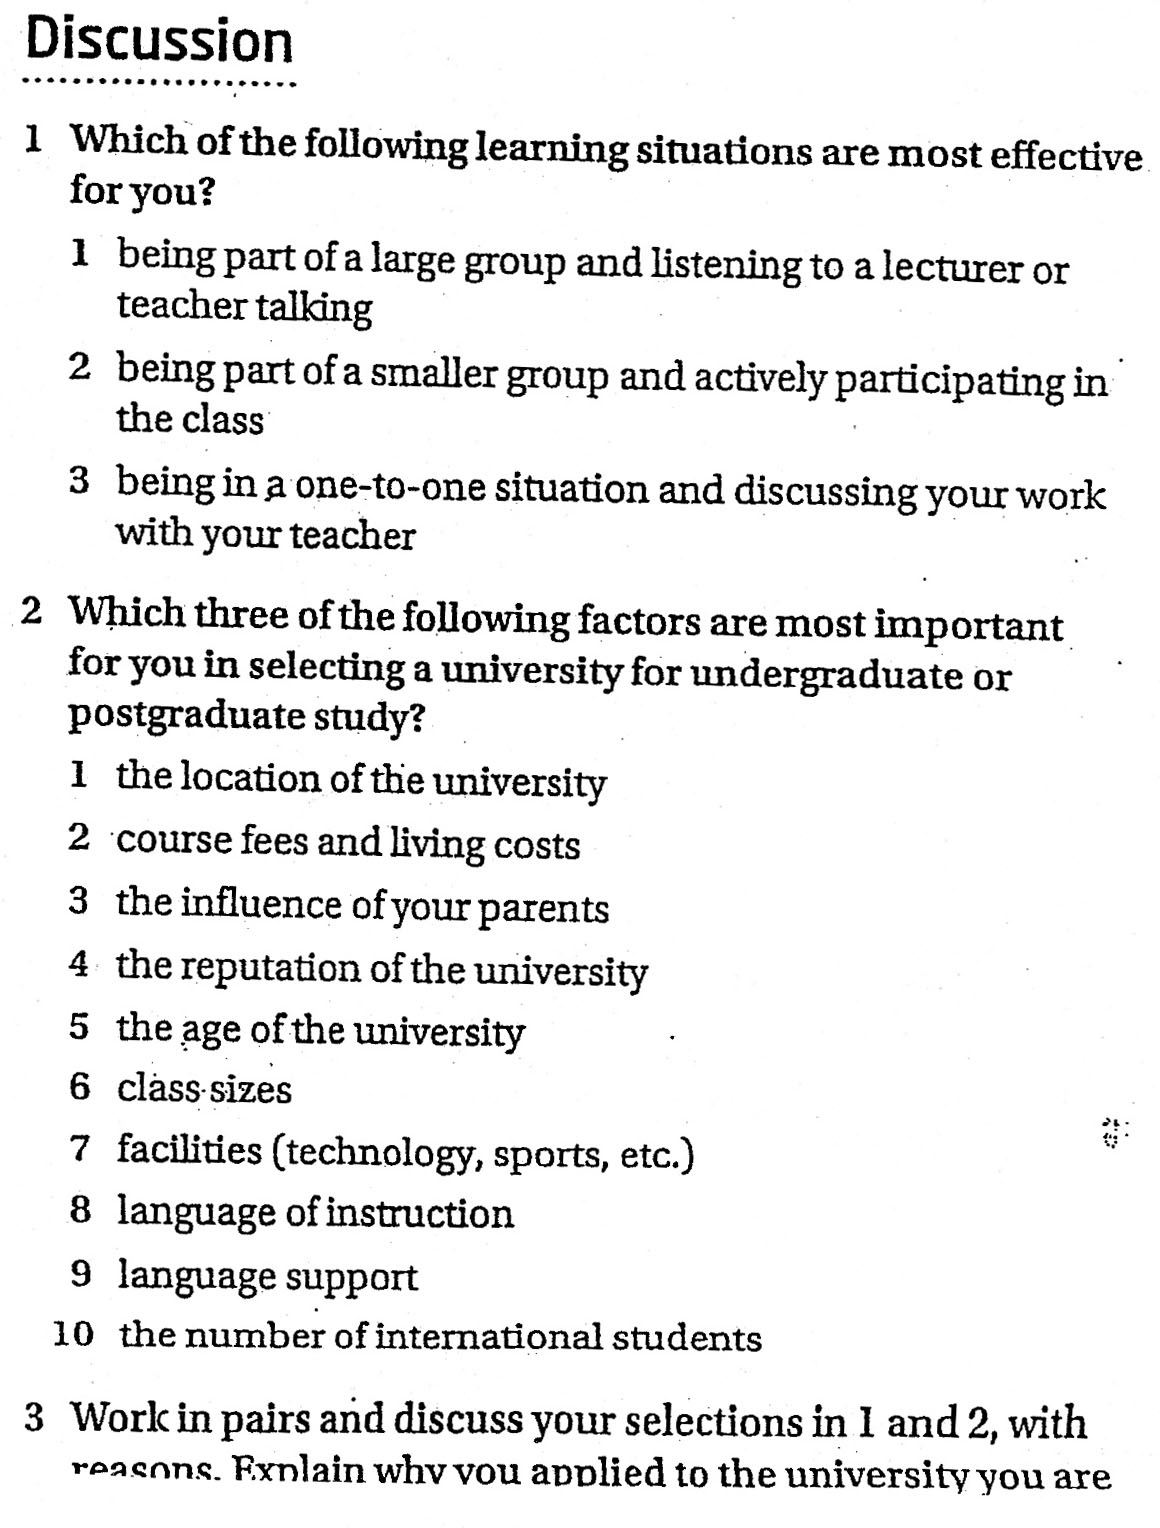
\includegraphics[scale=.85]{handouts/Eng101.jpg}

%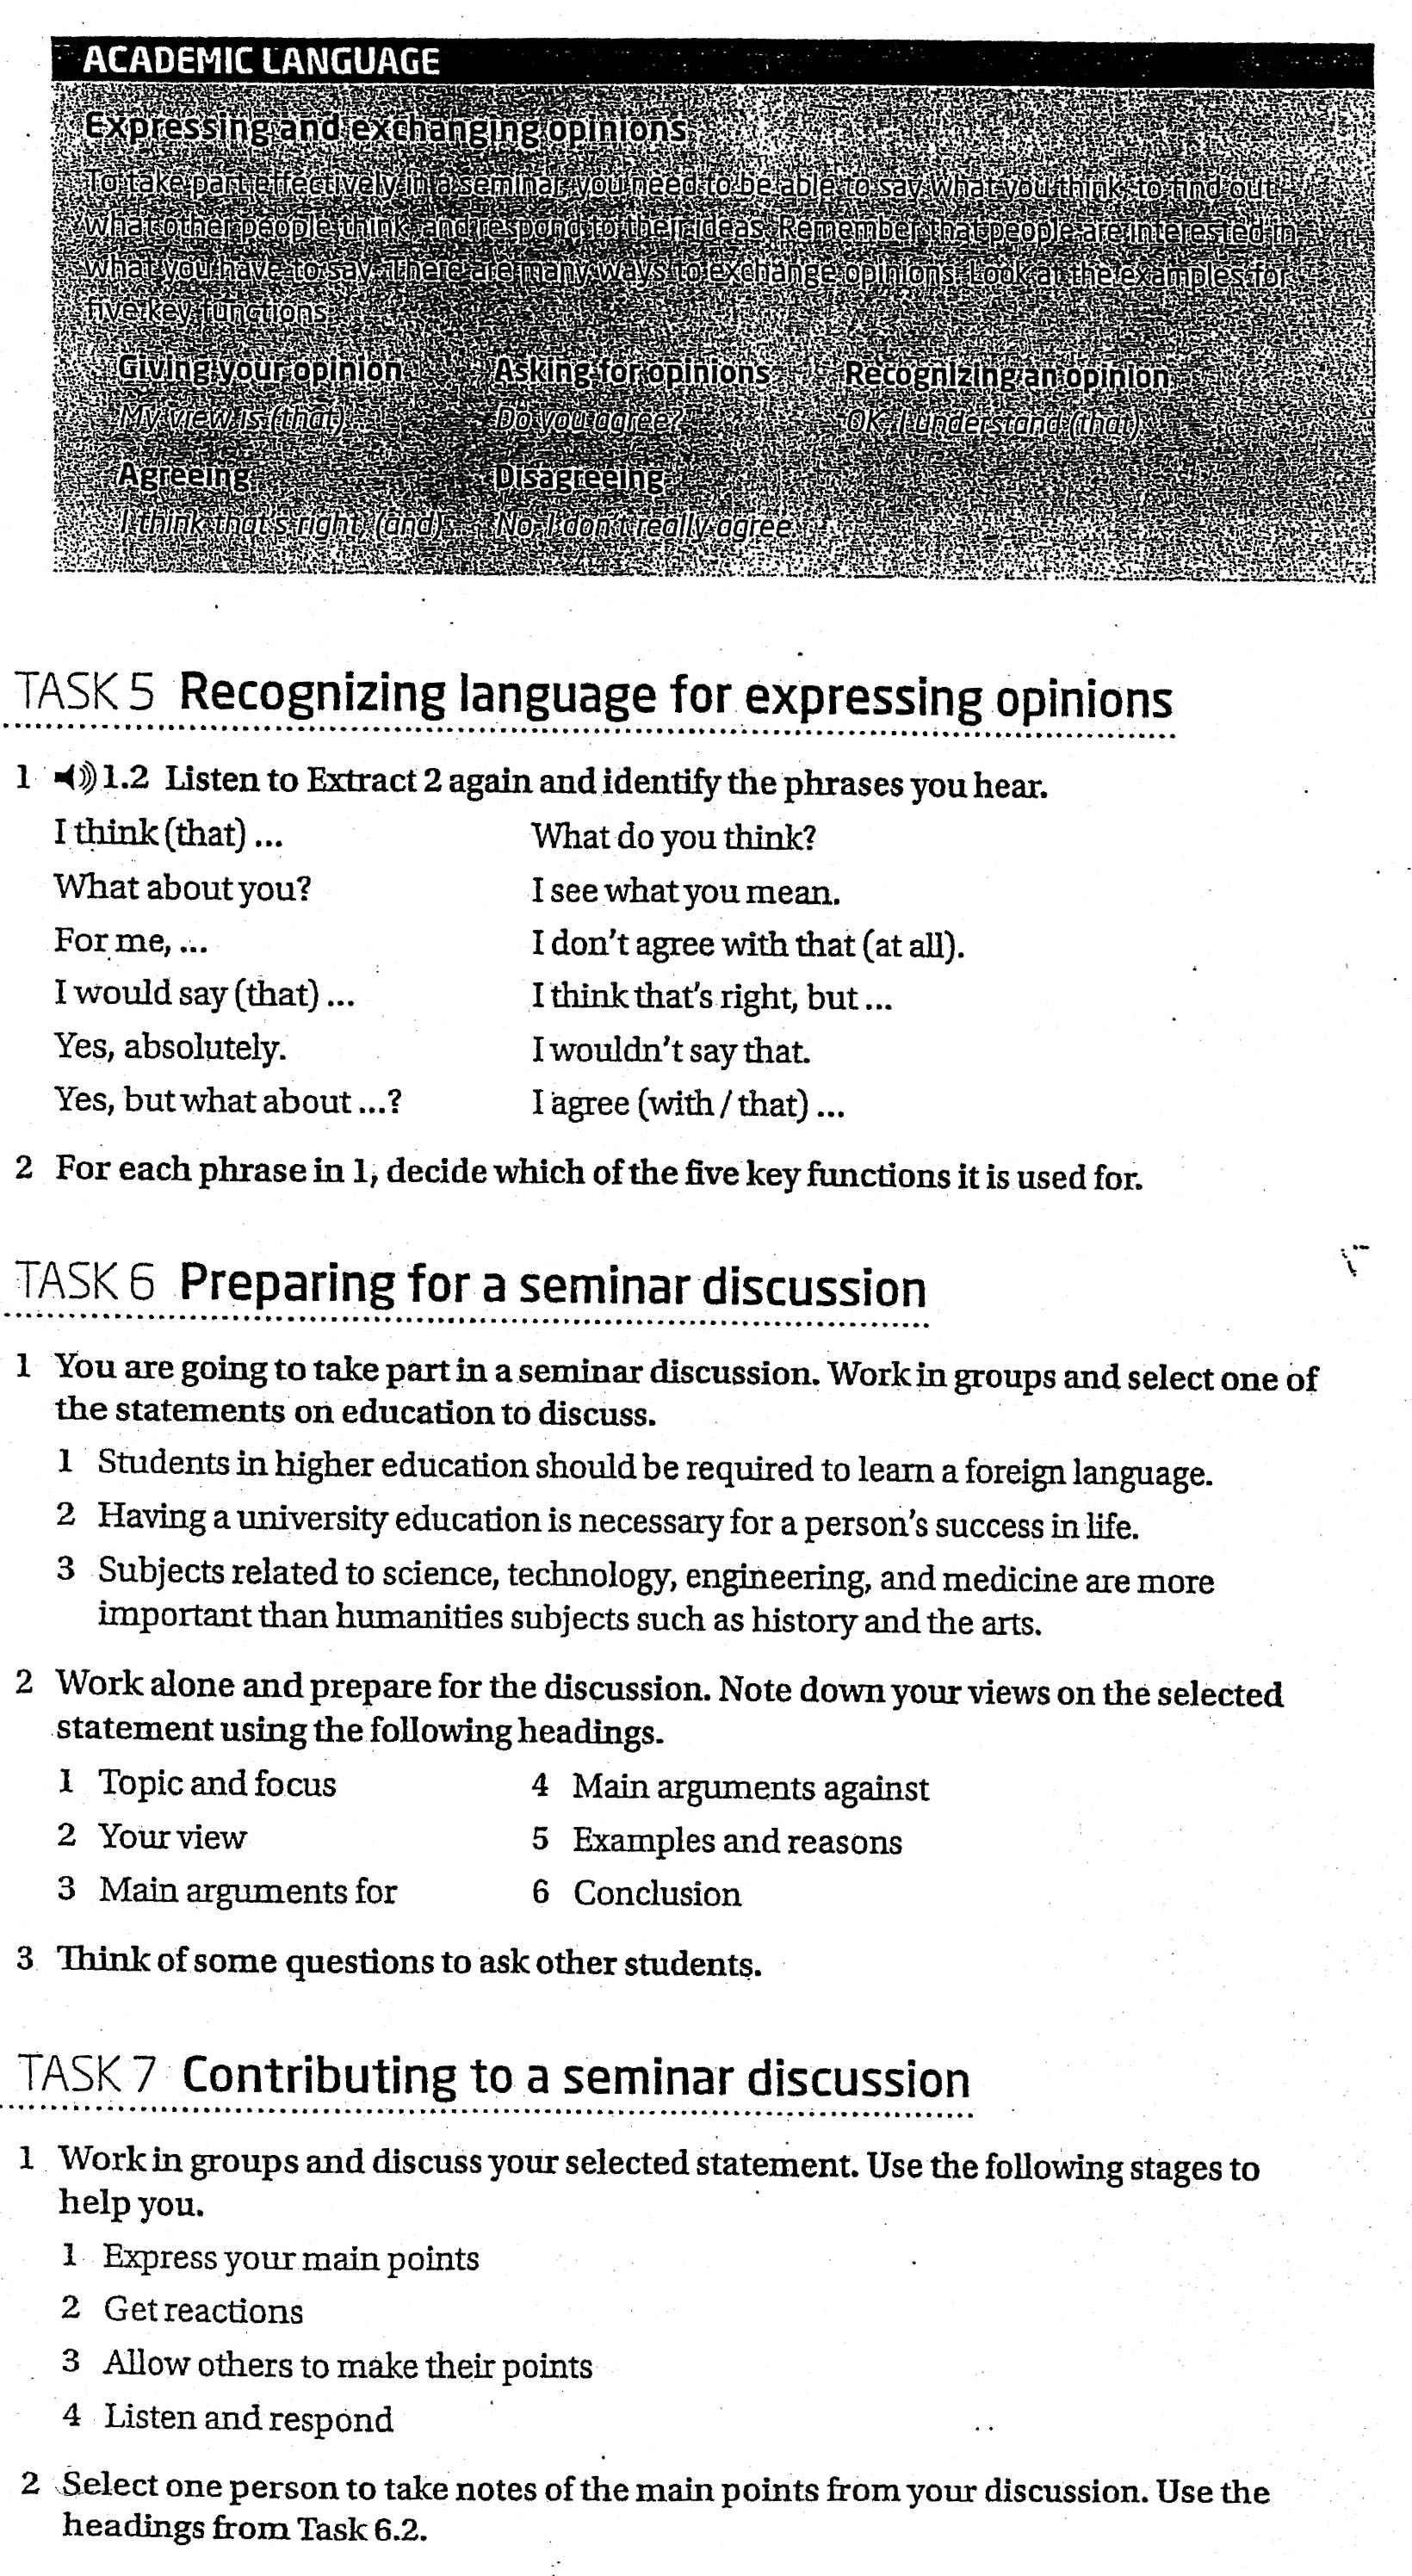
\includegraphics[scale=.85]{handouts/Eng102.jpg}
\section{Conditionals}
%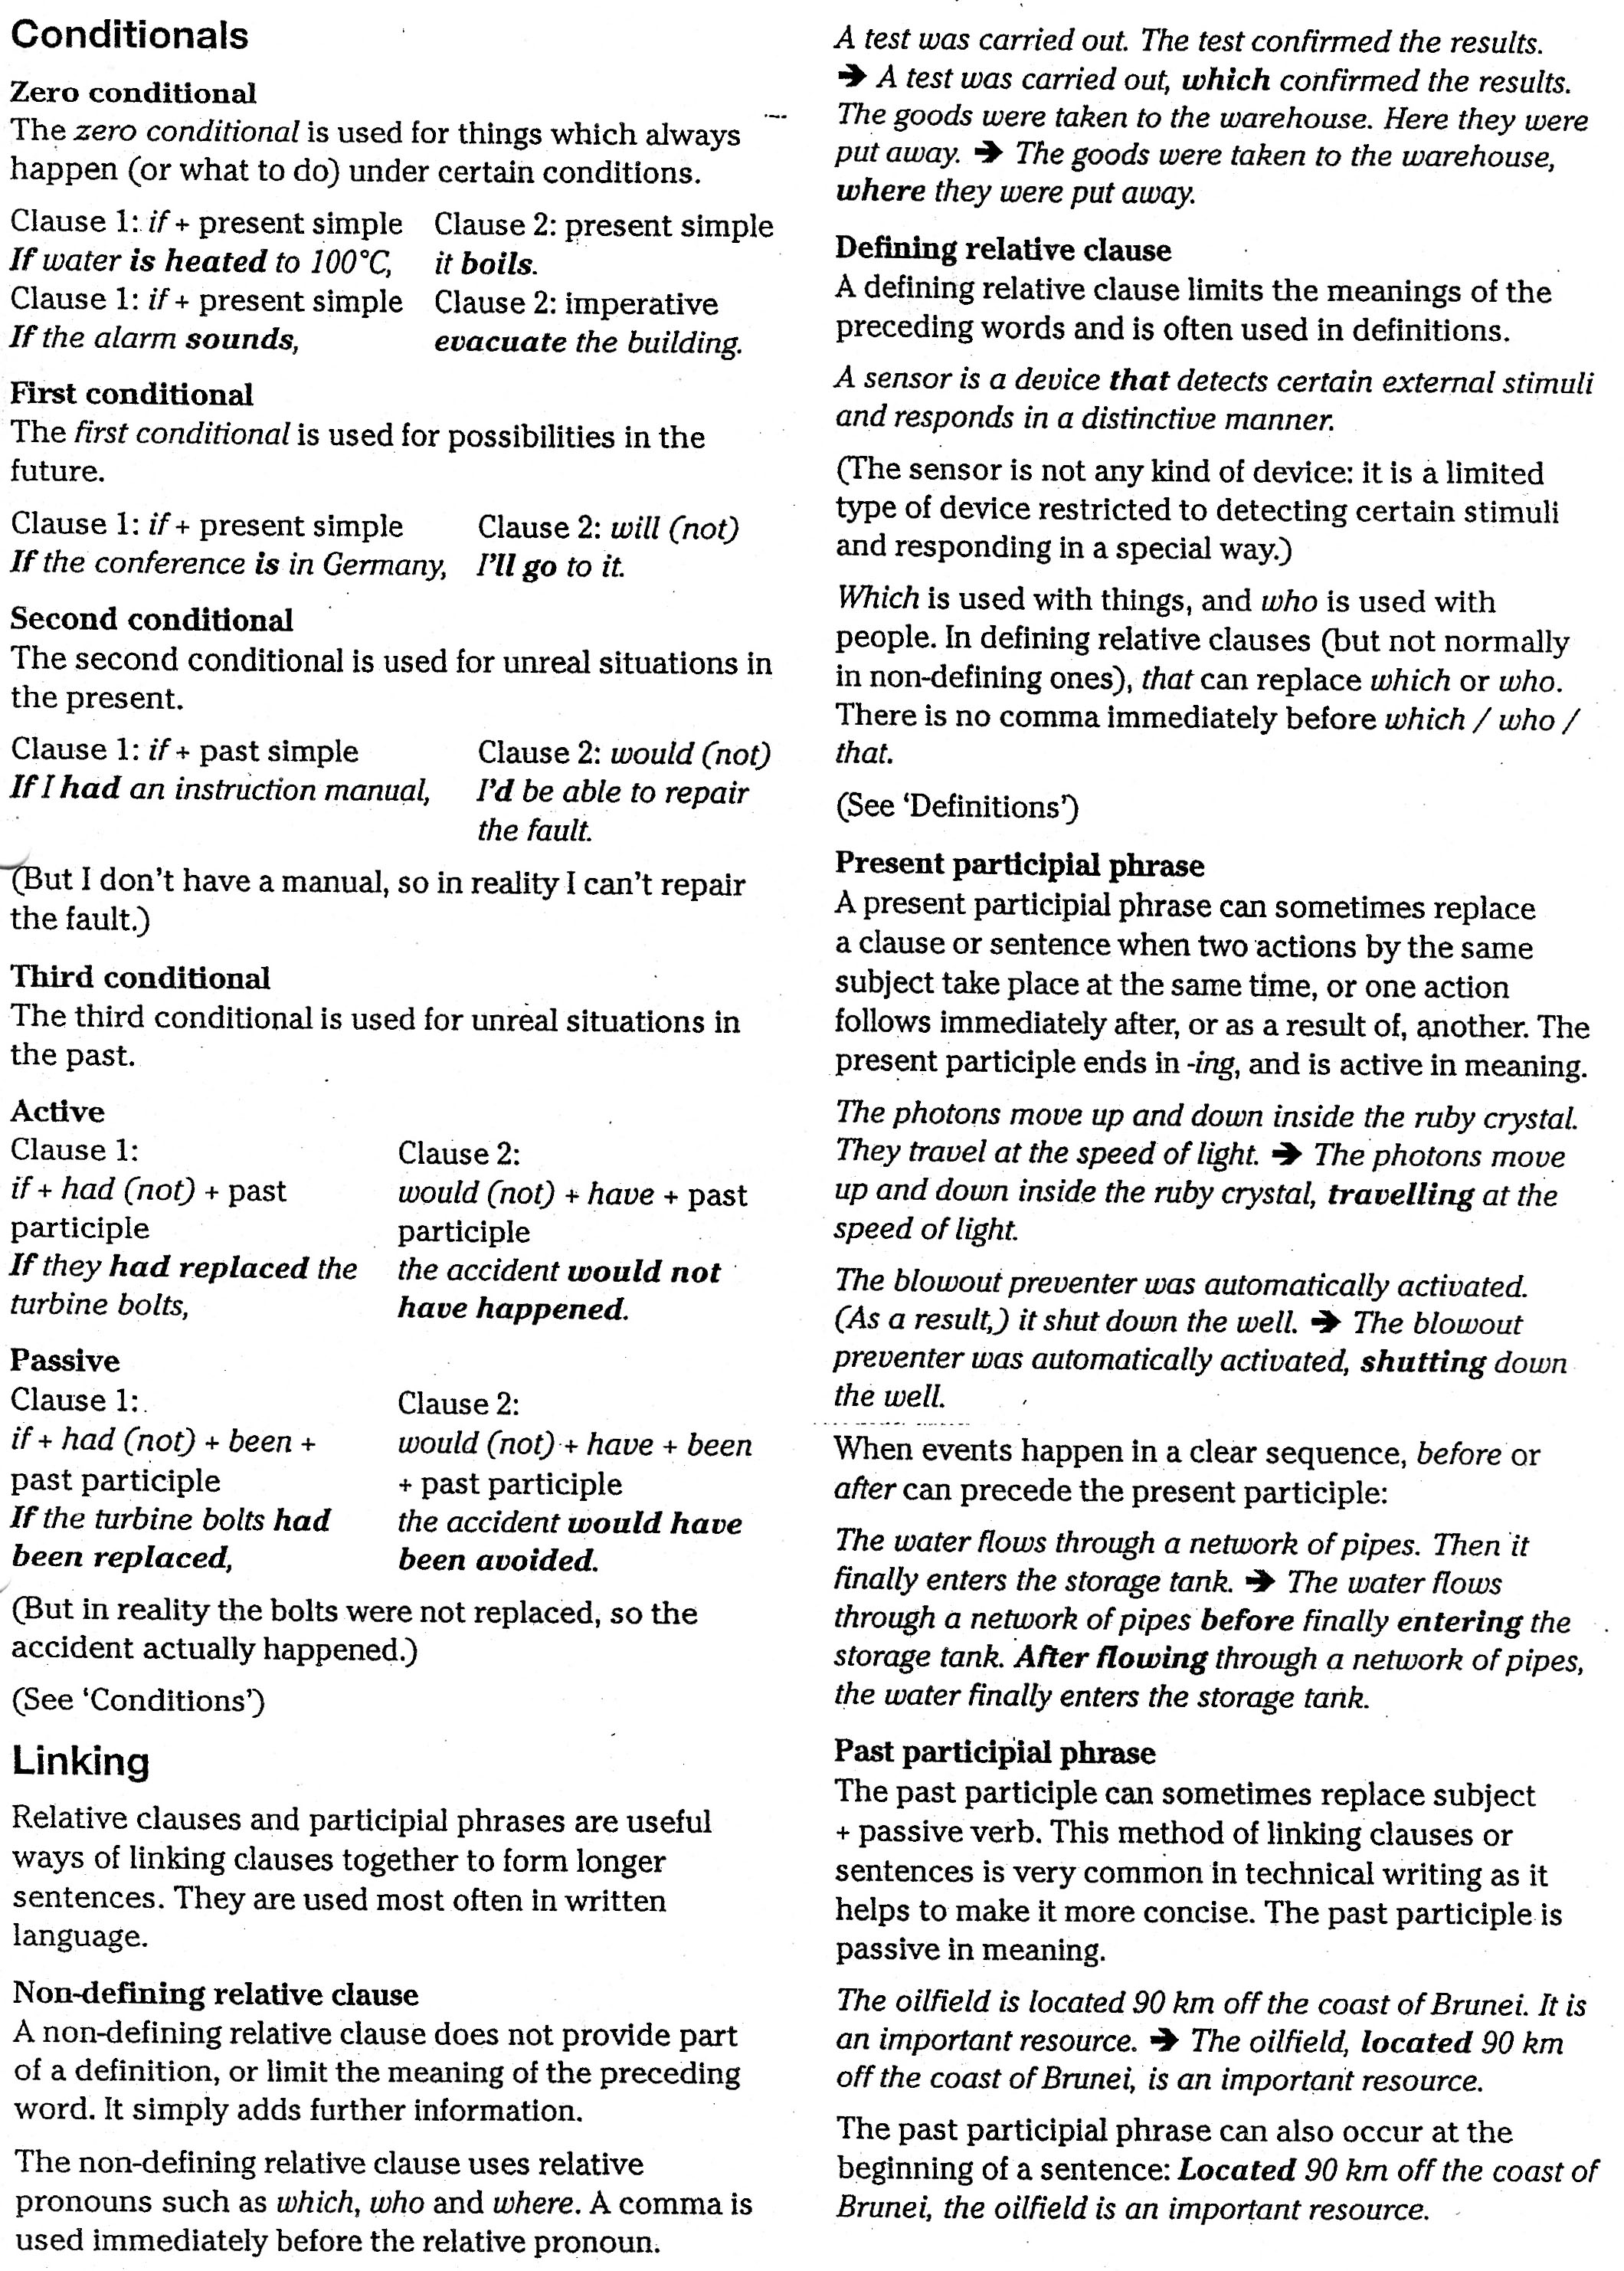
\includegraphics[scale=.85]{handouts/Eng103.jpg}

%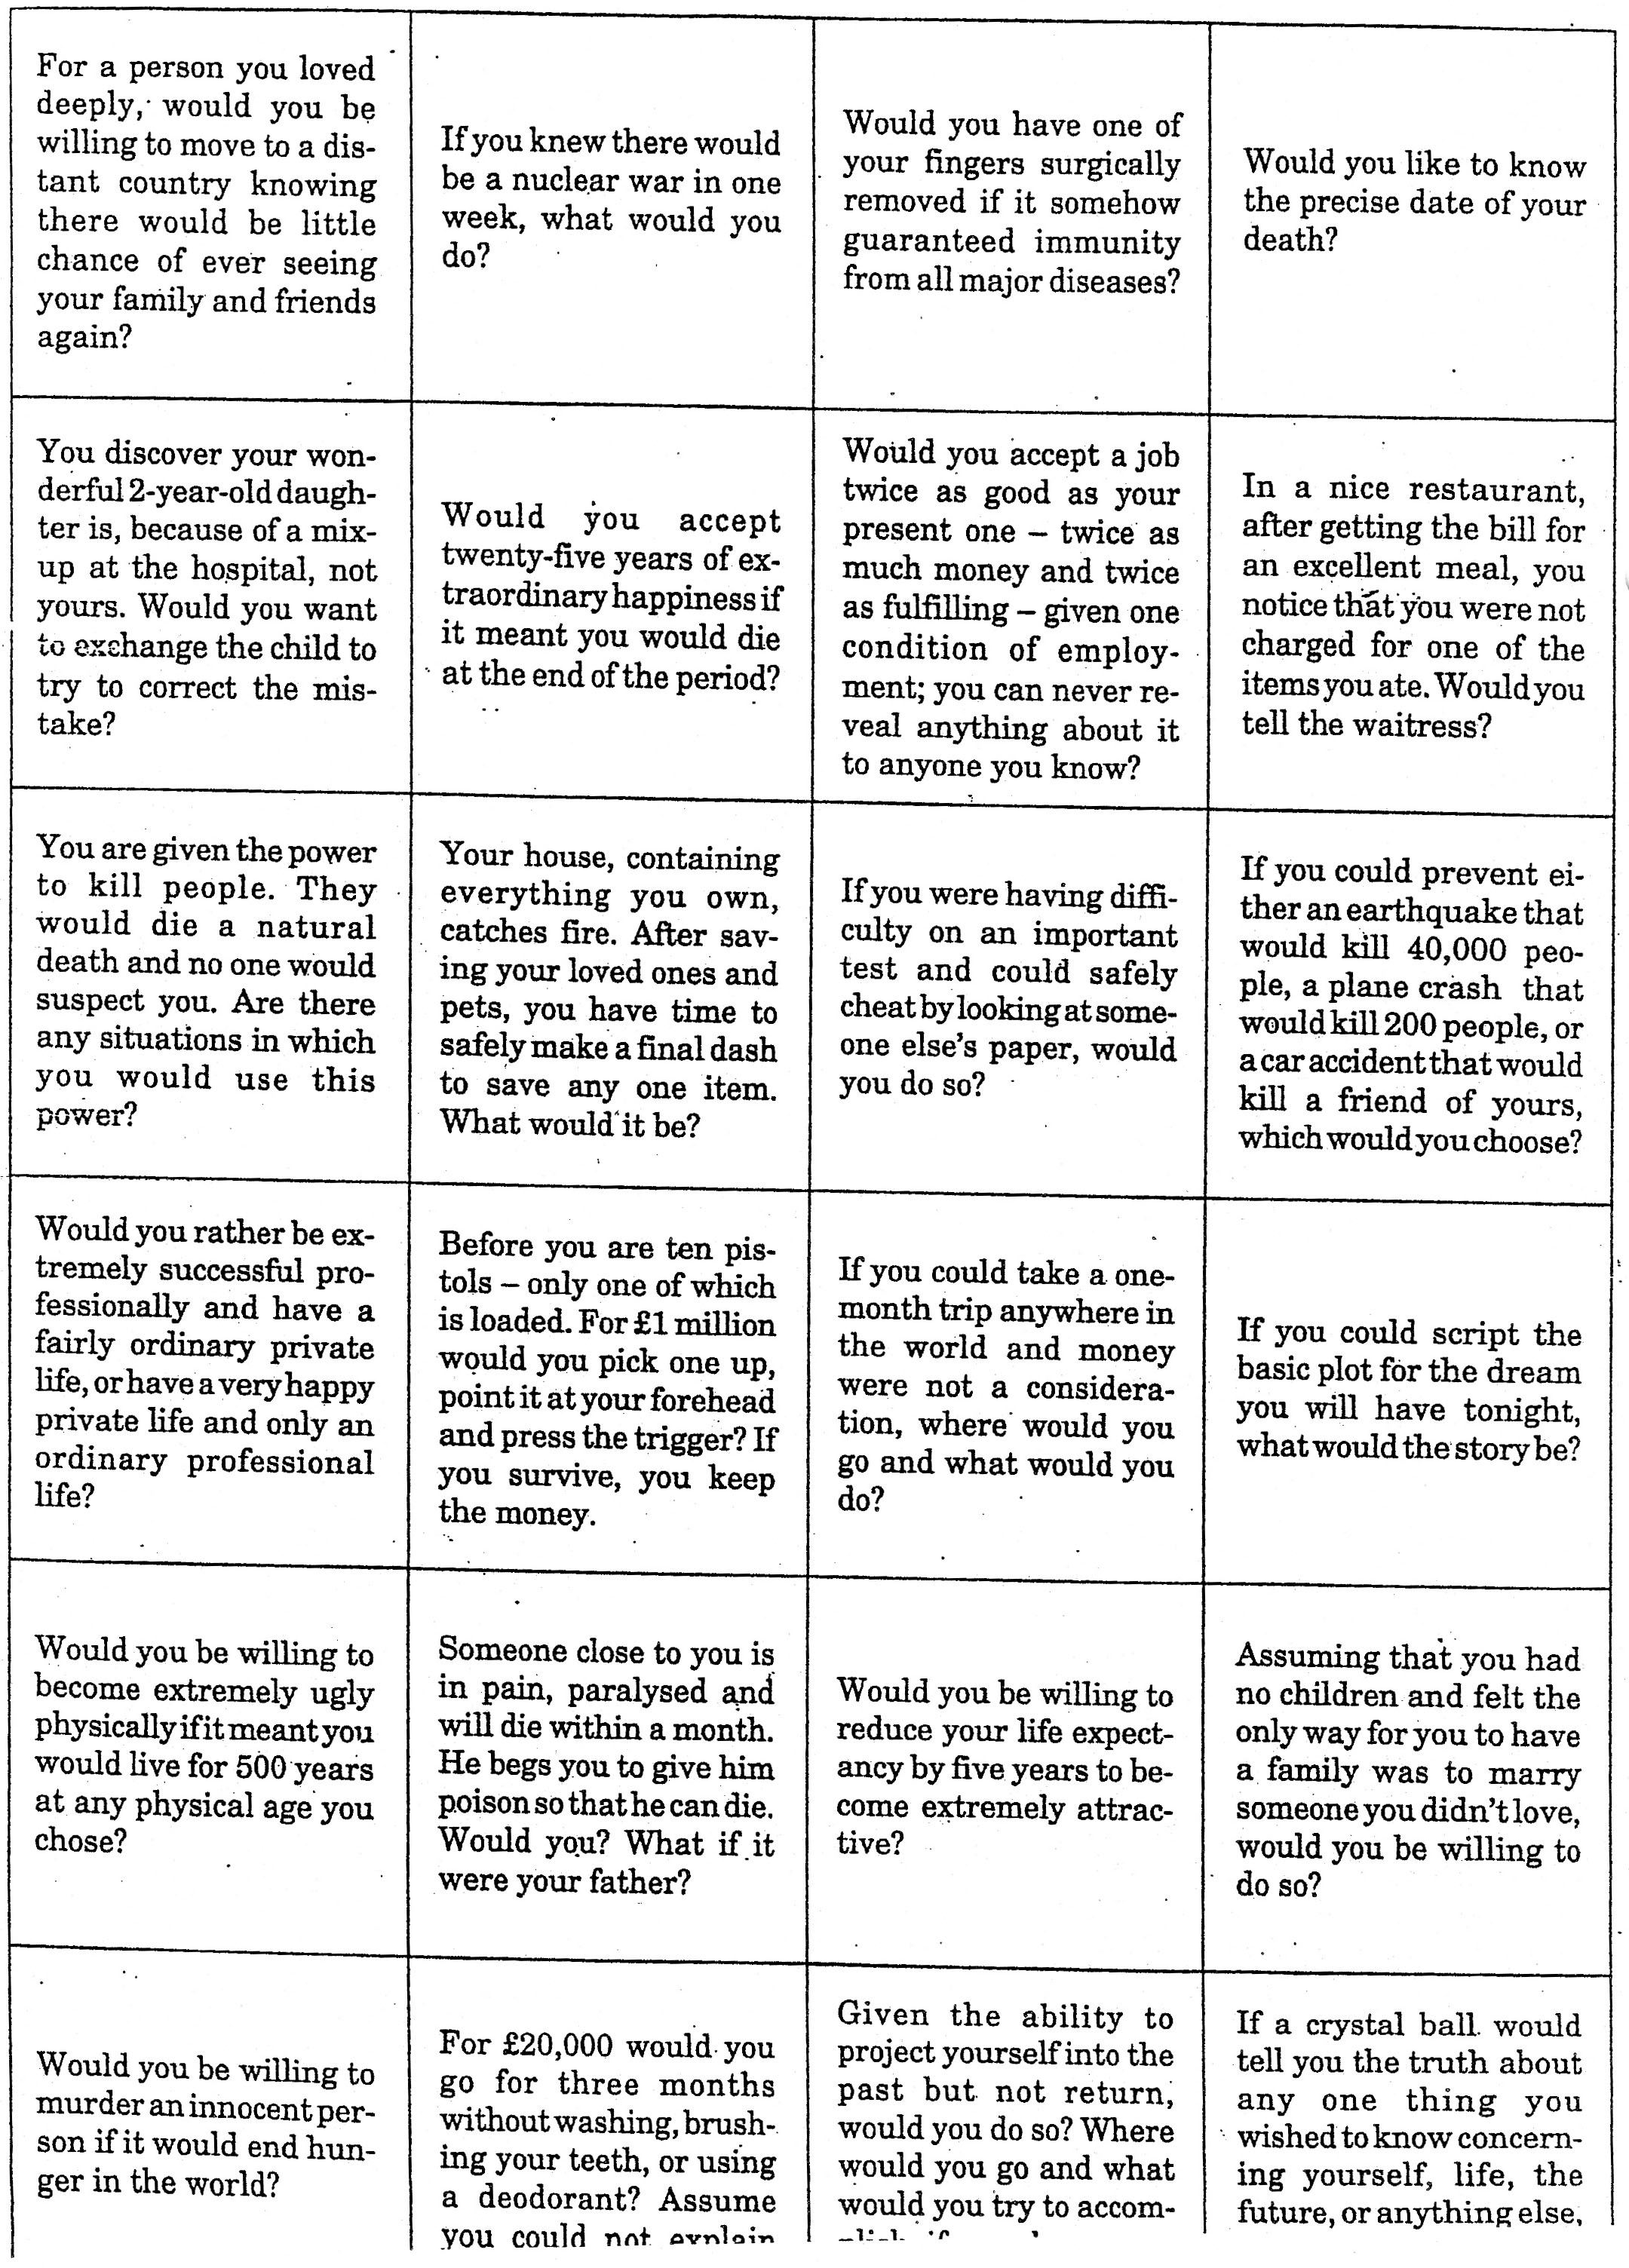
\includegraphics[scale=.85]{handouts/Eng104.jpg}
\section{Conditional sentences: verb tenses}
%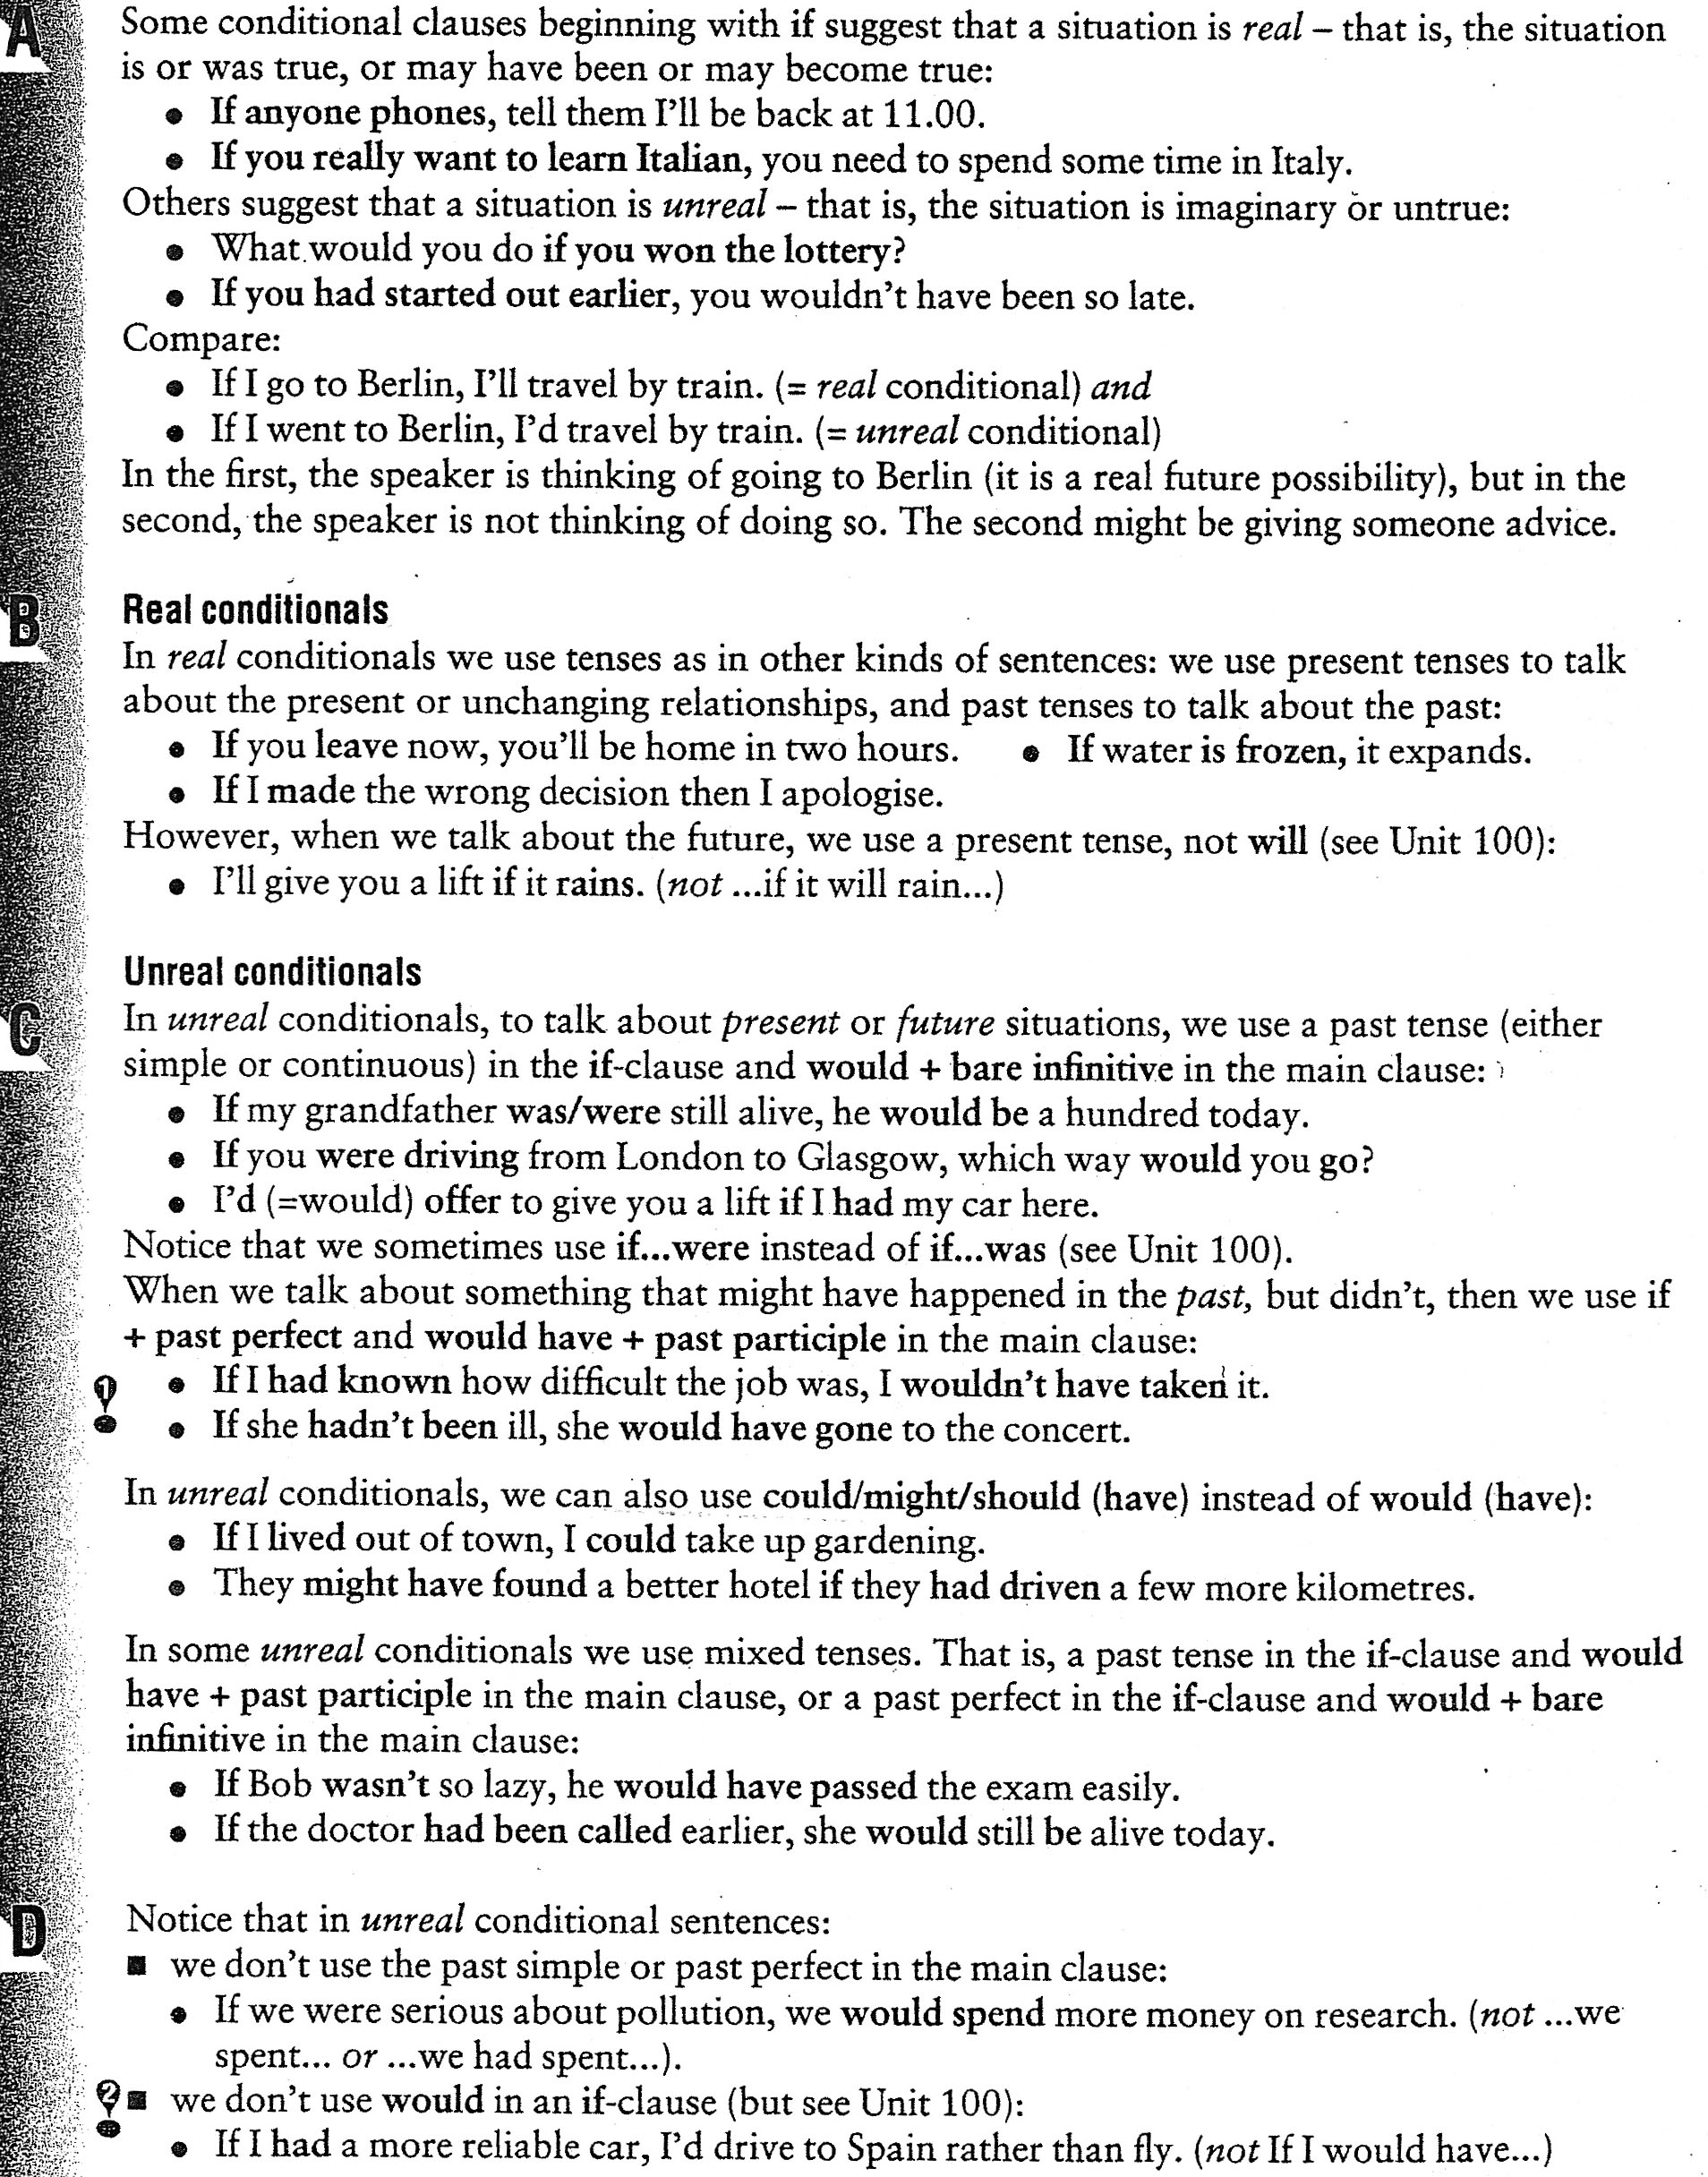
\includegraphics[scale=.85]{handouts/Eng105.jpg}

%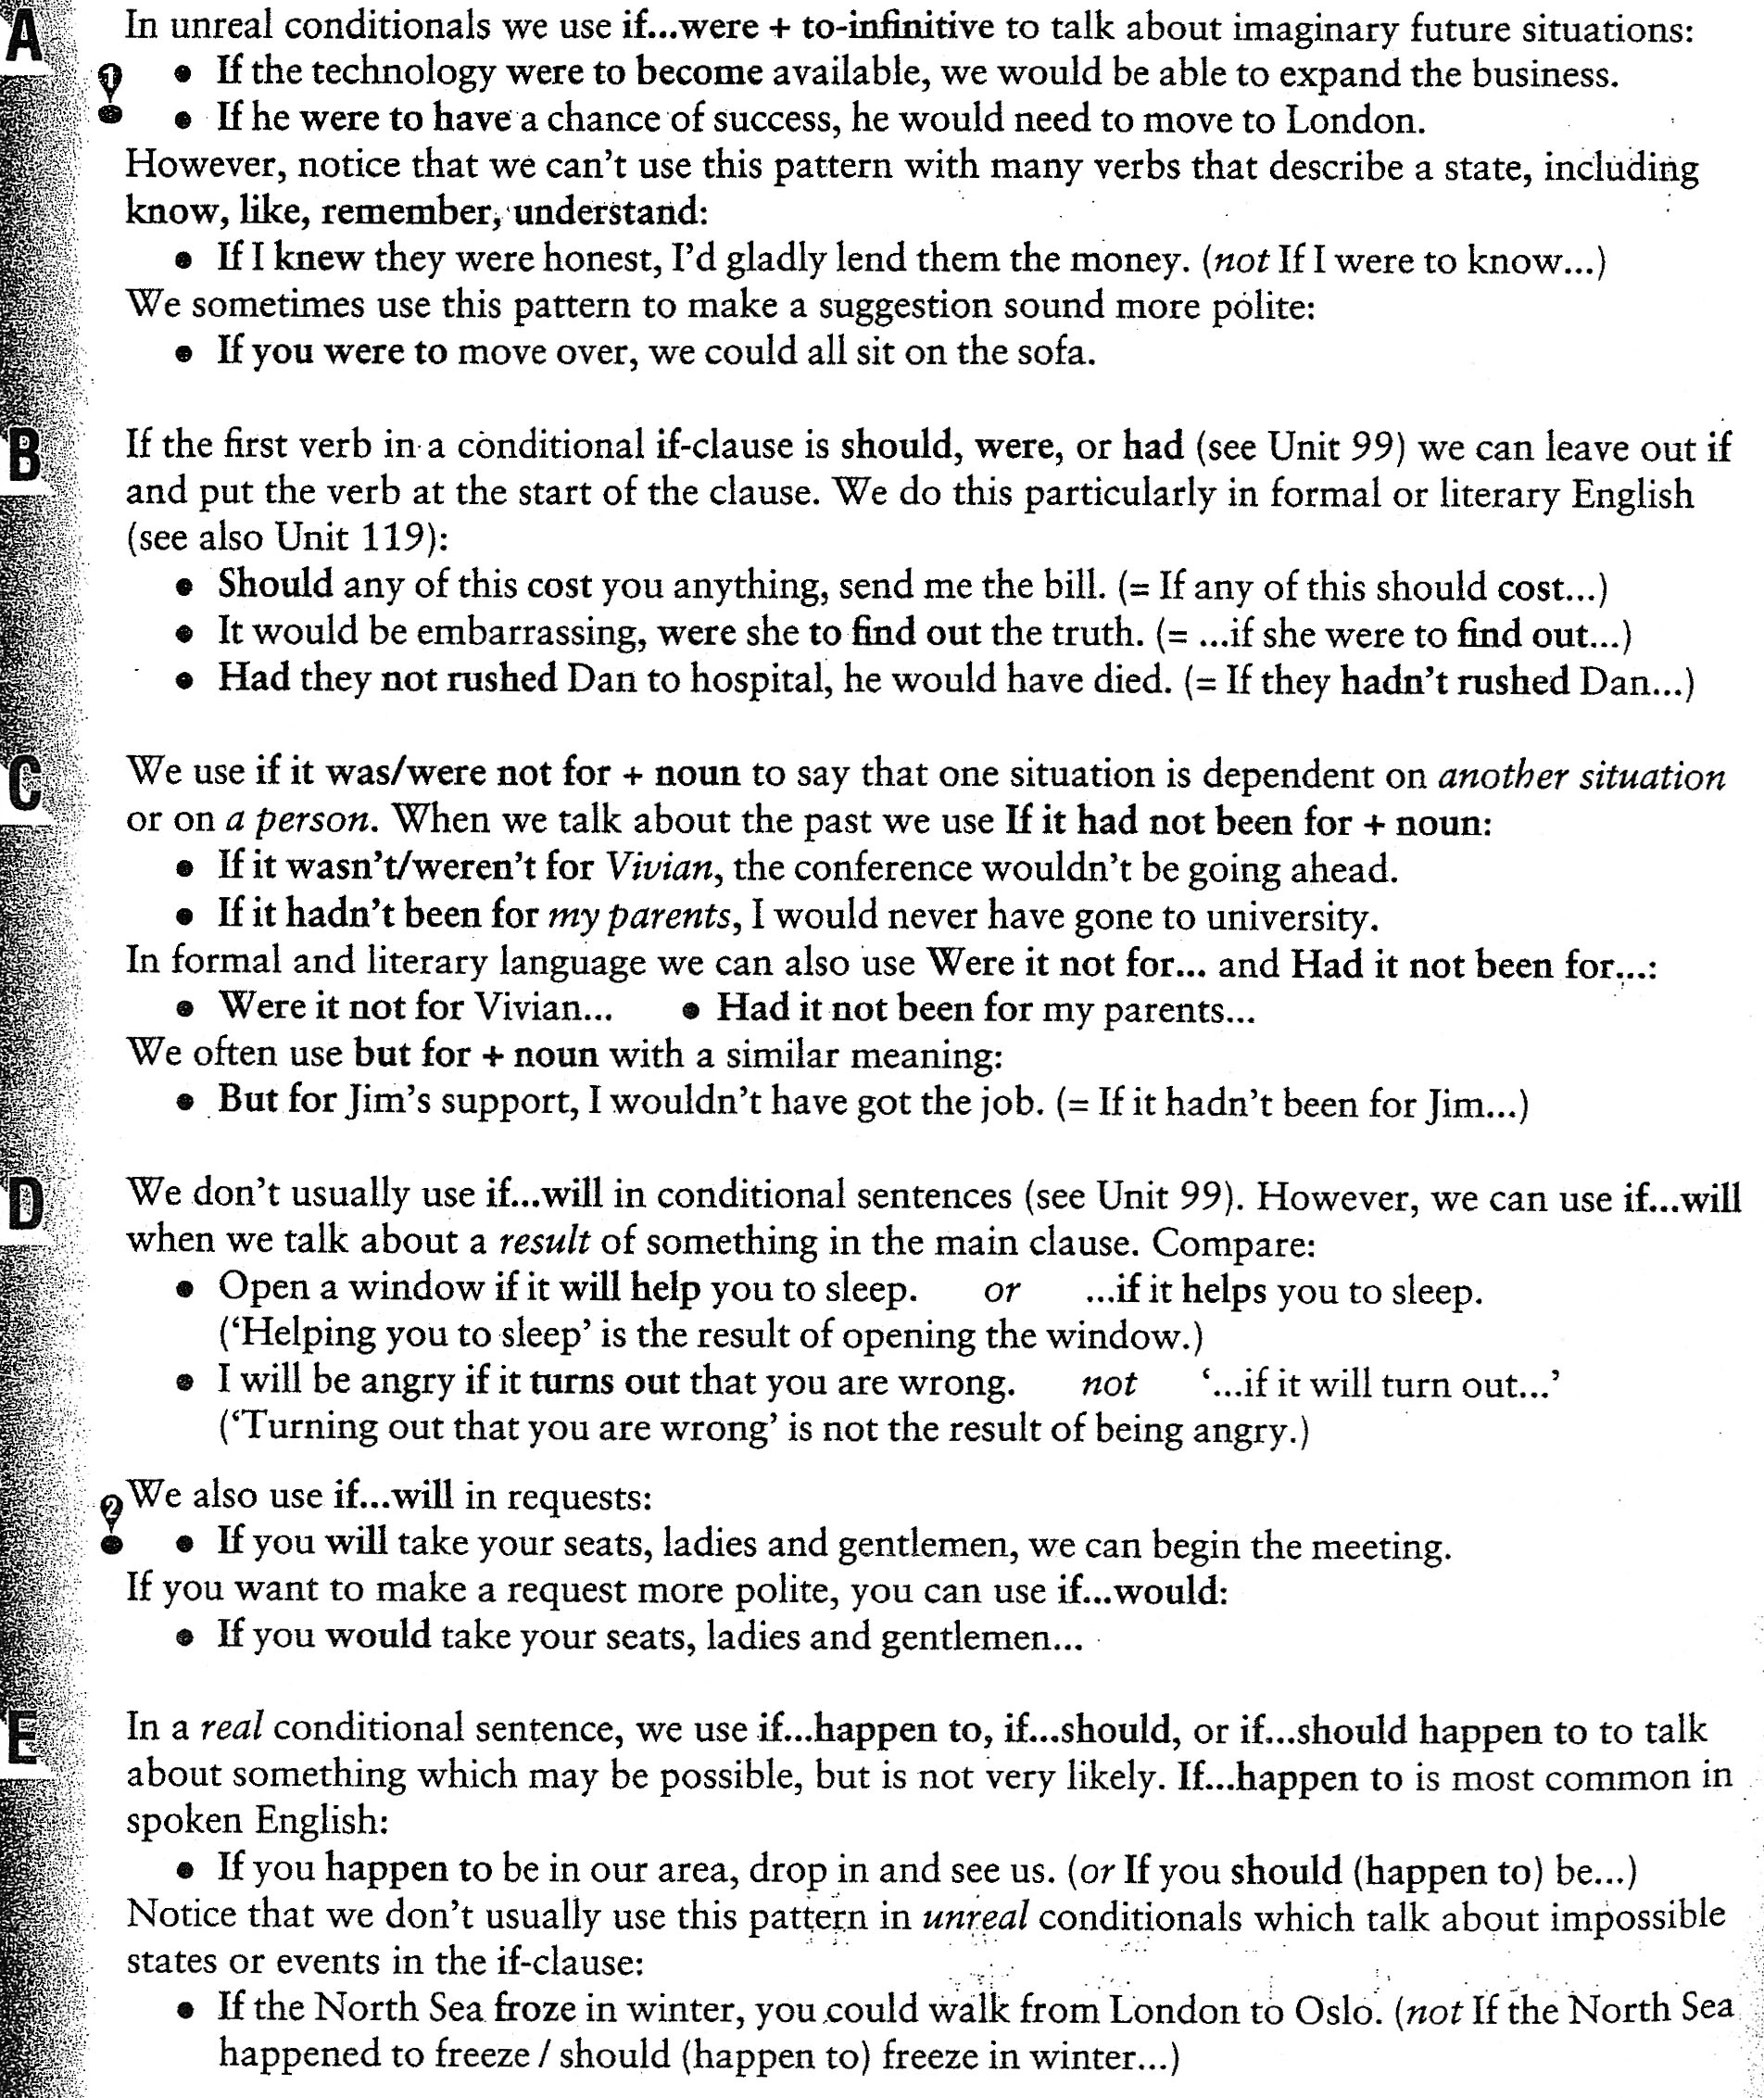
\includegraphics[scale=.85]{handouts/Eng106.jpg}
\section{Exercises}
%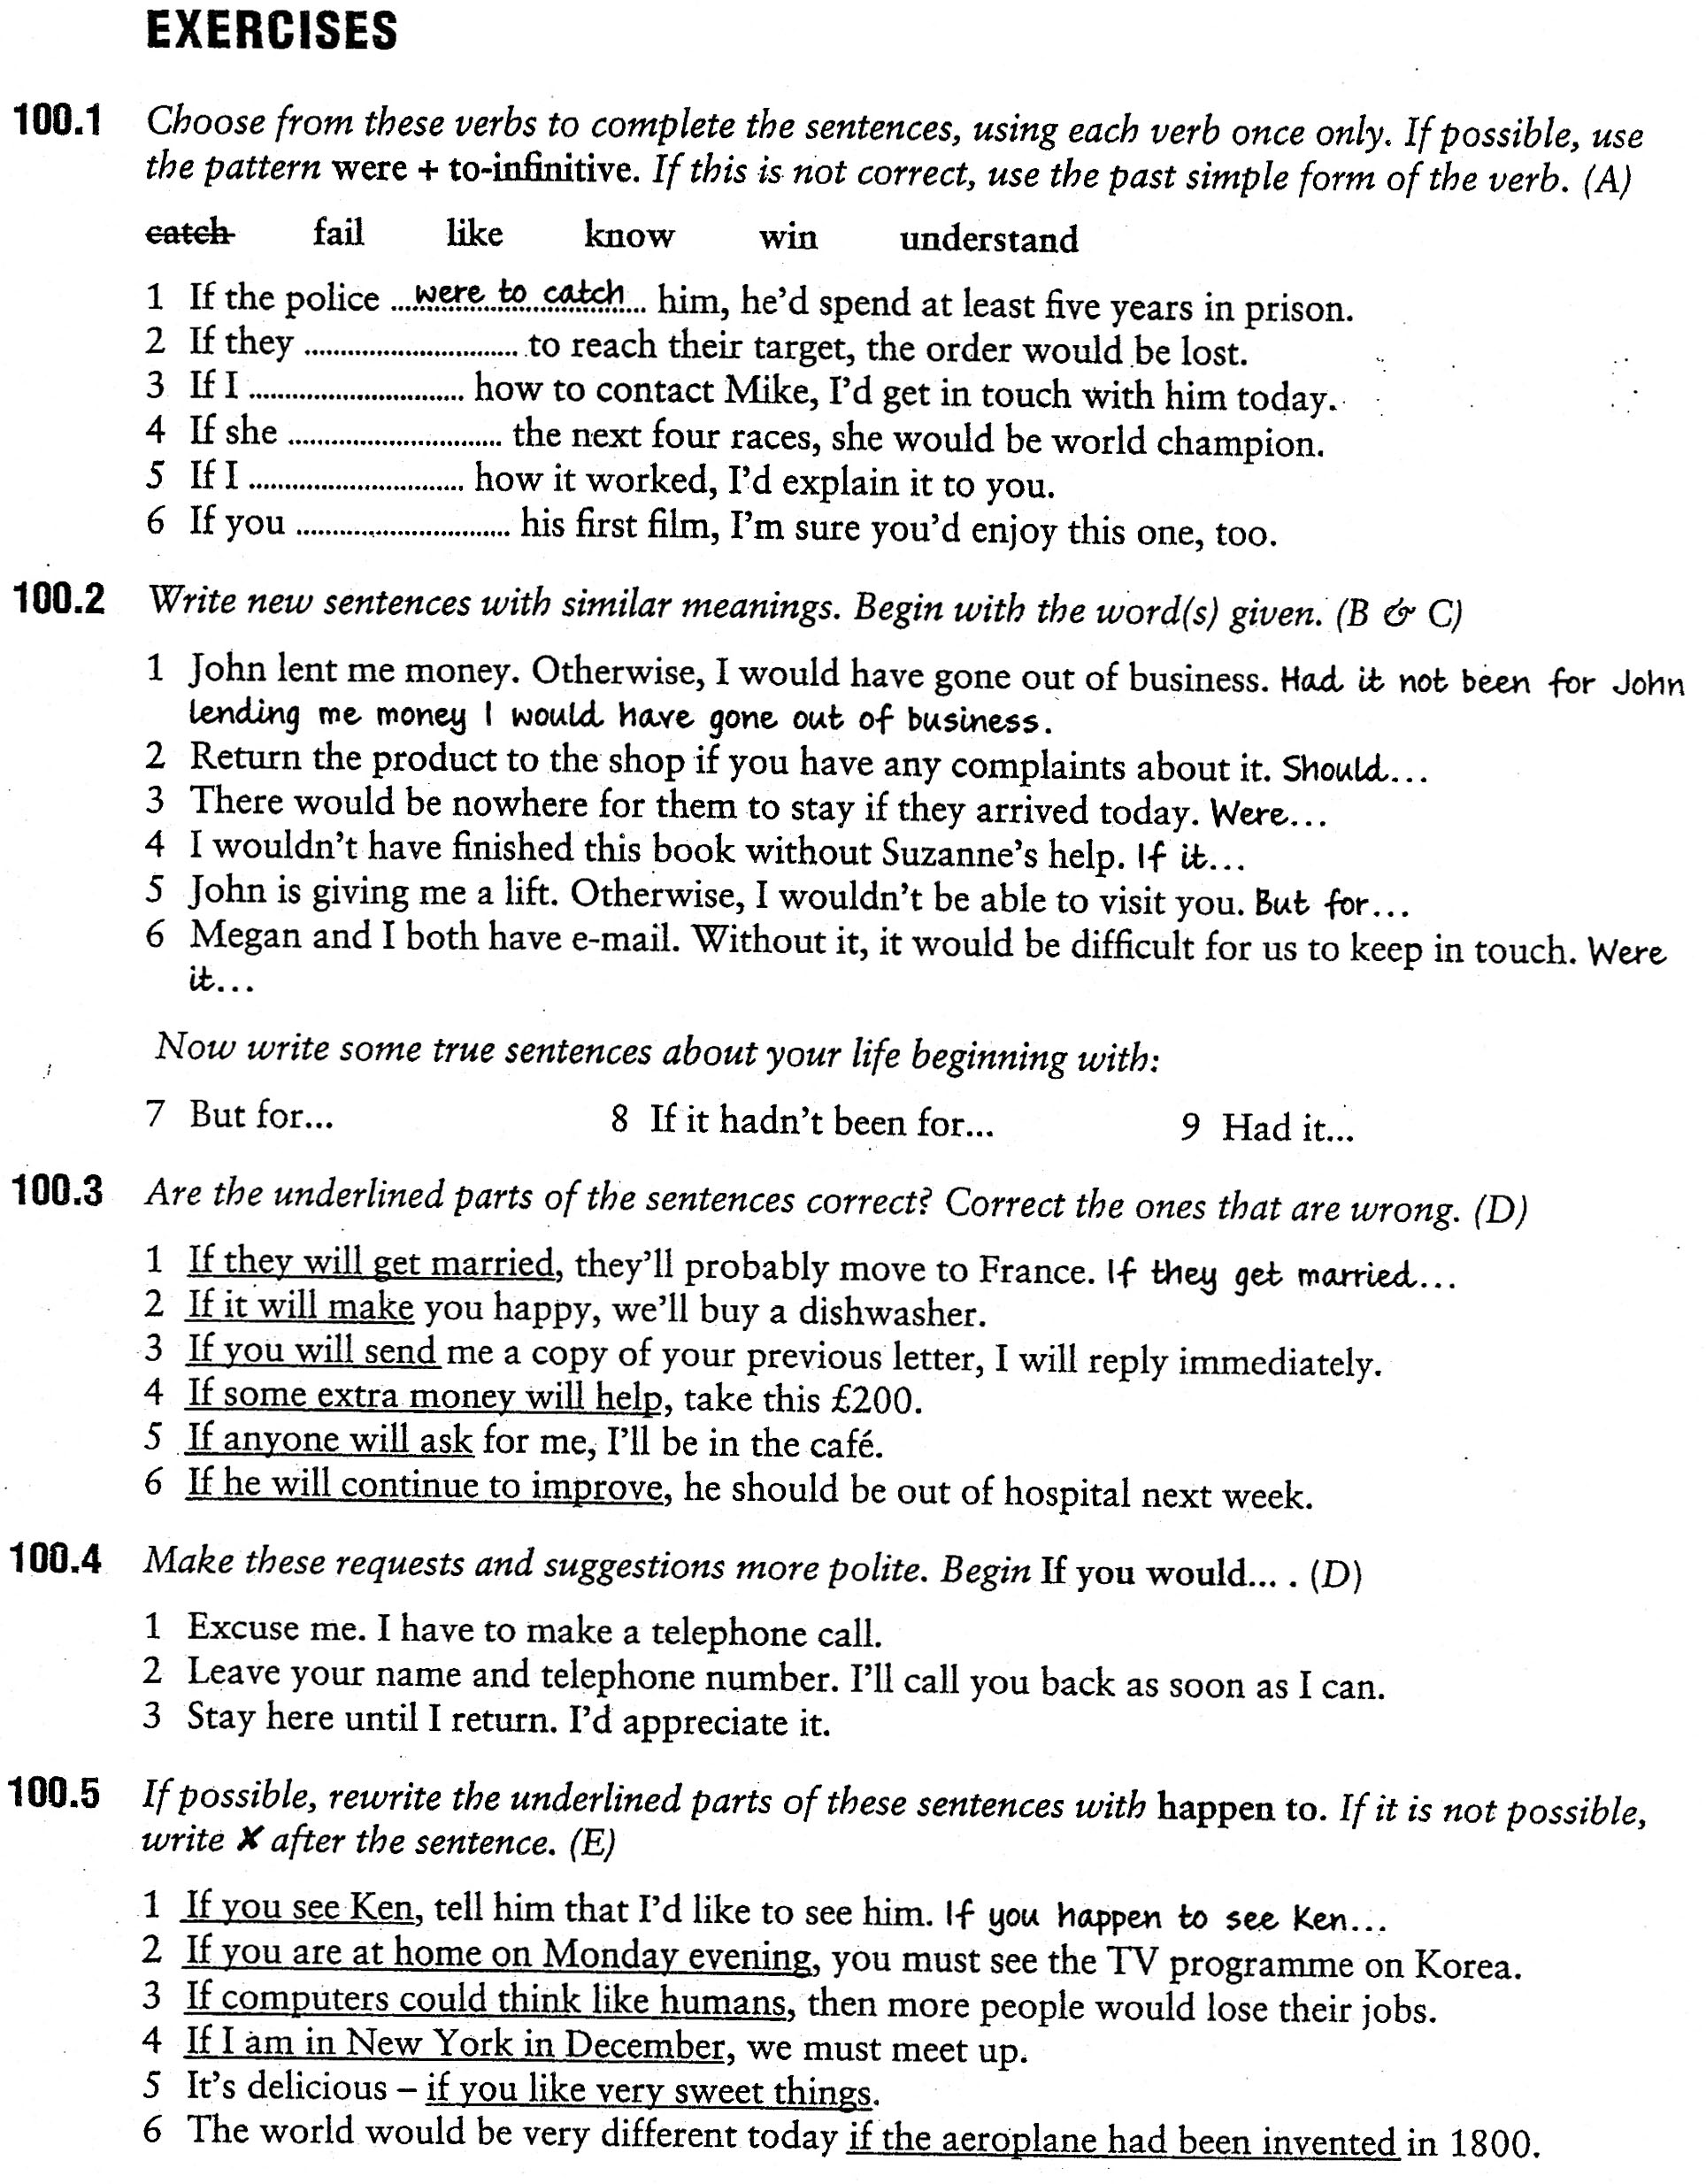
\includegraphics[scale=.85]{handouts/Eng107.jpg}

%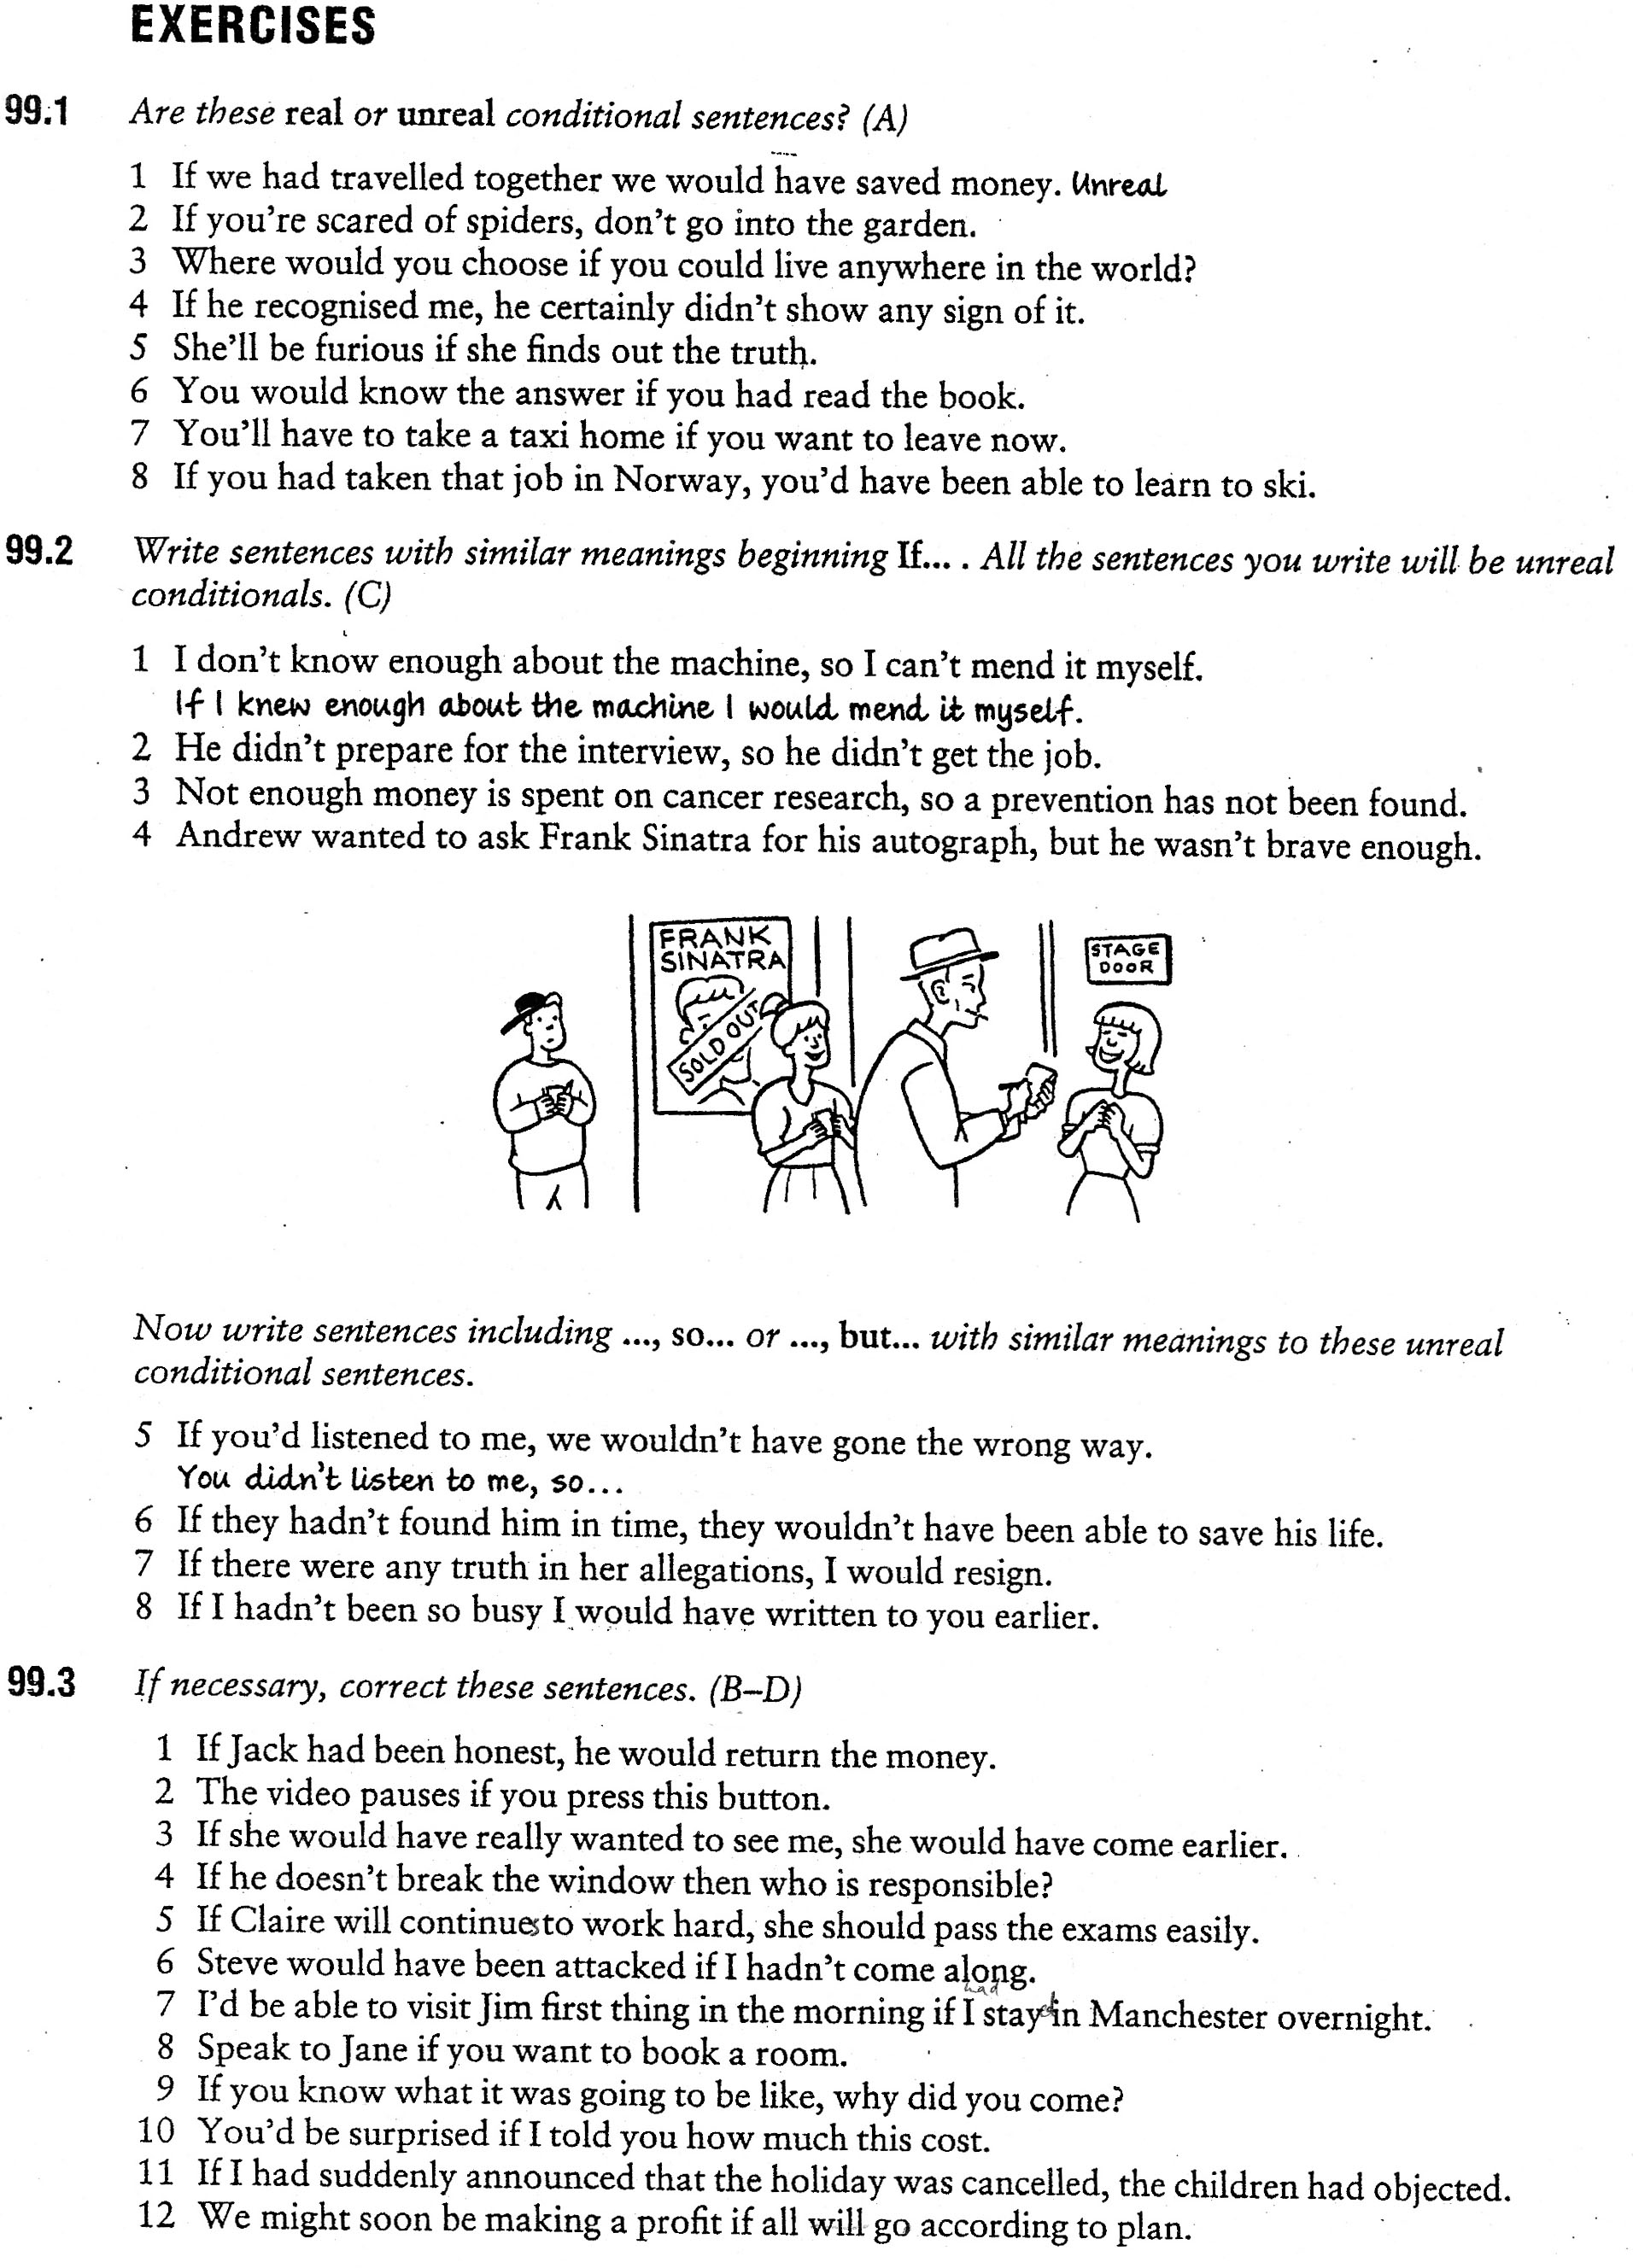
\includegraphics[scale=.85]{handouts/Eng108.jpg}

%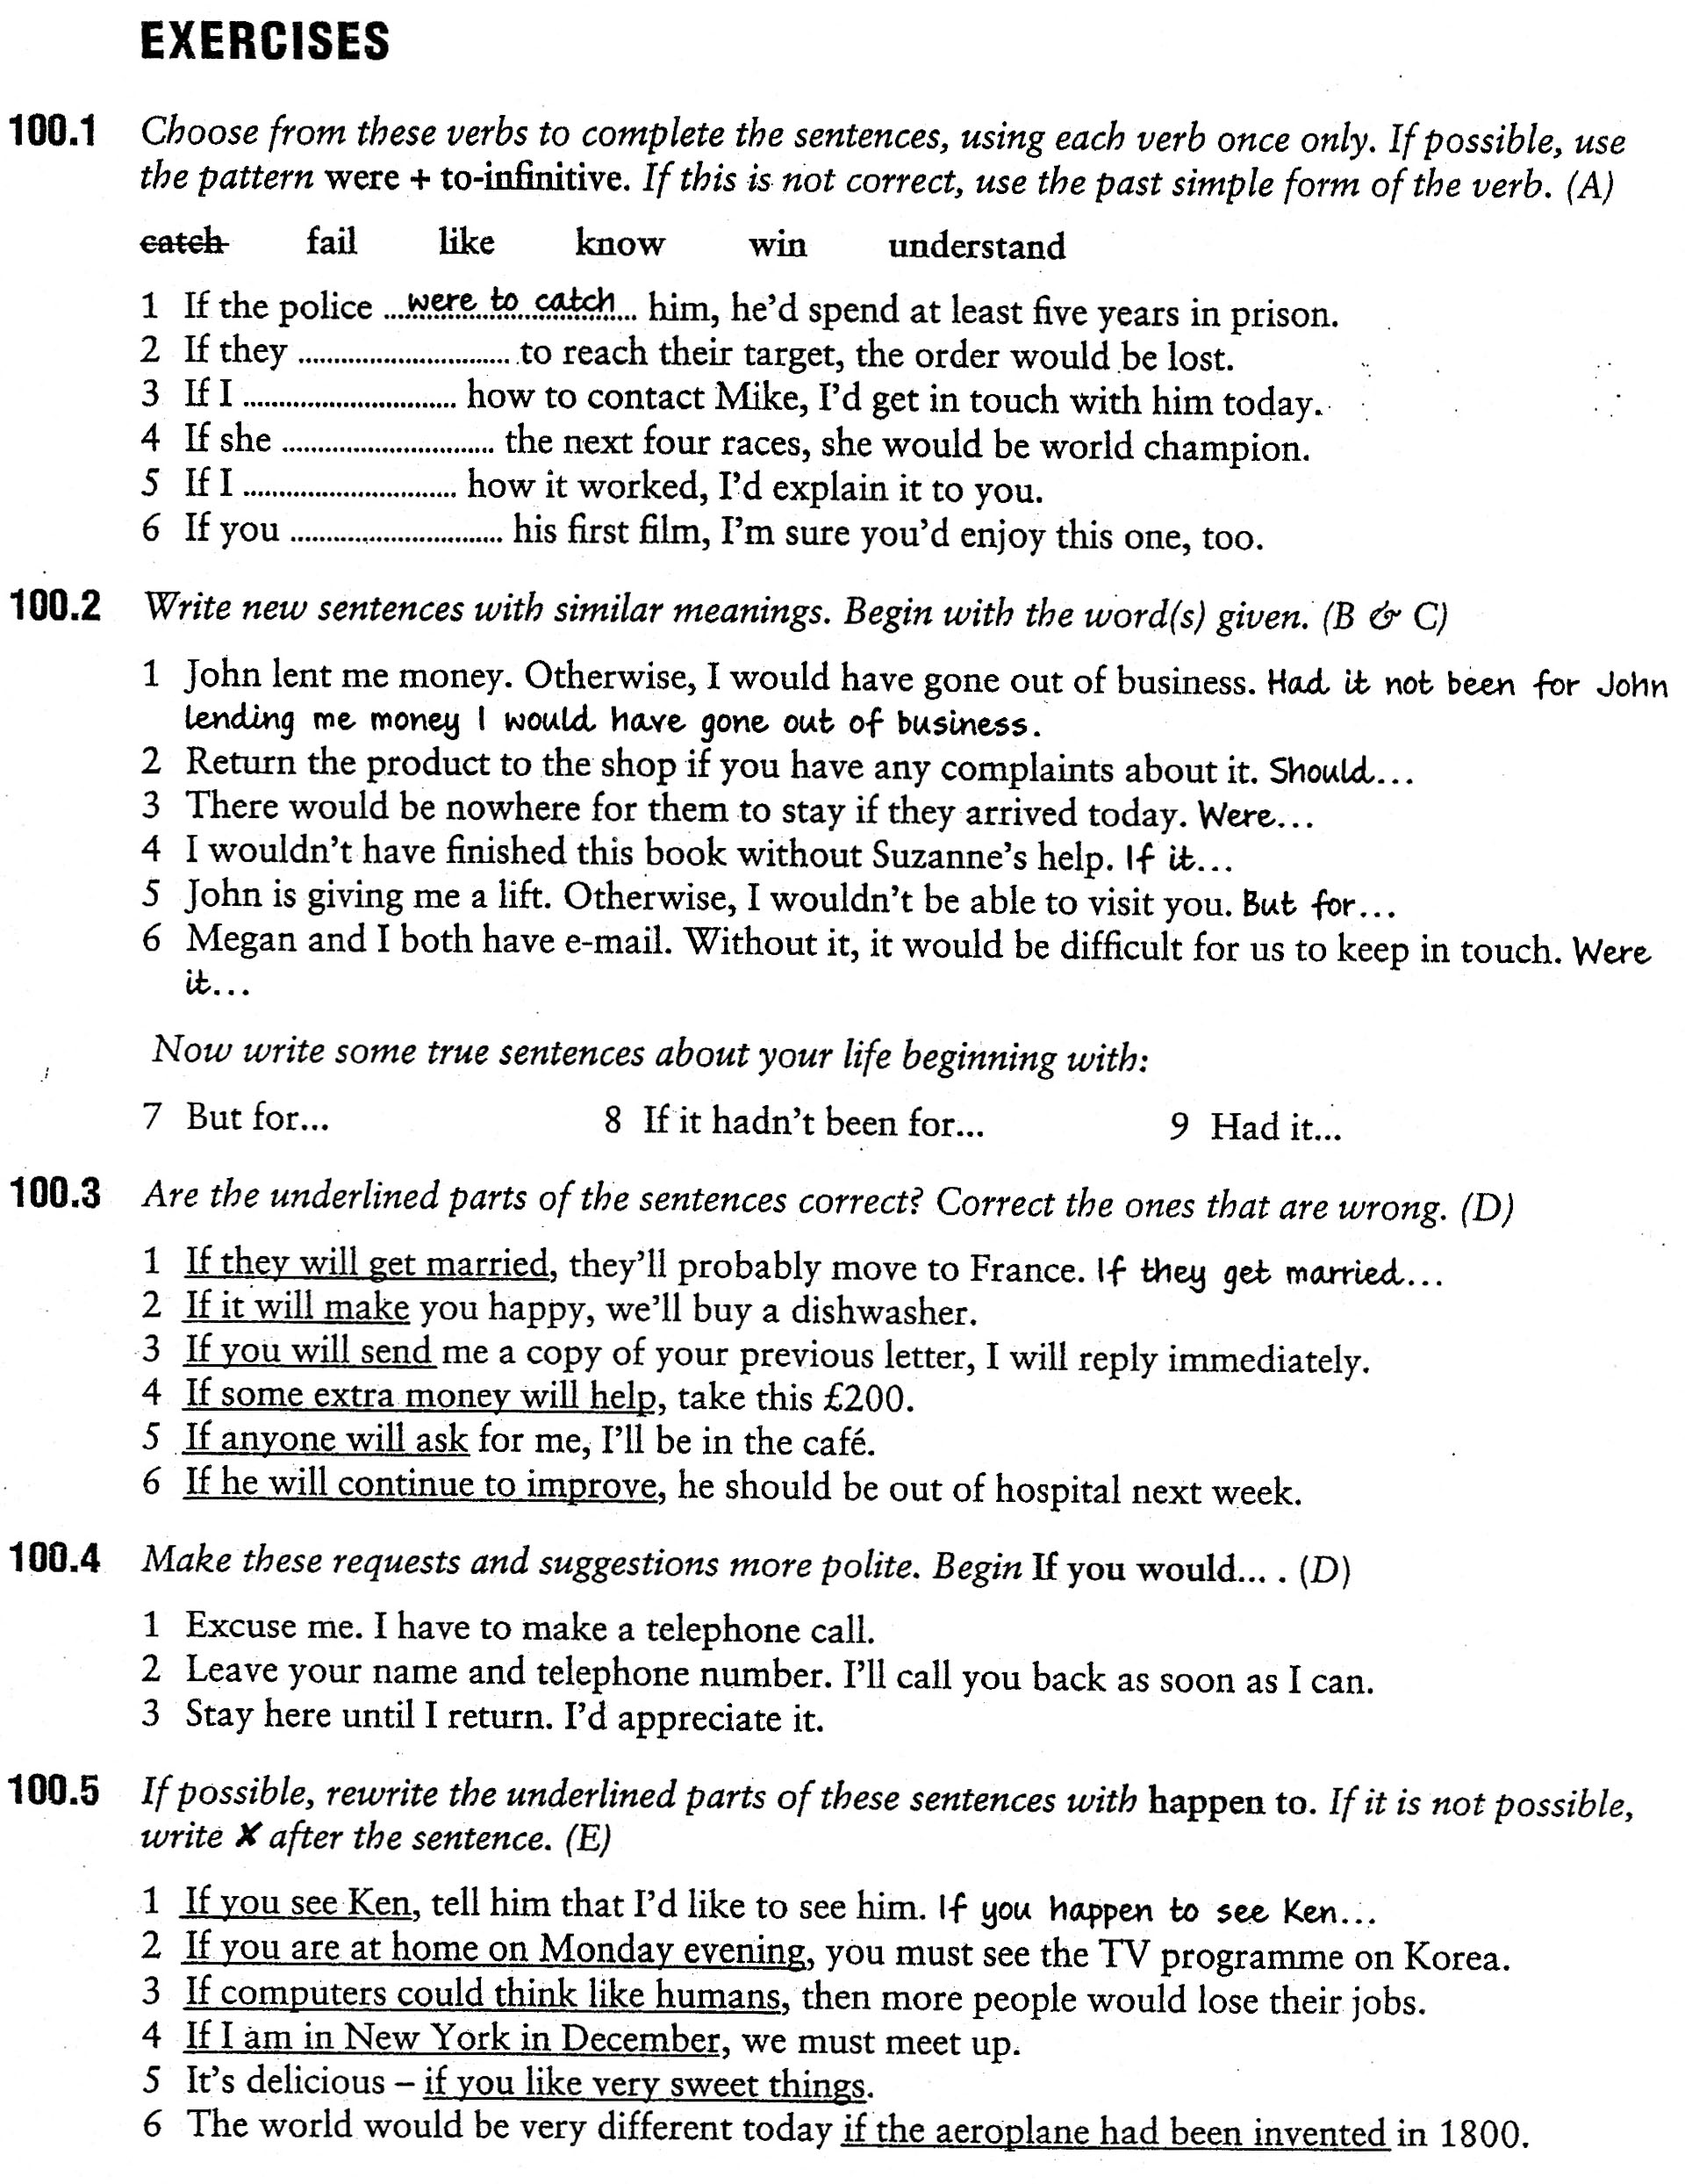
\includegraphics[scale=.85]{handouts/Eng109.jpg}

\chapter{Business Structures}
Business 21, ch. 3
\section{Legal forms of Doing Business in Germany}
%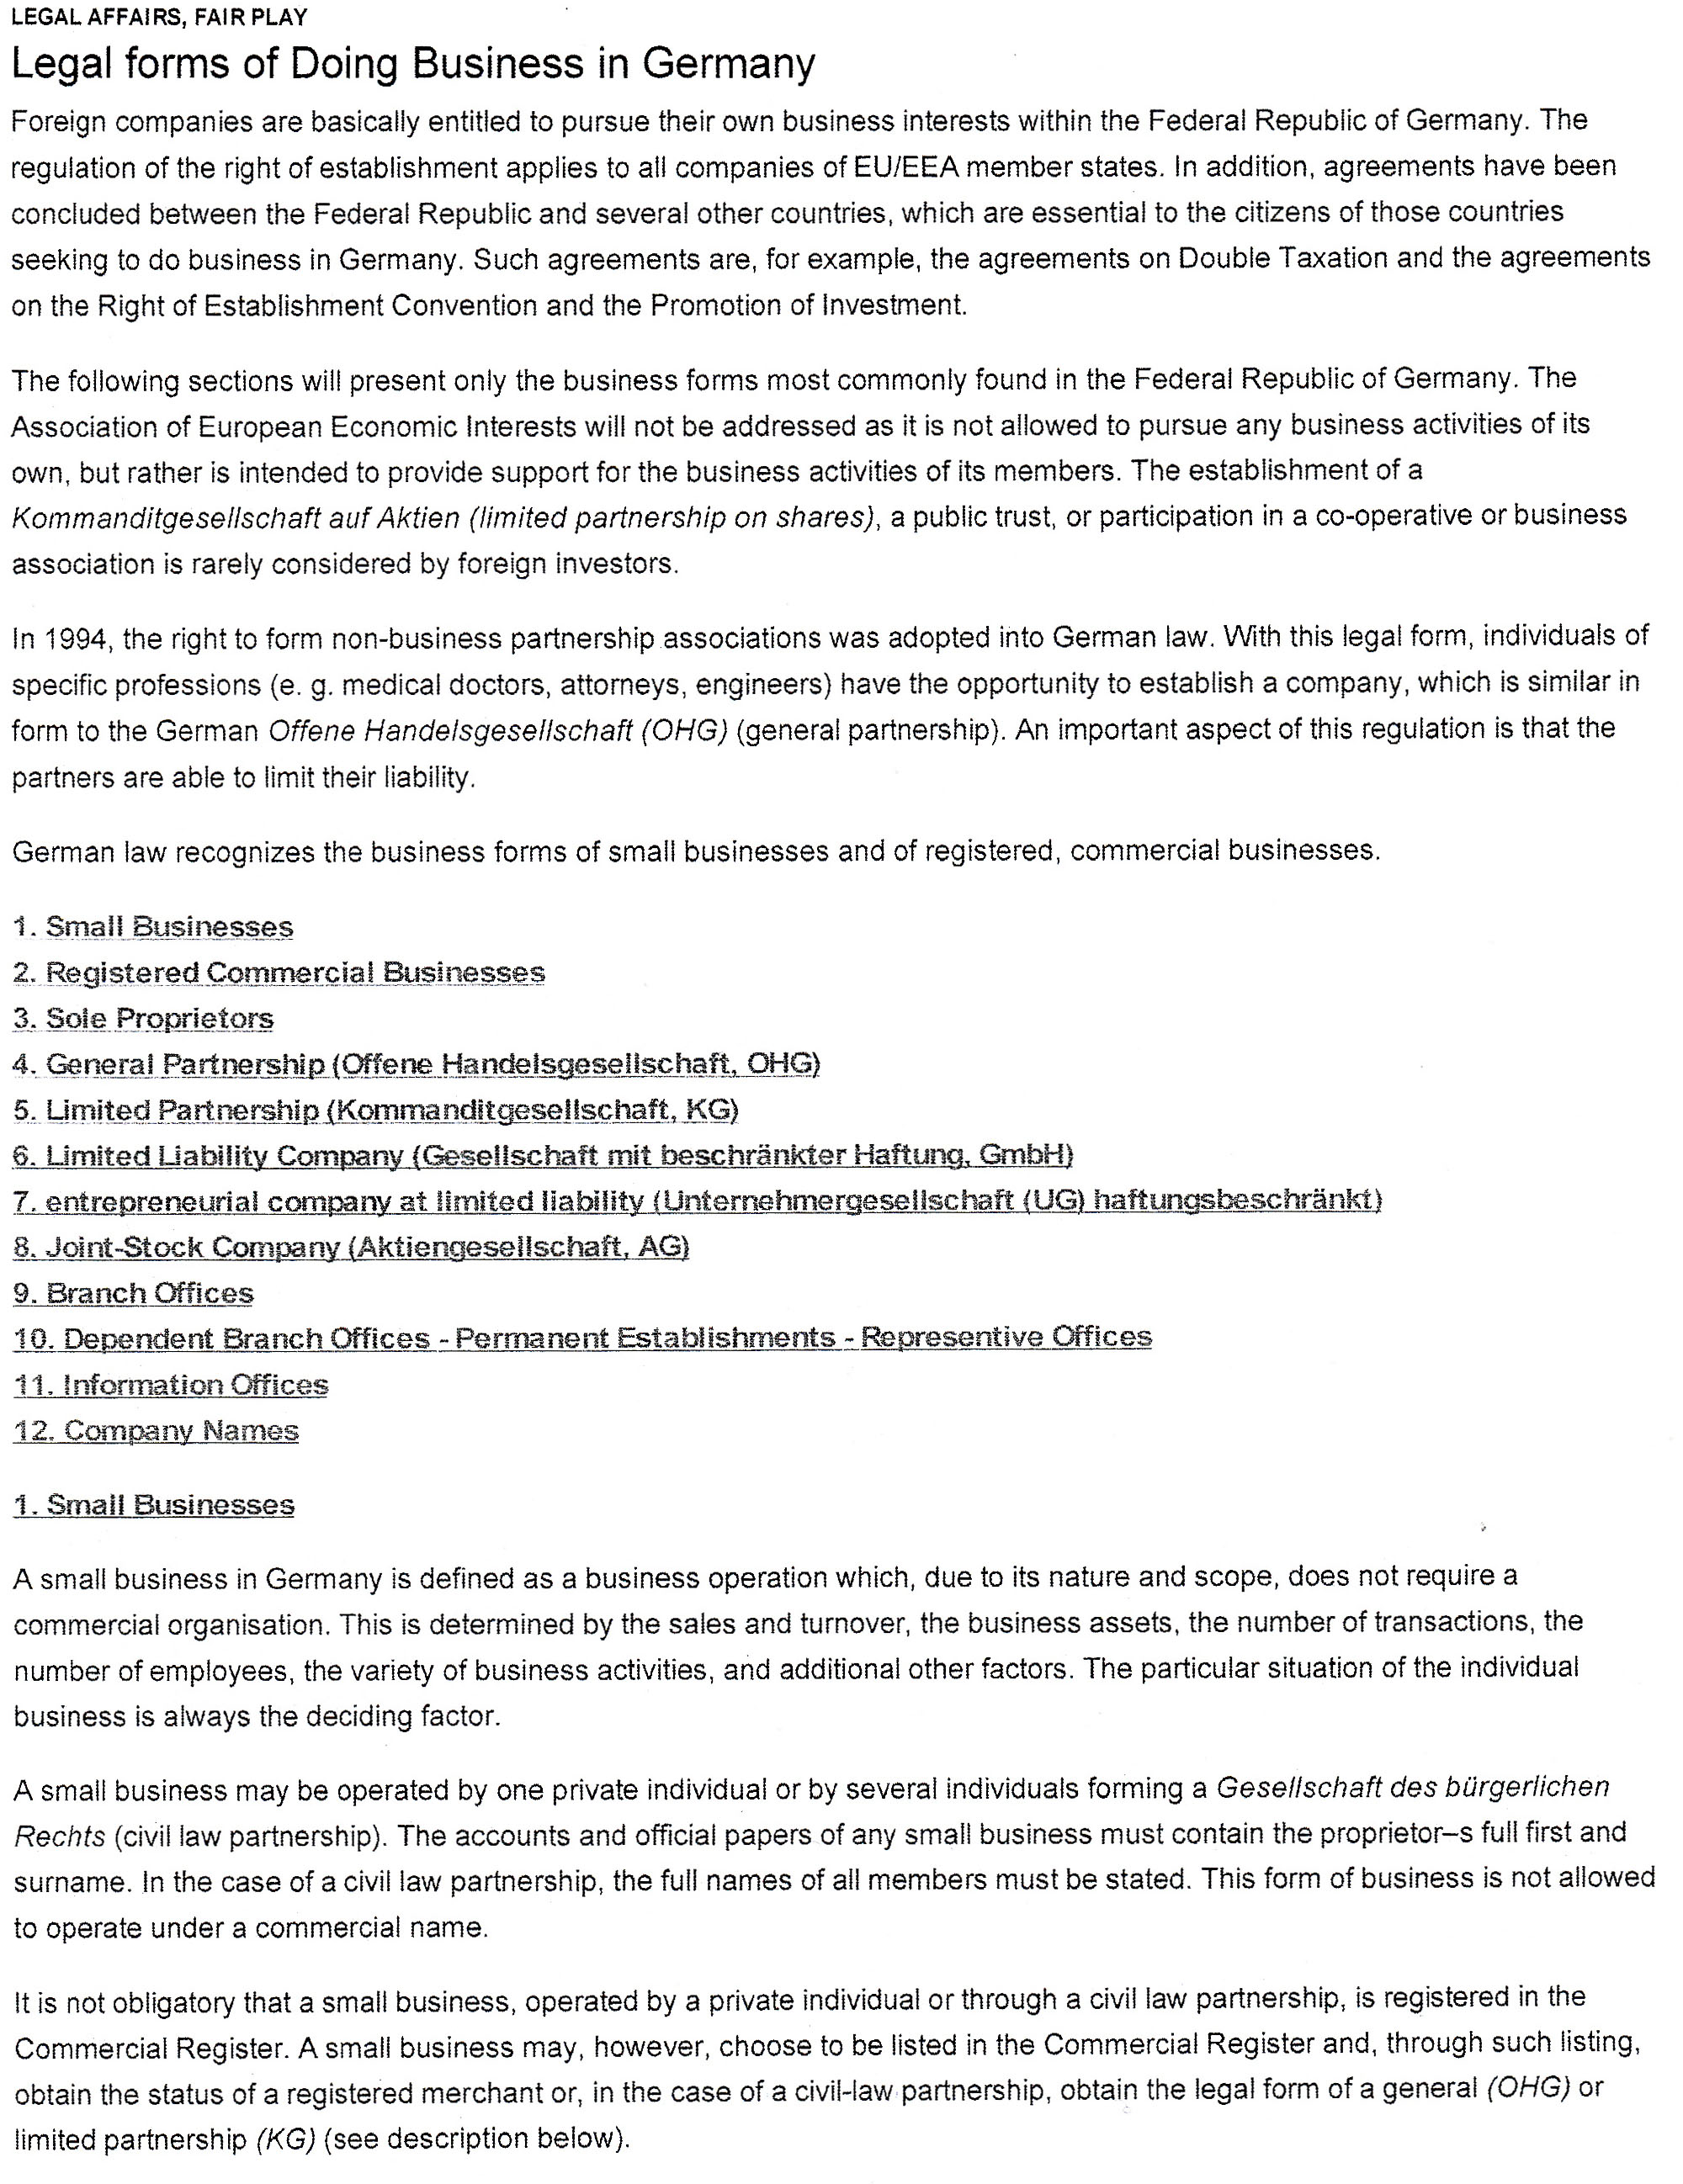
\includegraphics[scale=.85]{handouts/Eng201.jpg}

%
\includegraphics[scale=.85]{handouts/Eng202.jpg}

%
\includegraphics[scale=.85]{handouts/Eng203.jpg}

%
\includegraphics[scale=.85]{handouts/Eng204.jpg}
\section{What is Management?}
%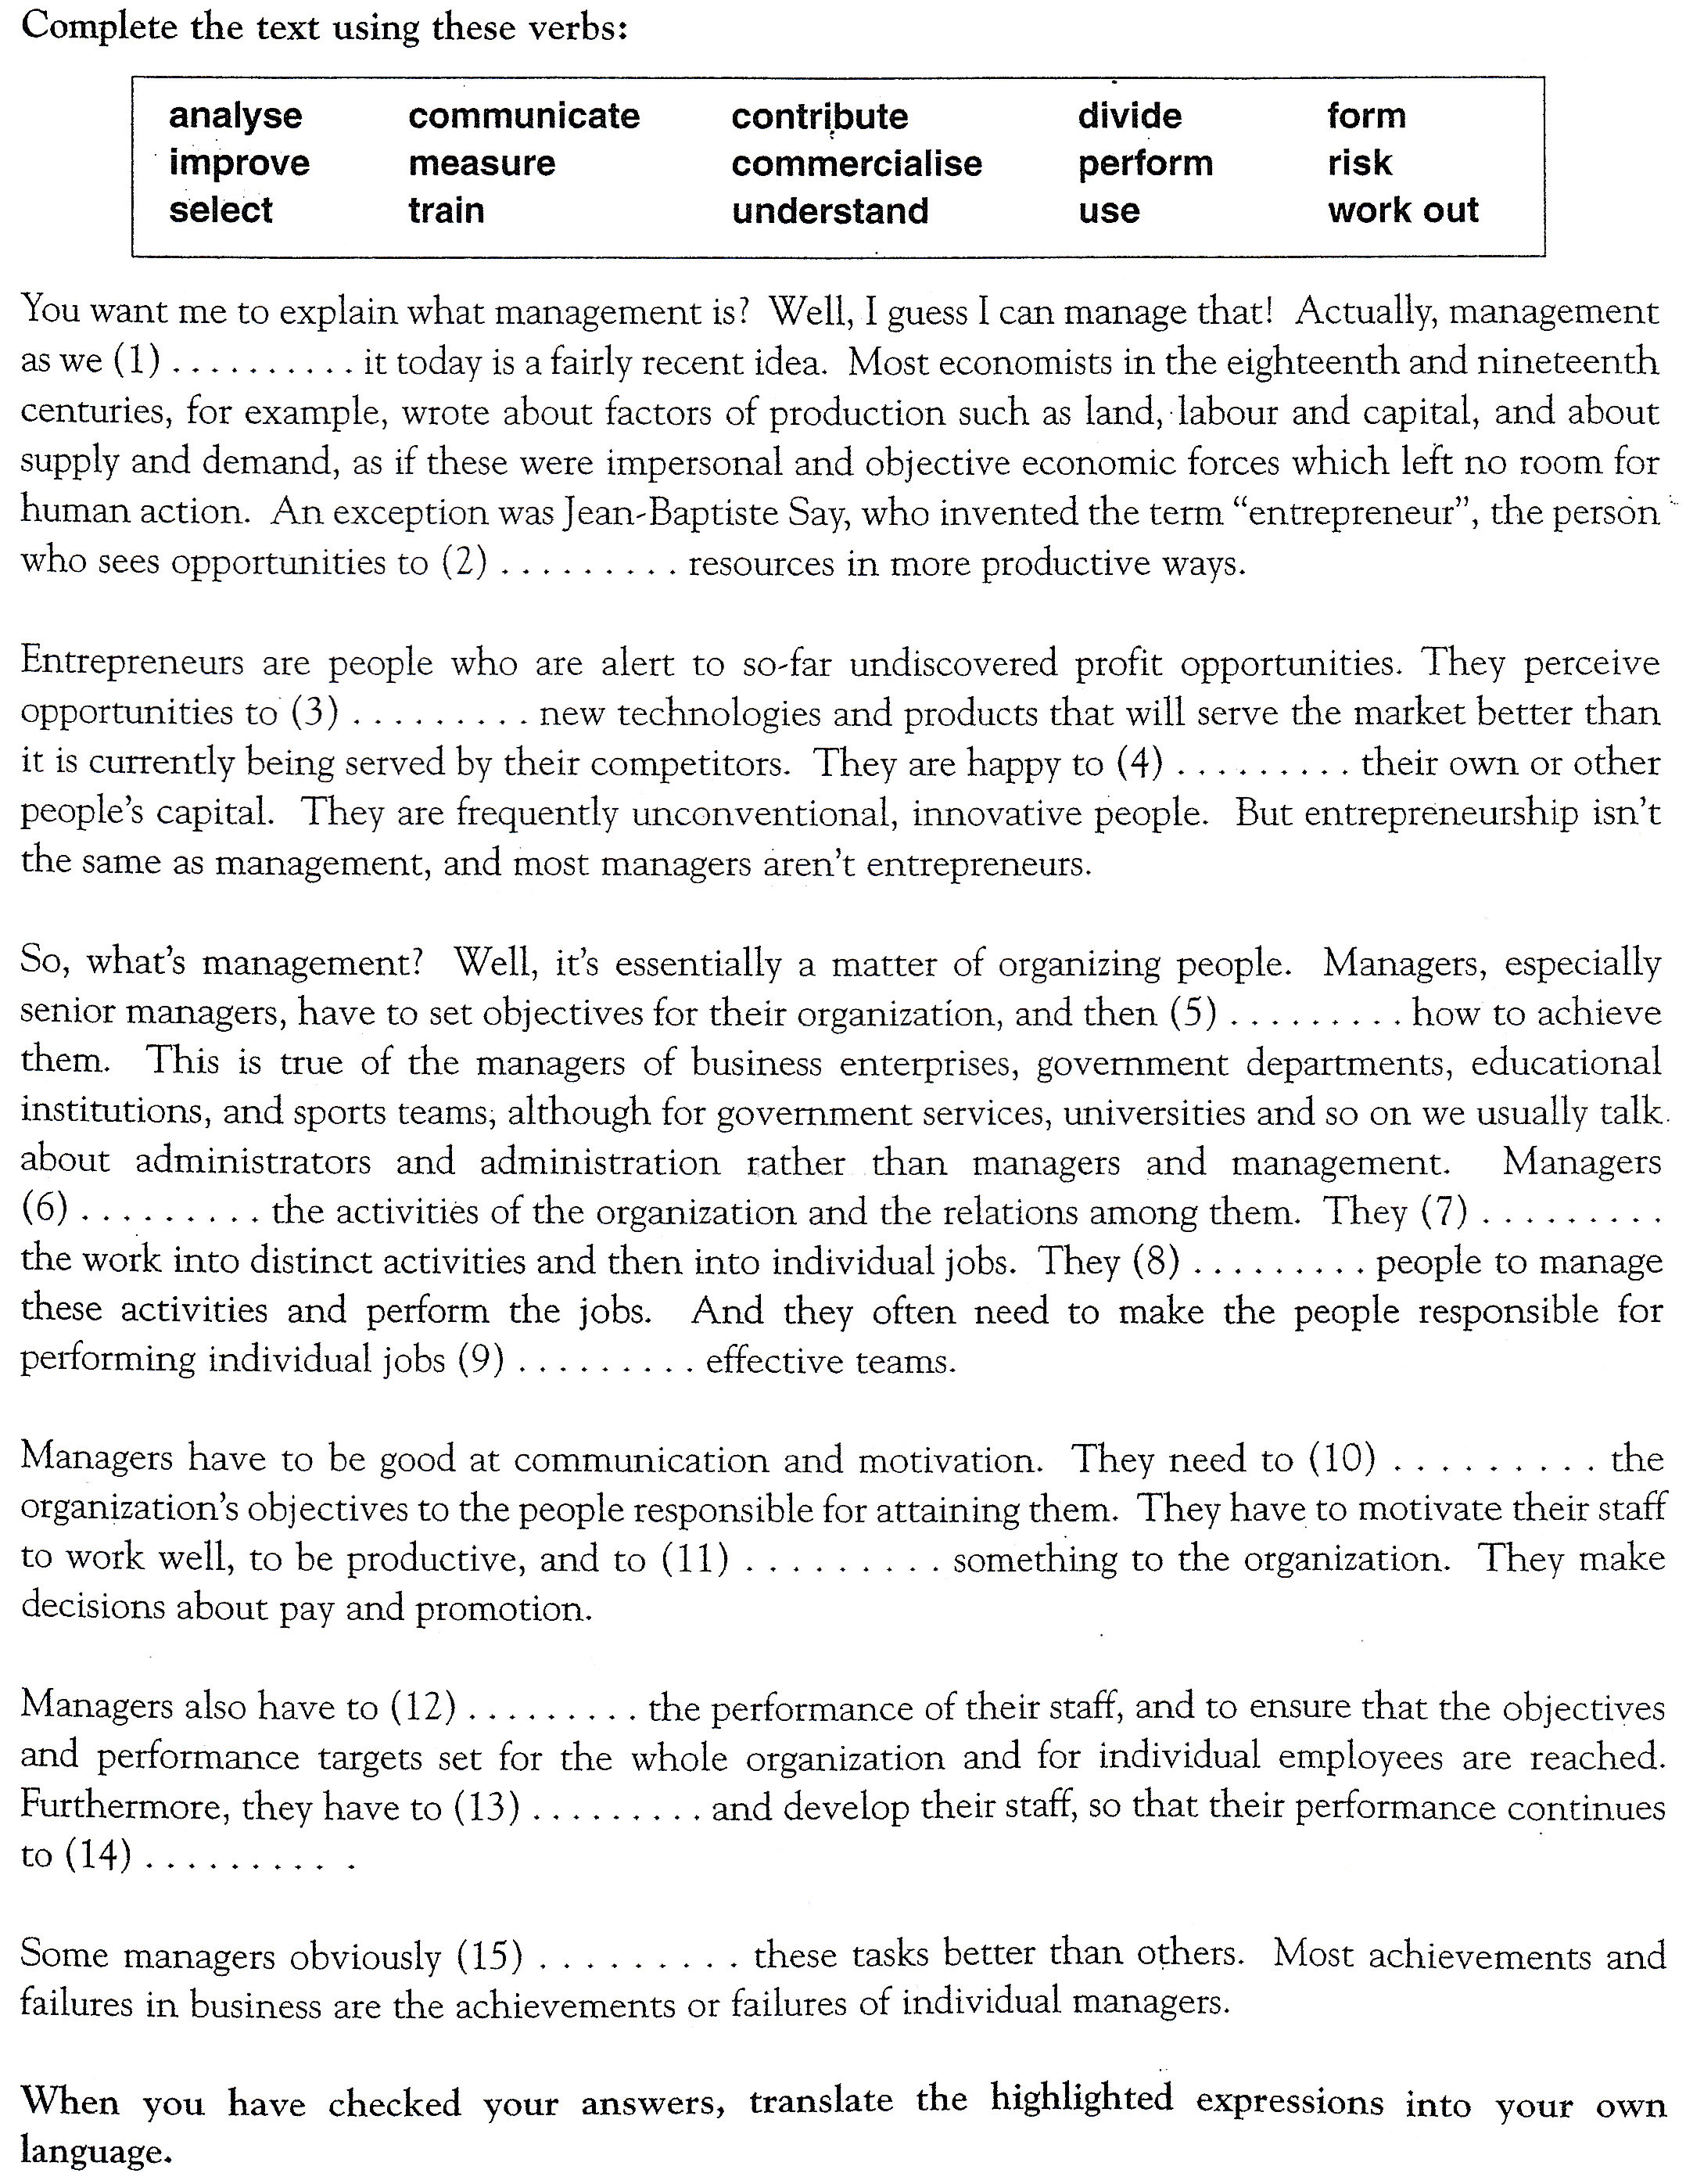
\includegraphics[scale=.85]{handouts/Eng205.jpg}
\section{Management Skills}
%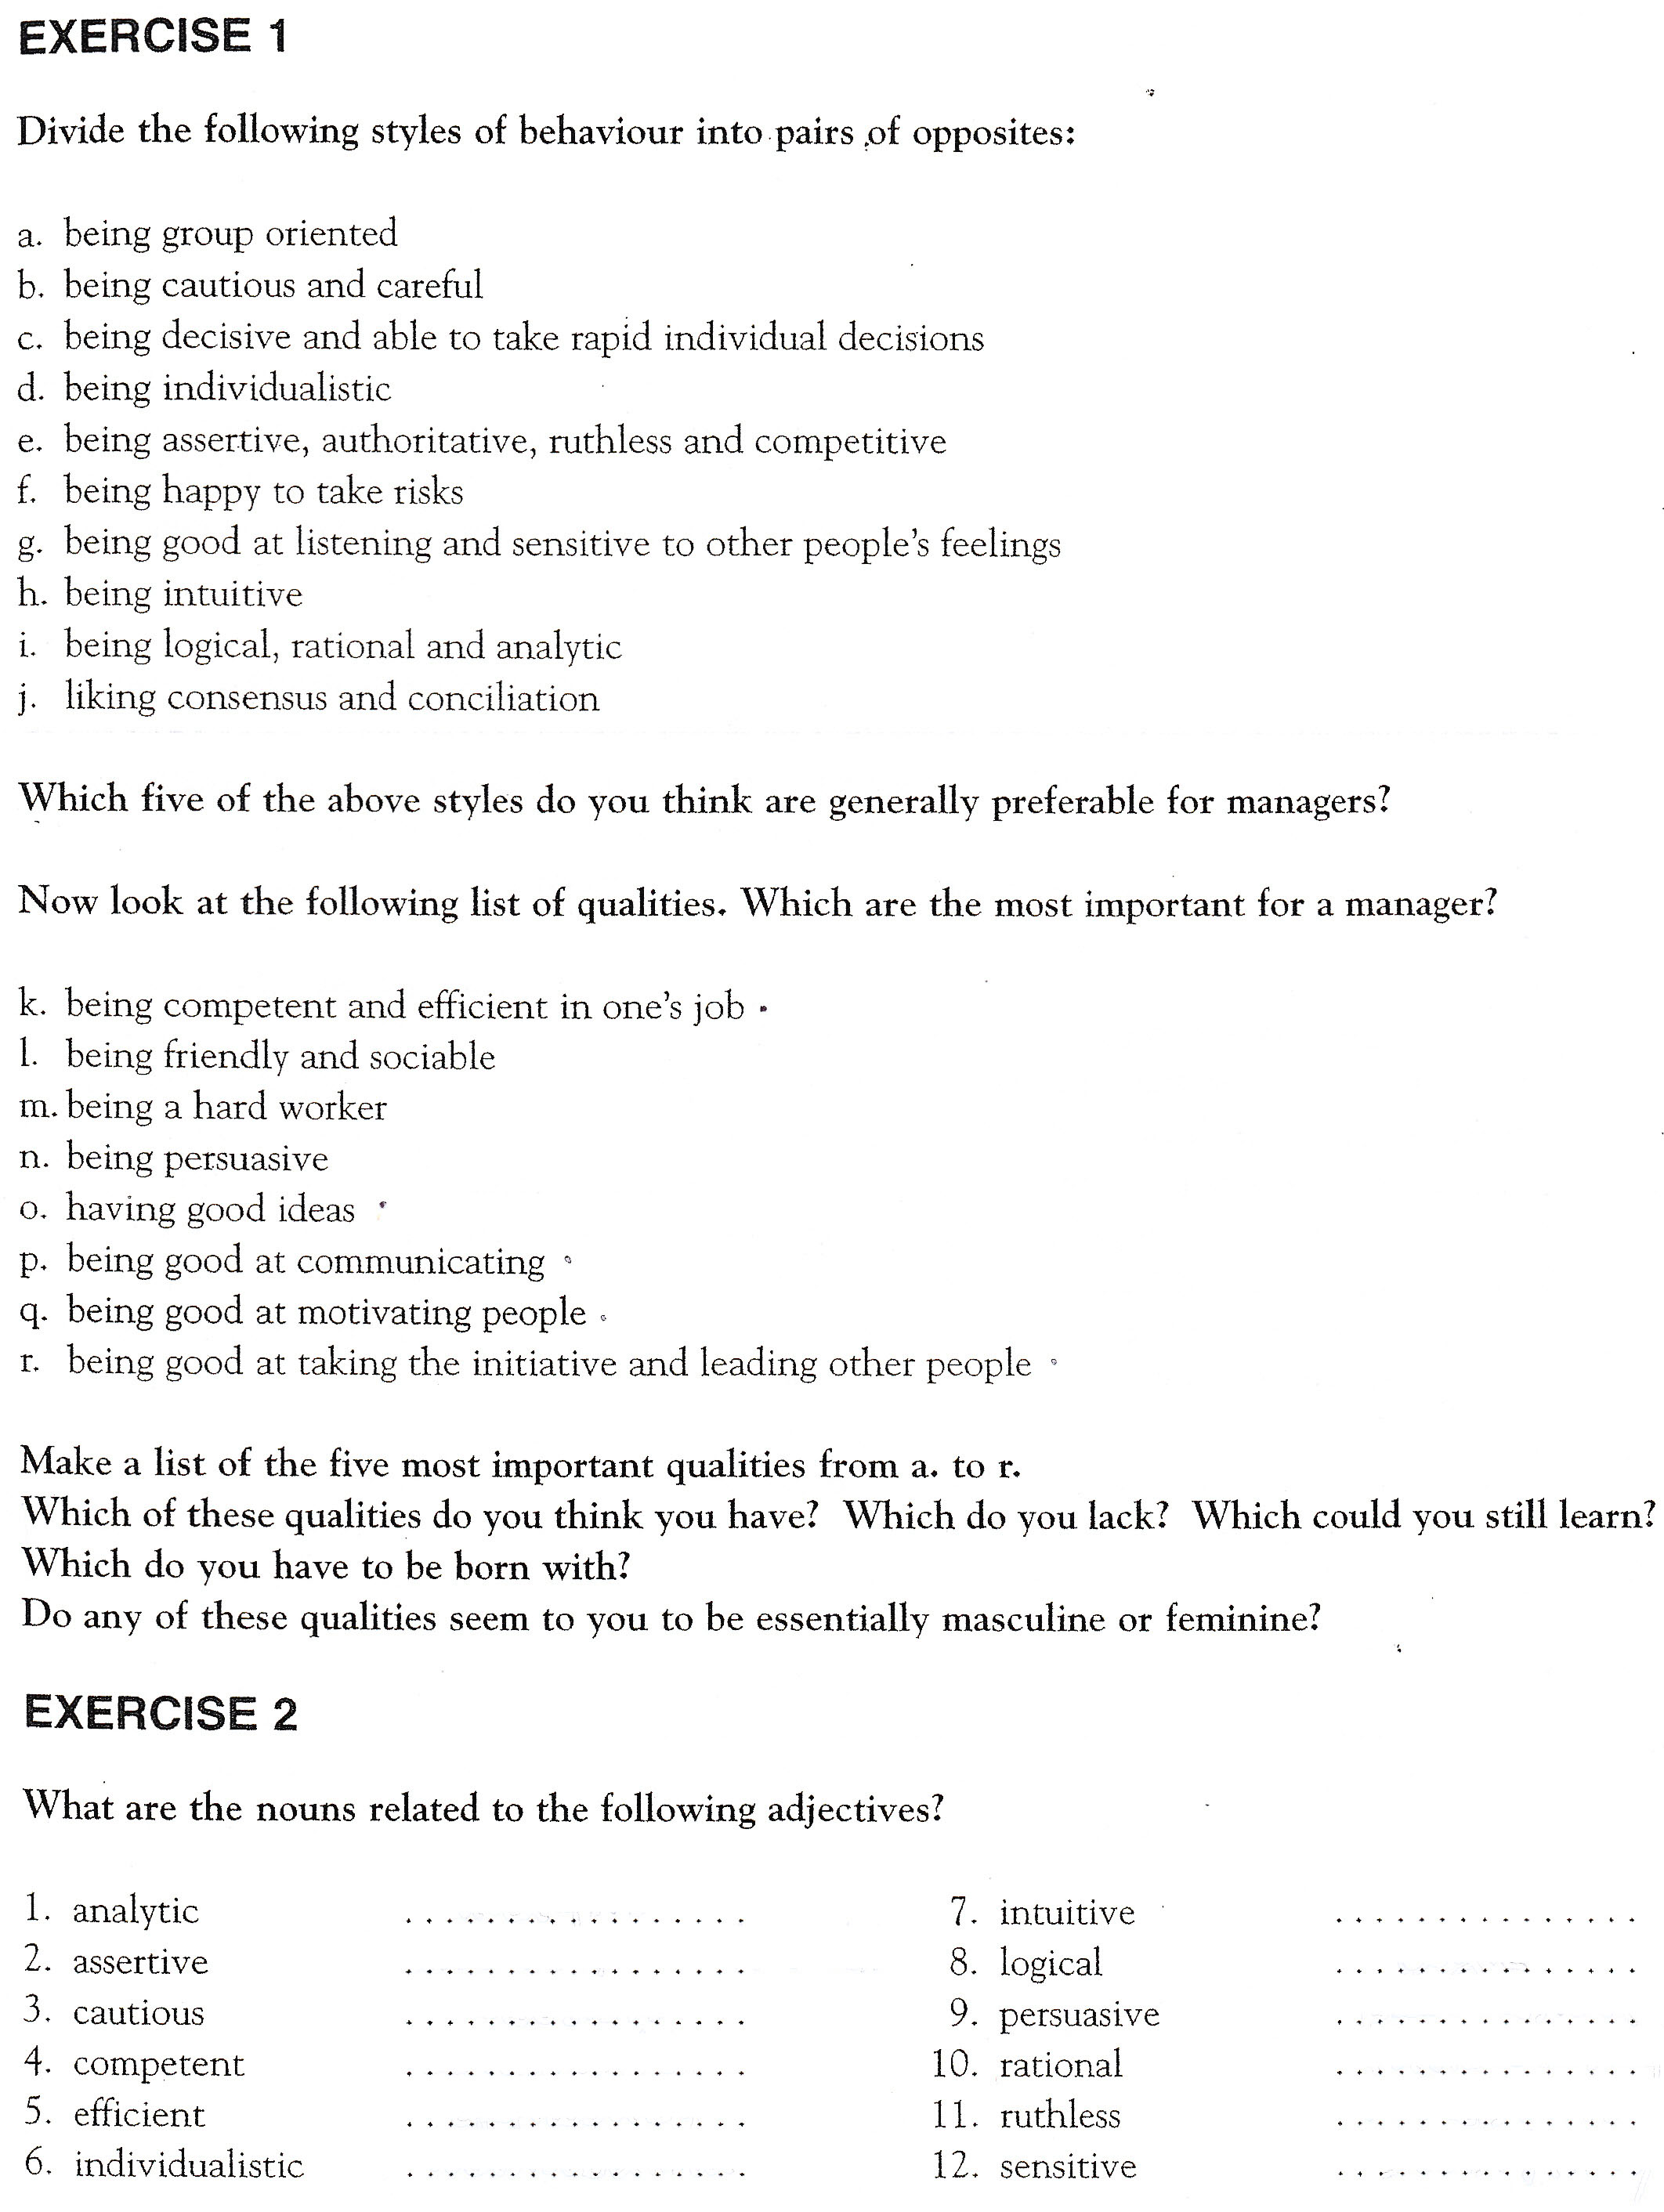
\includegraphics[scale=.85]{handouts/Eng206.jpg}
\section{Company Structure}
%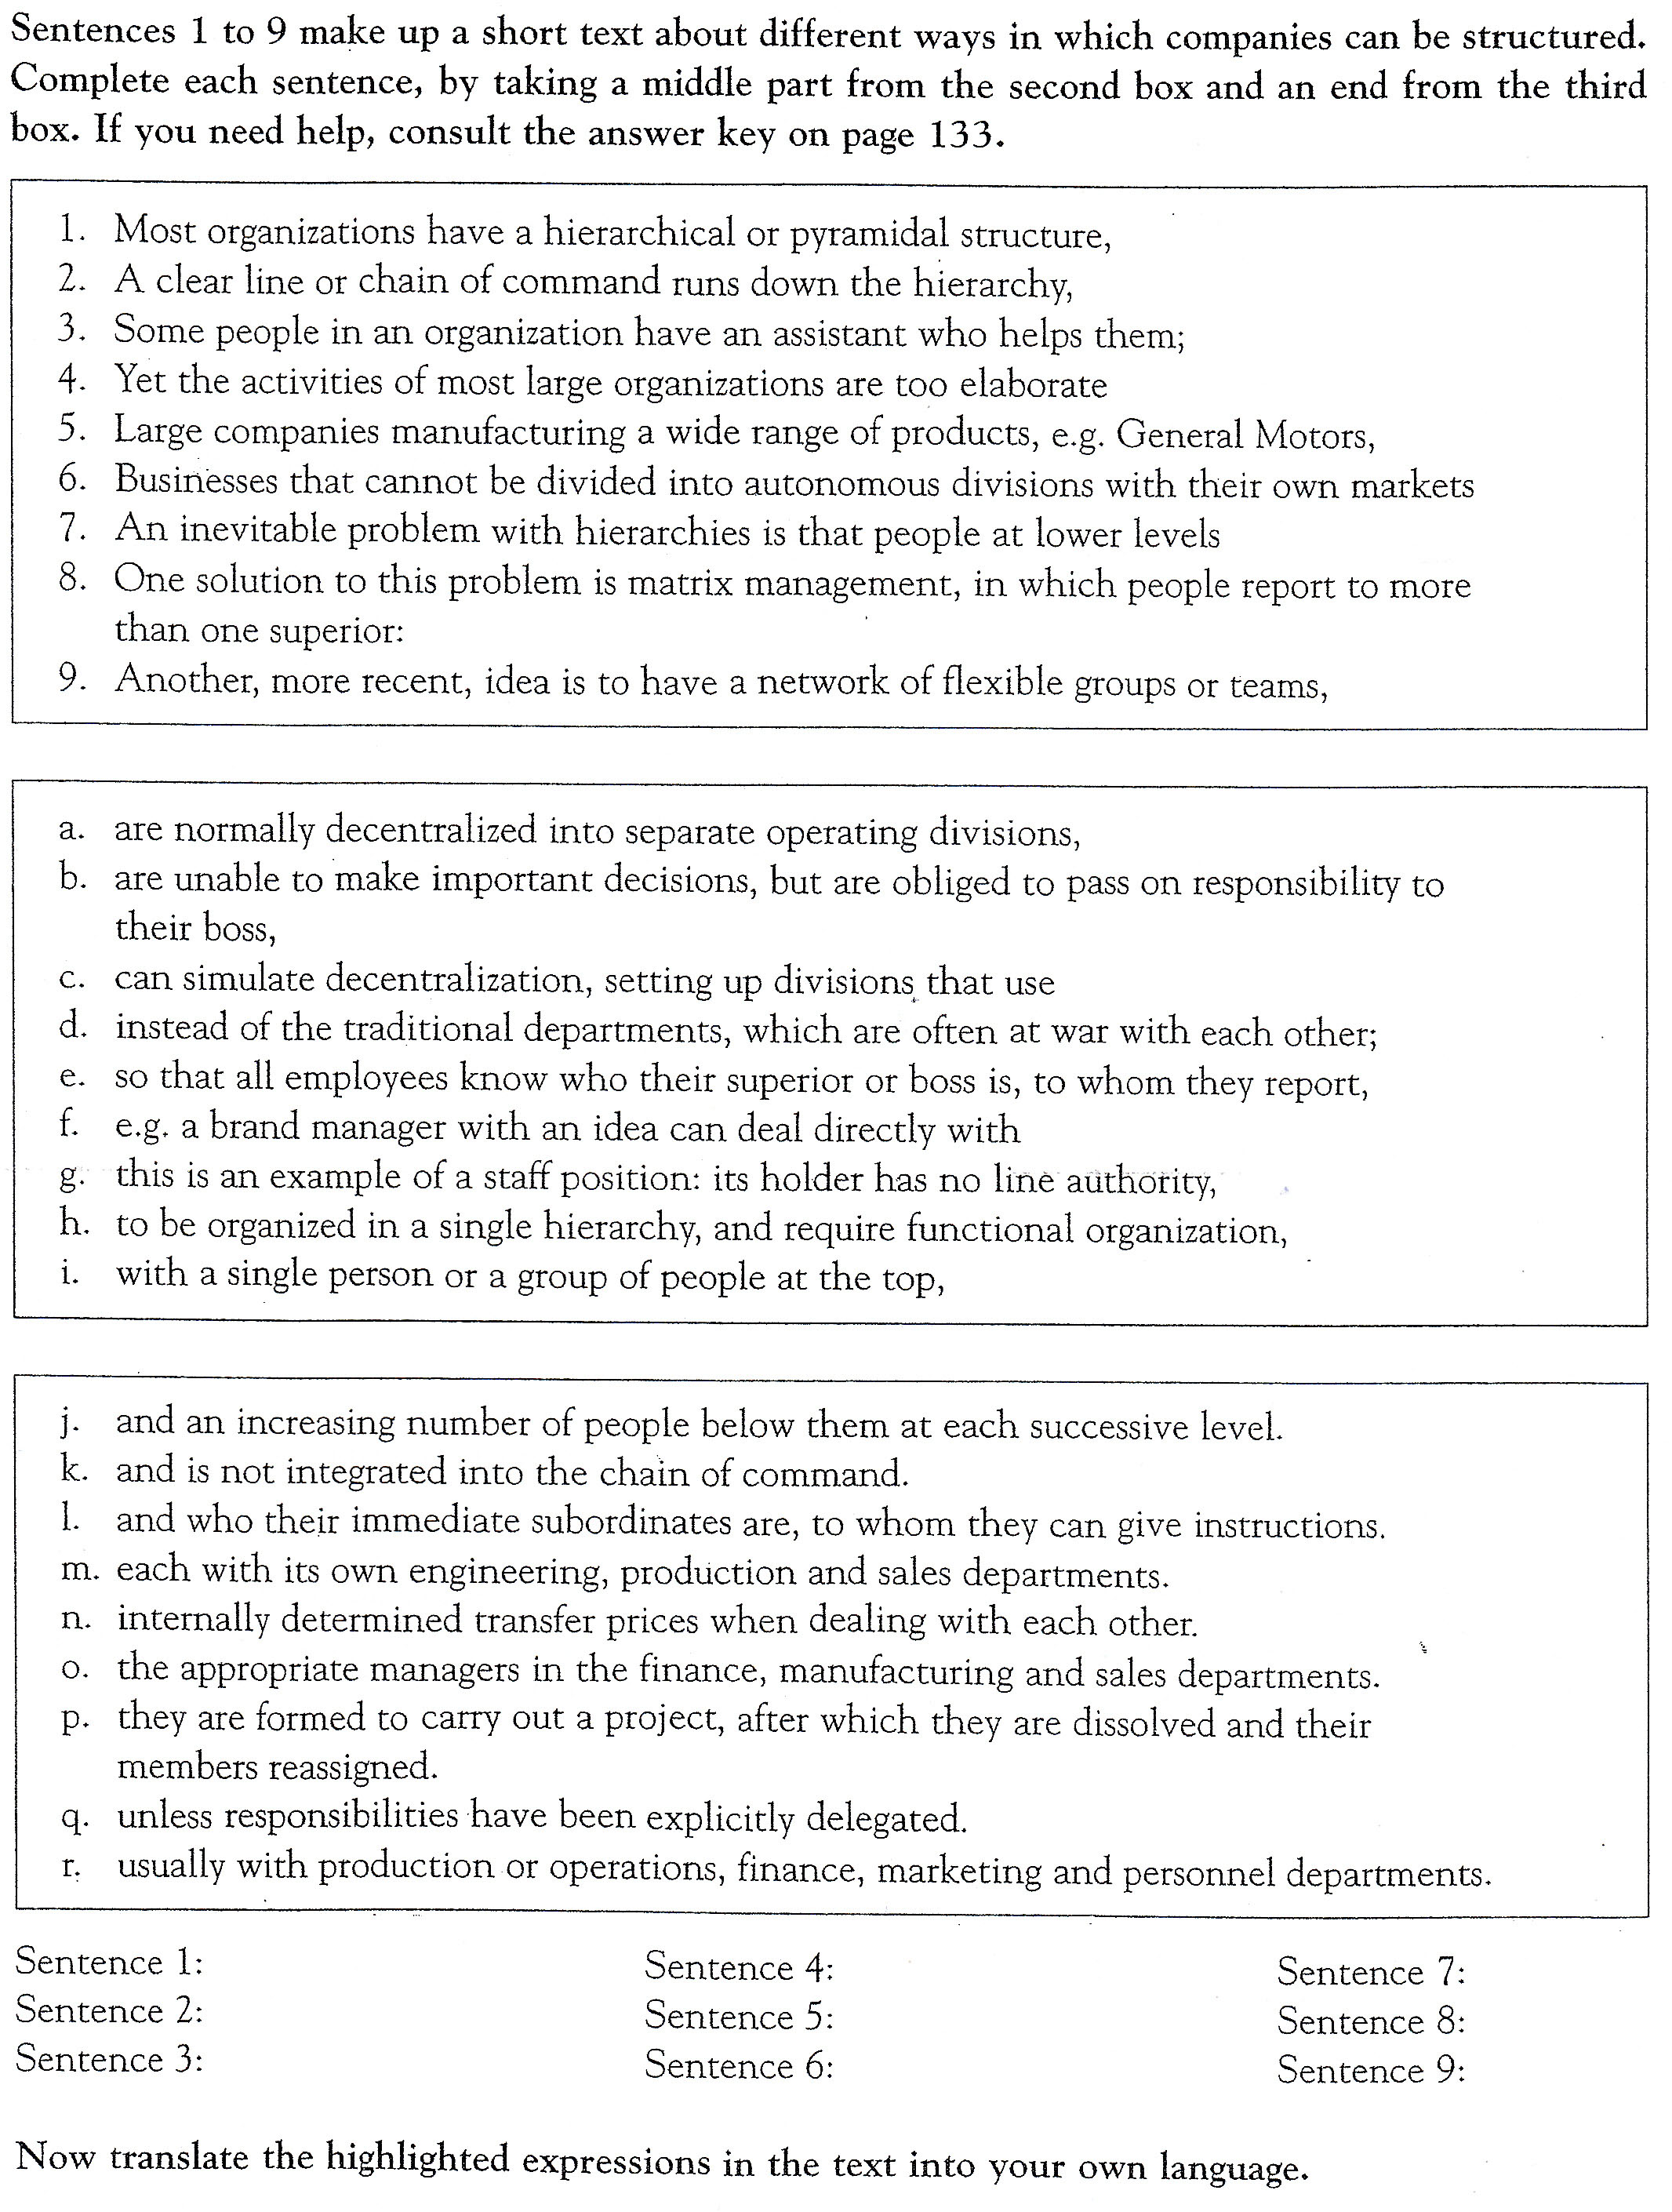
\includegraphics[scale=.85]{handouts/Eng207.jpg}
\section{An Organization Chart}
%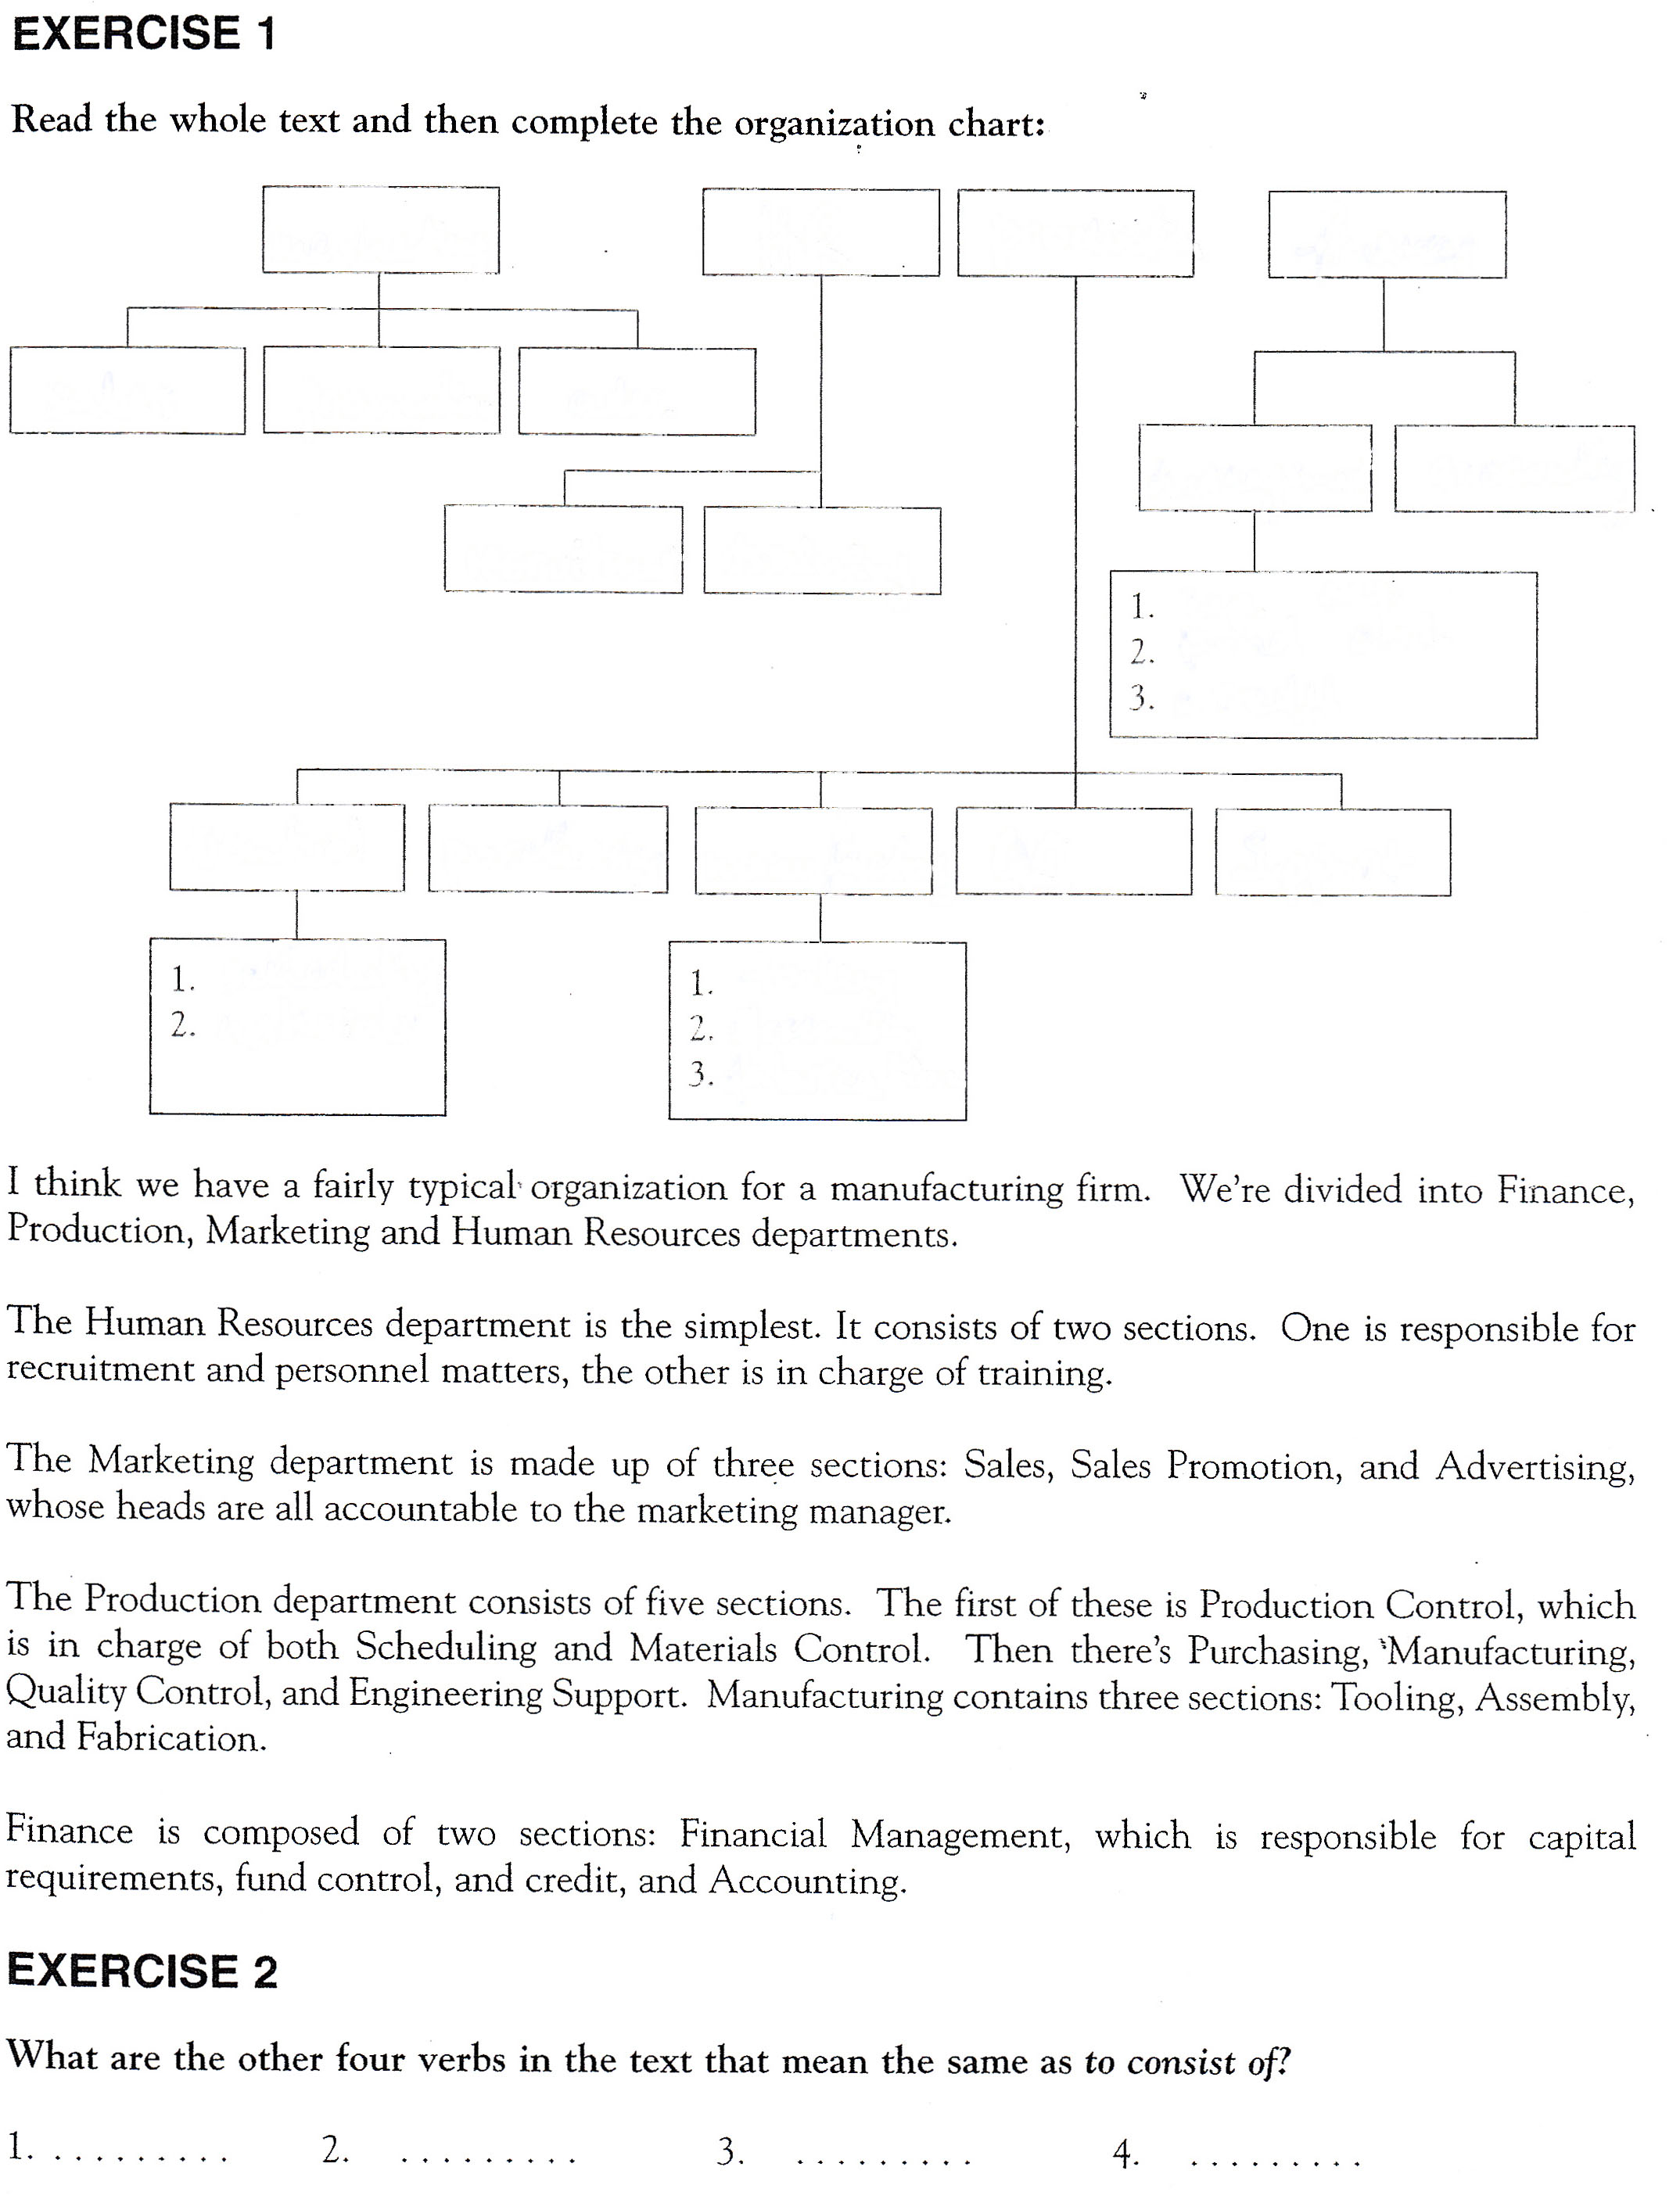
\includegraphics[scale=.85]{handouts/Eng208.jpg}
\section{Self-Study}
%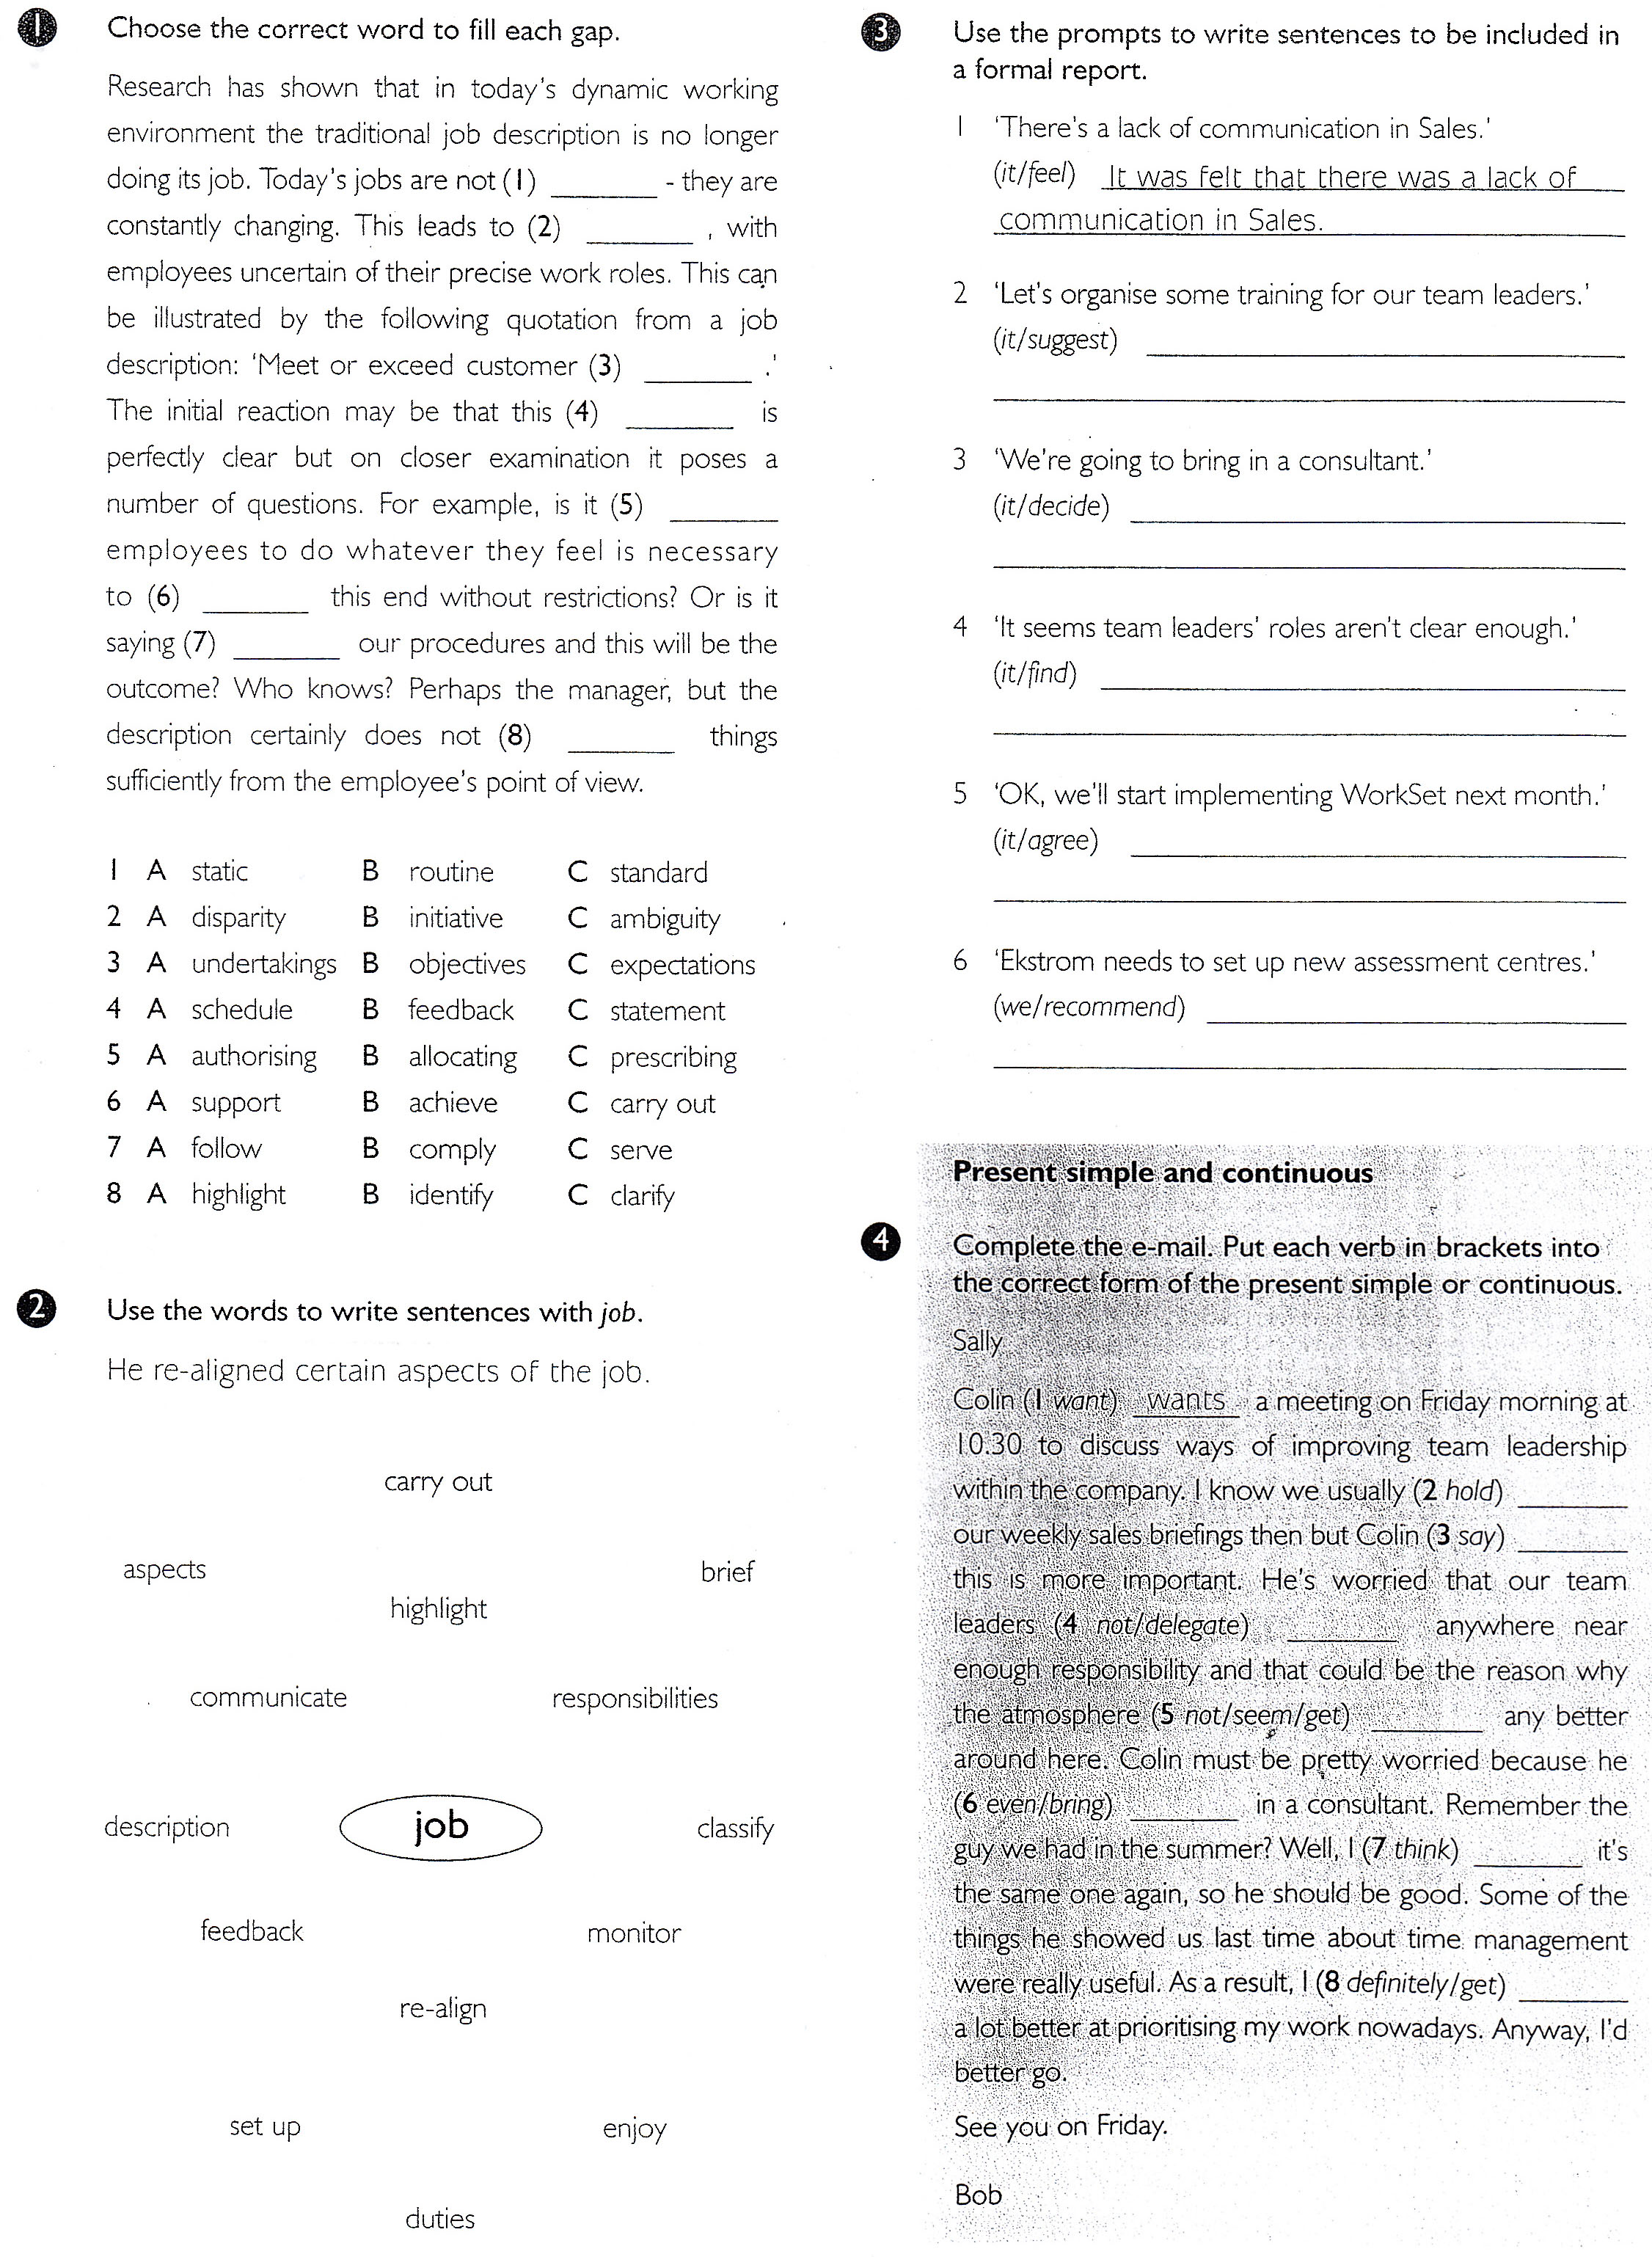
\includegraphics[scale=.85]{handouts/Eng209.jpg}

%\chapter{Career Express}
%Career Express B2: Unit 2 pp. 16-19\\
%C1: Unit 6 pp.56-59

\chapter{Personal Development}
Success with BEC: Unit 1.1, pp 6-8\\
The Business Advanced: Unit 1 Pers. Development, pp 8-9, 14-15
\section{Grammar}
%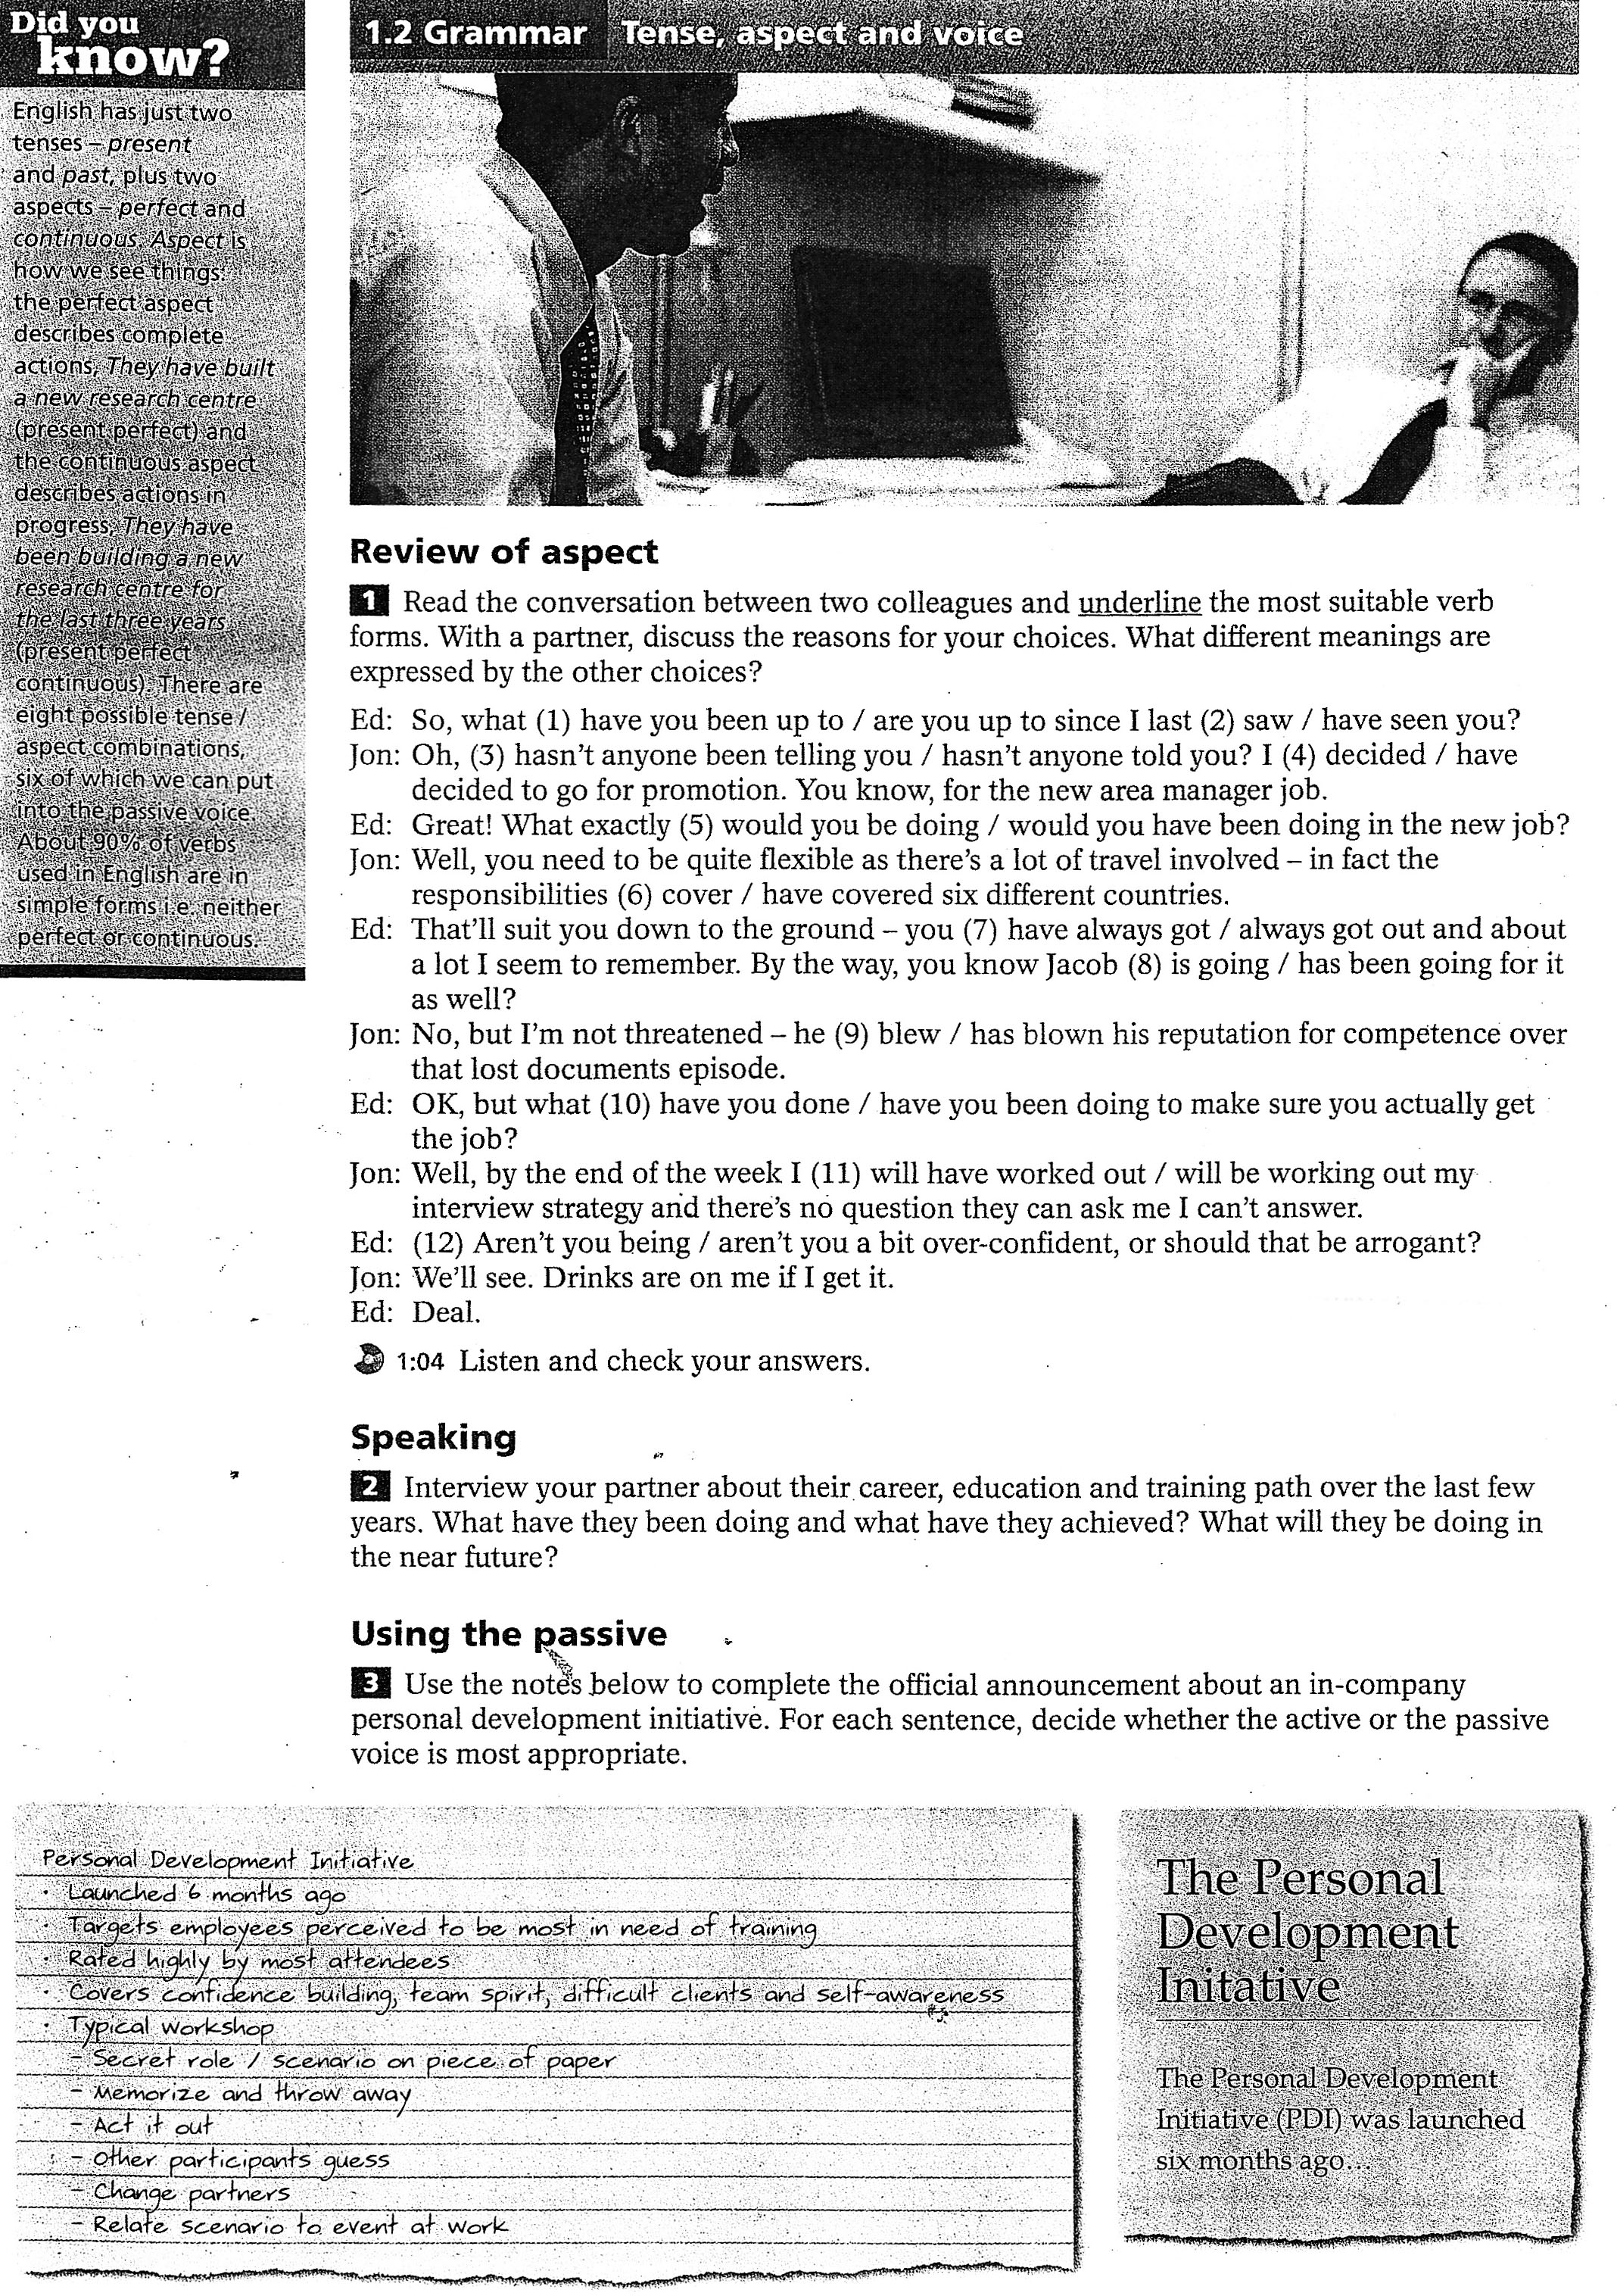
\includegraphics[scale=.85]{handouts/Eng301.jpg}

%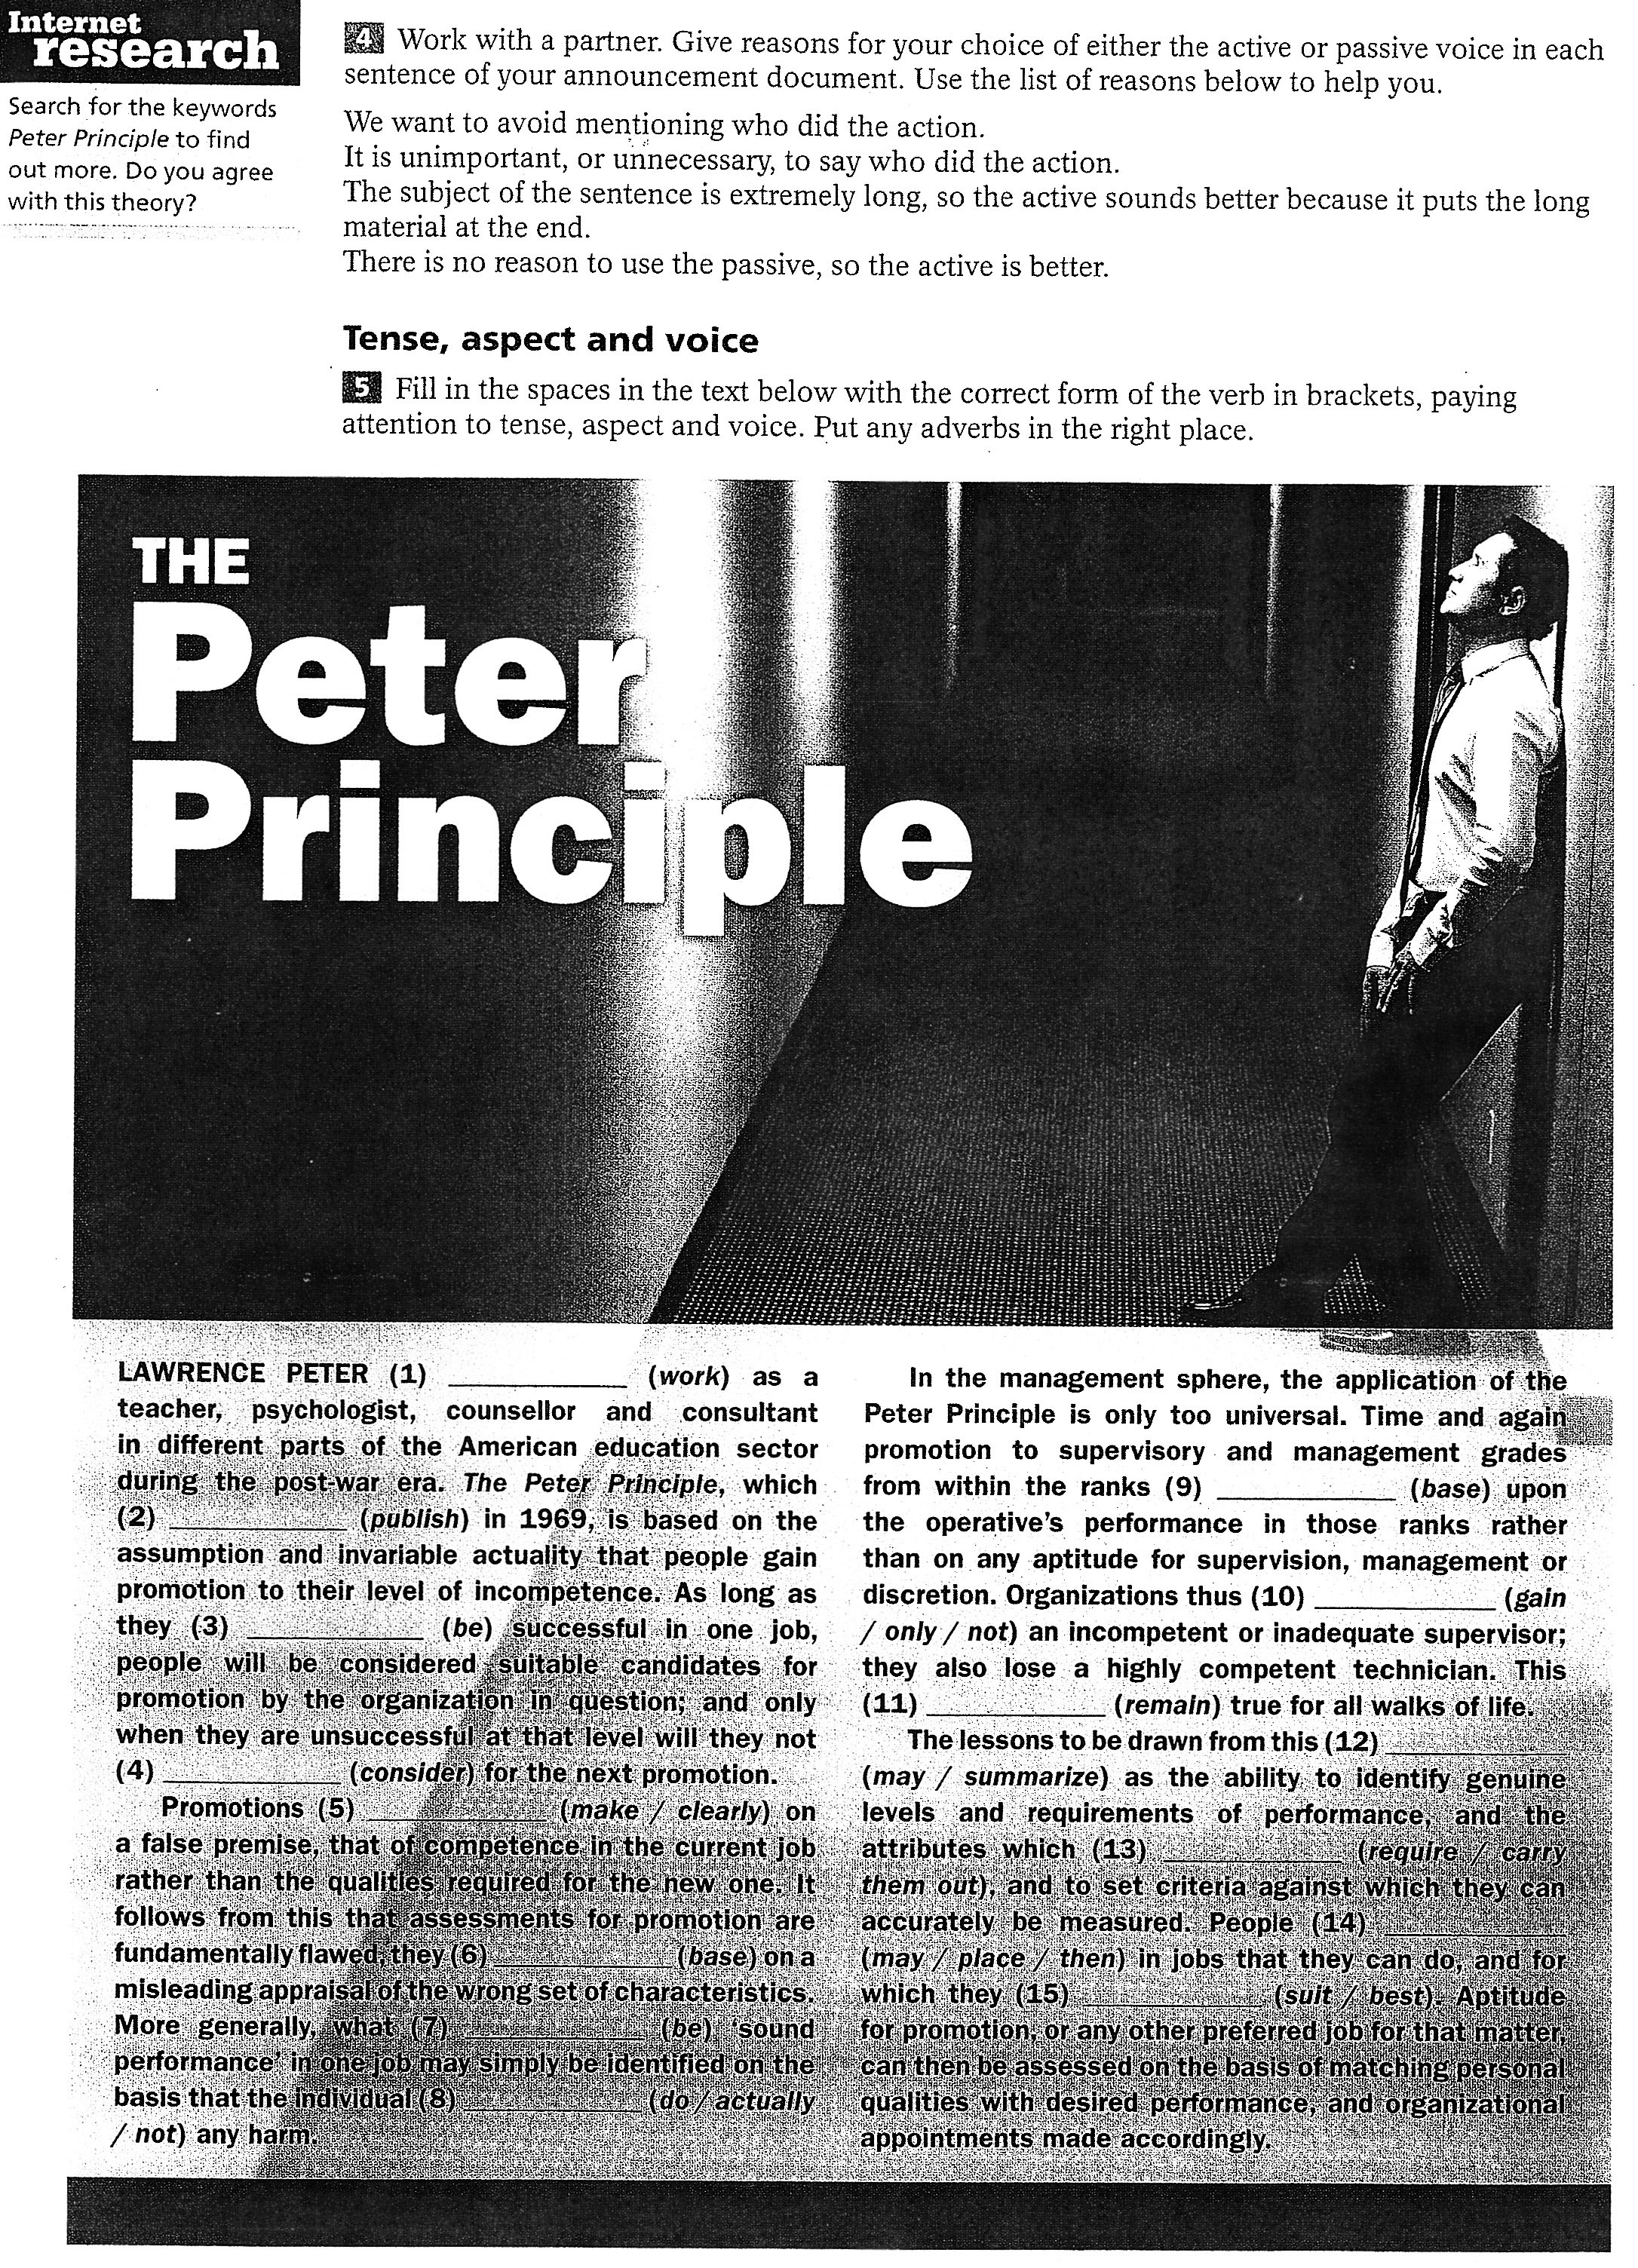
\includegraphics[scale=.85]{handouts/Eng302.jpg}
\section{Vocabulary}
%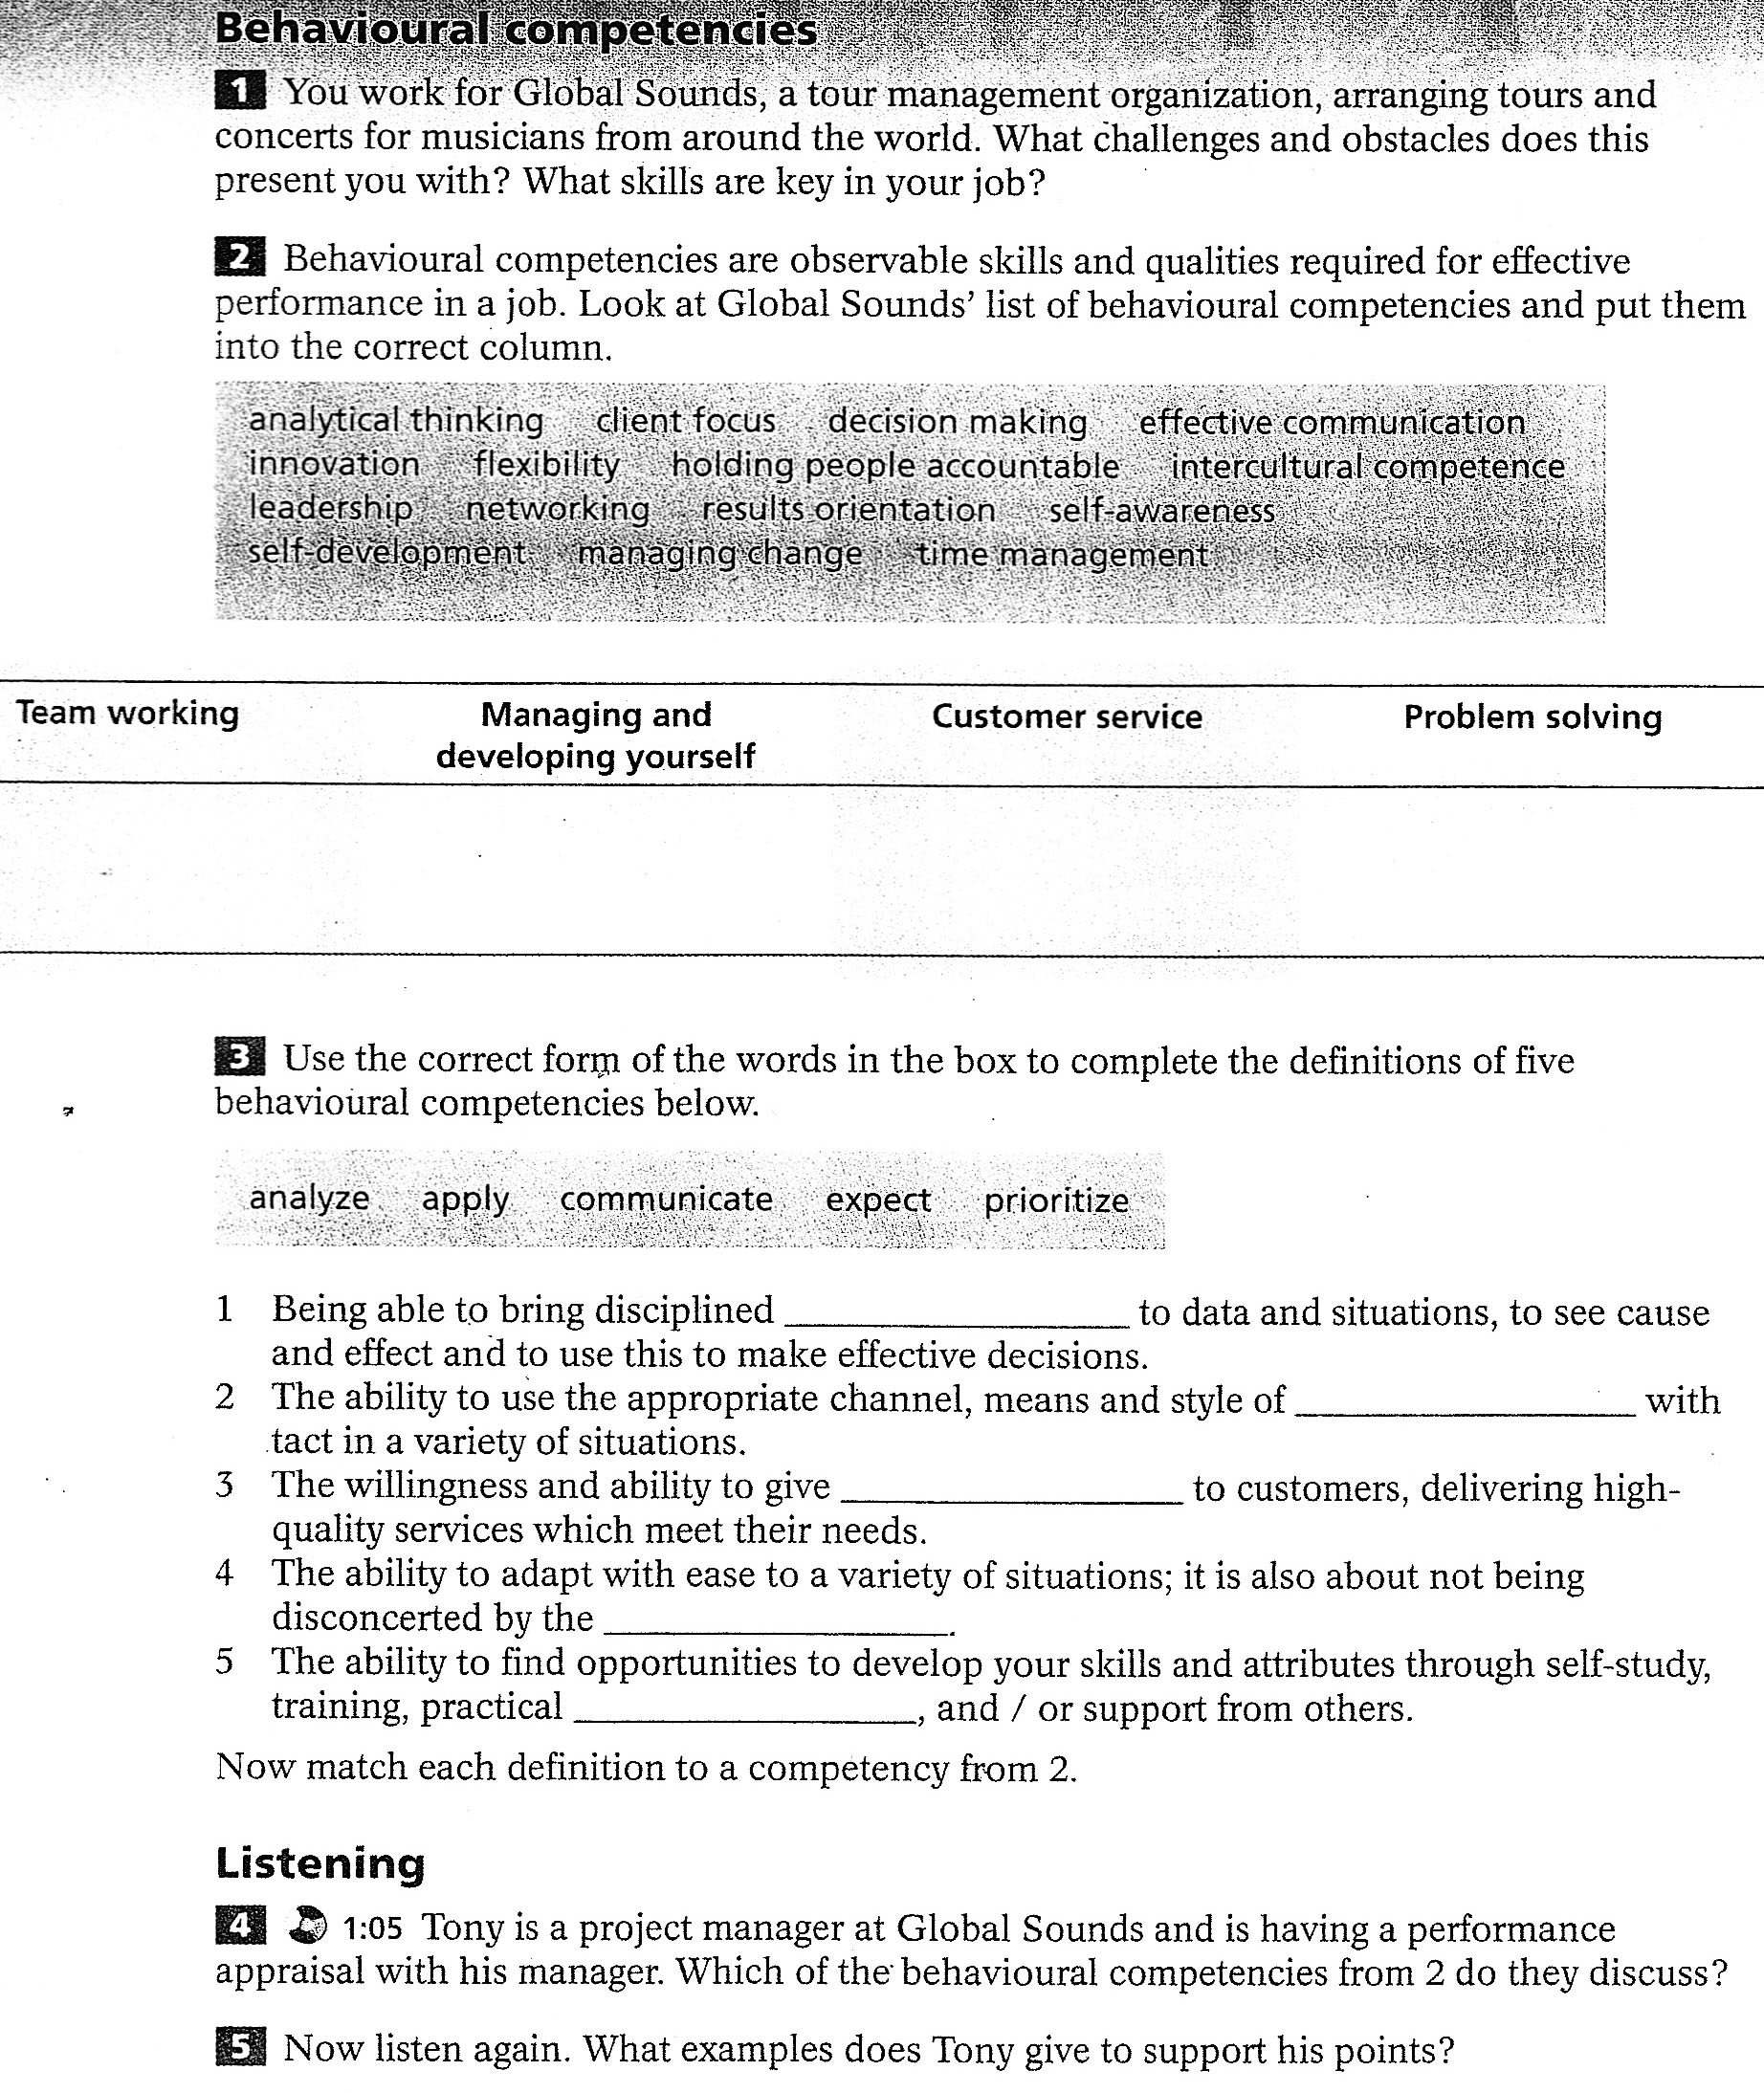
\includegraphics[scale=.85]{handouts/Eng303.jpg}
\section{Management Skills}
%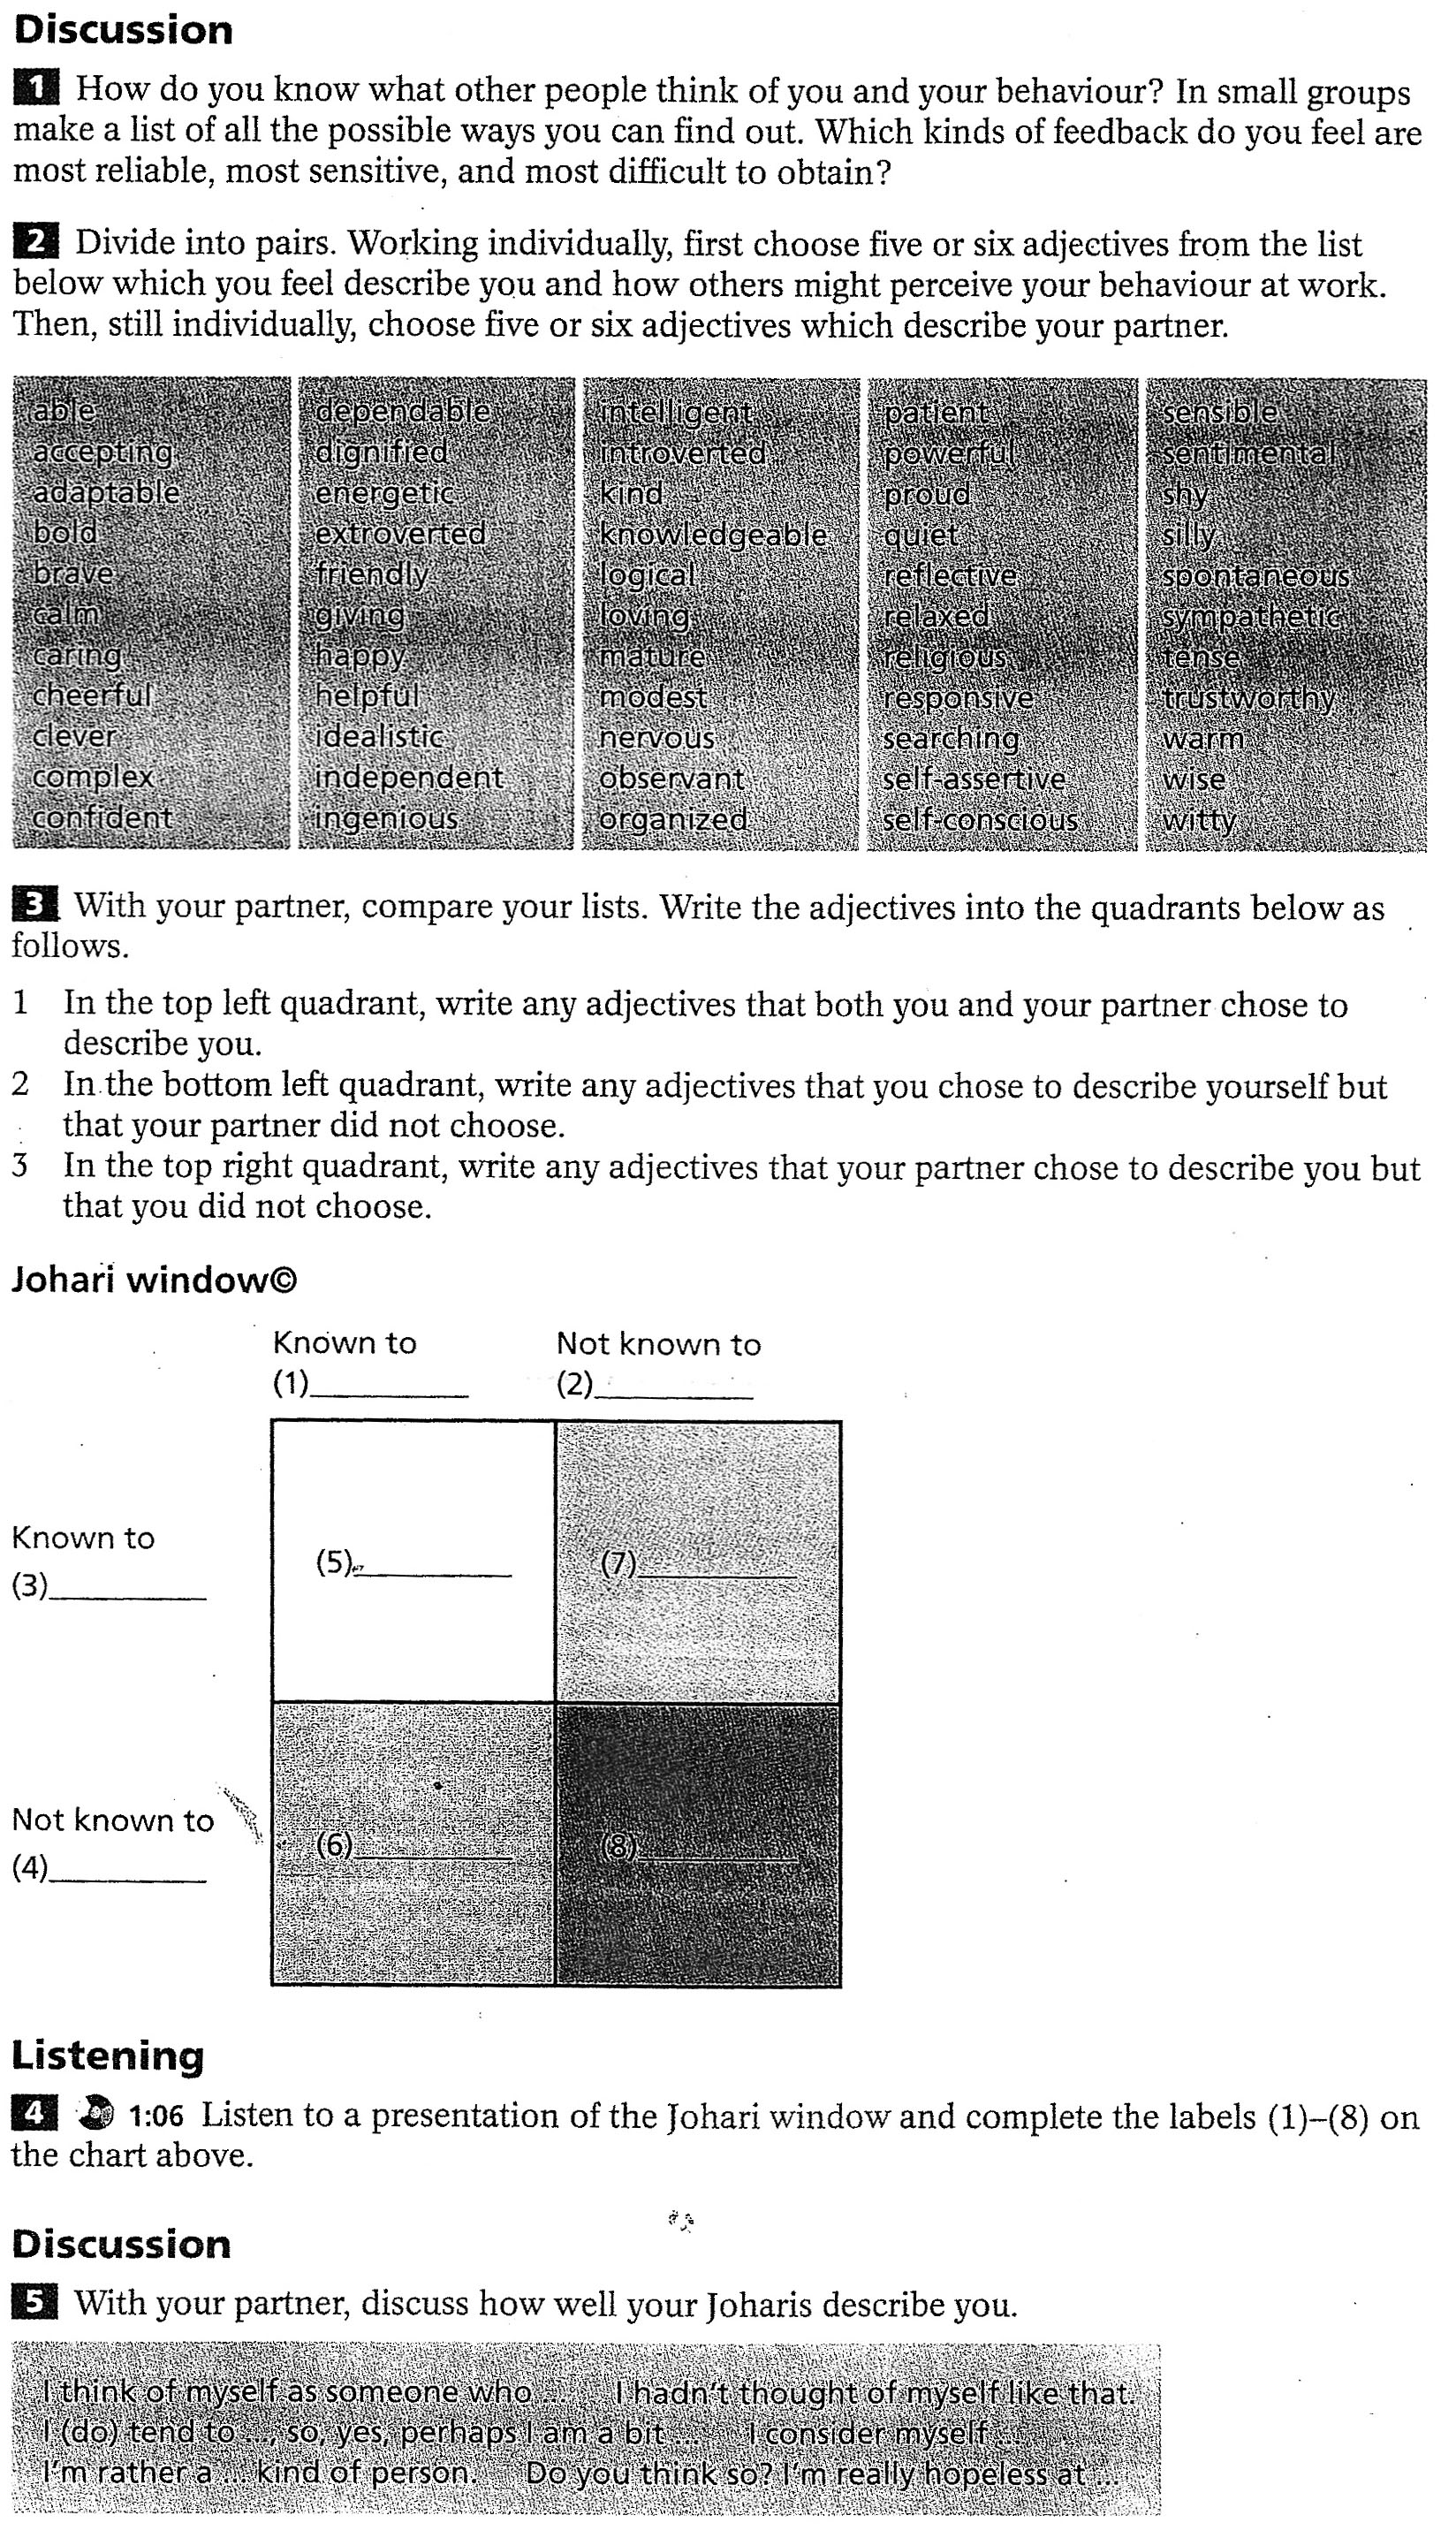
\includegraphics[scale=.85]{handouts/Eng305.jpg}

%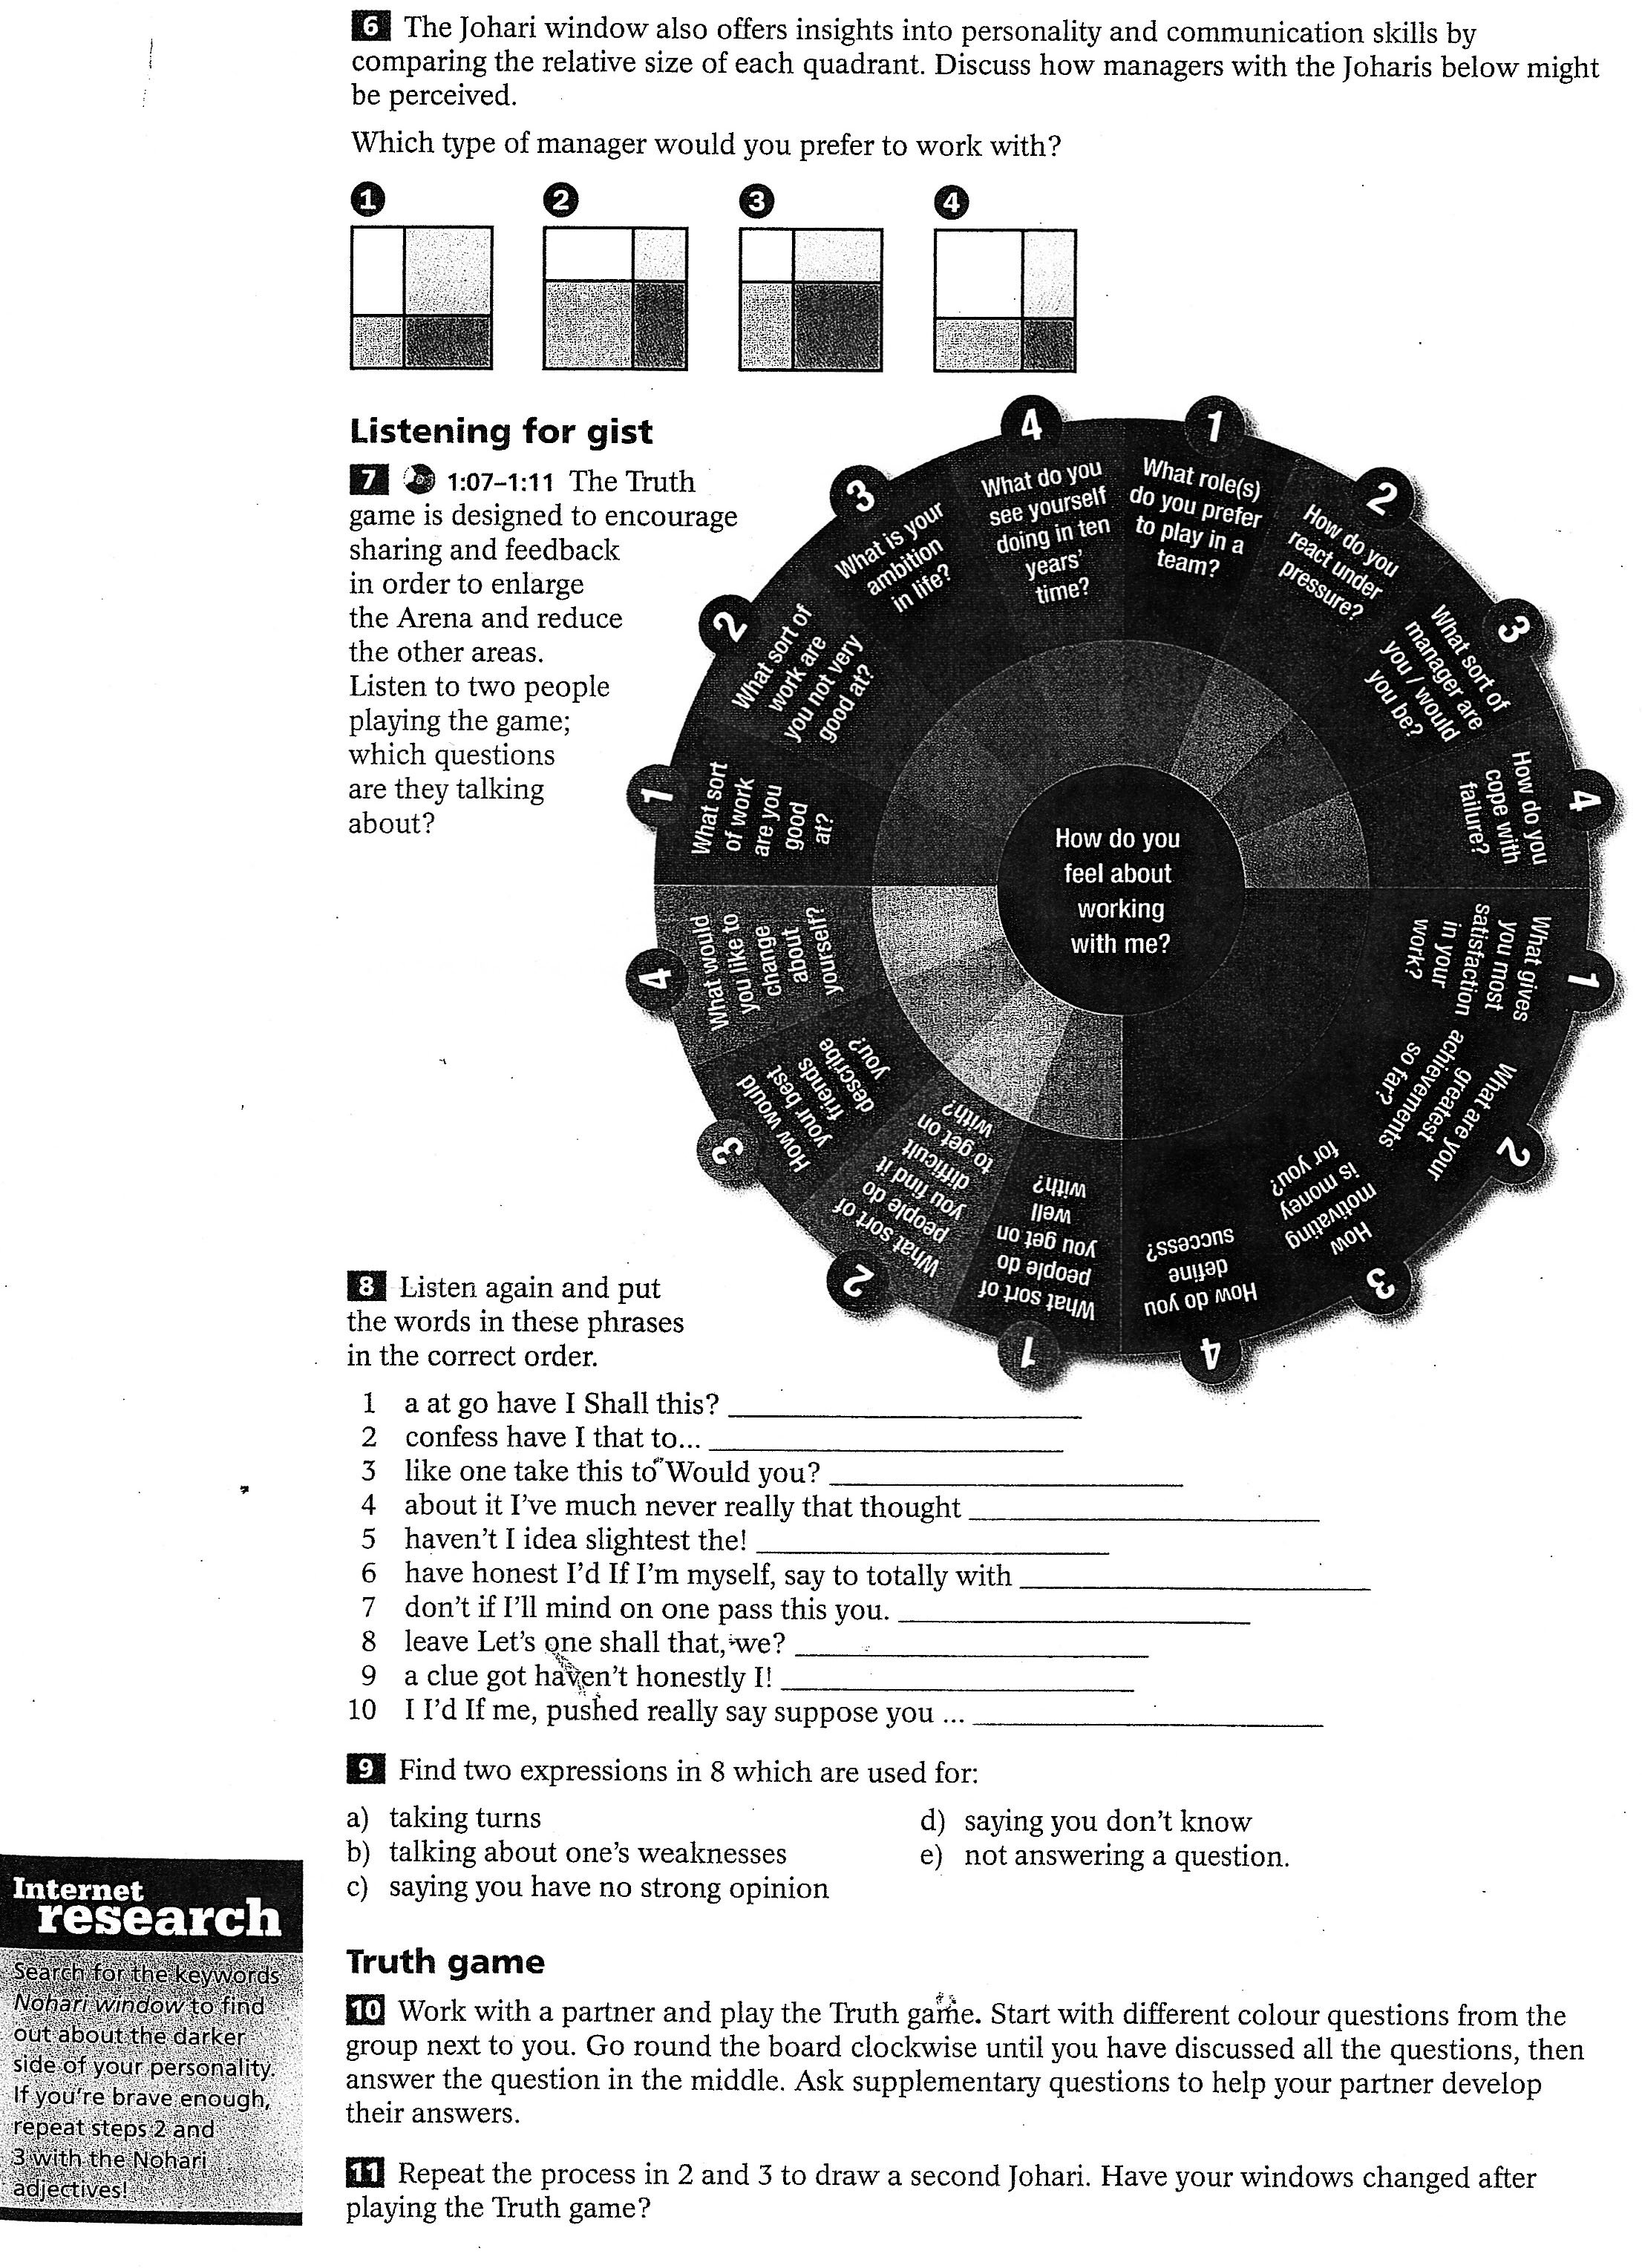
\includegraphics[scale=.85]{handouts/Eng306.jpg}
\section{Writing}
%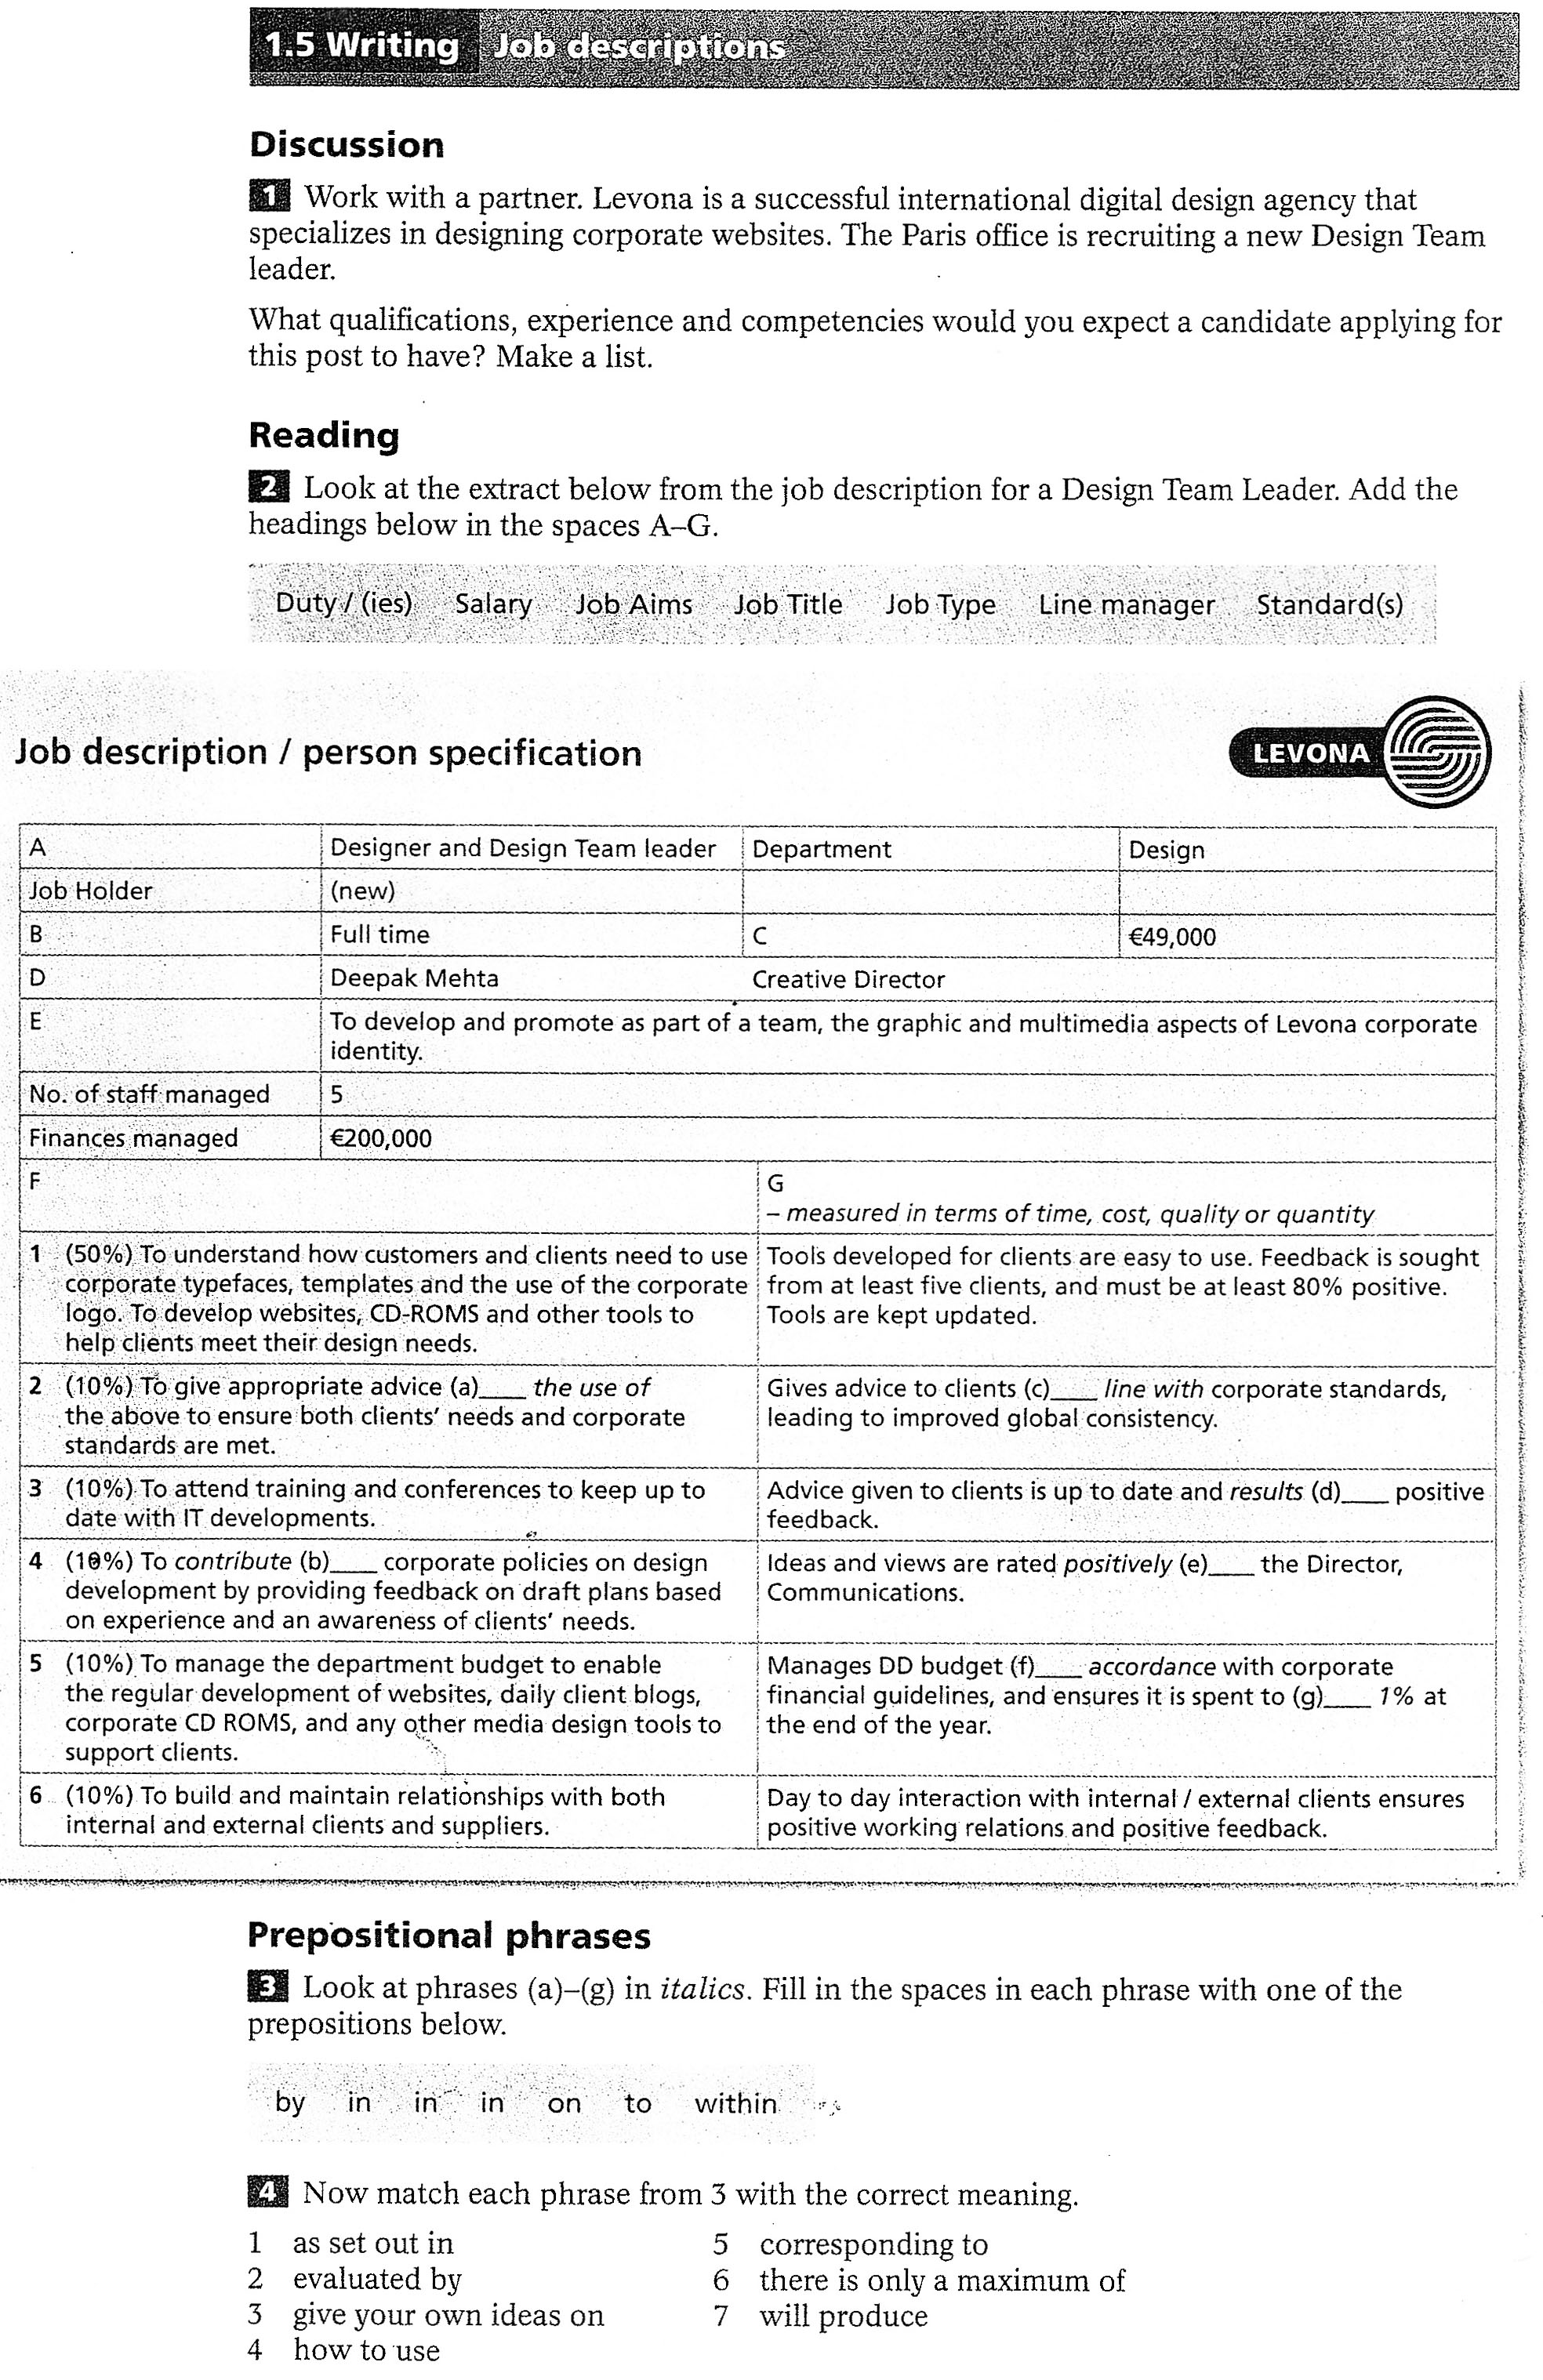
\includegraphics[scale=.85]{handouts/Eng307.jpg}

%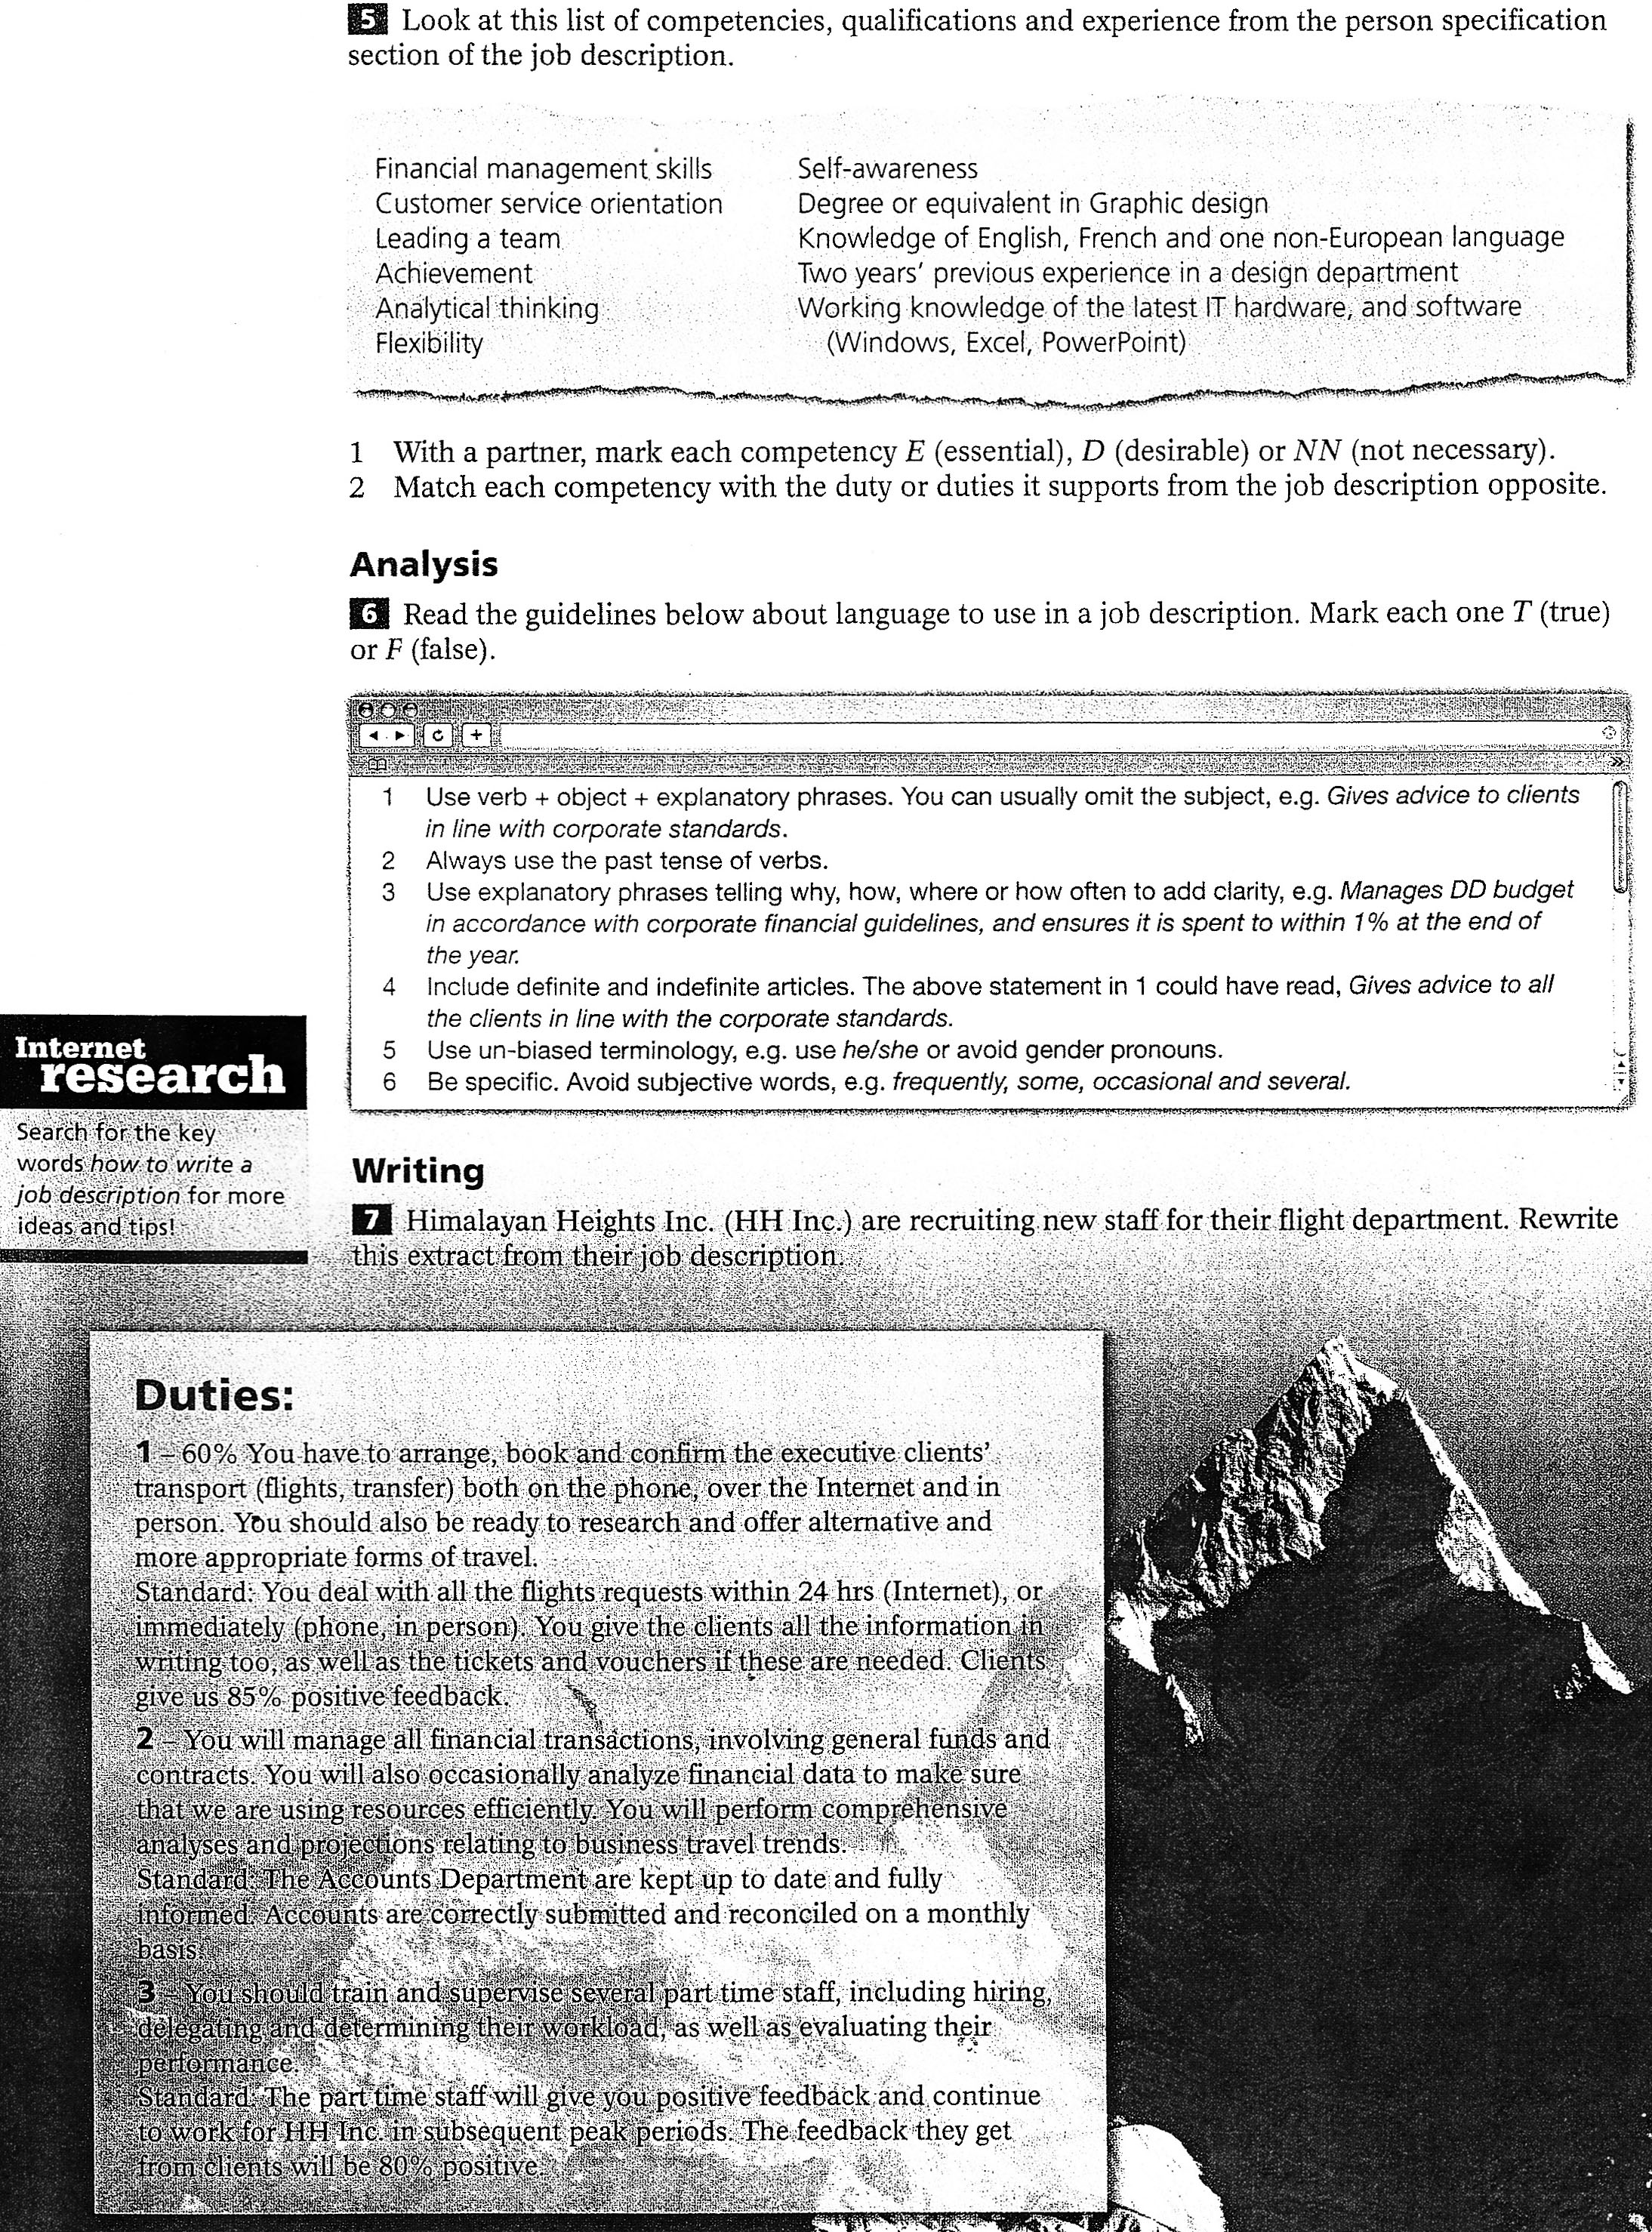
\includegraphics[scale=.85]{handouts/Eng308.jpg}
\section{Gerund and infinitive}
%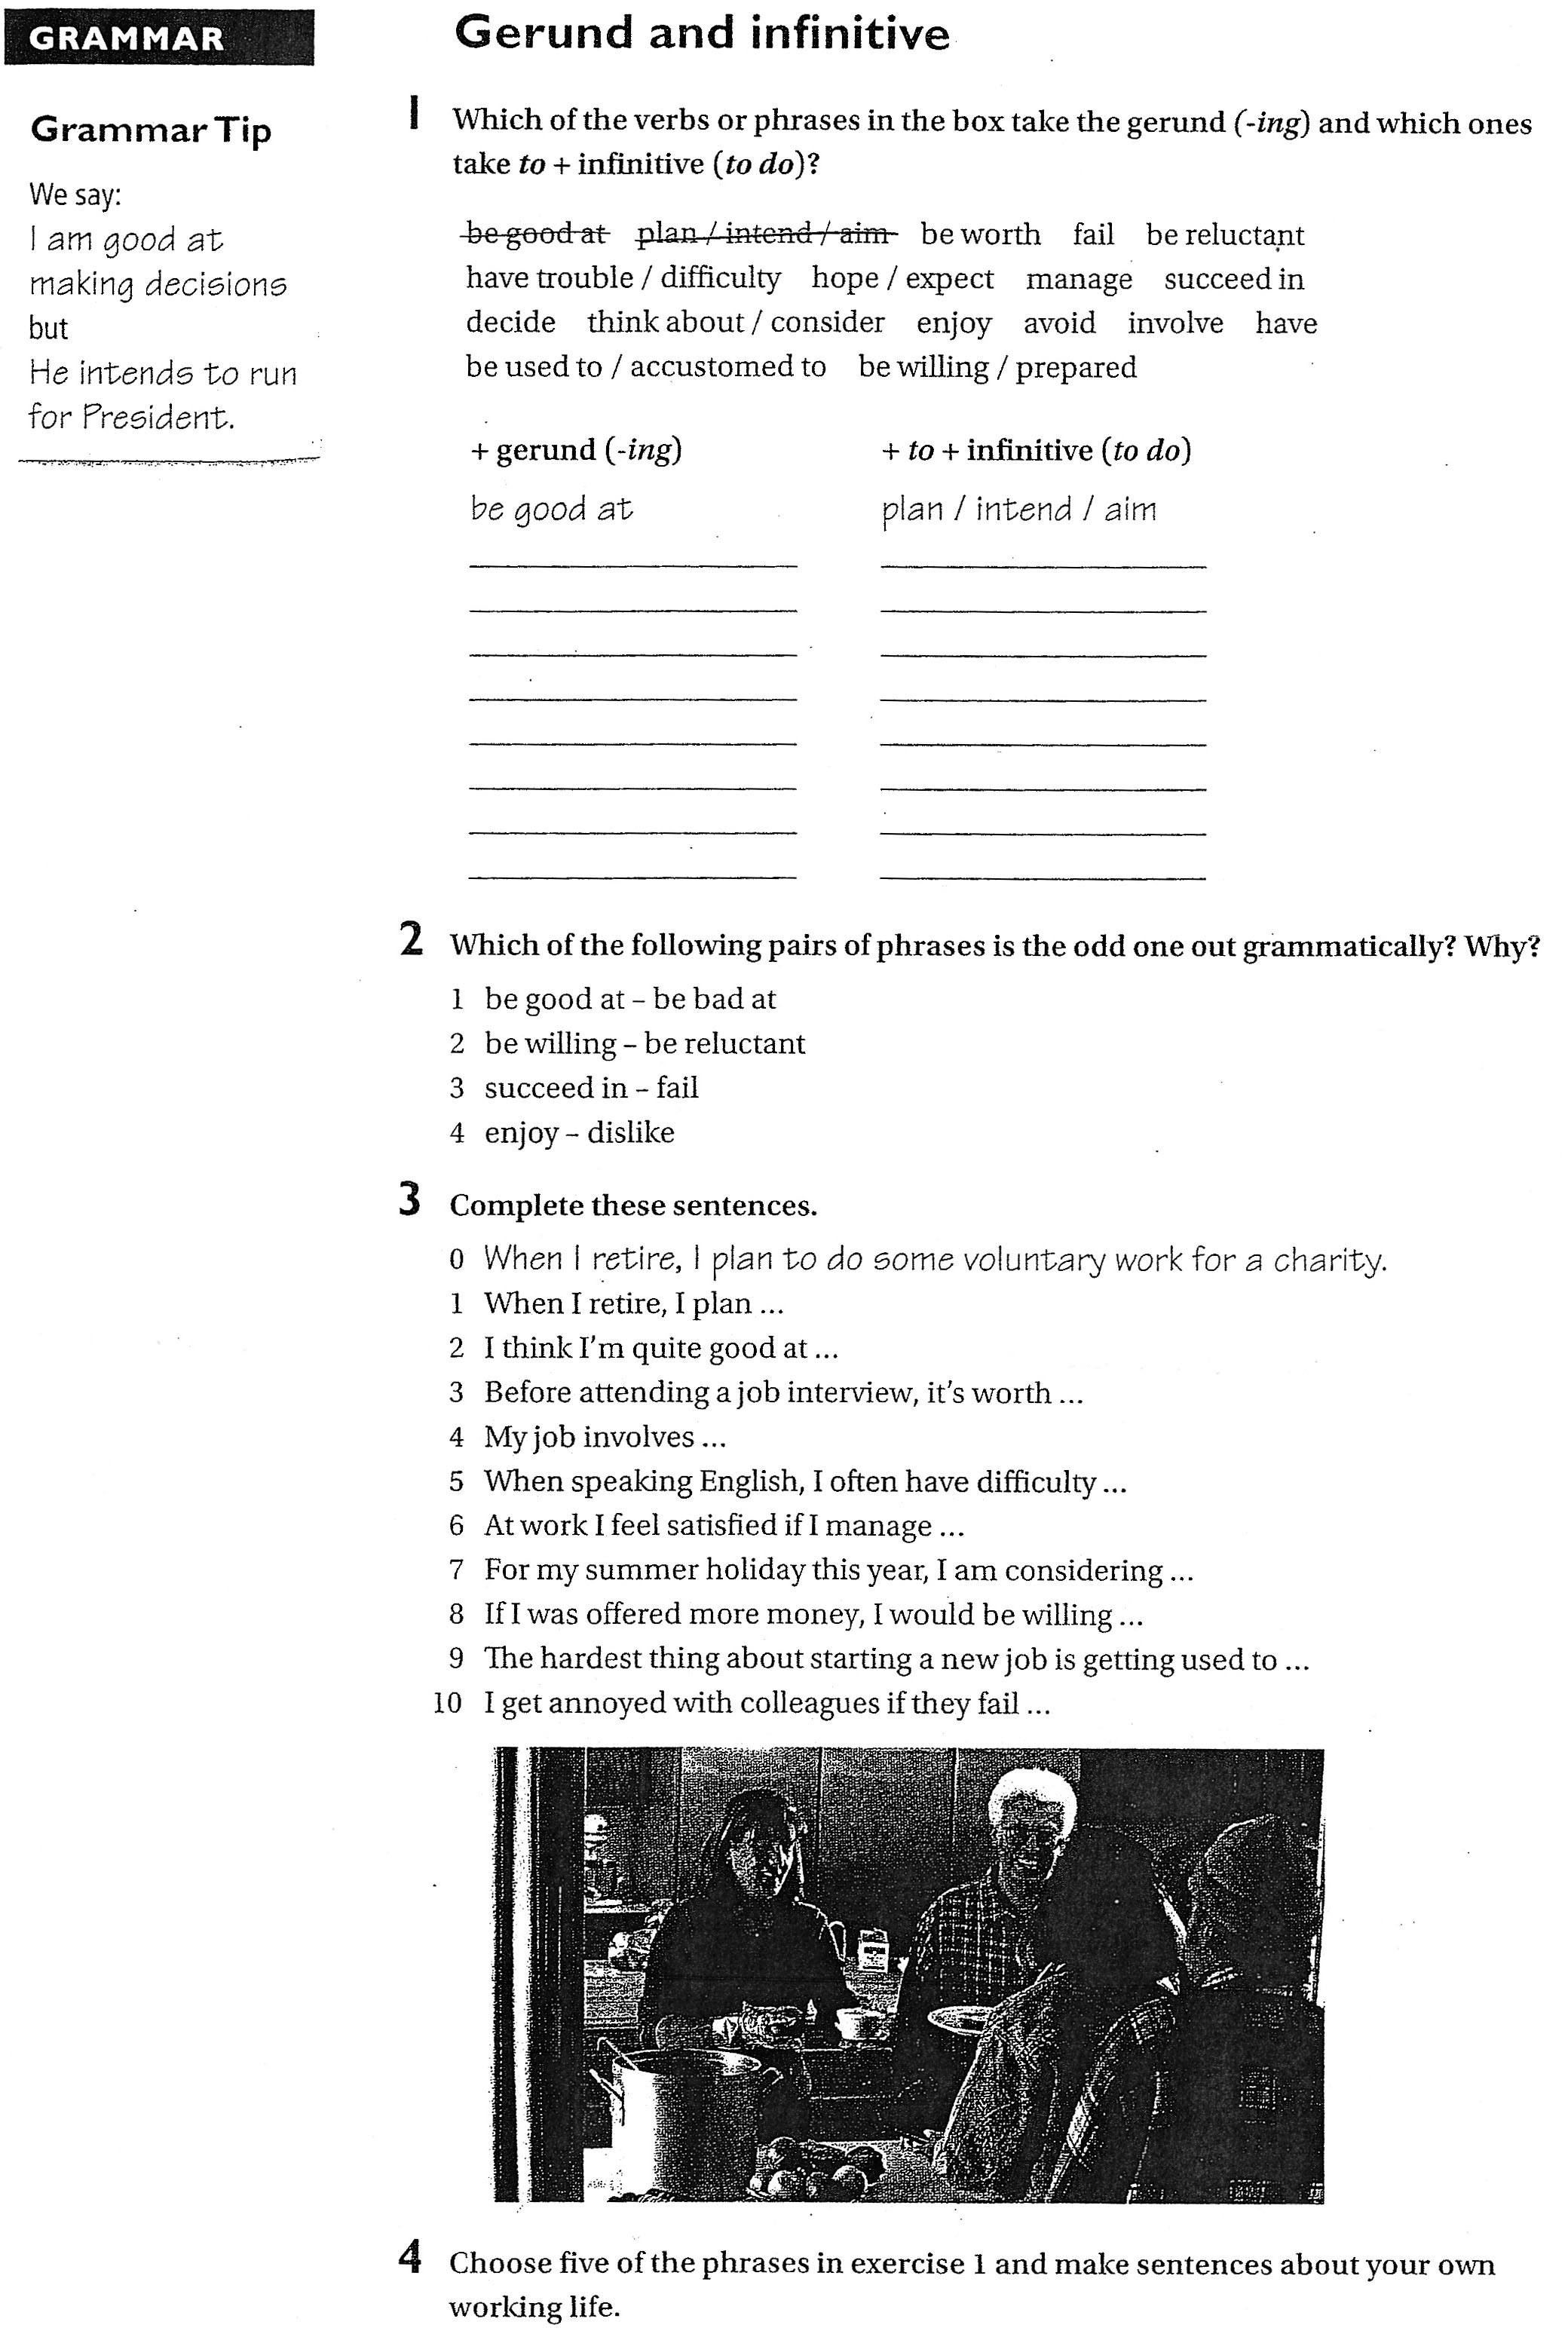
\includegraphics[scale=.85]{handouts/Eng309.jpg}
\section{Job Applications for Mechanical Engineering Students}
%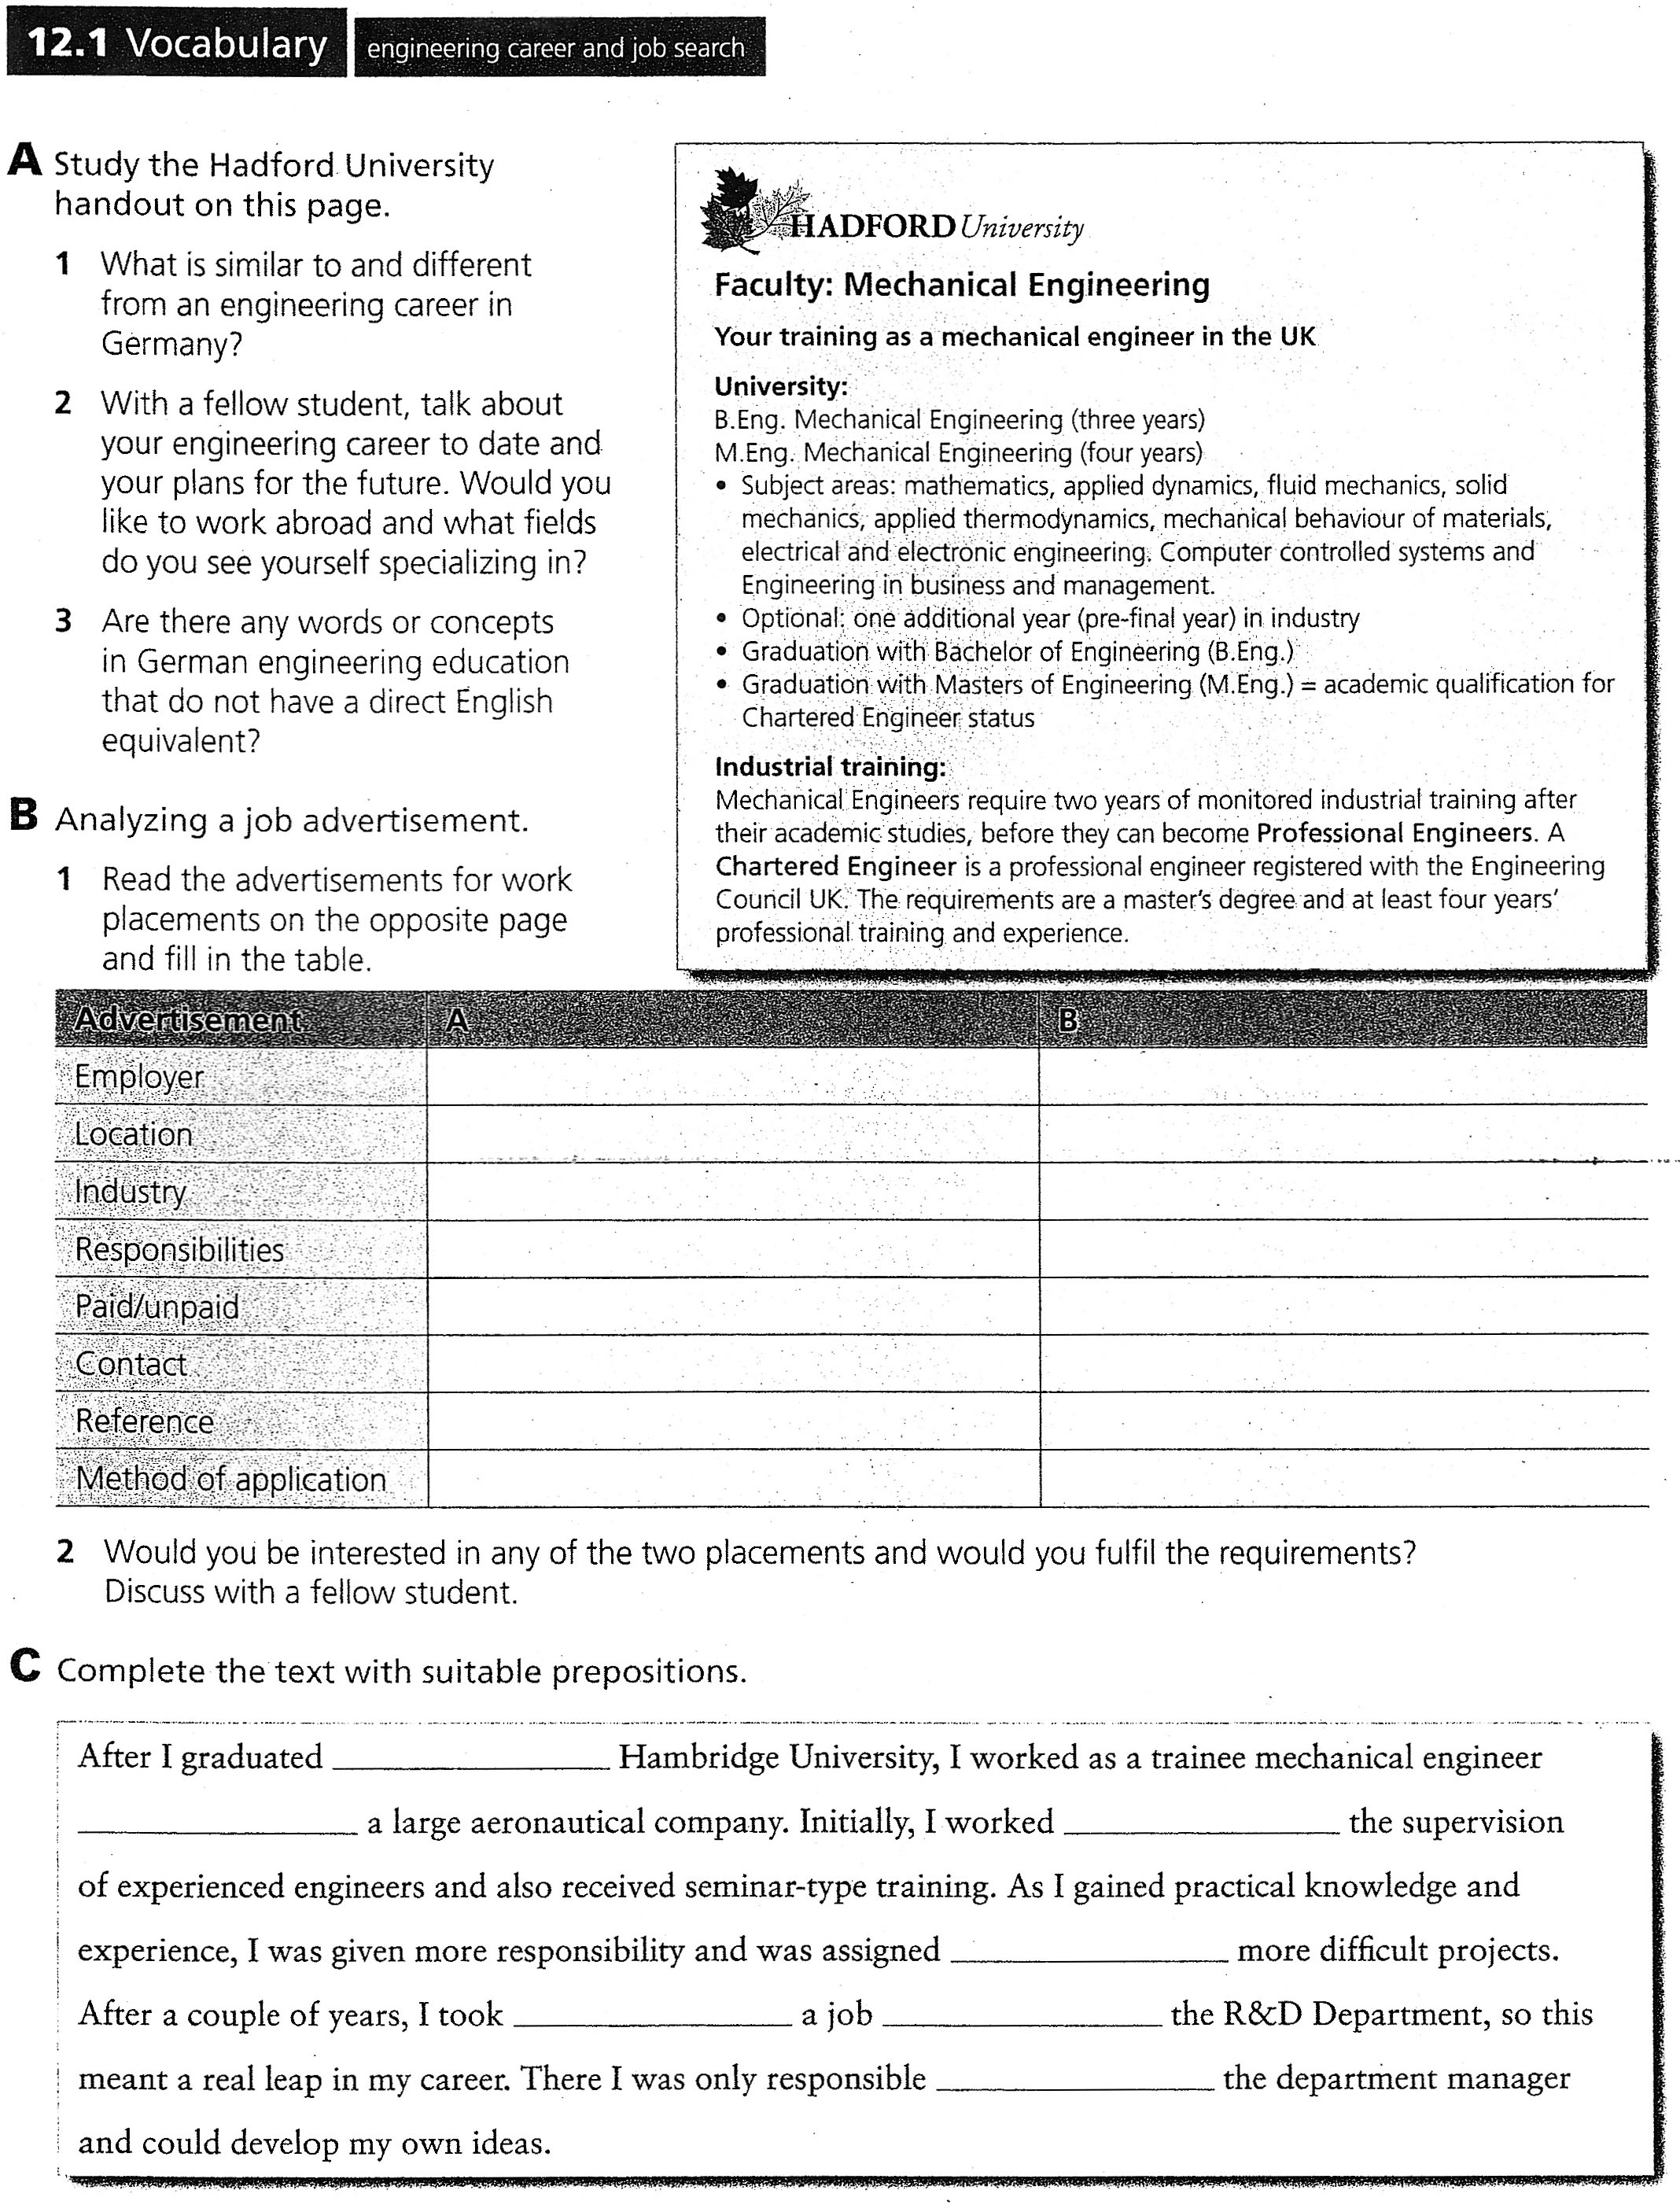
\includegraphics[scale=.85]{handouts/Eng311.jpg}

%
\includegraphics[scale=.85]{handouts/Eng312.jpg}


\chapter{Applying for an Internship}
Career Express B2: Unit 1 Applying for an Internship

%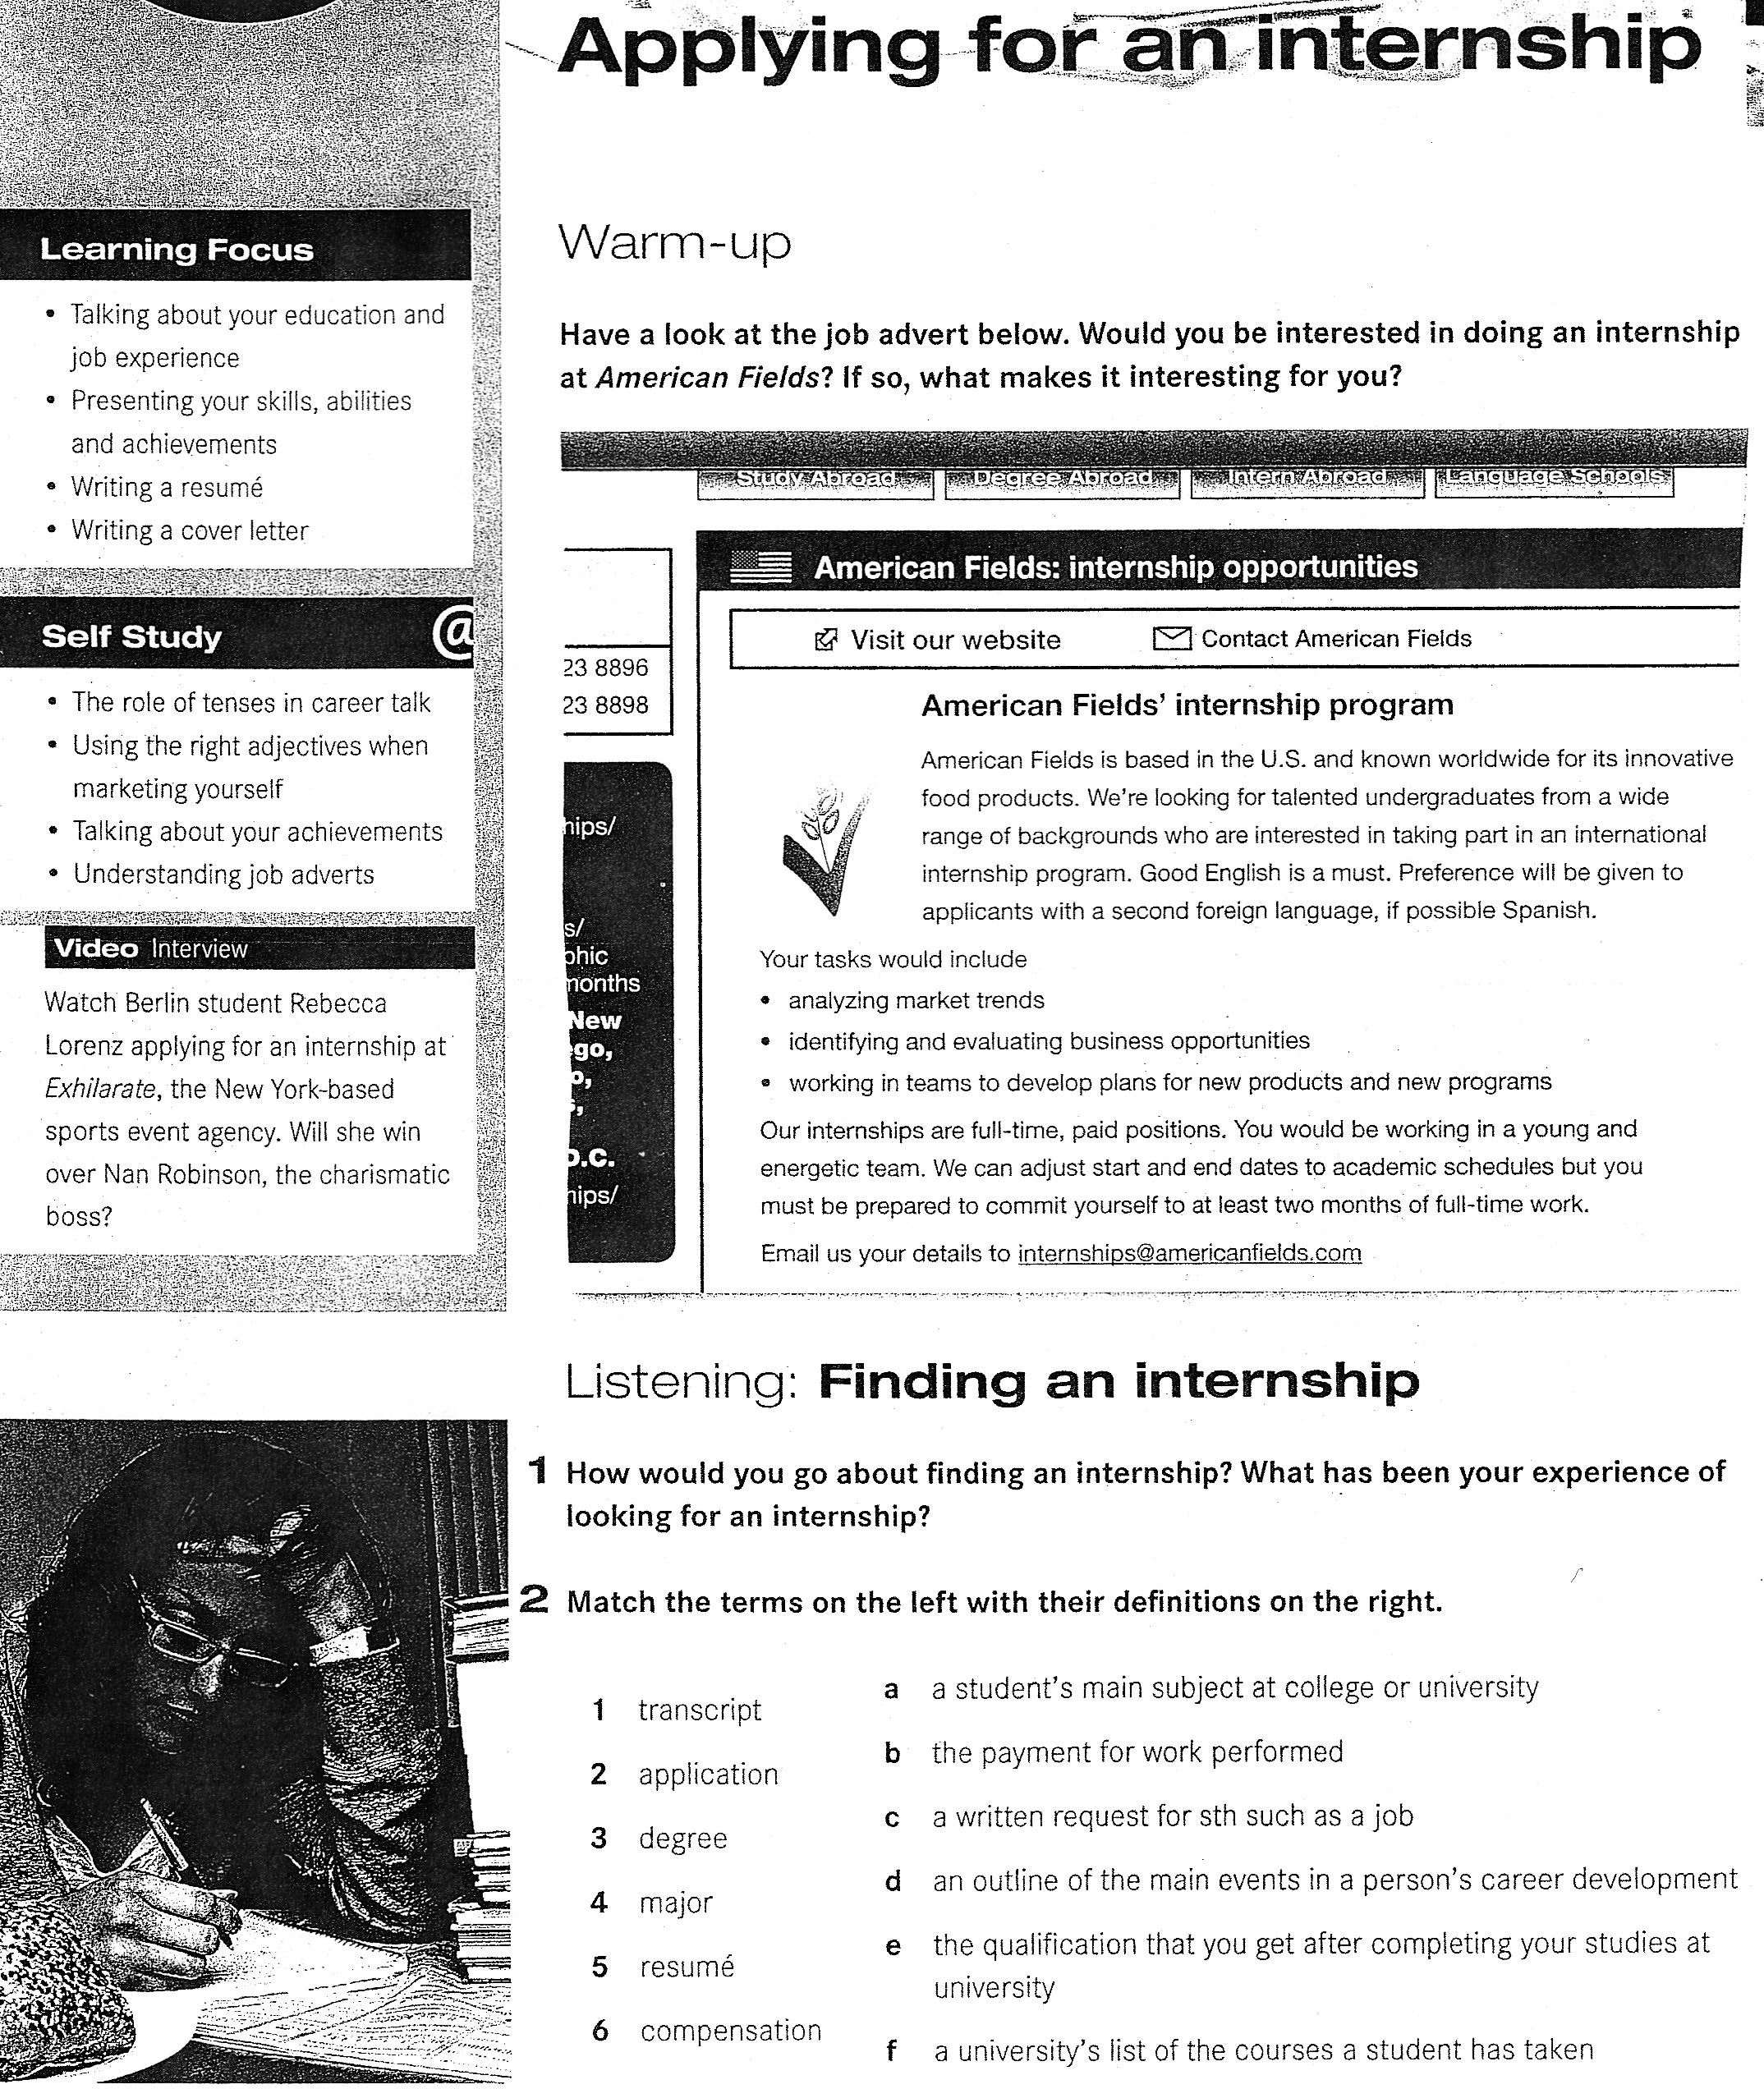
\includegraphics[scale=.85]{handouts/Eng401.jpg}

%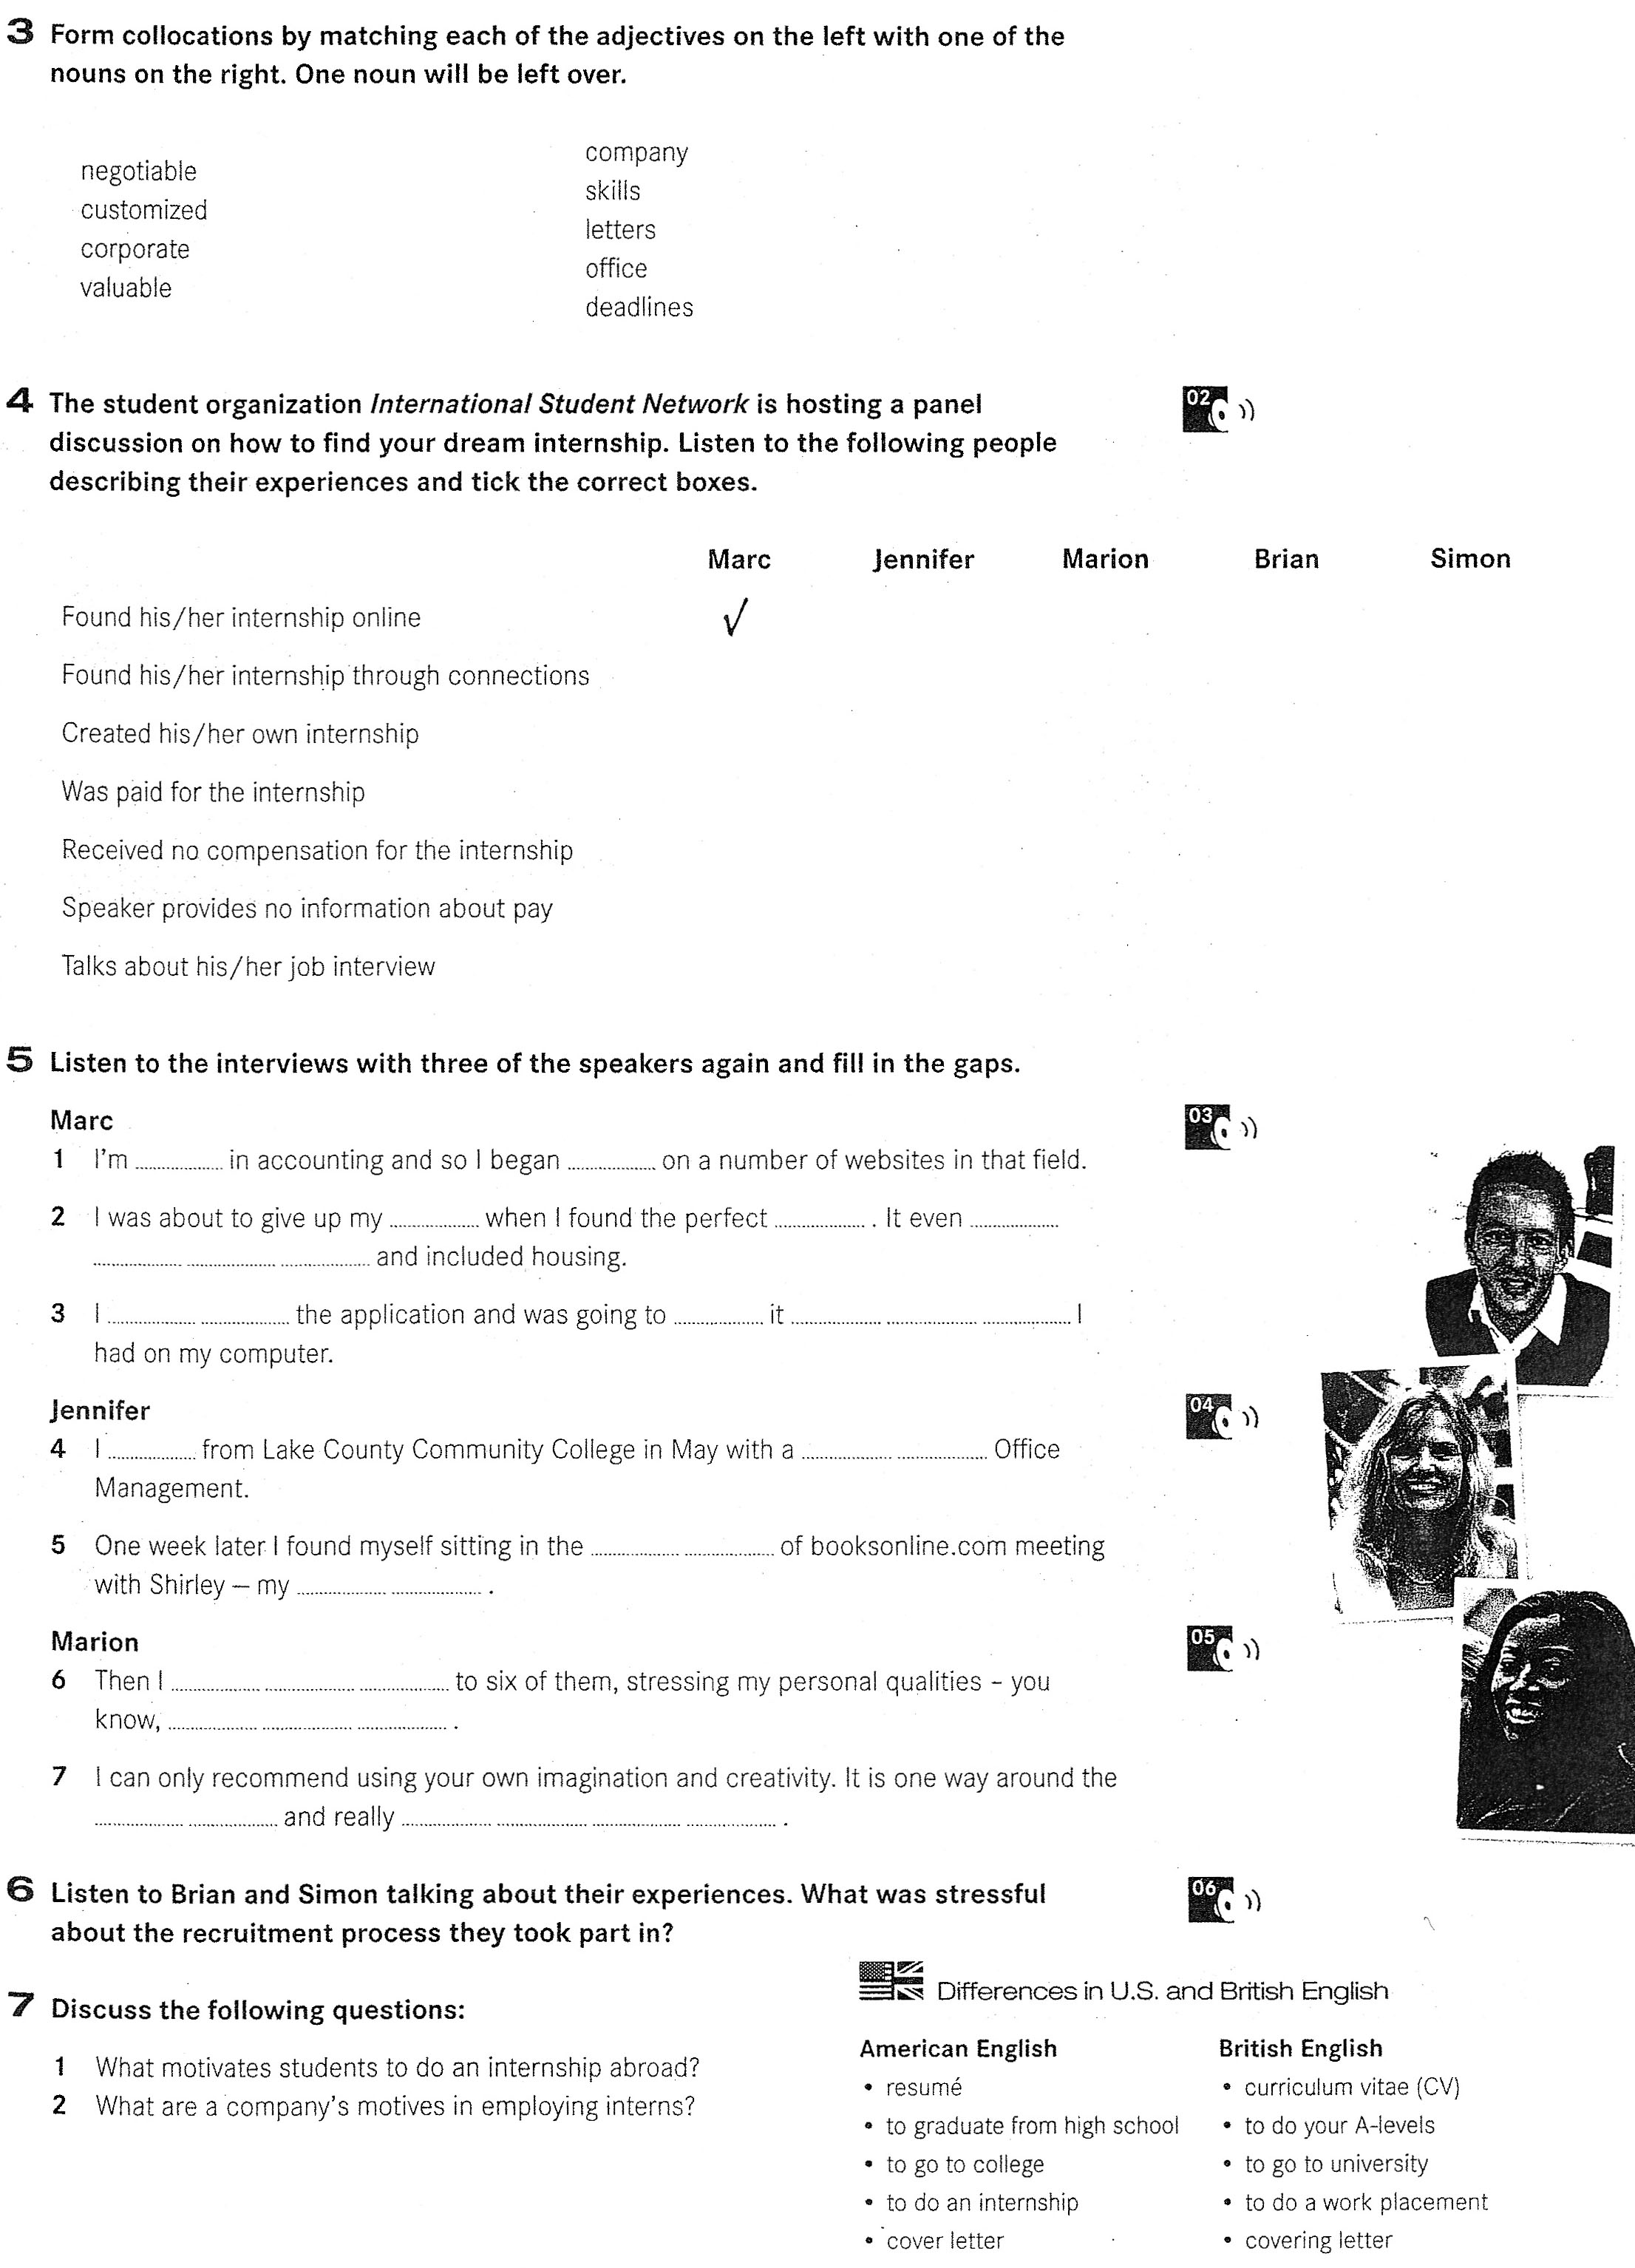
\includegraphics[scale=.85]{handouts/Eng402.jpg}

%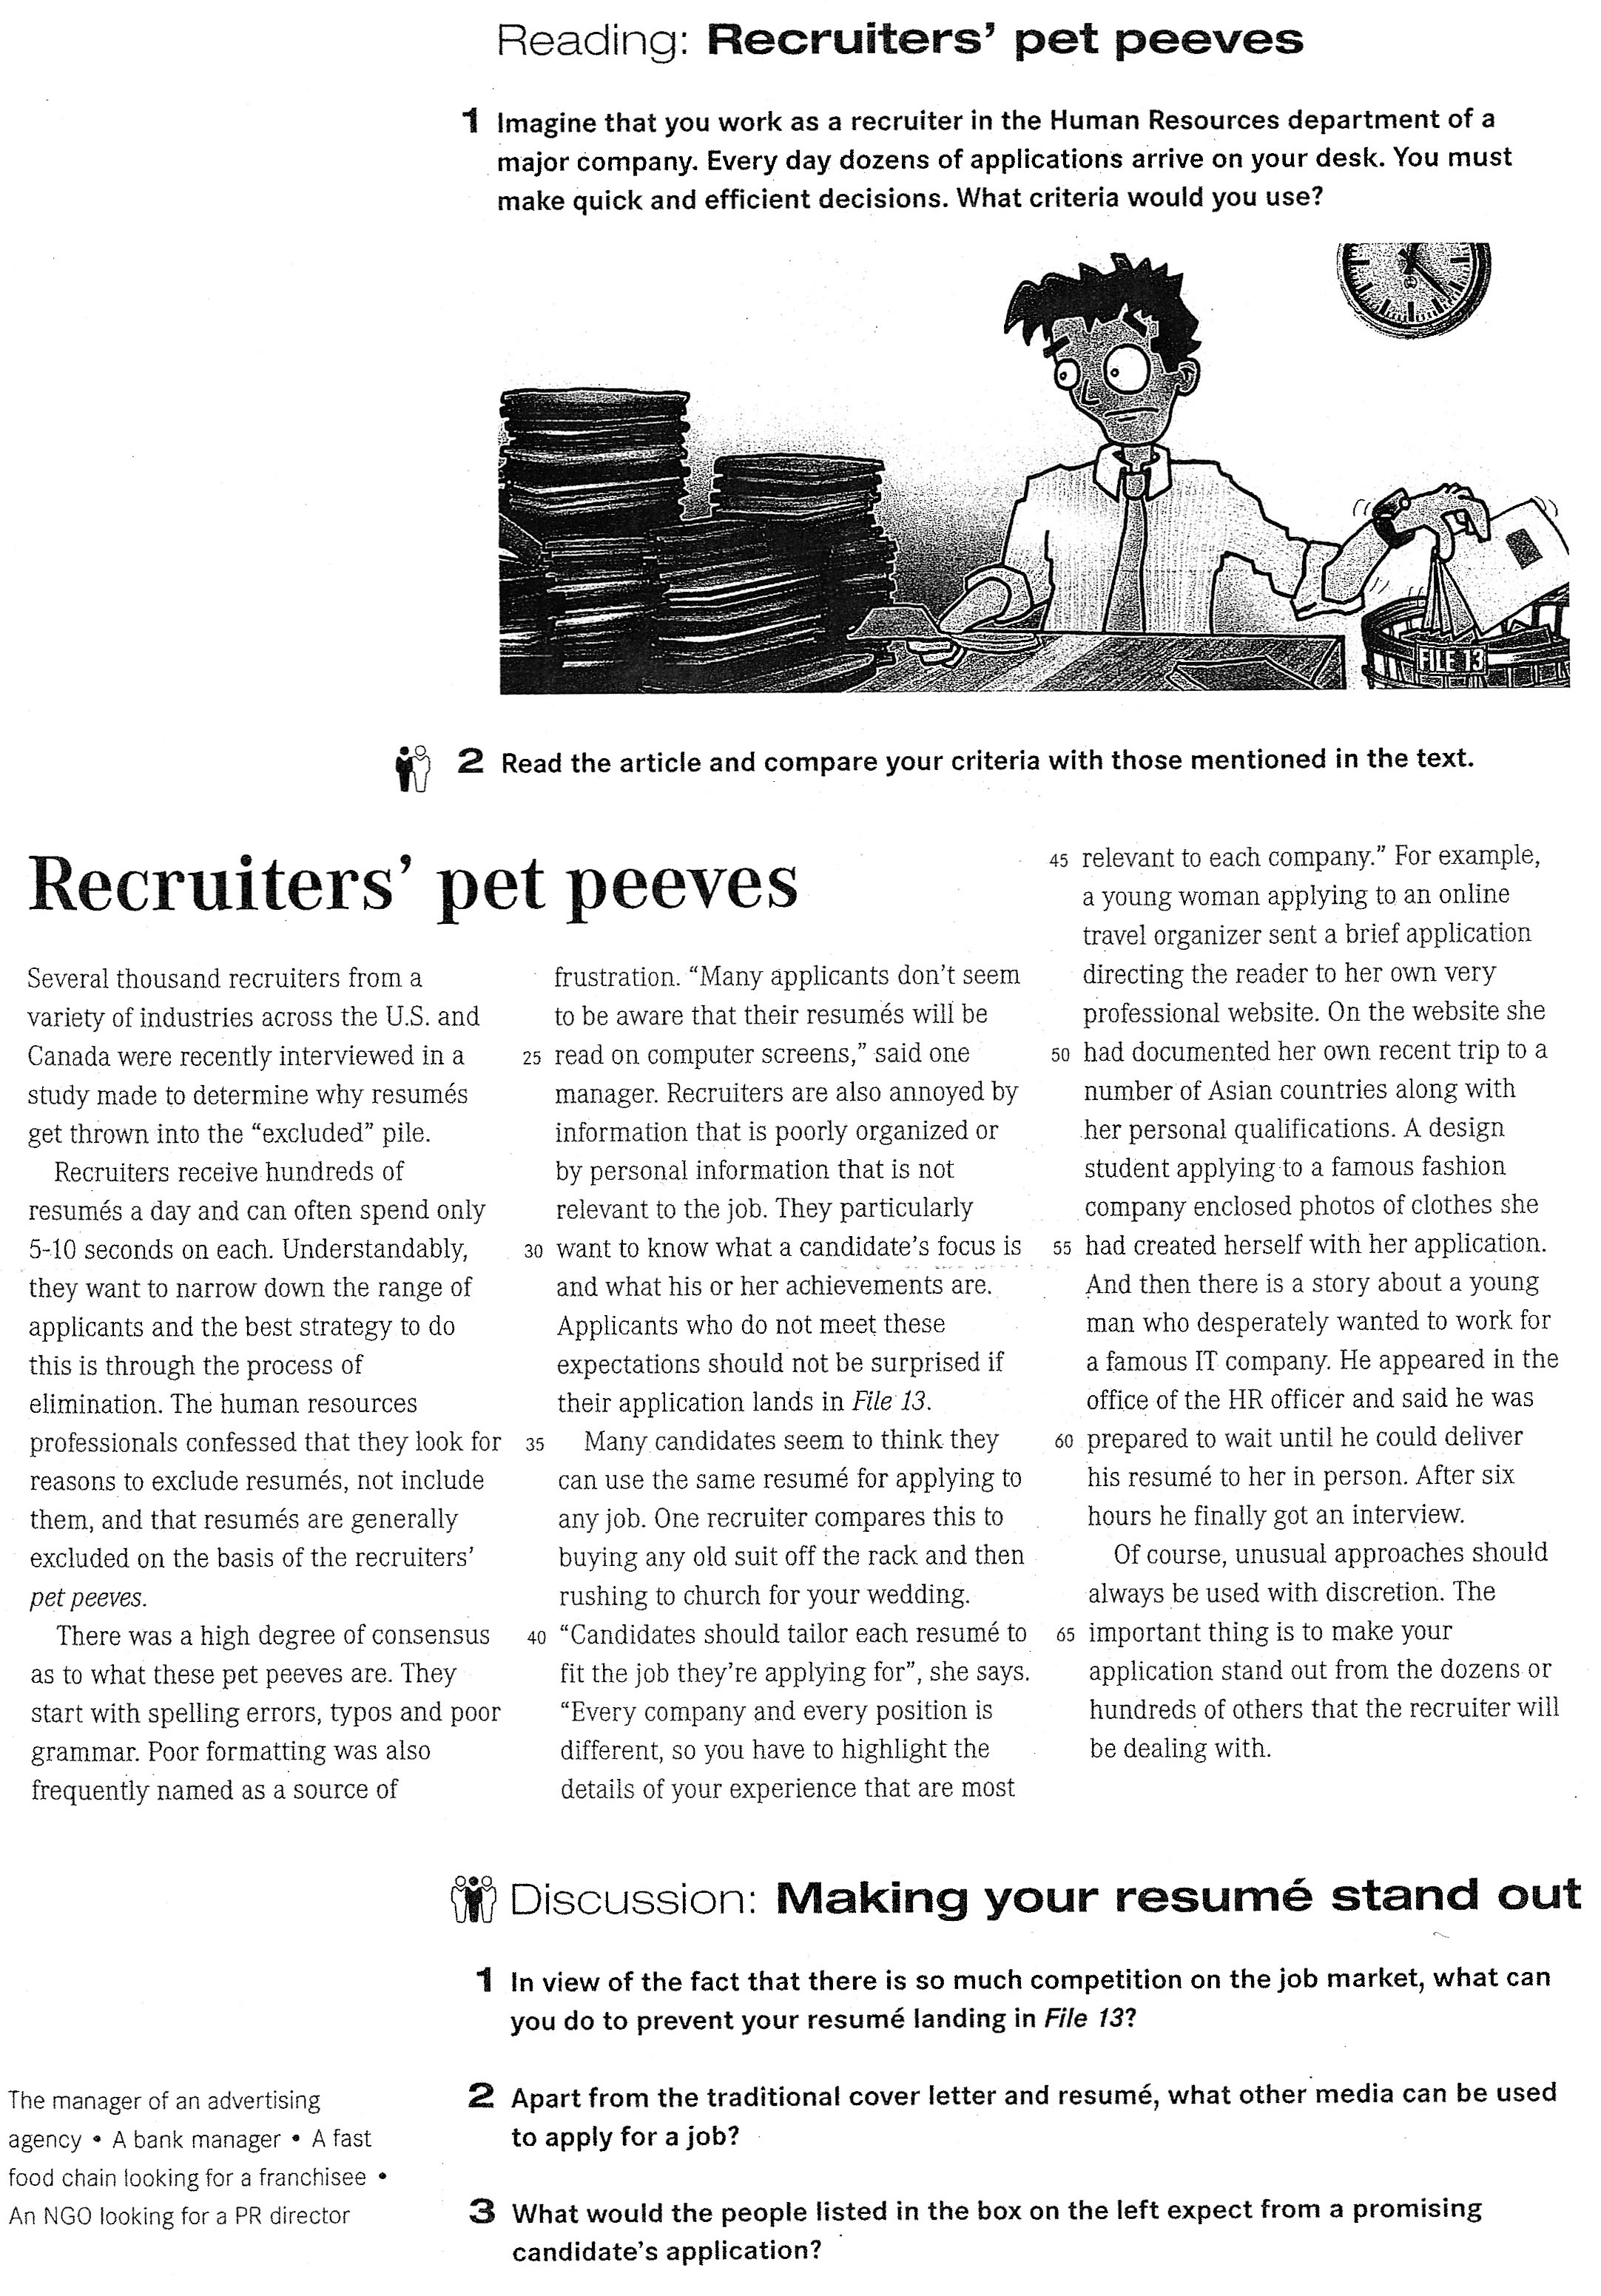
\includegraphics[scale=.85]{handouts/Eng403.jpg}

%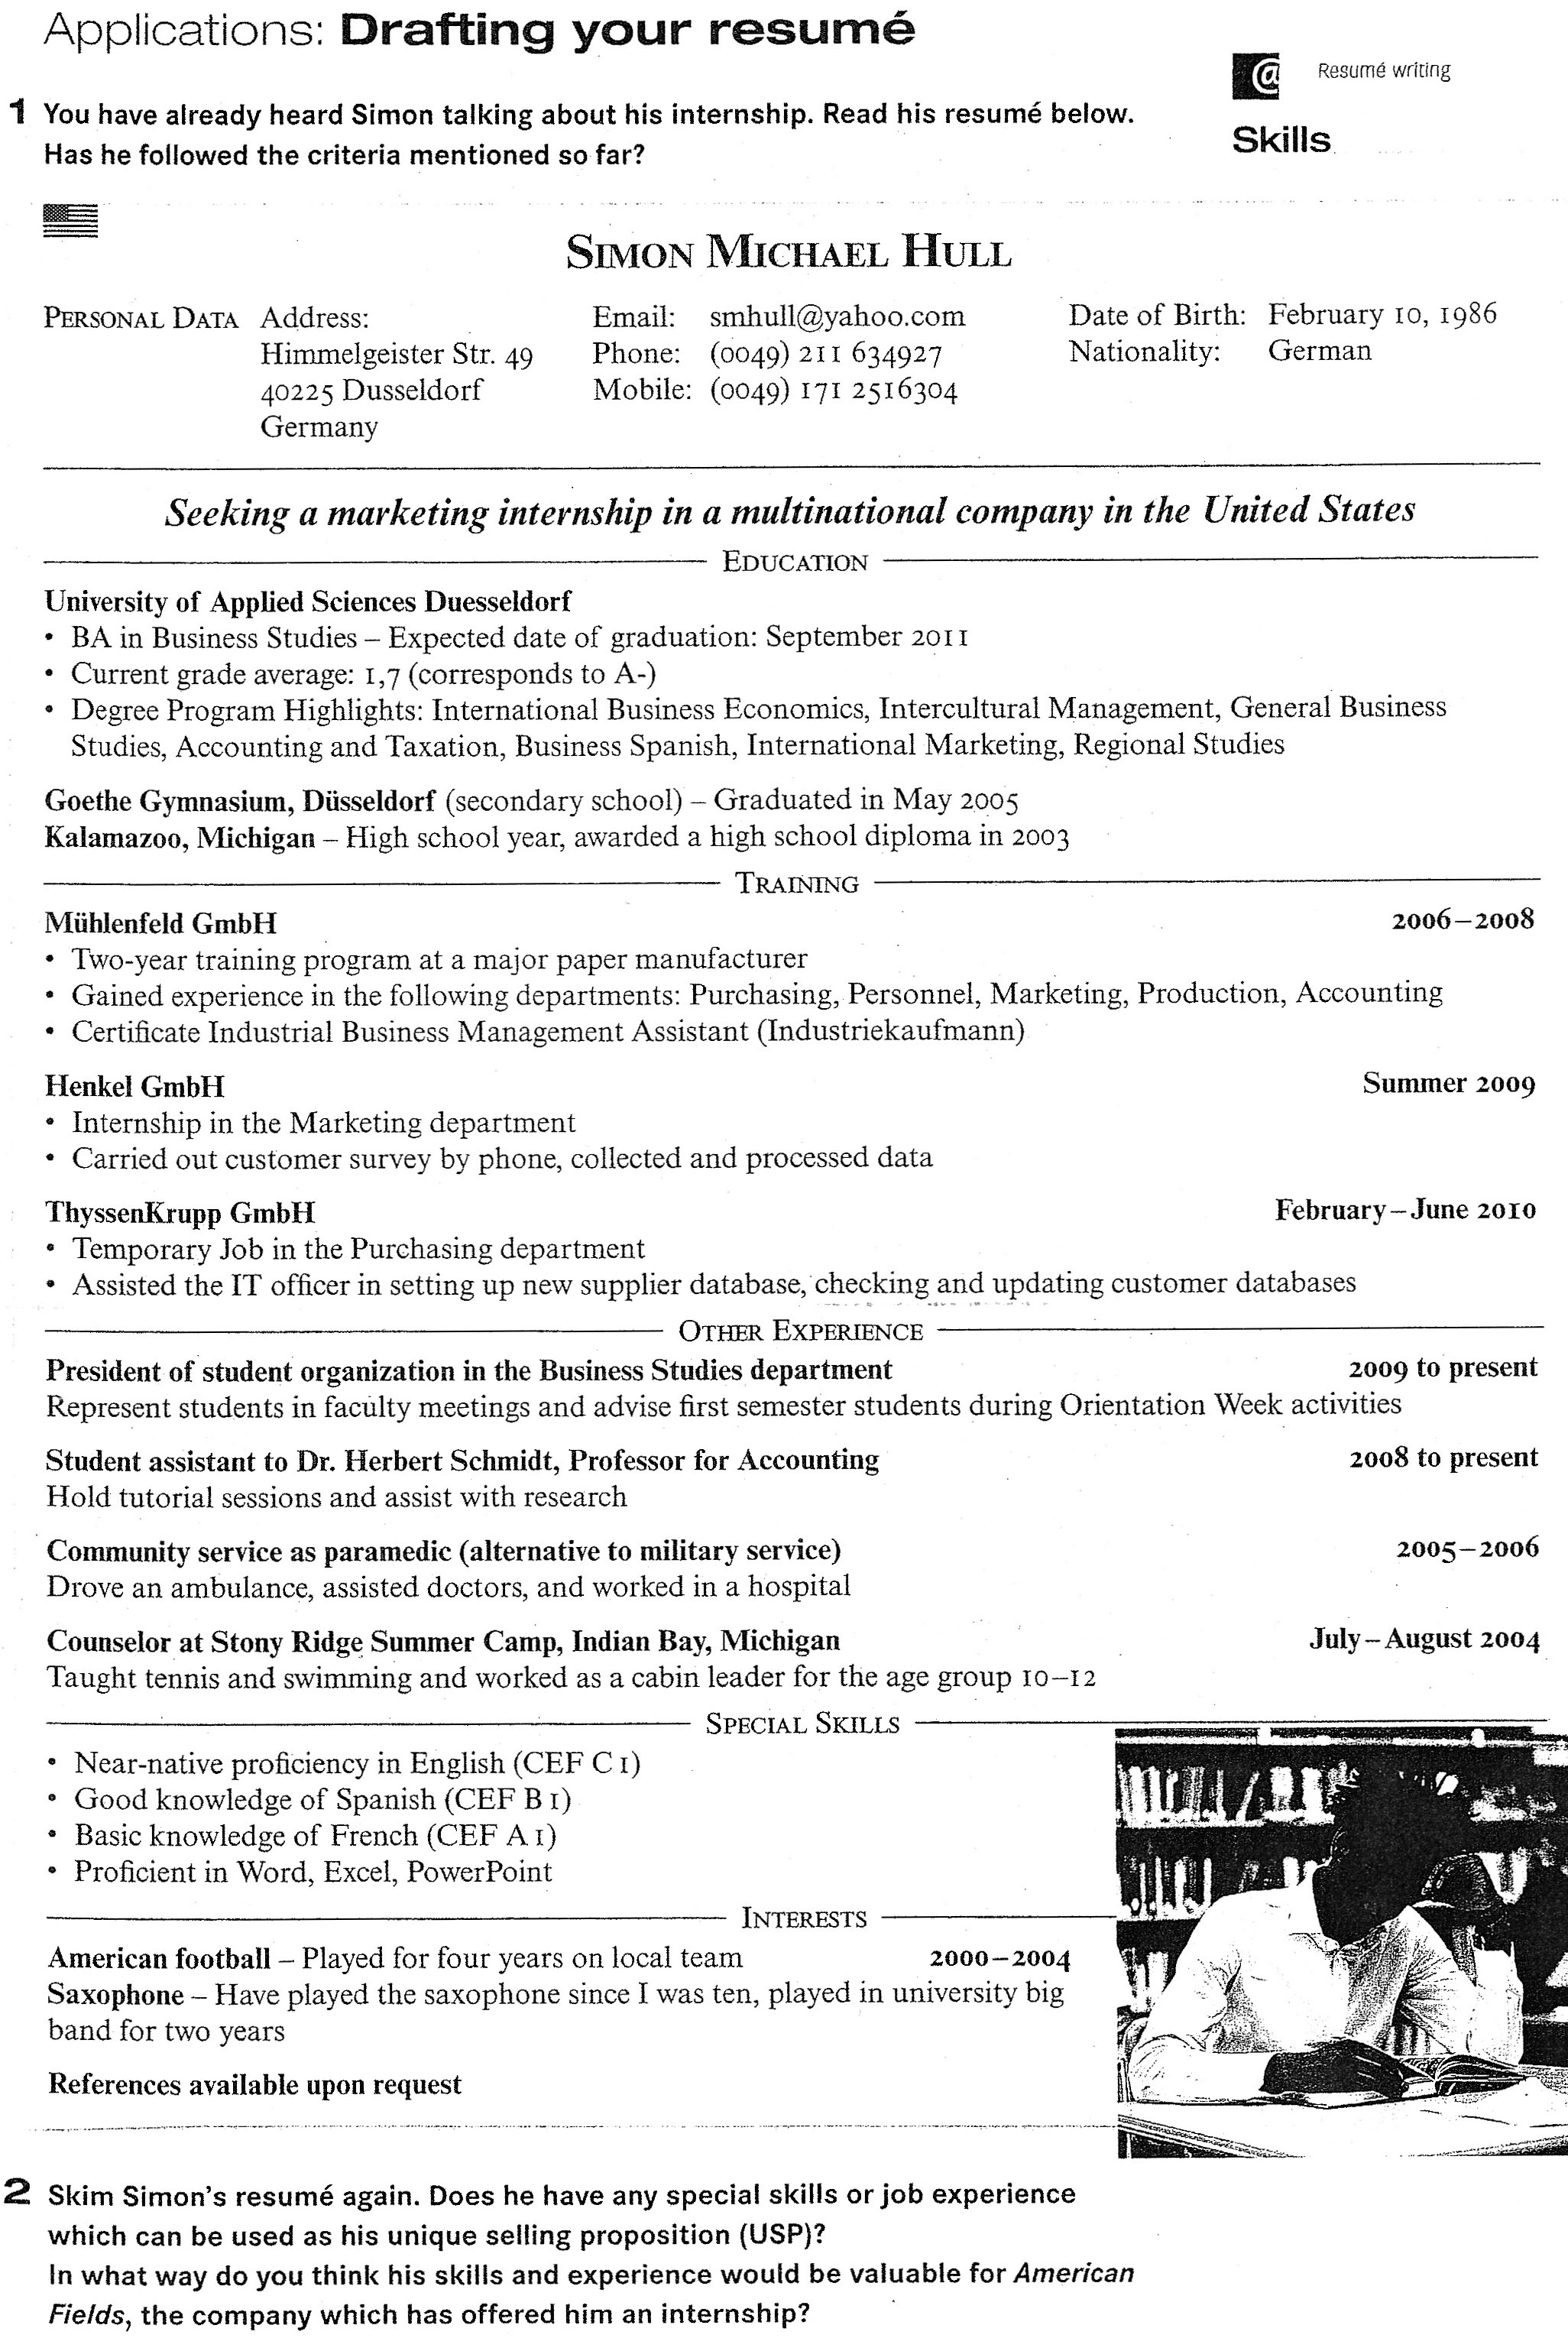
\includegraphics[scale=.85]{handouts/Eng404.jpg}

%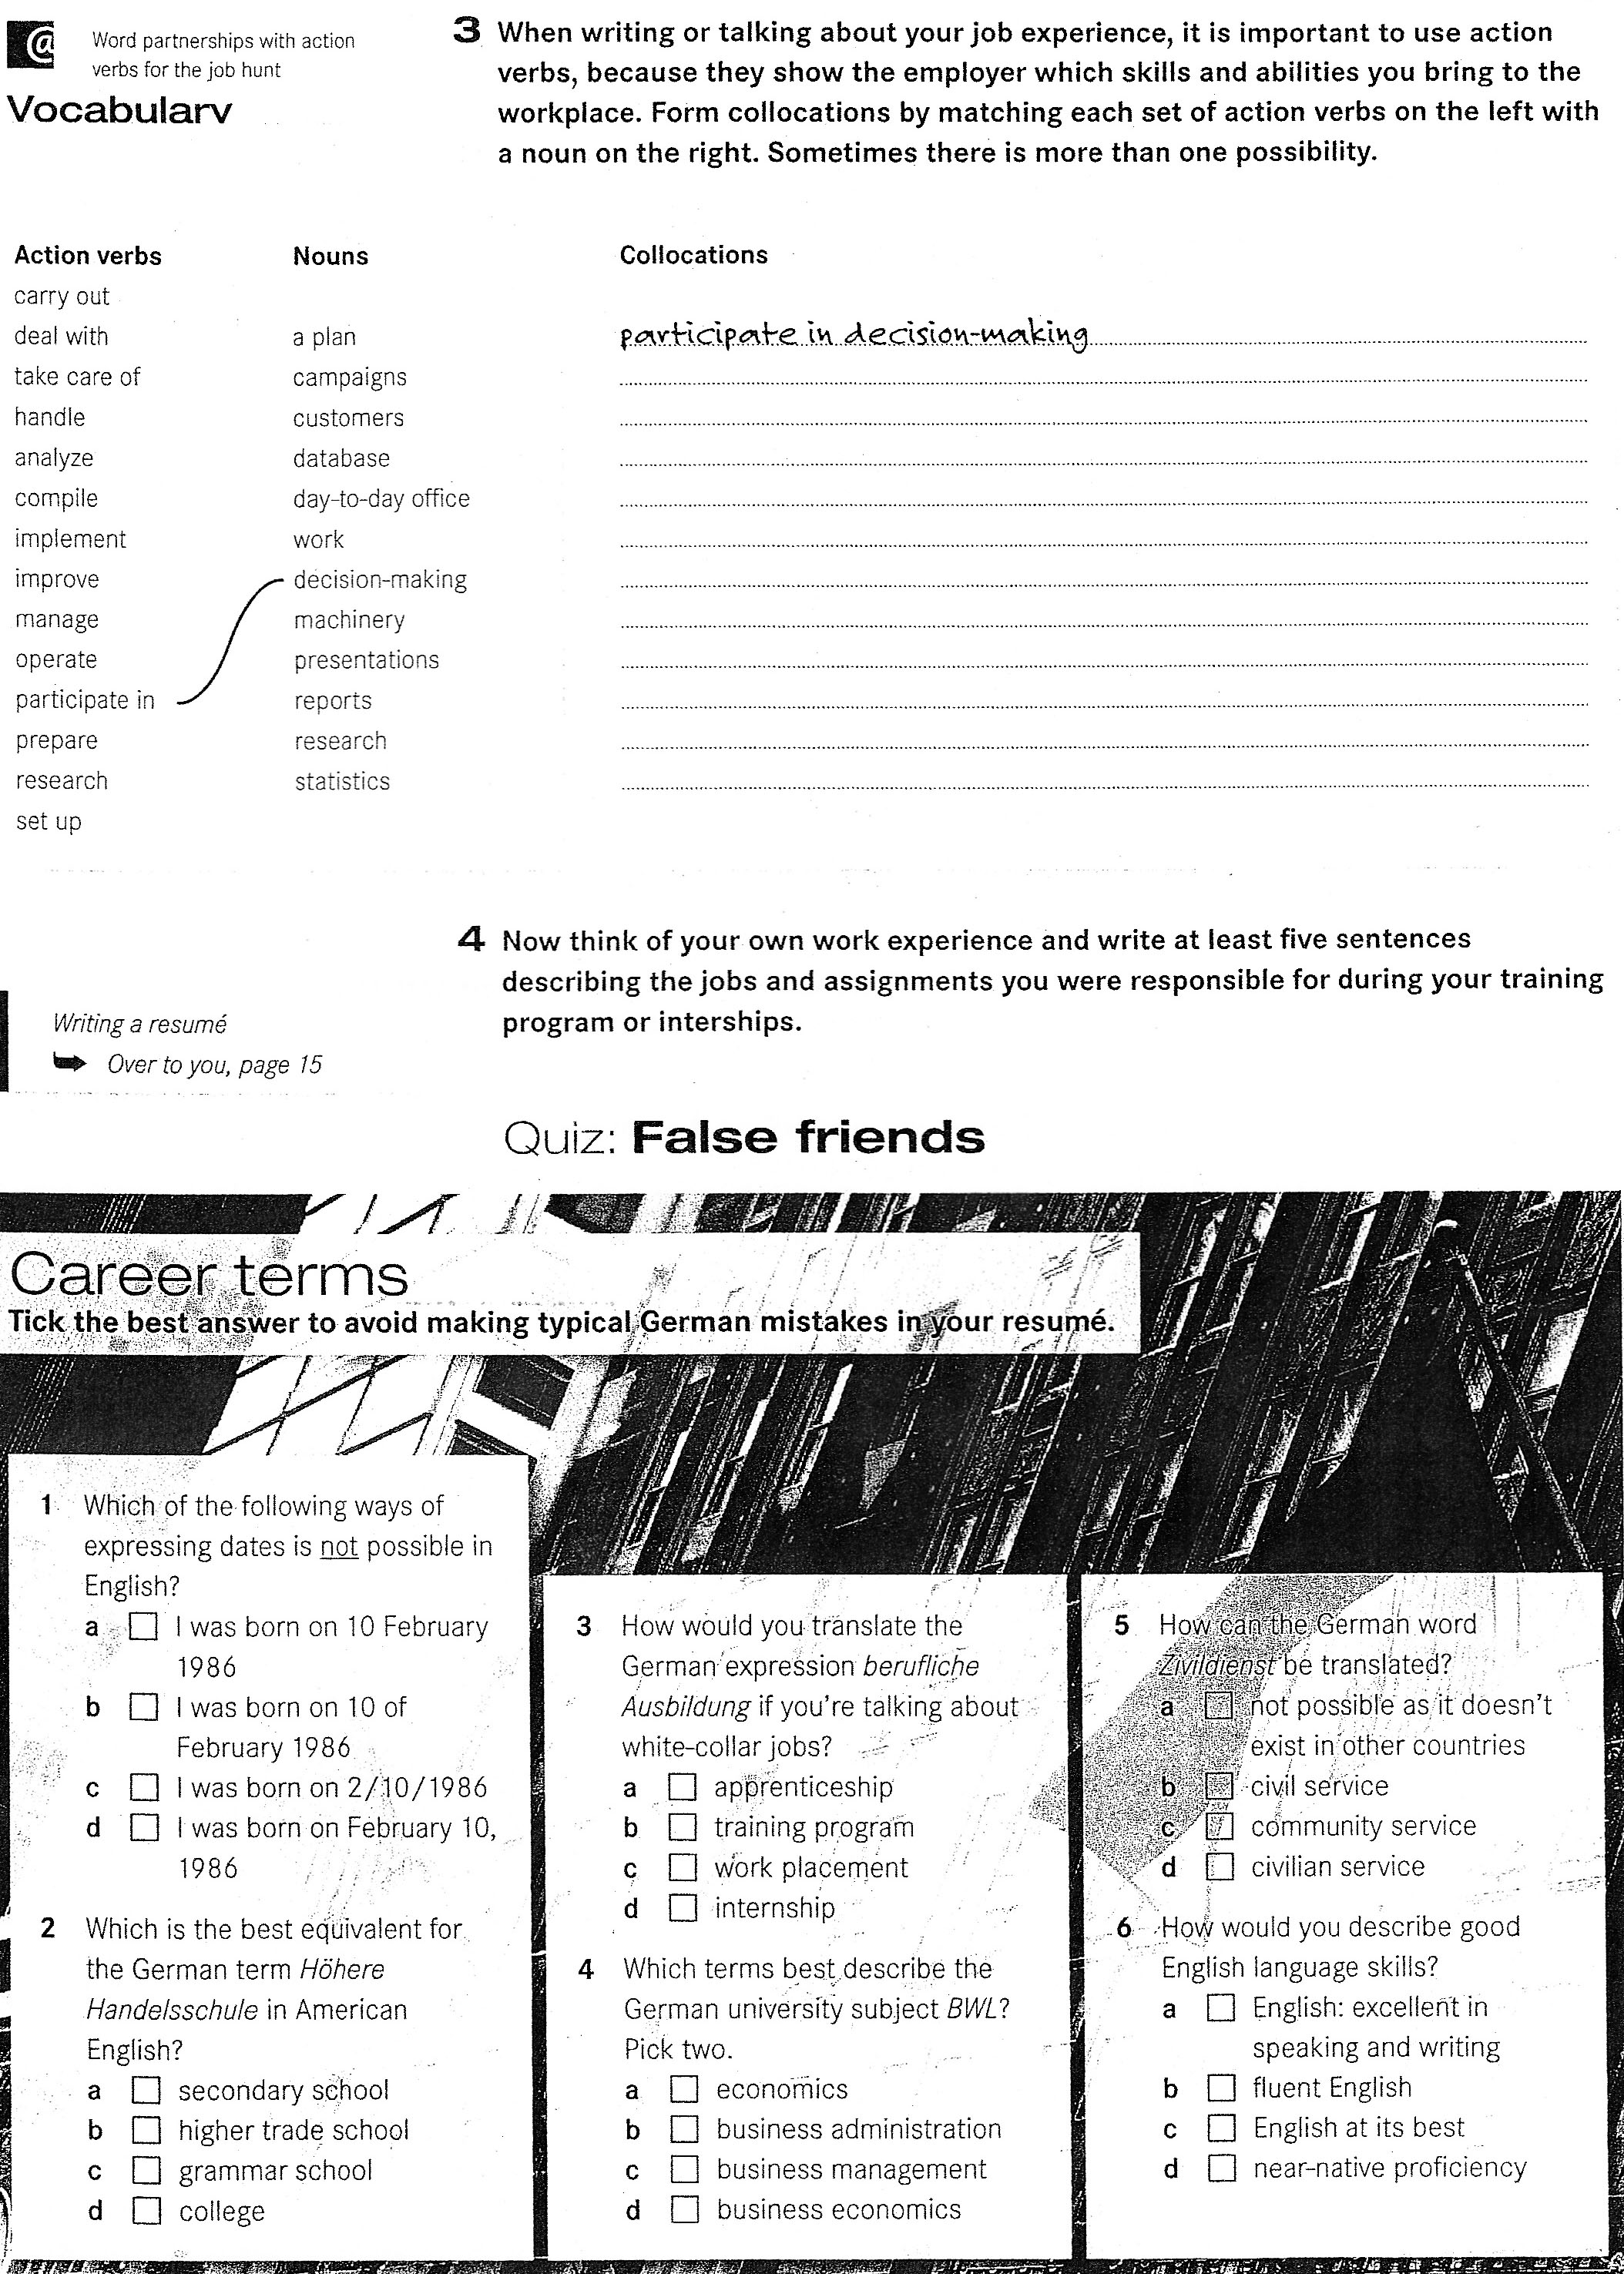
\includegraphics[scale=.85]{handouts/Eng405.jpg}

%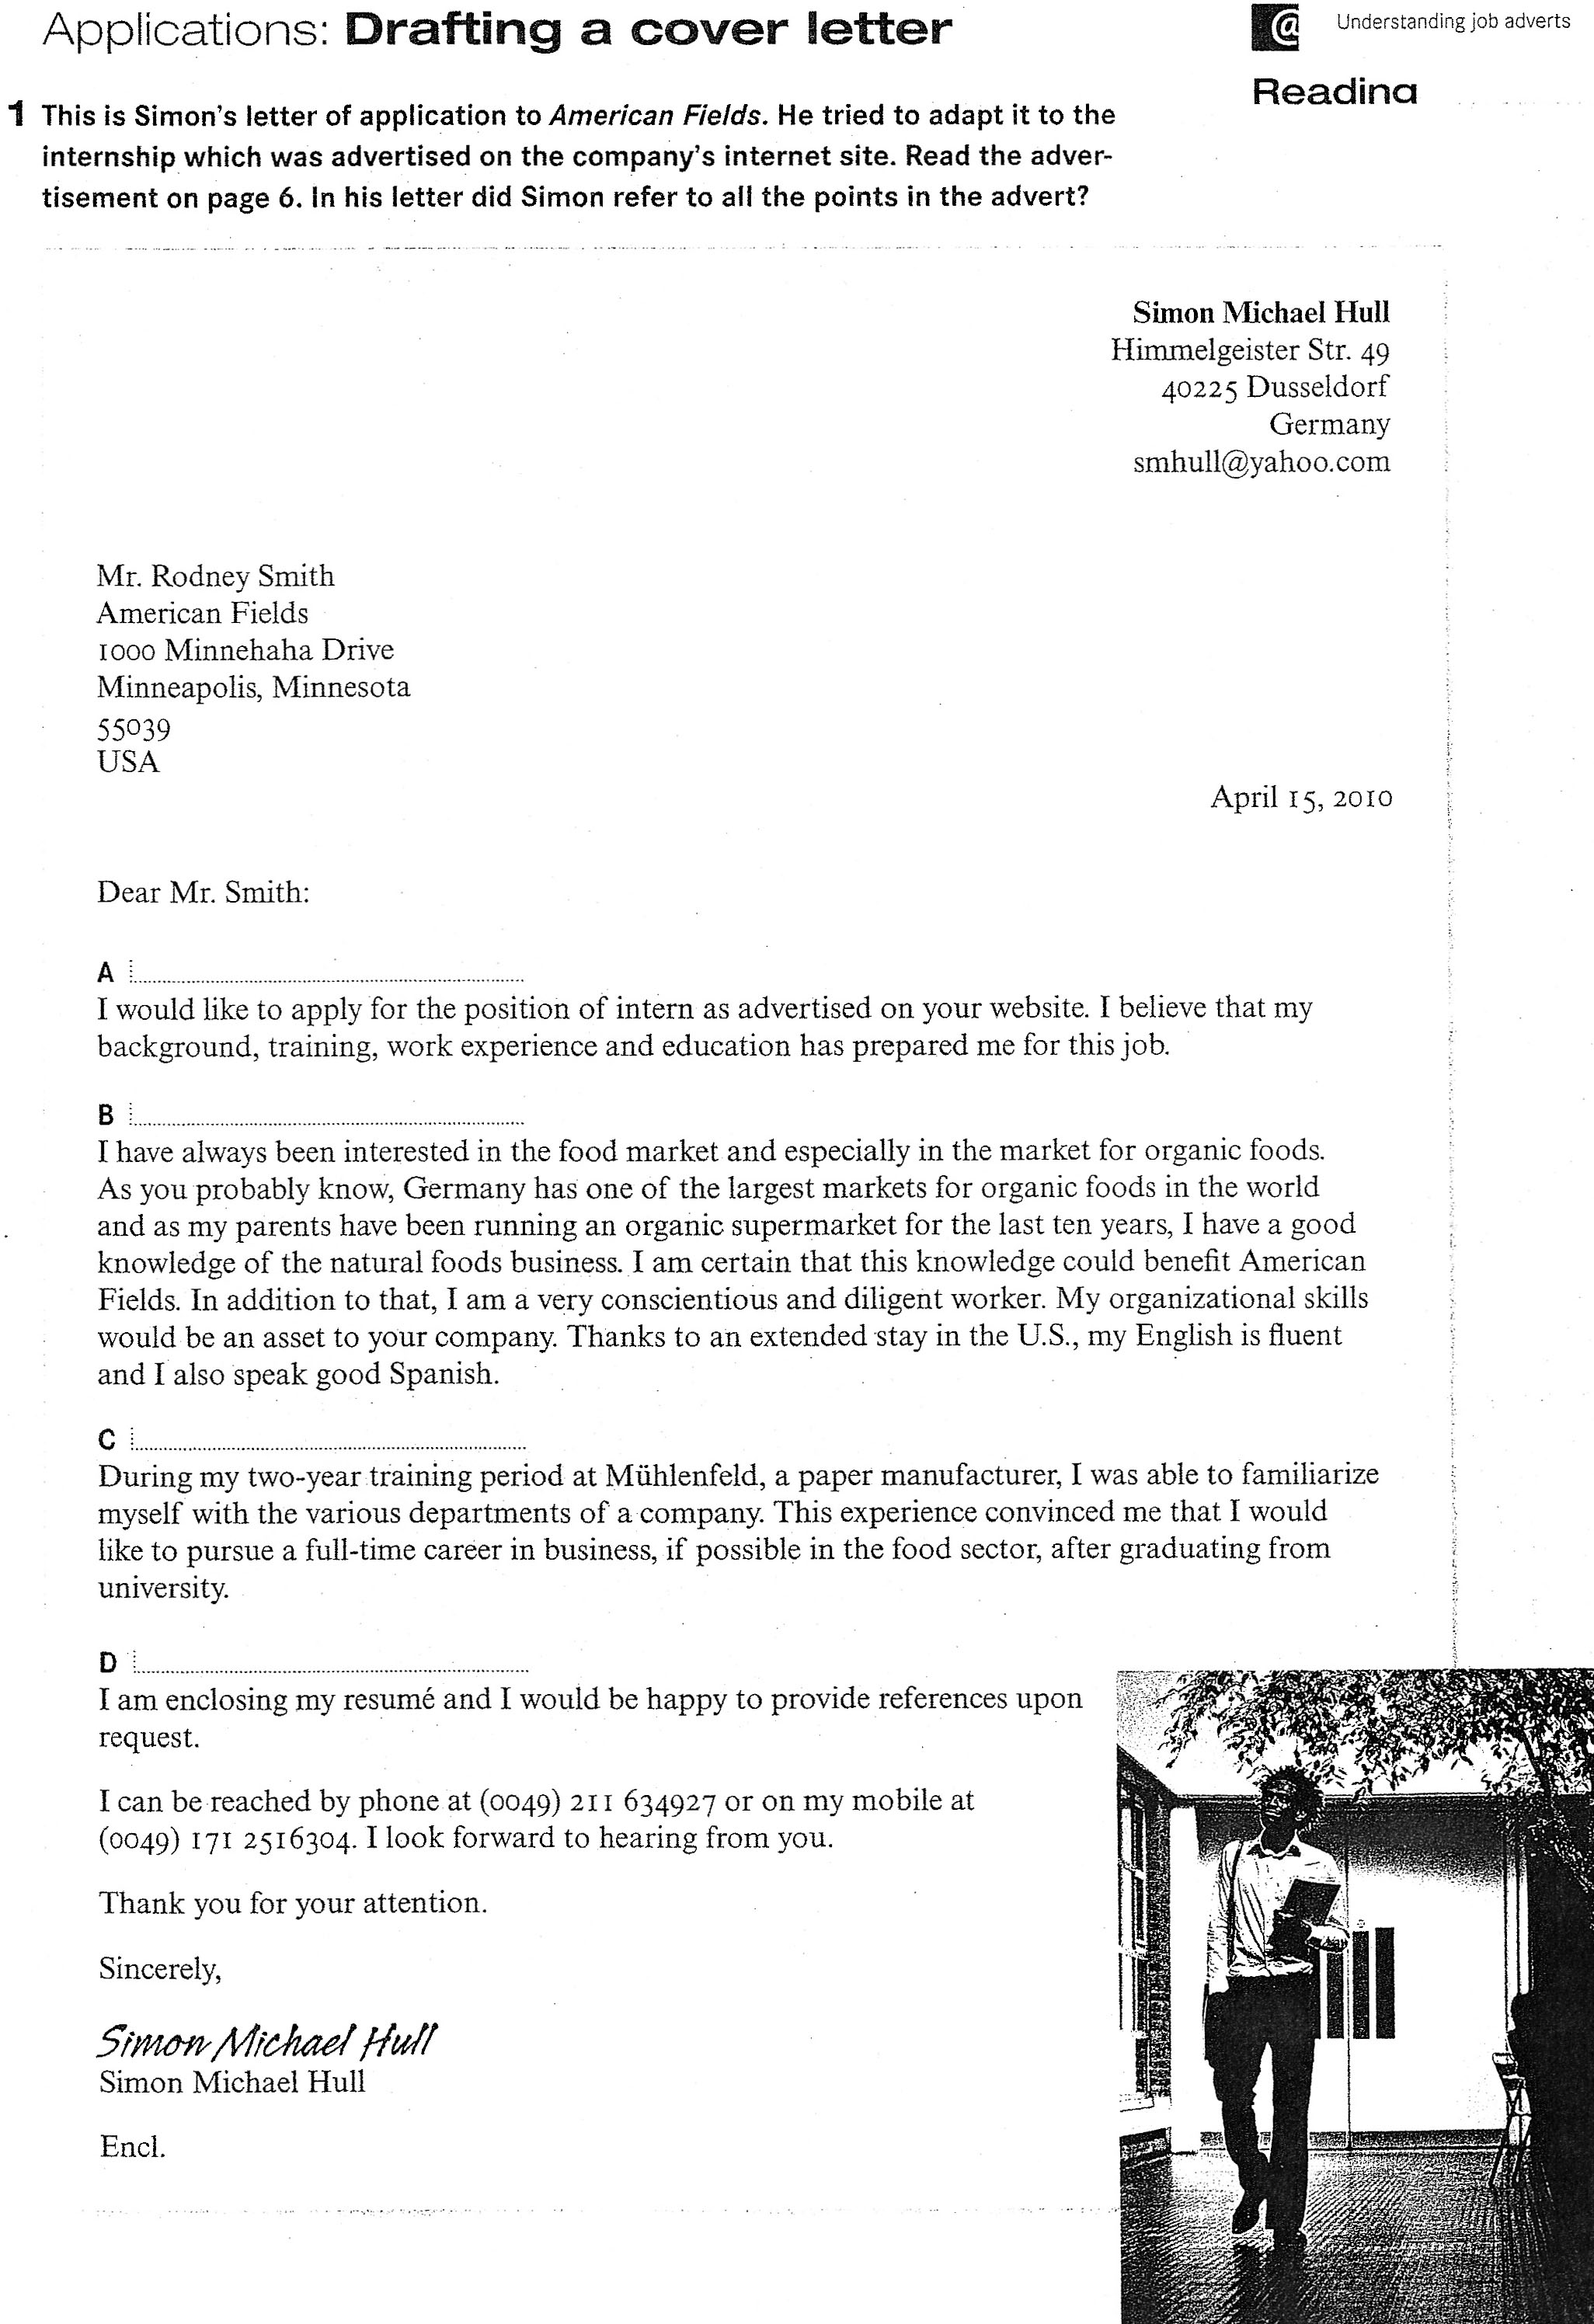
\includegraphics[scale=.85]{handouts/Eng406.jpg}

%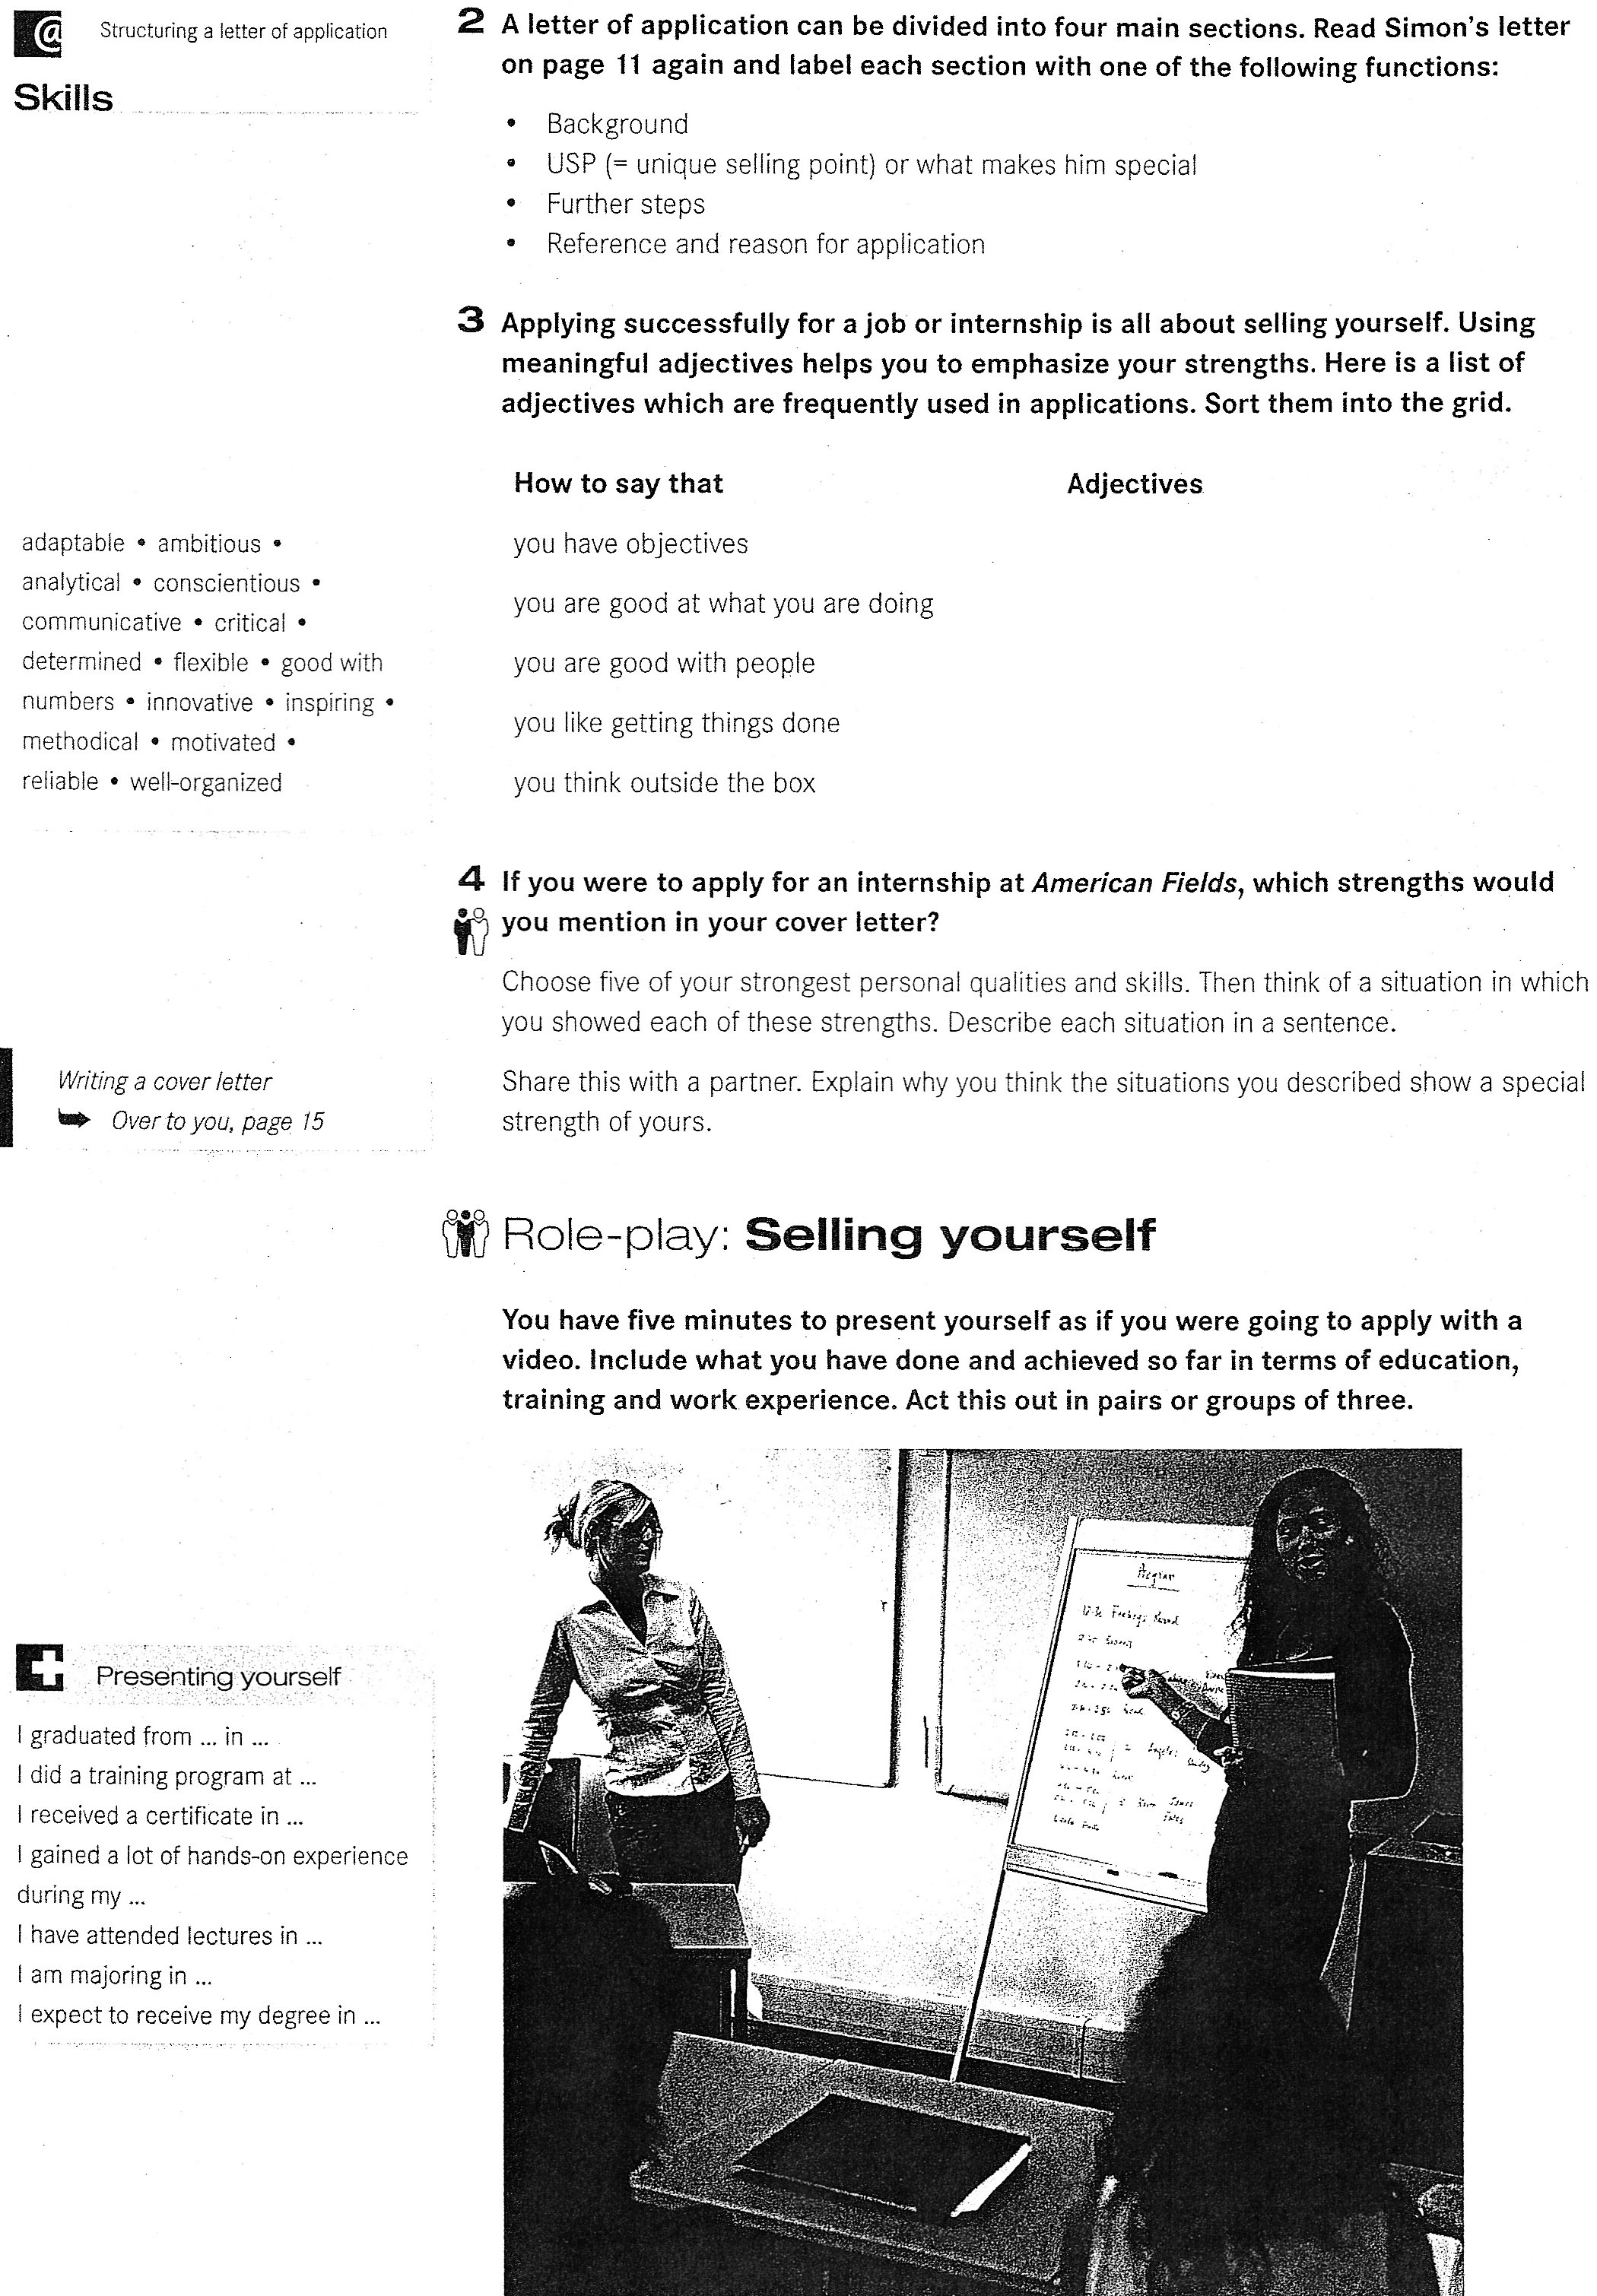
\includegraphics[scale=.85]{handouts/Eng407.jpg}

%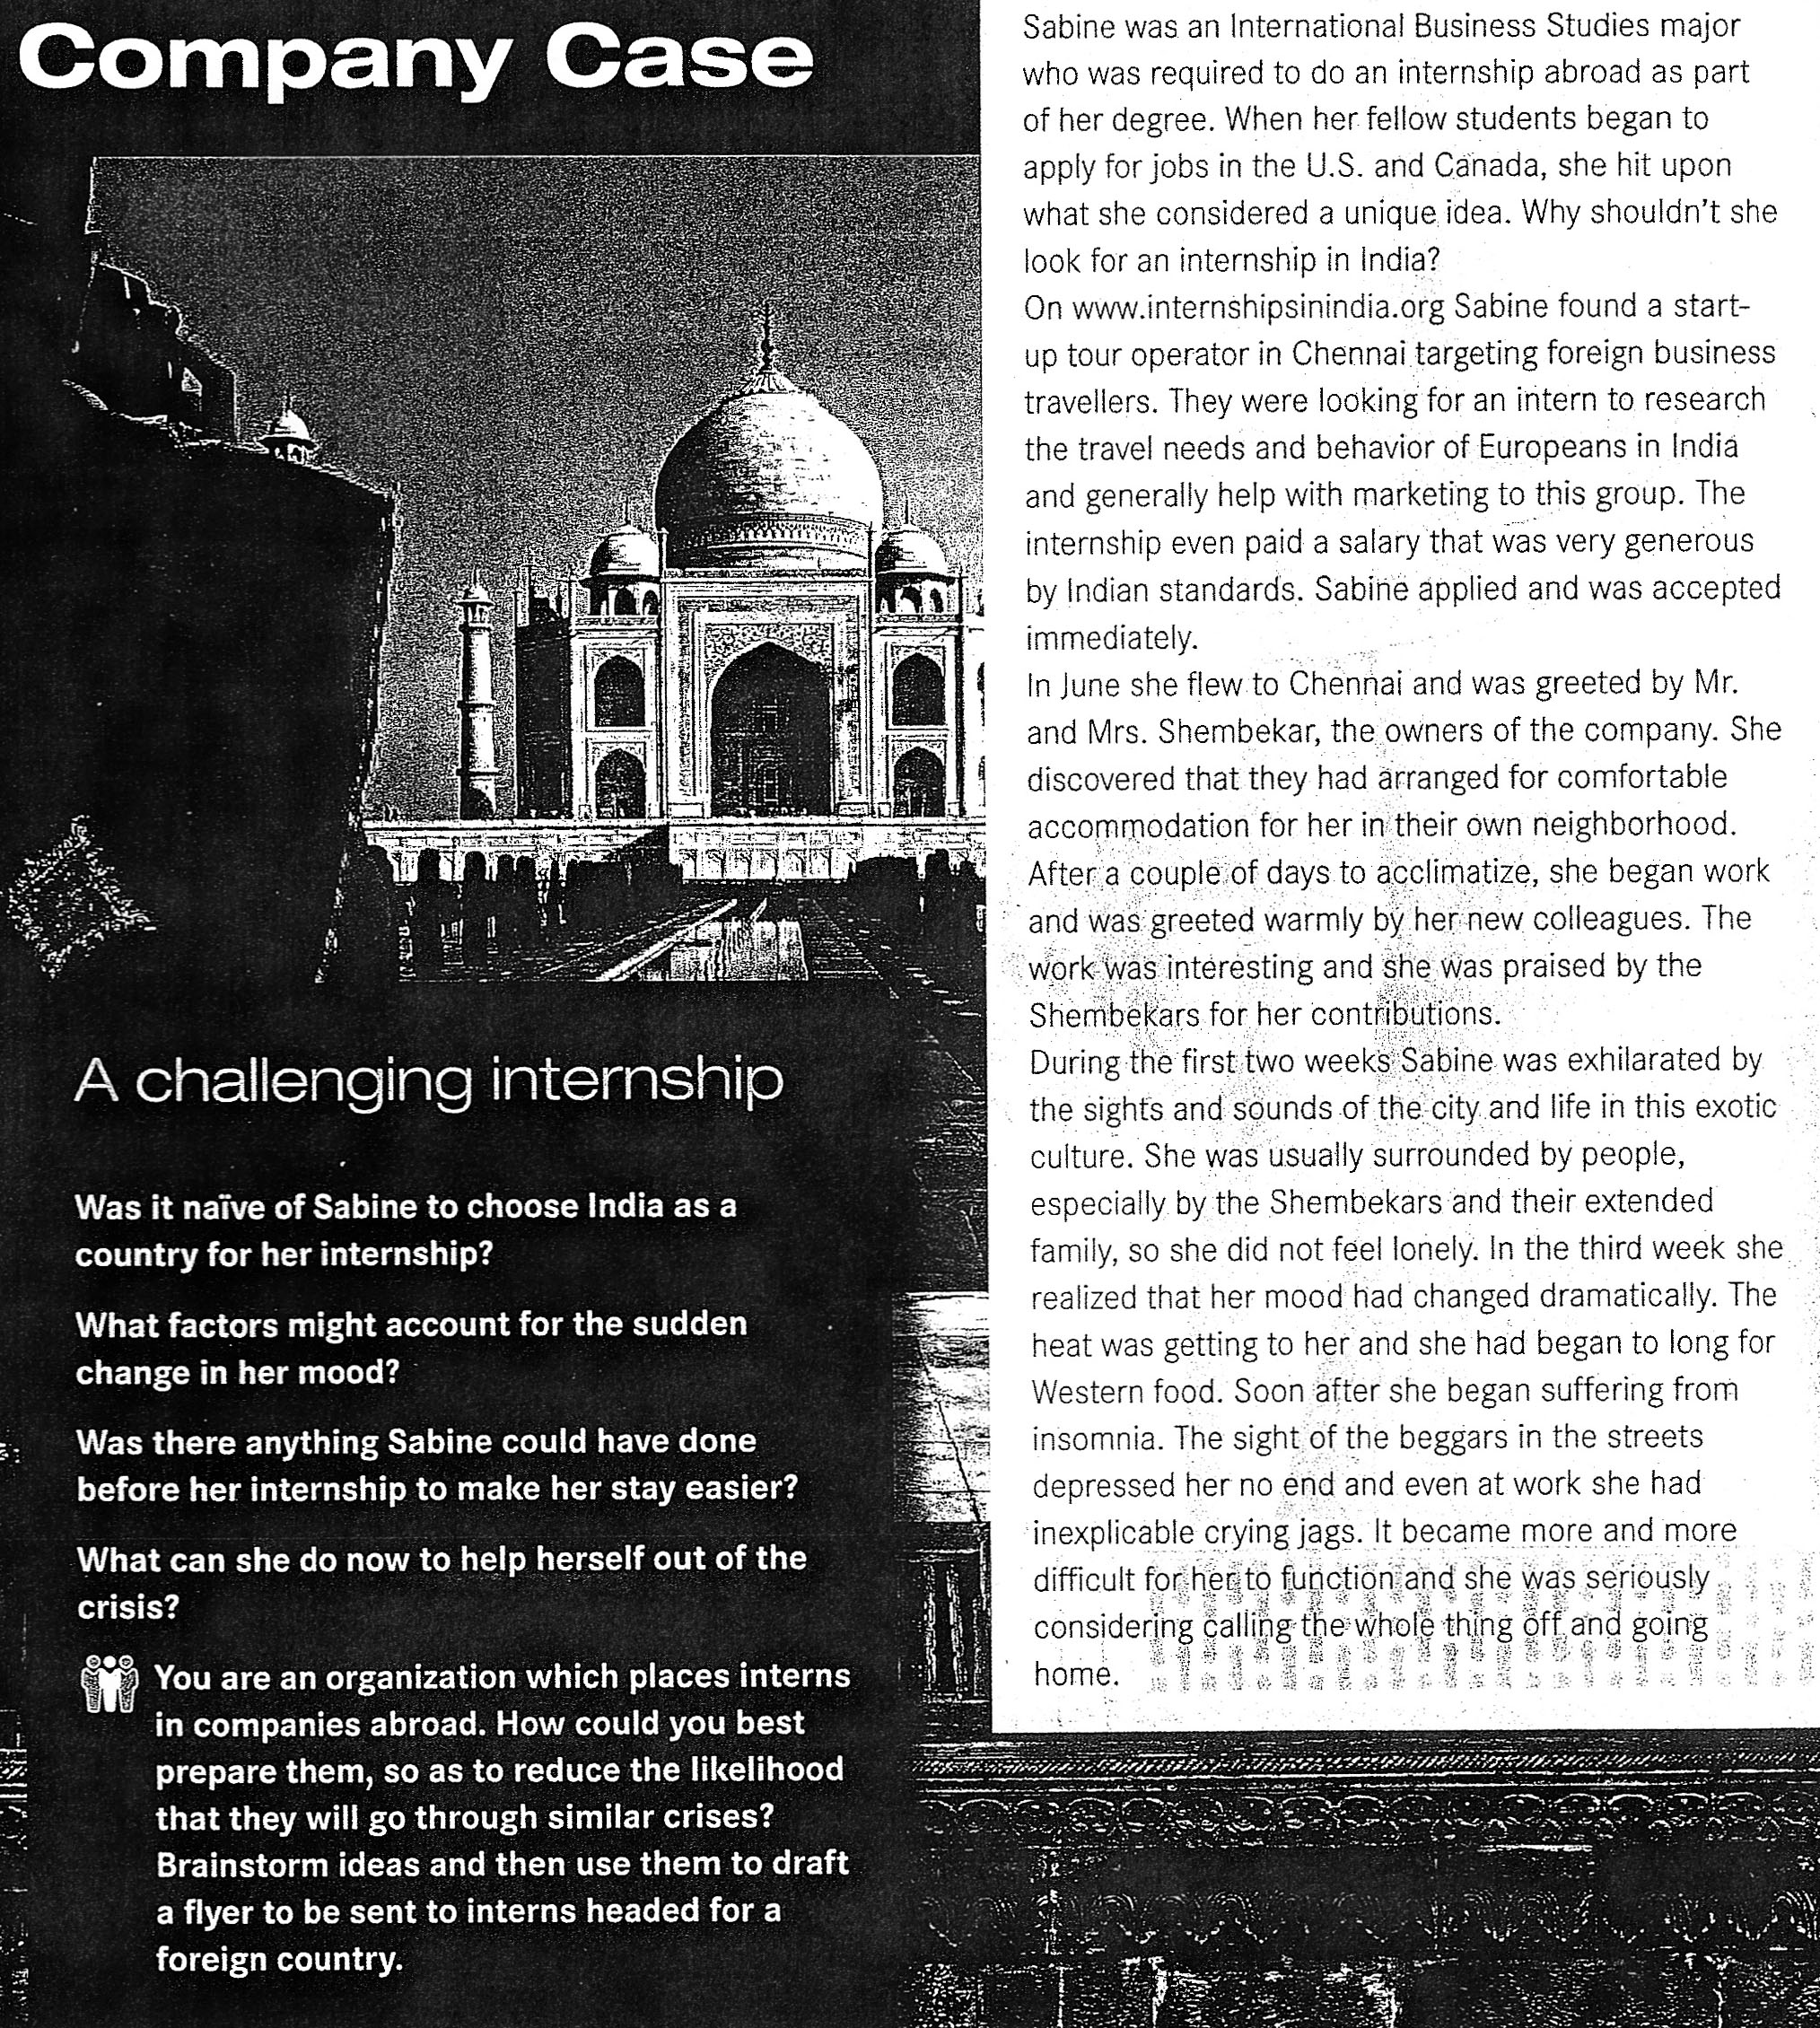
\includegraphics[scale=.85]{handouts/Eng409.jpg}

%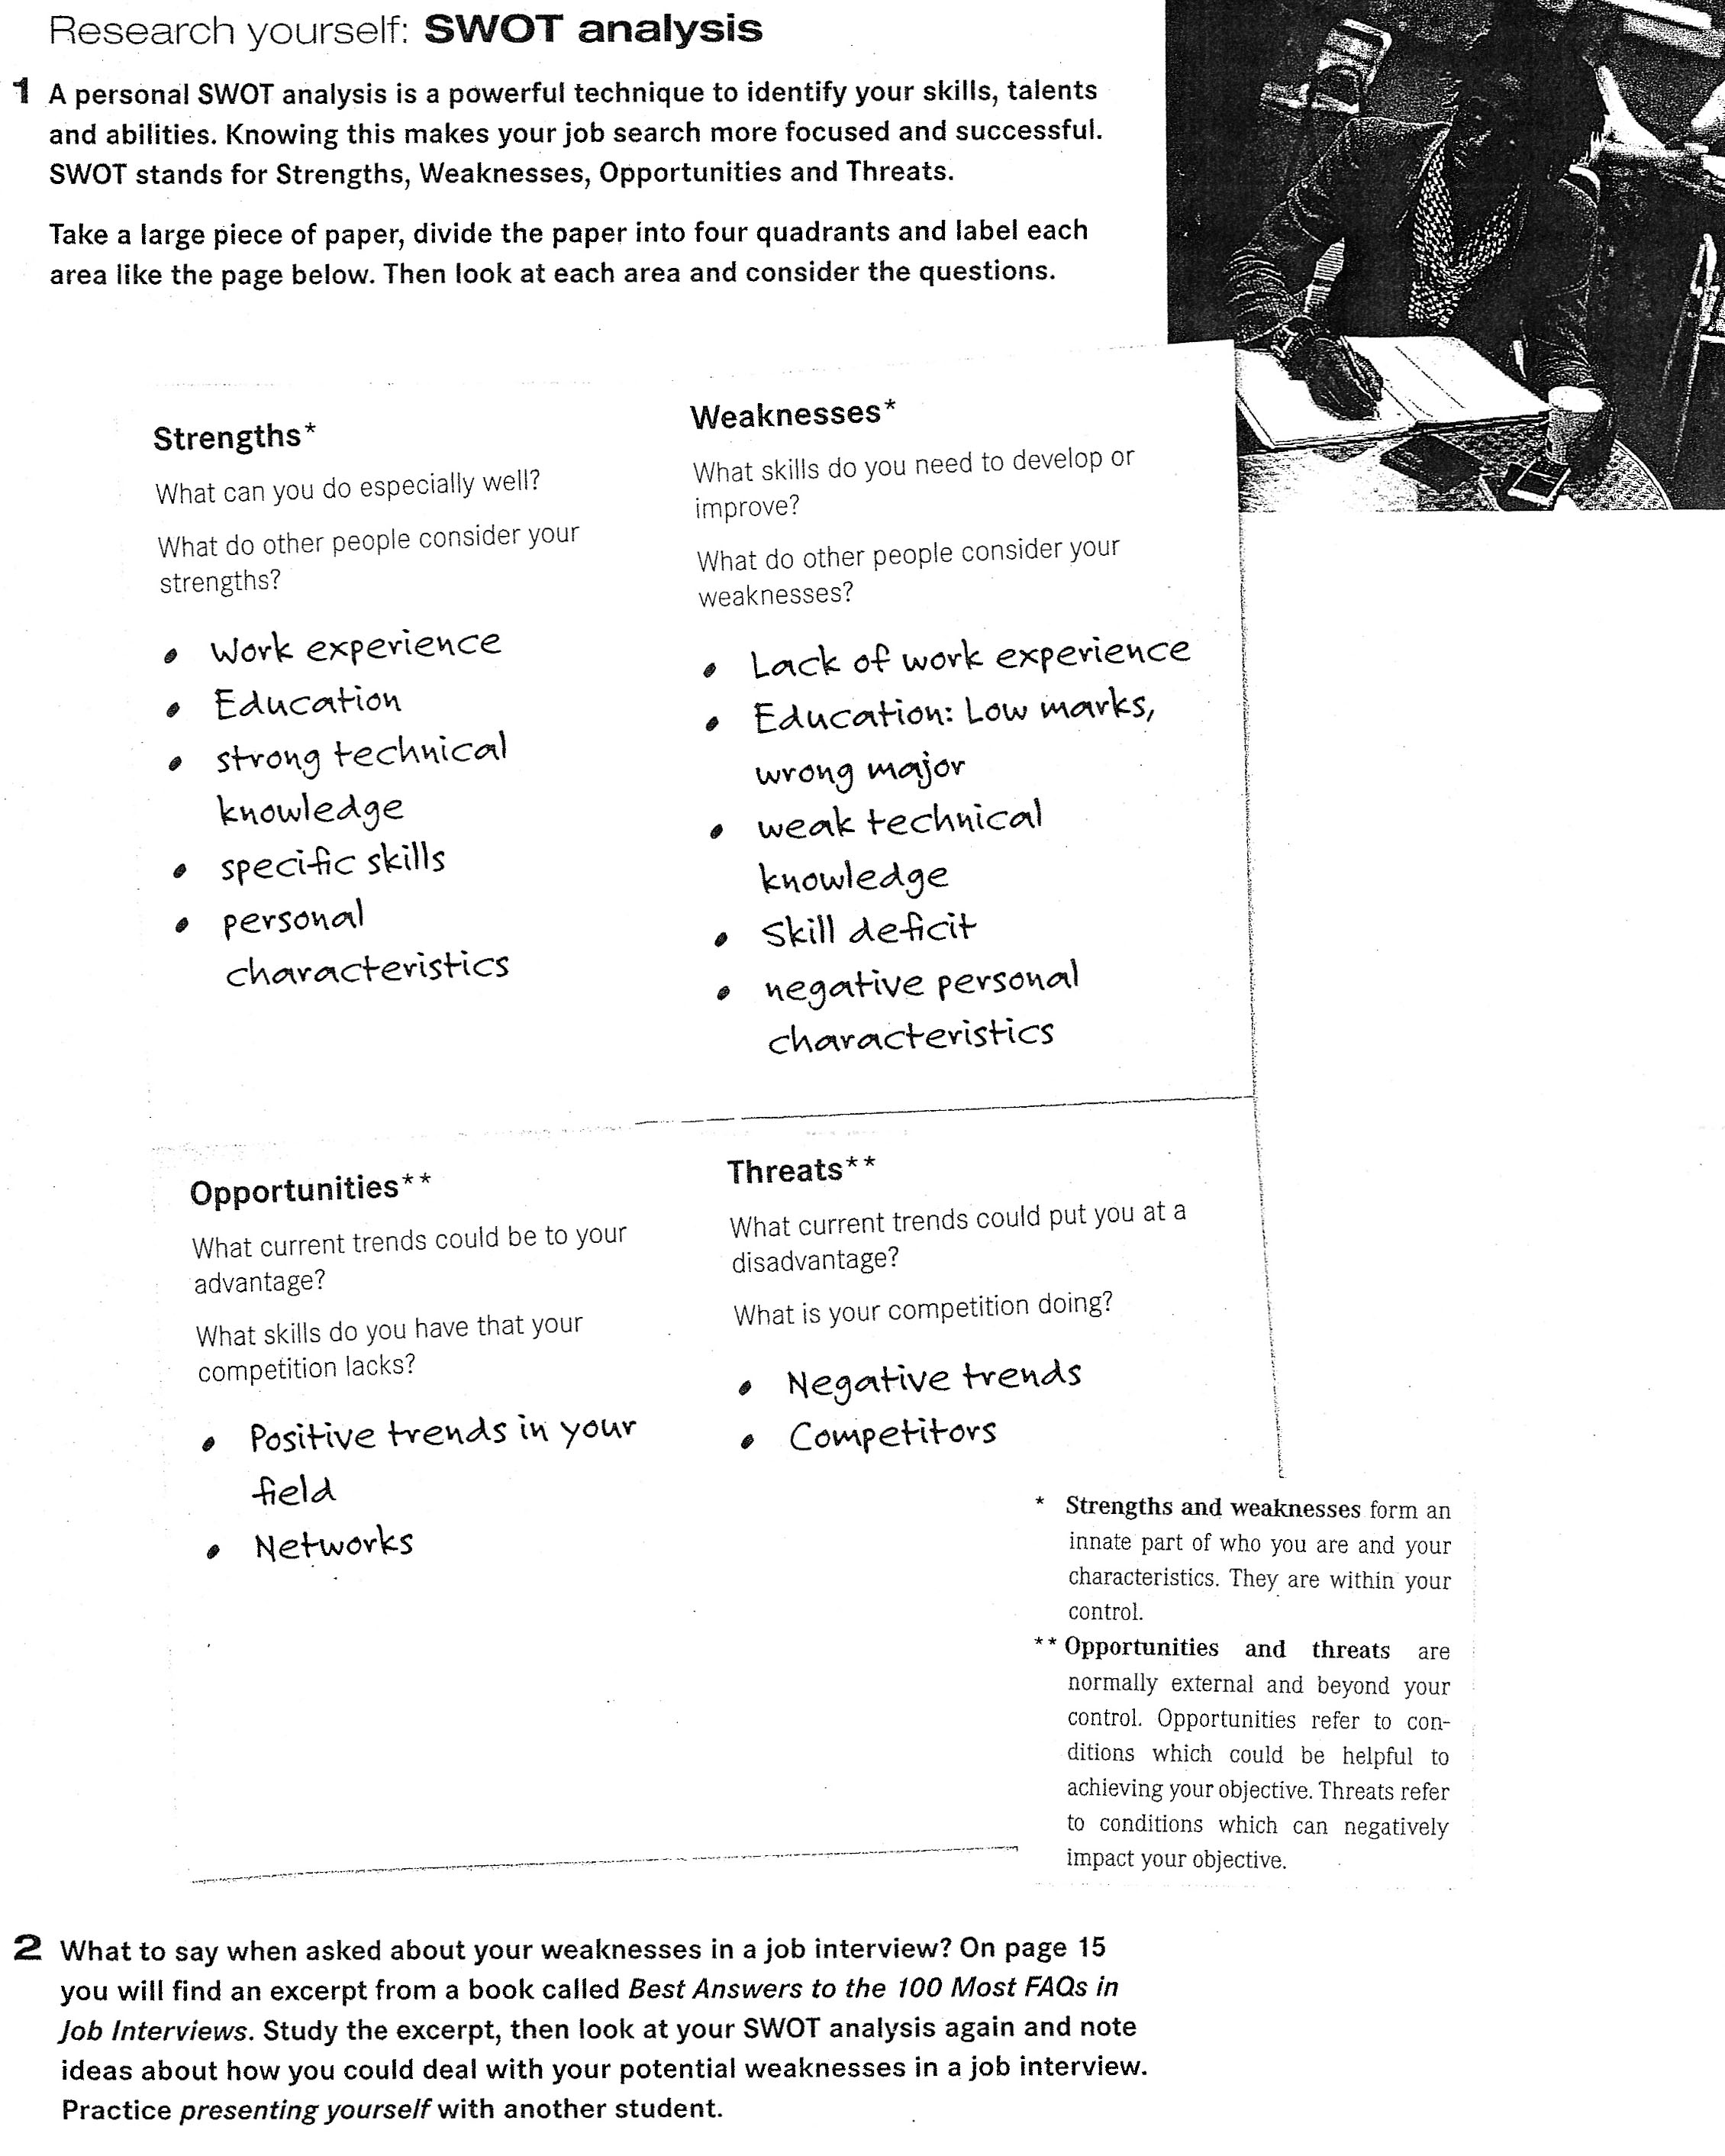
\includegraphics[scale=.85]{handouts/Eng410.jpg}

%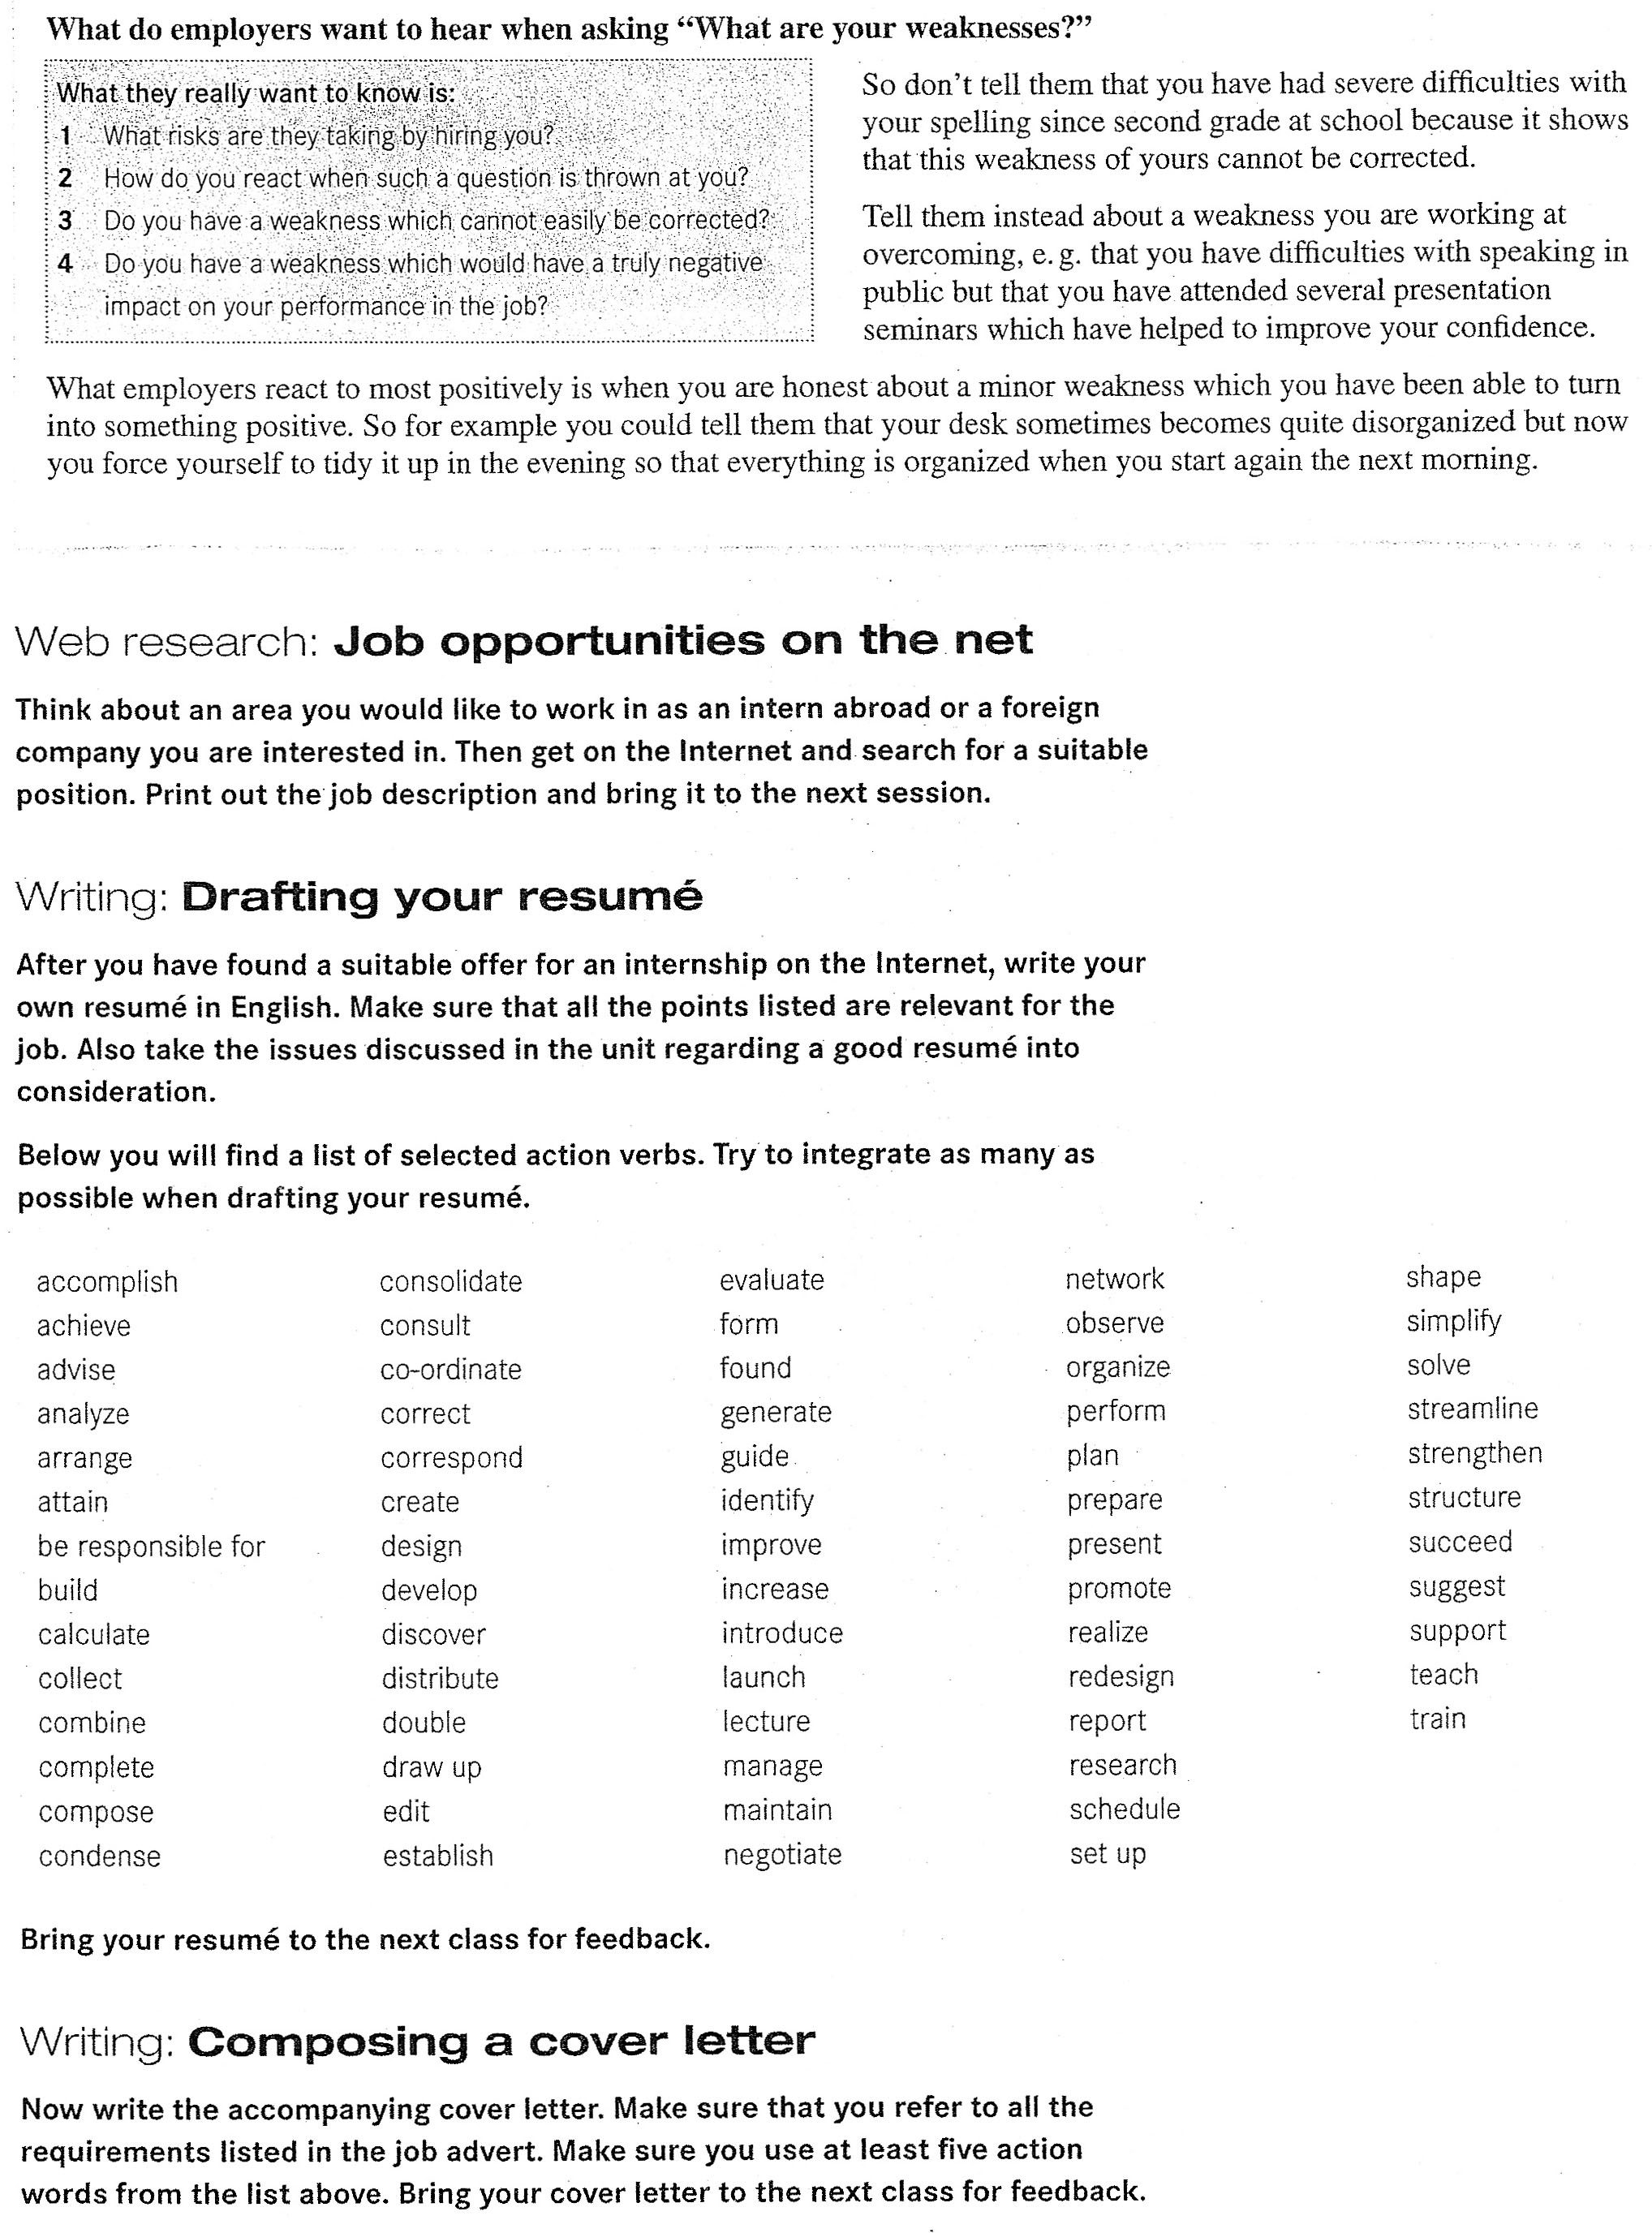
\includegraphics[scale=.85]{handouts/Eng408.jpg}

\chapter{Job Applications}
Berkley%\\
%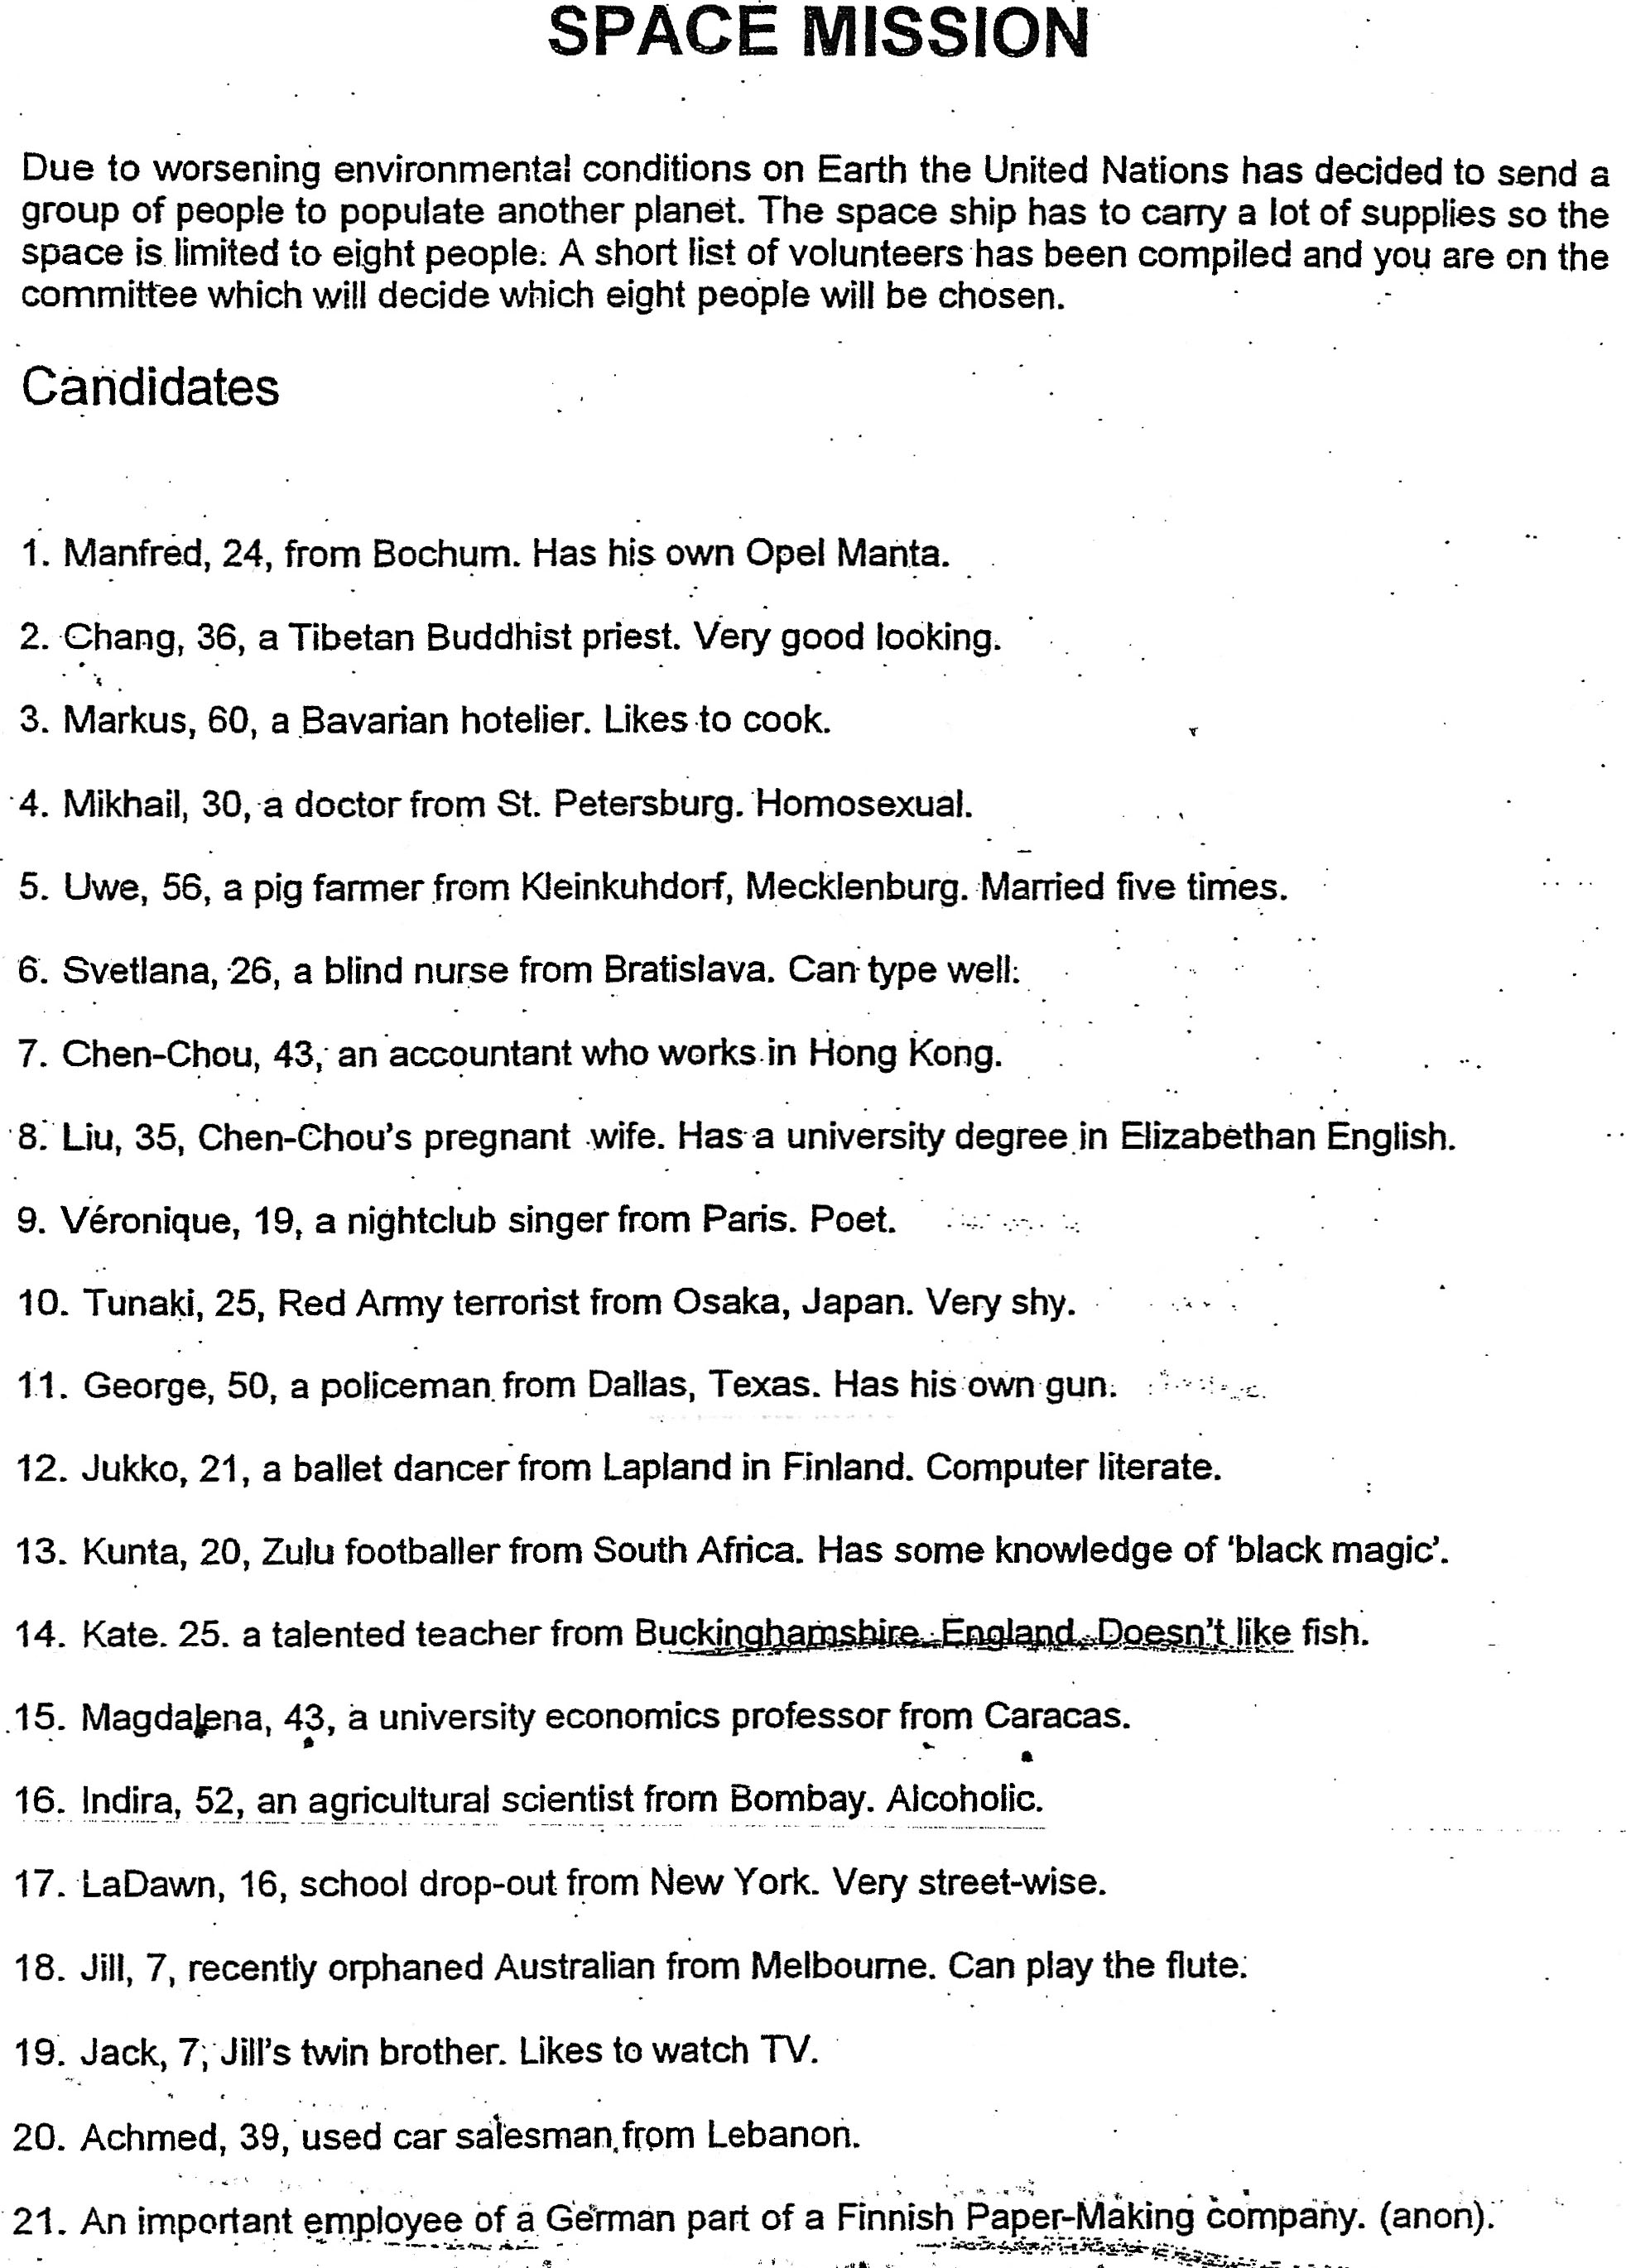
\includegraphics[scale=.85]{handouts/Eng501.jpg}
\section{Common interview questions}
%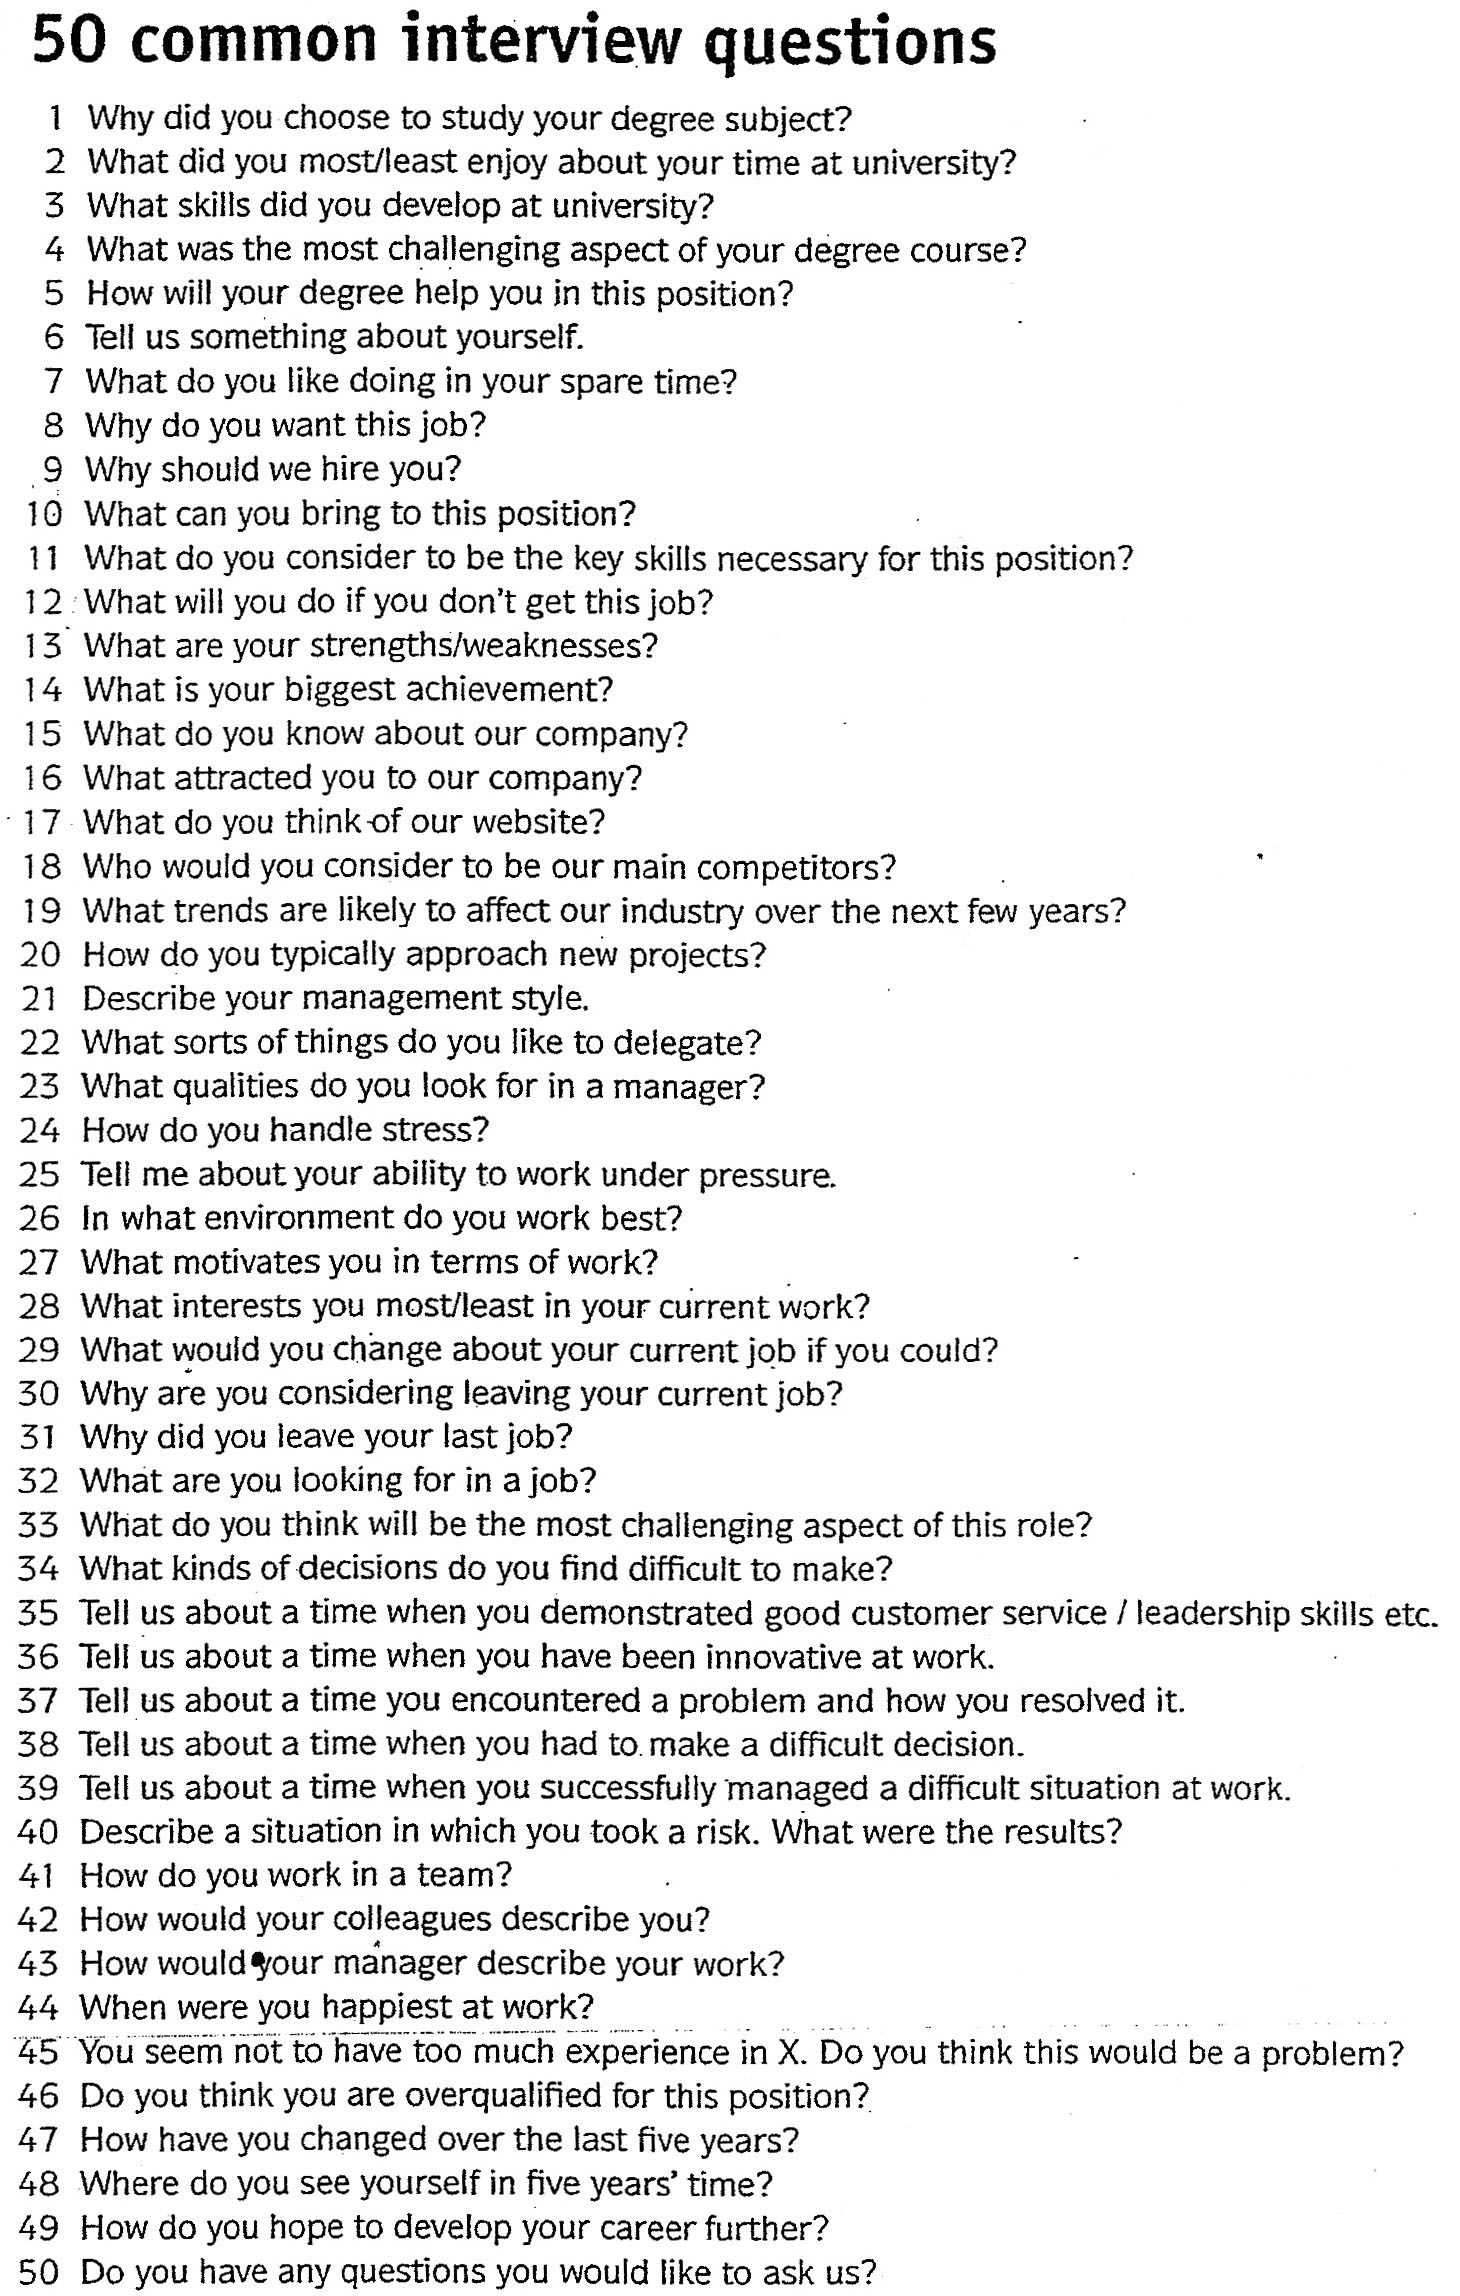
\includegraphics[scale=.85]{handouts/Eng502.jpg}
\section{Asking and answering questions}
%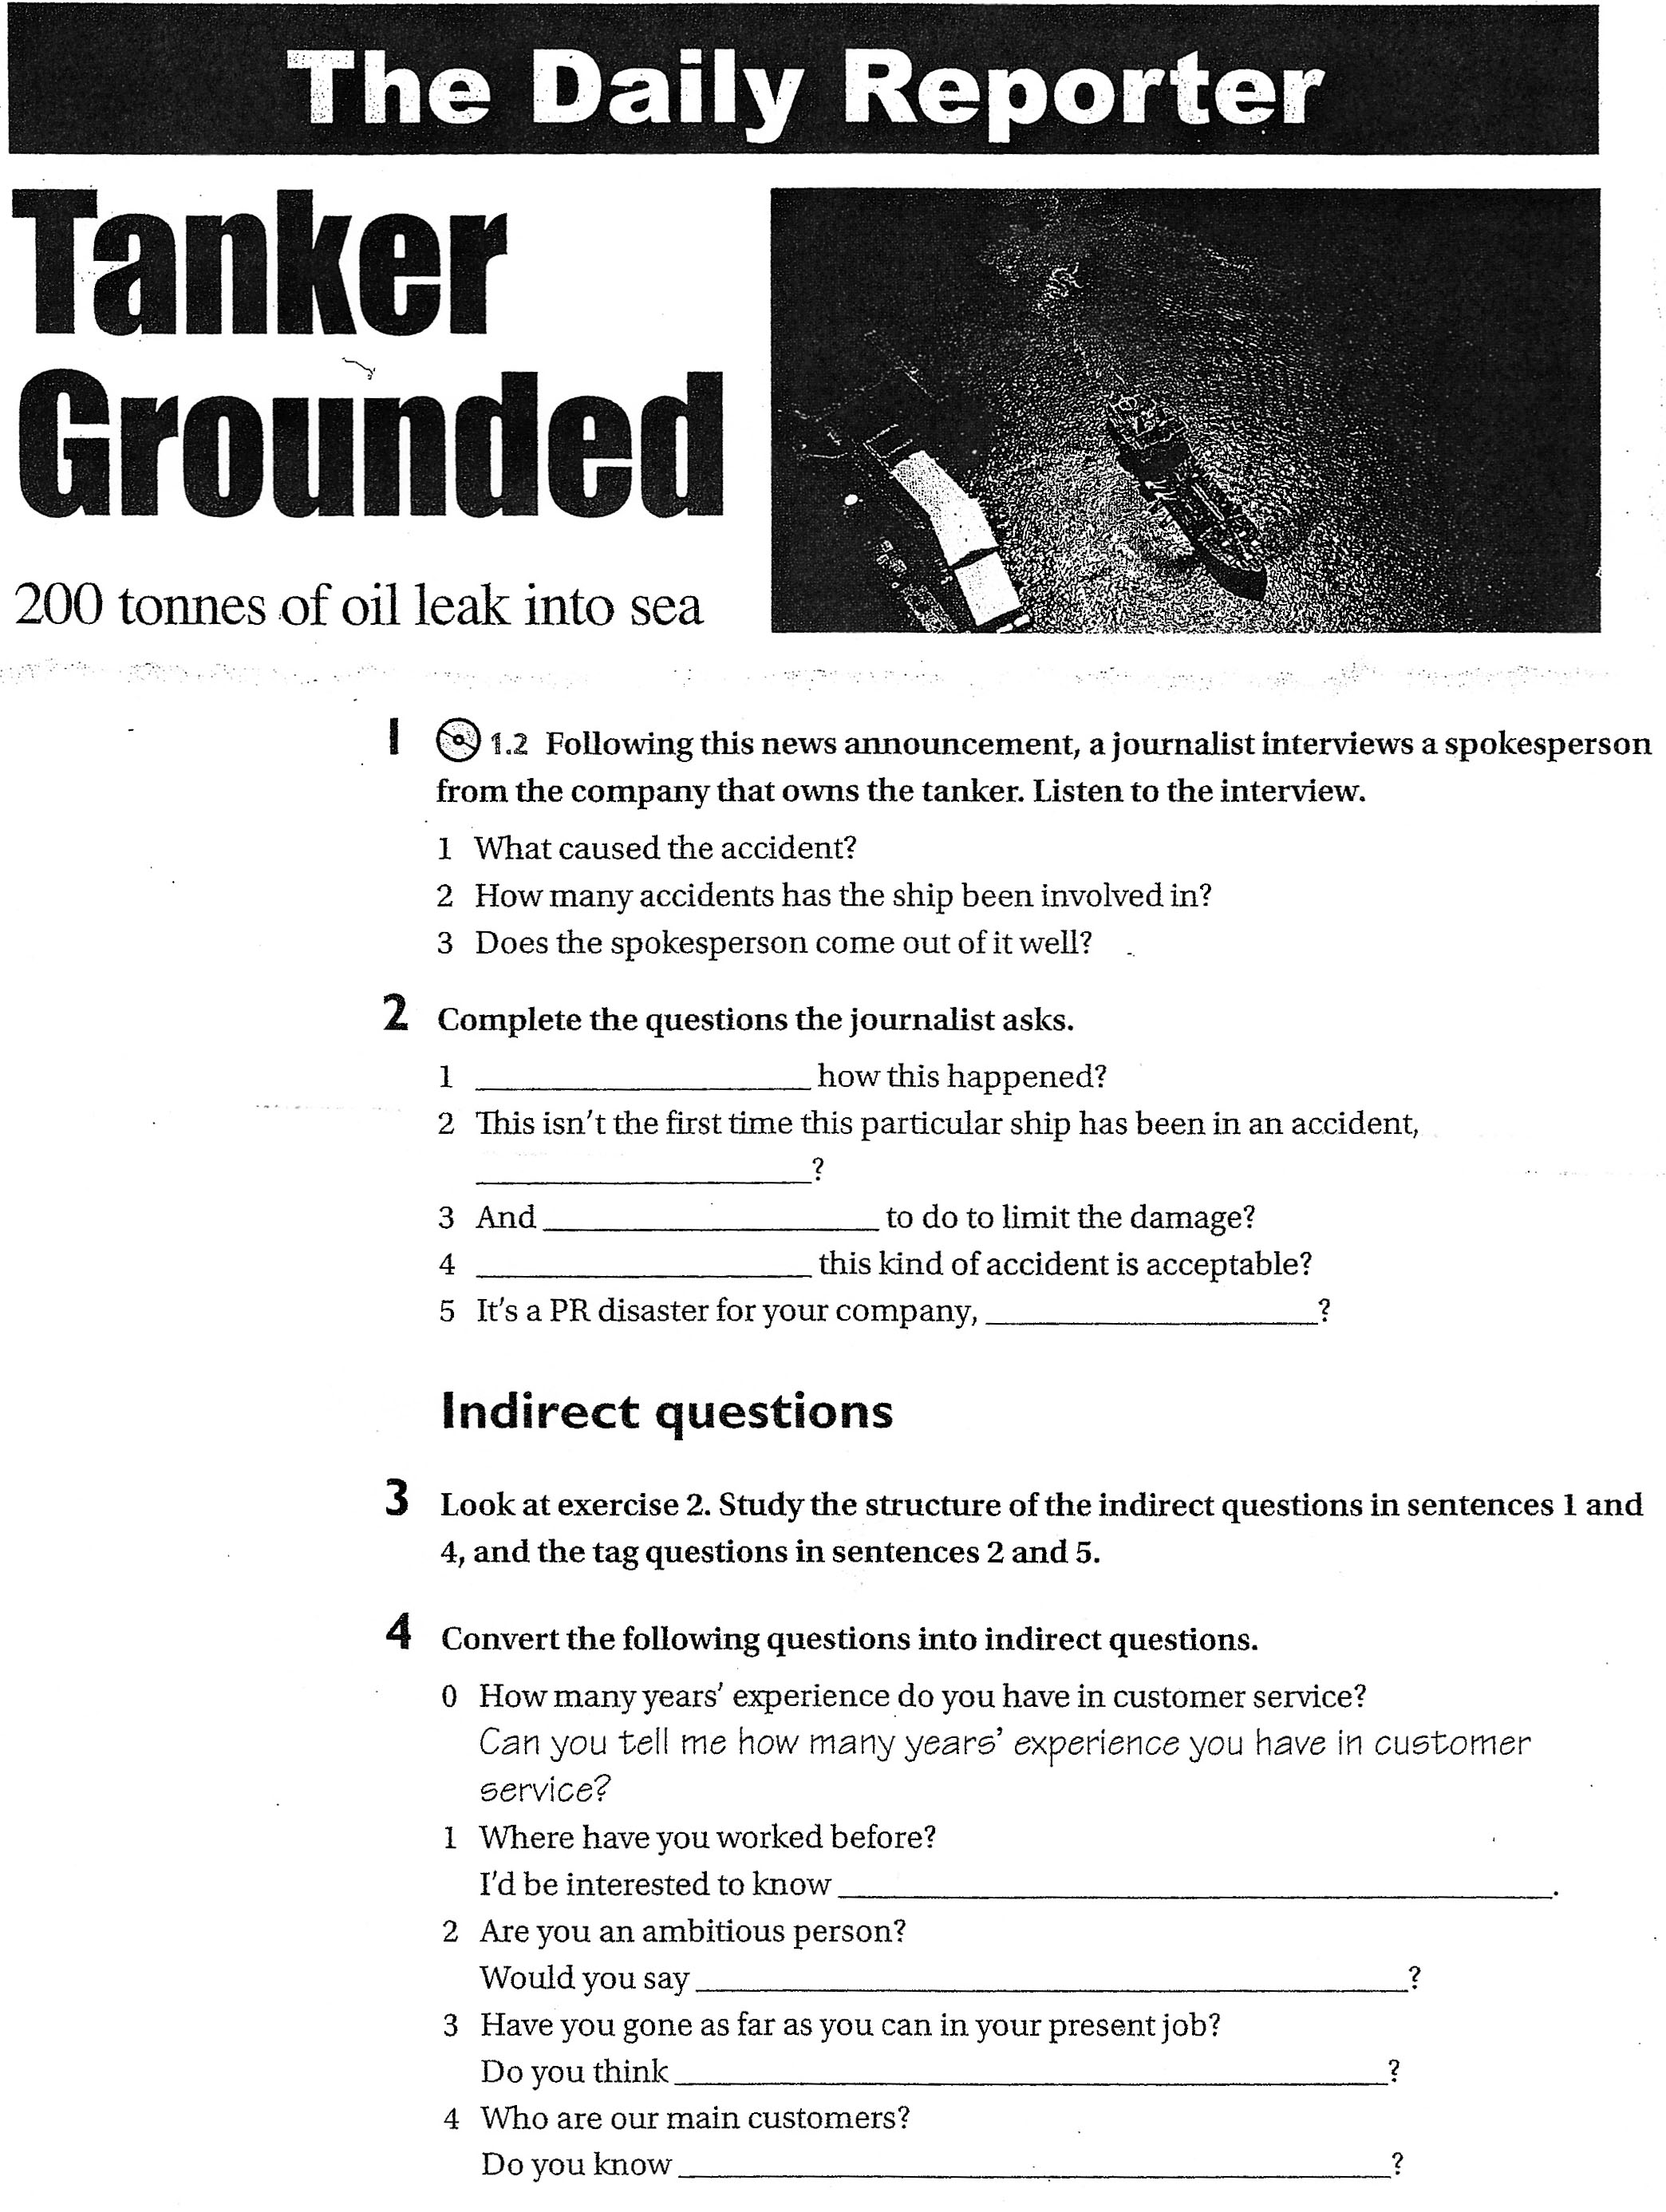
\includegraphics[scale=.85]{handouts/Eng503.jpg}

%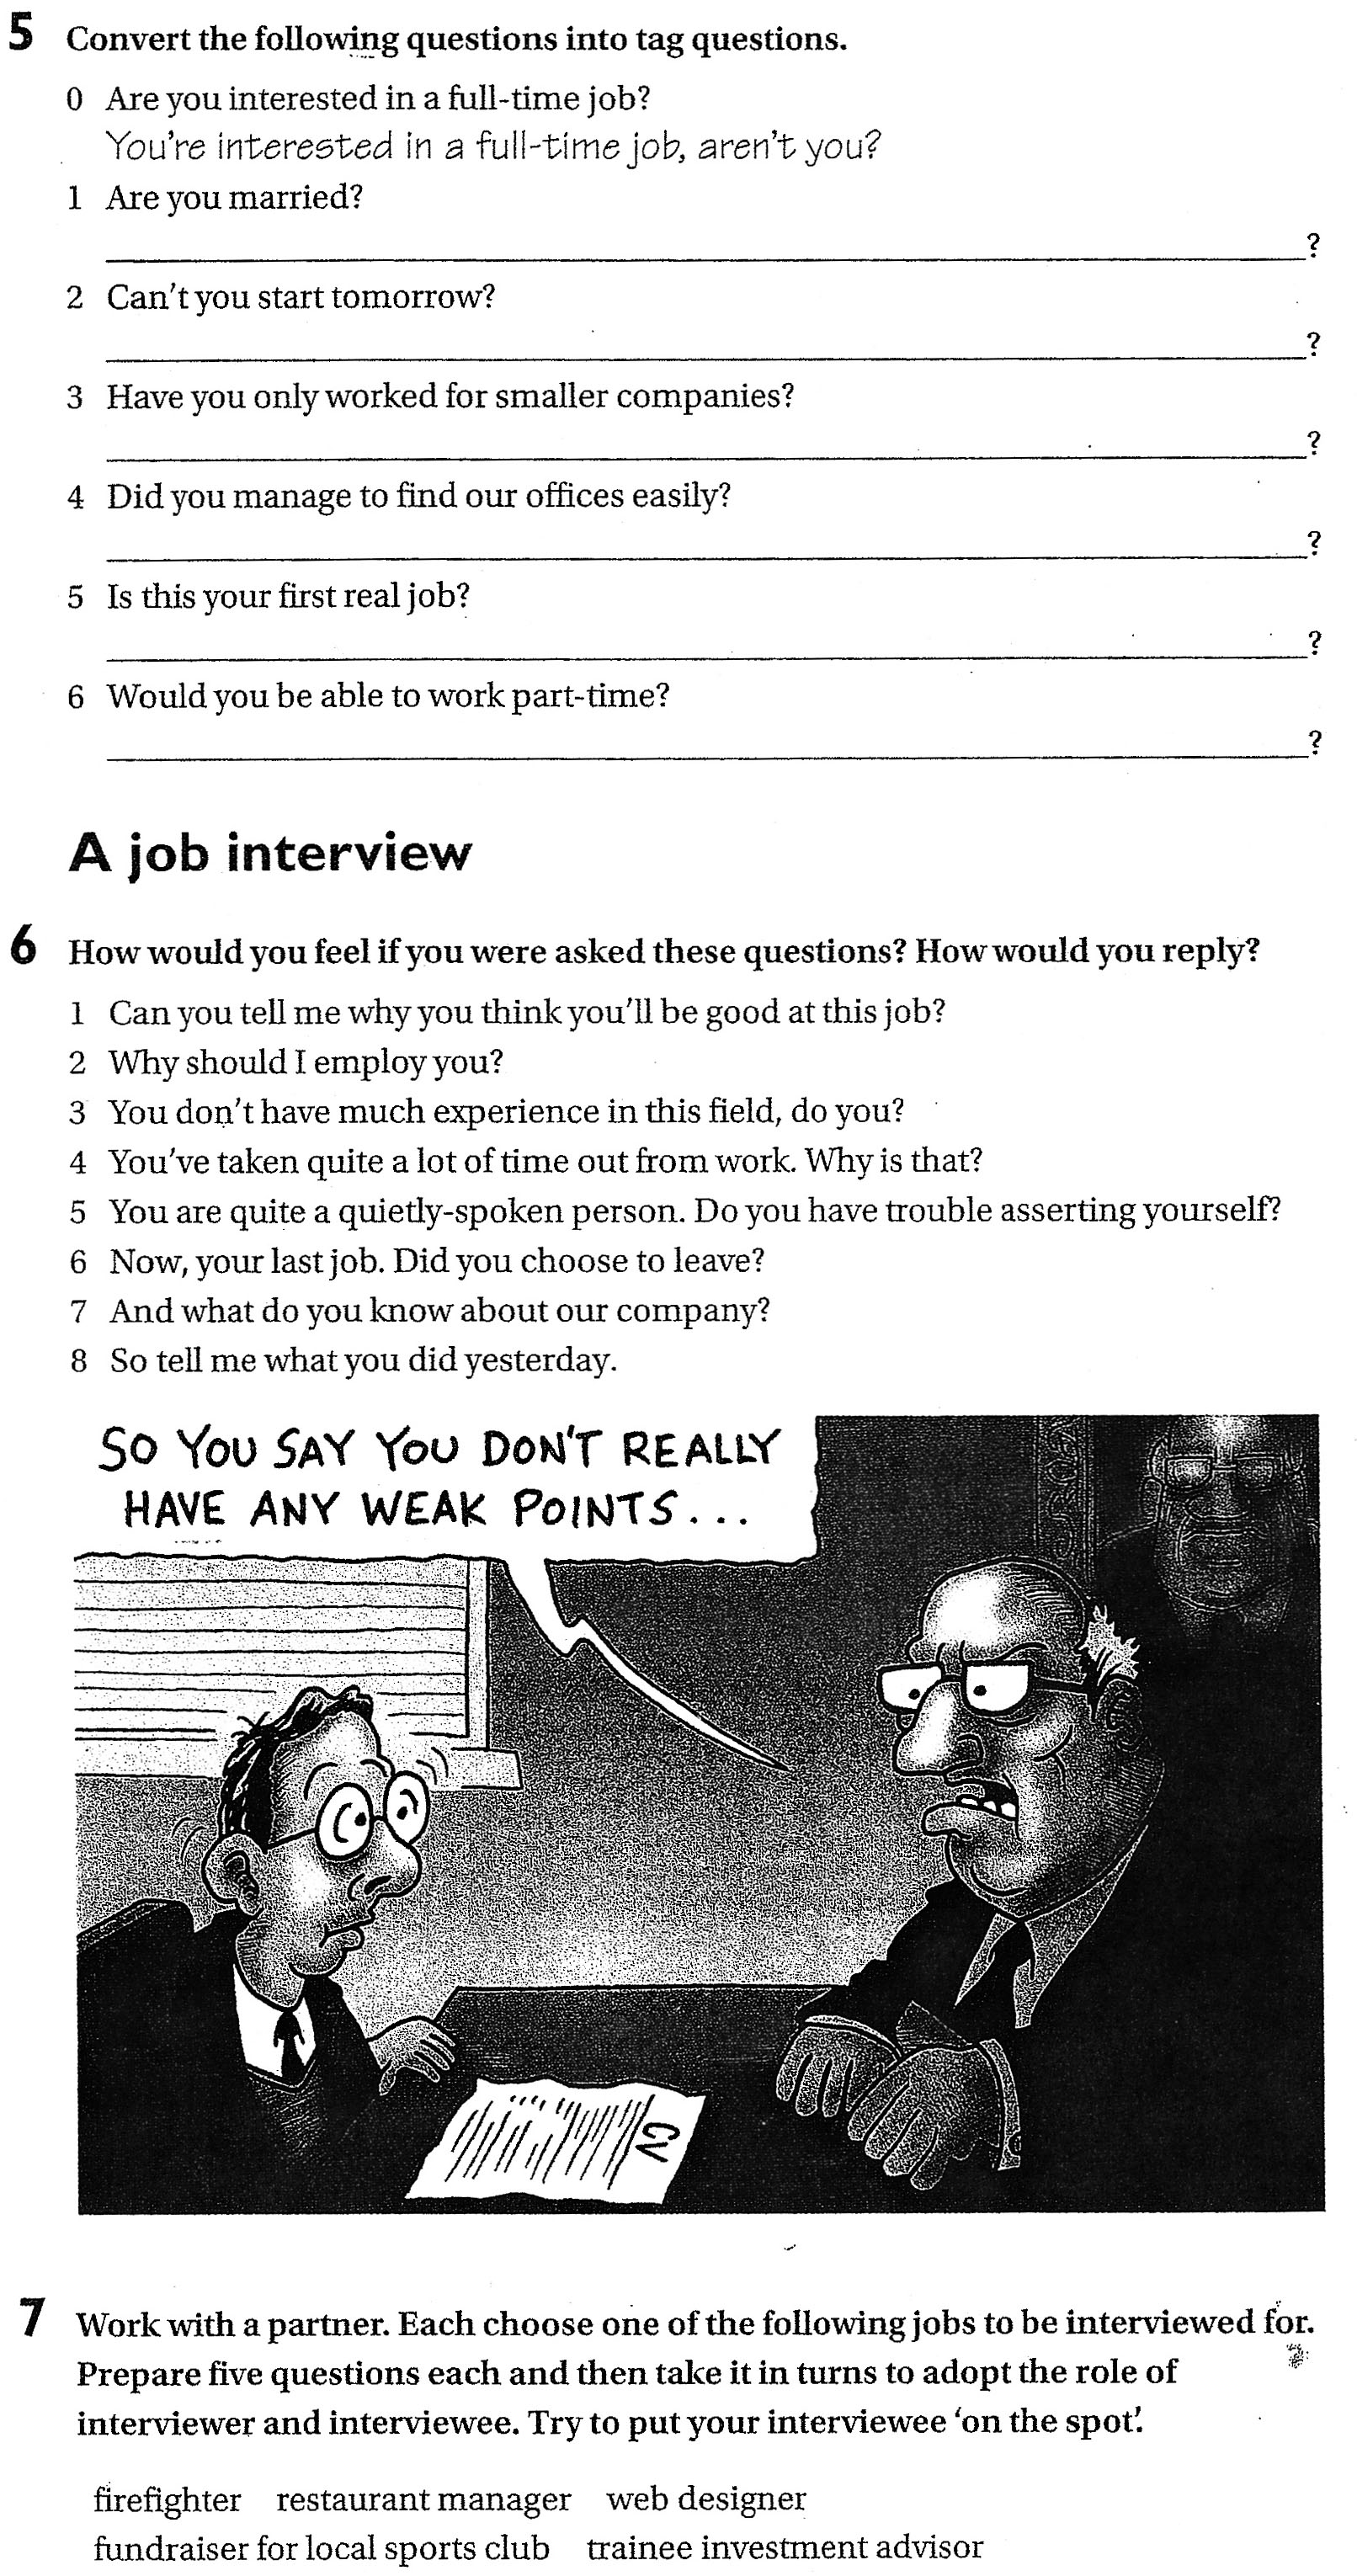
\includegraphics[scale=.85]{handouts/Eng504.jpg}

\chapter{Interviews}
Berkley%\\
%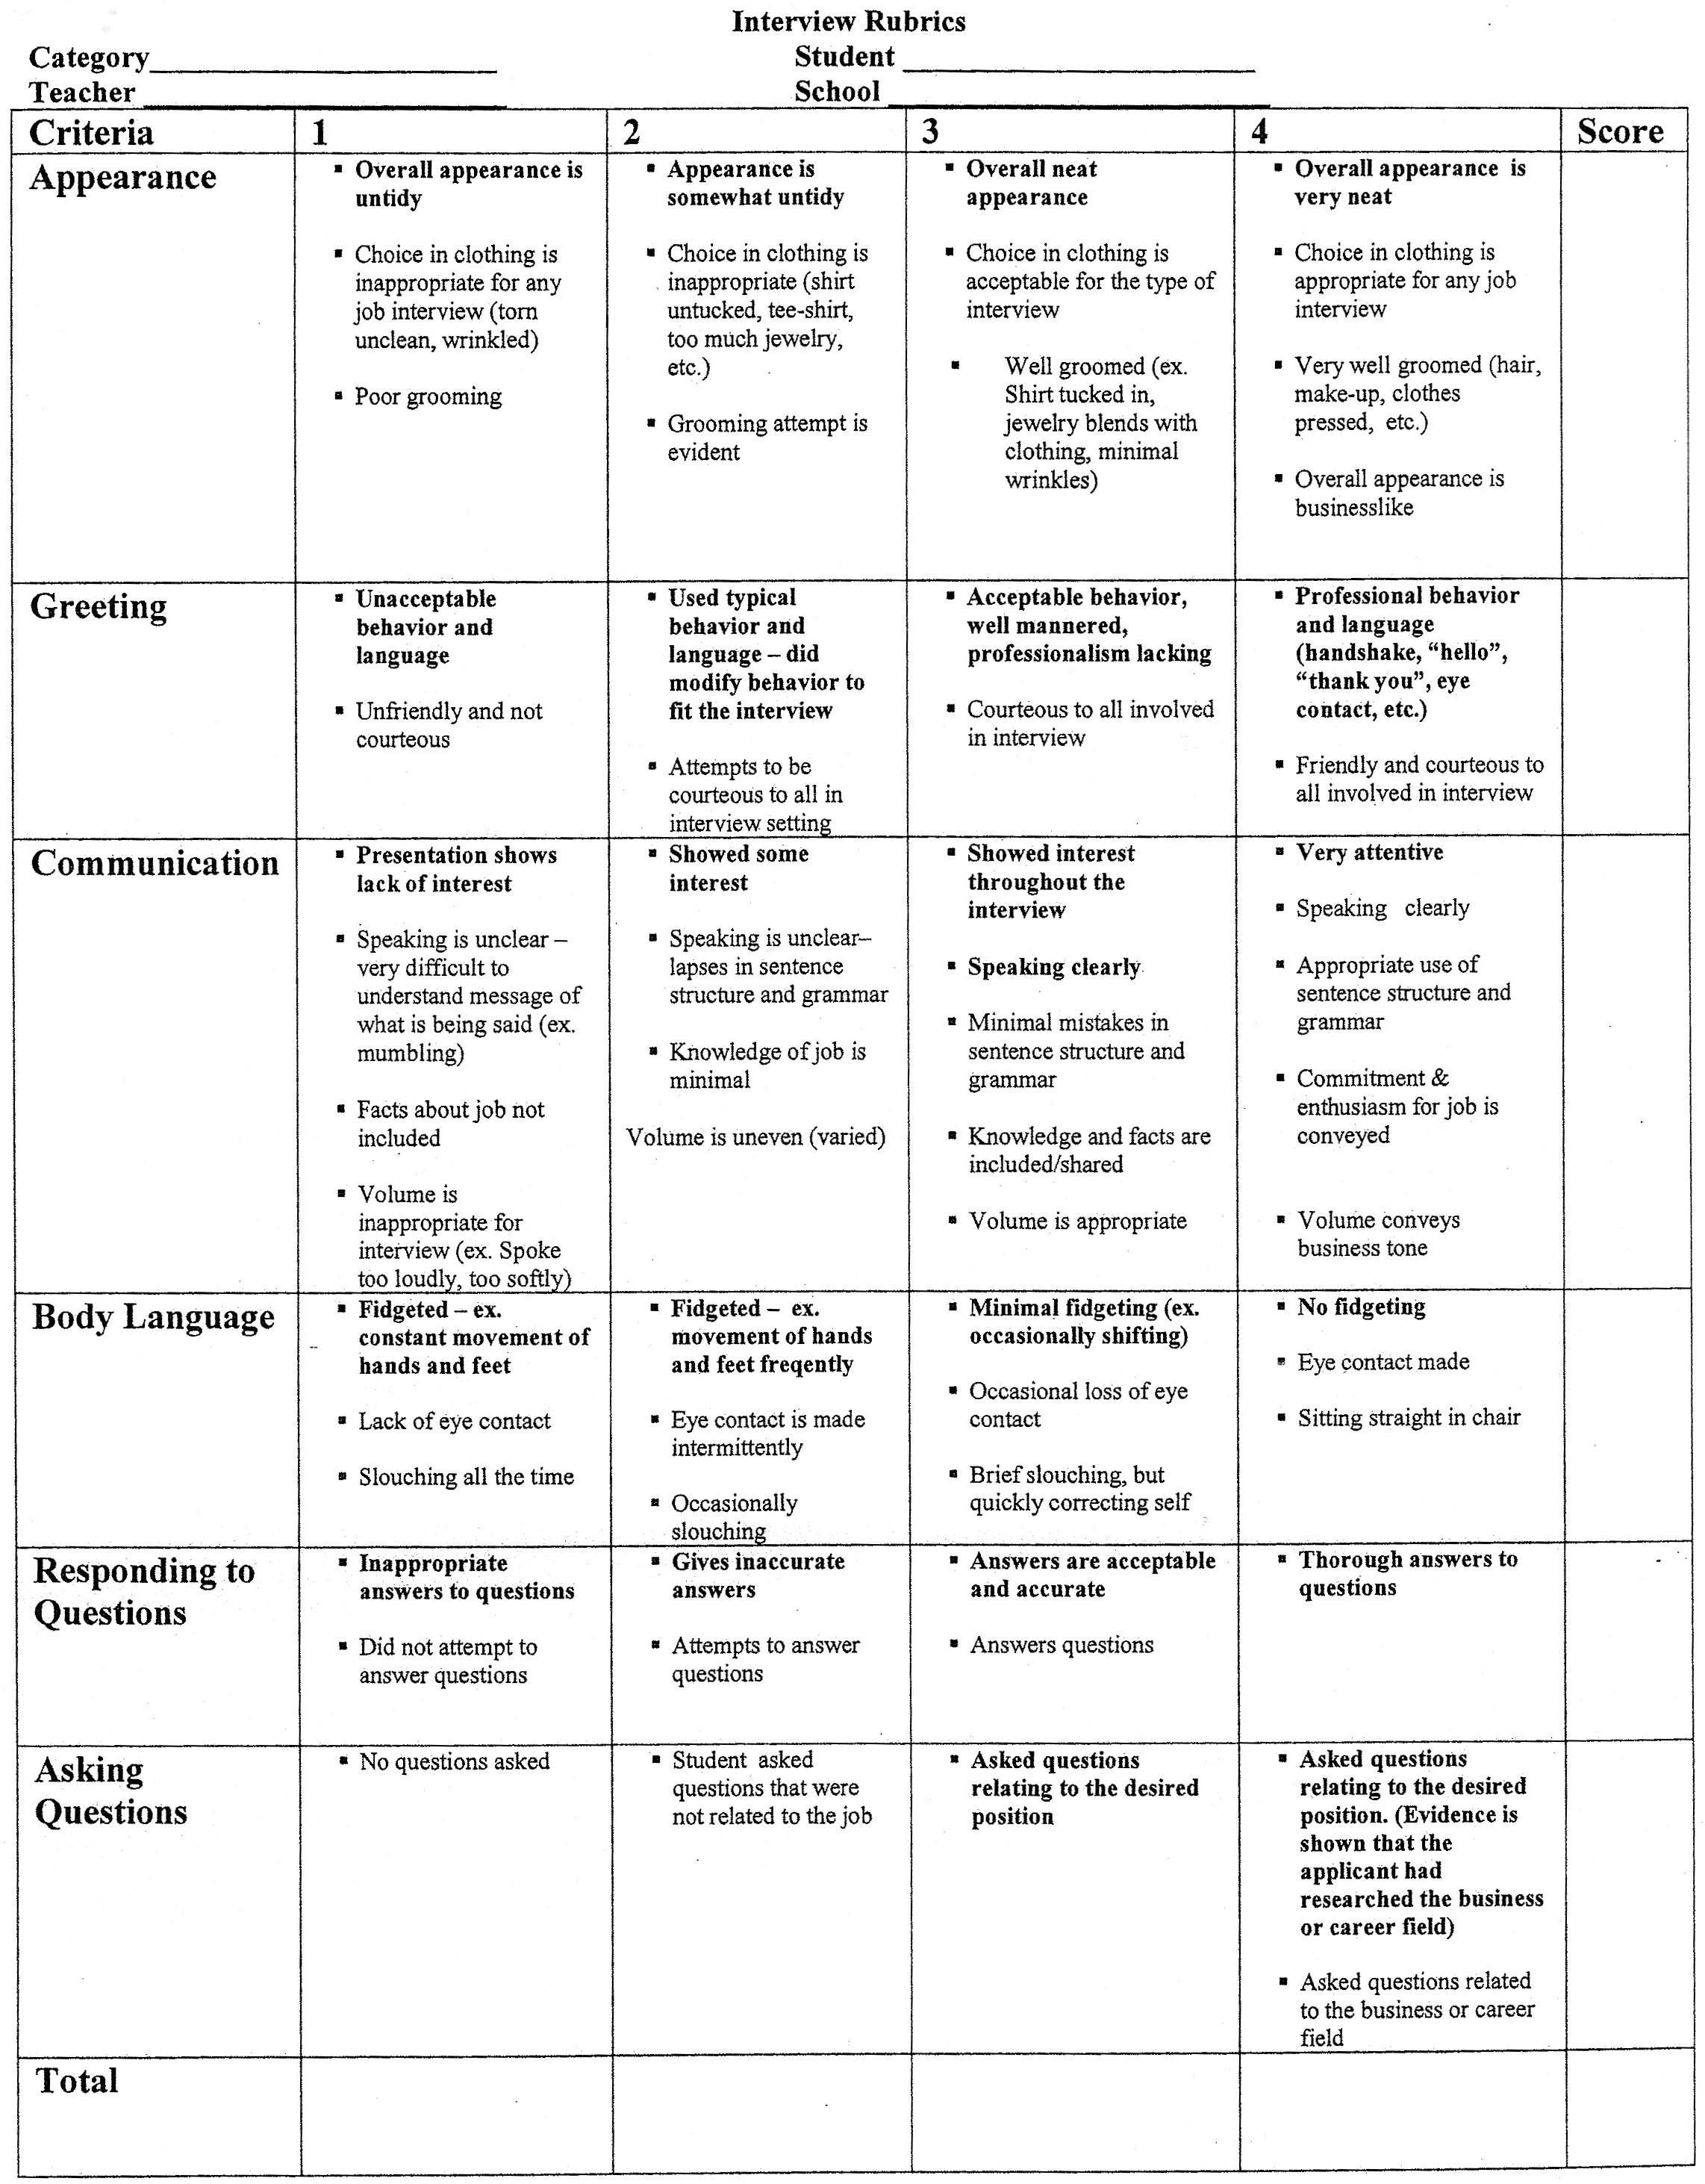
\includegraphics[scale=.85]{handouts/Eng601.jpg}

\chapter{Formal and Informal}
\section{Vocabulary}
\paragraph{Verbs}
\begin{tabular}{l l}
to depart & to go\\
to retain & to keep\\
to cease & to stop\\
to function & to work\\
to masticate & to chew\\
to demonstrate & to show\\
to reside & to live\\
\hline
to appear & to appear\\
to abbreviate & to shorten\\
to terminate & to end\\
to aid & to help\\
to commence & to begin\\
to desire/demand & to want\\
to obtain & to get\\
to liberate & to free\\
to consume & to eat
\end{tabular}

\paragraph{Adverbials}
\begin{tabular}{l l}
subsequently & next/later\\
principally & mainly\\
consequently/therefore & so\\
initially & at first\\
finally & in the end
\end{tabular}

\paragraph{Nouns}
\begin{tabular}{l l}
carnivore & meat-eater\\
putrefaction & decay/rot\\
deficiency & lack\\
vision & sight\\
residence & home\\
respiration & breathing\\
somnambulist & sleep walker\\
comprehension & understanding\\
perspiration & sweat
\end{tabular}

\paragraph{Adjectives}
\begin{tabular}{l l}
incorrect & wrong\\
amible & friendly\\
vacant & empty\\
insane & mad/crazy\\
inexpensive & cheap\\
vivid/vivicios/animated & lively\\
superior/improved & better\\
immature/juvenile/infantile & childish\\
sufficient & enough\\
entire & whole\\
senior & older
\end{tabular}

\section{Phrasal verbs and single-word verbs}
a.)
\begin{enumerate}
\item arrived
\item irritated
\item despaired
\item becoming
\item provoking
\item discussed
\item contacted
\item lodging
\item connected
\item investigated
\item came
\item arranged
\item postponed
\item visited
\item refer
\end{enumerate}
b.)
\begin{enumerate}
\item got
\item put up
\item bring back
\item gone by
\item got
\item worse
\item joined in
\item get on with
\item fell aut
\item turned out
\item making out
\end{enumerate}

\chapter{Products}

Task 9: (Monitor)
\begin{itemize}
\item This device uses multiple LED-lights. These lights compose to a pattern which is interpretable by the human eye. By using this device, complex data may be visualizied for human interaction. This is usefull for humans that want to see a comprehensive representation of a digital correlation.
\item This tool sends out lights that forms a picture. It works together with a computer to display its data on.
\end{itemize}

\paragraph{Audience}
\subparagraph{Used language} \parskp
\begin{tabular}{l l}
expert & theoretical/technical\\
technician & technical/hands-on\\
executive & numbers (project-length, how much it costs, …)\\
non-specialist & basics (with every-day-language)
\end{tabular}

\subparagraph{Audience analysis}
\begin{itemize}
\item background knowledge
\item needs and interests
\item demographics (age, gender)
\end{itemize}

\subparagraph{Audience adaption}
\begin{itemize}
\item add background information
\item omit unneccessary info
\item change the level of info
\item add examples
\item change the level of the examples
\item chaneg the organization of the info
\item strenghten transitions
\item write/give stronger introductions (for the whole and sections)
\item create topic sentences
\item change sentence style and length
\item work on sentence clarity and economy
\item use more or different graphics
\item break up texts into meaningful chunks (shorter paragraphs)
\item add cross-references
\item use headings and lists
\item use special typography
\end{itemize}


\chapter{Presentation}
Object oriented programming/modelling
\begin{itemize}
\item not needed
\begin{itemize}
\item feasabilty
\item information sources
\item graphical aids, expenses
\end{itemize}
\item less important
\begin{itemize}
\item proceedure (of information-gathering)
\end{itemize}
\item important
\begin{itemize}
\item background (class members)
\item proposal
\item benefits
\item results (regarding all: report, presentation, handout)
\item bibliography
\item schedule (draft, presentation, …)
\item qualifications (why subject is chosen)
\item outline
\end{itemize}
\end{itemize}

%\newpage
%\printbibliography
\end{document}